%\documentclass[11pt, a4paper, twoside, openright, draft]{book}
\documentclass[11pt, a4paper, twoside, openright]{book}

%%%%%%%%%%%%%%%%%%%%%%%%%%%%%%%%%%%%%%%%%%%%%%%%%%%%%%%%%%%%%%%%%%%%%%%%%%%%%%%%%%%%%%
%
% File:			packages.tex
%
% Description:	Contains included packages.
%
%%%%%%%%%%%%%%%%%%%%%%%%%%%%%%%%%%%%%%%%%%%%%%%%%%%%%%%%%%%%%%%%%%%%%%%%%%%%%%%%%%%%%%

\usepackage[english]{babel}

\usepackage[T1]{fontenc}
\usepackage{setspace}
\usepackage{fancyhdr}

\usepackage{graphicx}
\usepackage{csquotes}

\usepackage{amsfonts}
\usepackage{amsmath}
\usepackage{amssymb}
\usepackage{amsthm}
\usepackage{bbm}
\usepackage{bm}
\usepackage{gensymb}
\usepackage{mathtools}
\usepackage{relsize}
\usepackage{bbold}
\usepackage{enumitem}
\usepackage{array}
\usepackage{multirow}

\usepackage{layout}

\usepackage{todonotes}

%\usepackage{mathptmx}
\usepackage{newtxtext,newtxmath}


\usepackage[activate={true,nocompatibility},final,tracking=true,kerning=true,spacing=true,factor=1100,stretch=10,shrink=10]{microtype}
% activate={true,nocompatibility} - activate protrusion and expansion
% final - enable microtype; use "draft" to disable
% tracking=true, kerning=true, spacing=true - activate these techniques
% factor=1100 - add 10% to the protrusion amount (default is 1000)
% stretch=10, shrink=10 - reduce stretchability/shrinkability (default is 20/20)
\setlength{\parskip}{0pt}

\usepackage[%
backend=biber,%
style=phys,%
articletitle=true,biblabel=brackets,%
chaptertitle=false,pageranges=false%
]
{biblatex}
\addbibresource{master.bib}
\AtBeginDocument{\renewcommand{\bibname}{References}} 


%\usepackage[Lenny]{fncychap}

%\usepackage{bm}

%\usepackage{mathspec}


%\usepackage{wrapfig}
\usepackage[normal, bf, footnotesize]{caption}
\usepackage[breaklinks]{hyperref}
\hypersetup{colorlinks = true, linkcolor=black, citecolor=black, urlcolor=black}
\usepackage{pdfpages}
%\usepackage[outer=2.0cm, inner=2.7cm, top=4.0cm, bottom=2.4cm, headsep=1.5cm]{geometry}
\usepackage{ifthen}
\usepackage{blindtext}
%\usepackage[activate{true,nocompatability}]{microtype}

\newcolumntype{L}[1]{>{\raggedright\let\newline\\\arraybackslash\hspace{0pt}}m{#1}}
\newcolumntype{C}[1]{>{\centering\let\newline\\\arraybackslash\hspace{0pt}}m{#1}}
%%%%%%%%%%%%%%%%%%%%%%%%%%%%%%%%%%%%%%%%%%%%%%%%%%%%%%%%%%%%%%%%%%%%%%%%%%%%%%%%%%%%%%
%
% File:			headerGeneral.tex
%
% Description:	Contains general layout settings
%
%%%%%%%%%%%%%%%%%%%%%%%%%%%%%%%%%%%%%%%%%%%%%%%%%%%%%%%%%%%%%%%%%%%%%%%%%%%%%%%%%%%%%%

%\onehalfspacing

\setstretch{1.3}

%\usetikzlibrary{calc,matrix,backgrounds,positioning}
%\pgfdeclarelayer{myback}
%\pgfsetlayers{myback,background,main}

\graphicspath{{../figures/}}

%%%%%%%%%%%%%%%%%%%%%%%%%%%%%%%%%%%%%%%%%%%%%%%%%%%%%%%%%%%%%%%%%%%%%%%%%%%%%%%%%%%%%%
%
% File:			headerPhysics.tex
%
% Description:	Contains (mostly) useful commands for writing mathematics and physics.
%
%%%%%%%%%%%%%%%%%%%%%%%%%%%%%%%%%%%%%%%%%%%%%%%%%%%%%%%%%%%%%%%%%%%%%%%%%%%%%%%%%%%%%%

\makeatletter % Need for anything that contains an @ command 
\renewcommand{\labelenumi}{(\alph{enumi})} % Use letters for enumerate
% \DeclareMathOperator{\Sample}{Sample}
\let\vaccent=\v % rename builtin command \v{} to \vaccent{}


\newcommand{\expv}[1]{\langle #1 \rangle}
\newcommand{\vareps}{\varepsilon}
\newcommand{\tbf}[1]{\textbf{#1}}
\newcommand{\bv}[1]{\bm{#1}} % for vectors

\renewcommand{\Re}{\mathfrak{Re}}
\renewcommand{\Im}{\mathfrak{Im}}

\newcommand{\prm}{\ensuremath{^{\prime}}}

\newcommand{\op}[1]{\ensuremath{\hat{#1}}}

\renewcommand{\i}{\ensuremath{\text{i}}} % imaginary

\newcommand{\donehalf}{\dfrac{1}{2}}
\newcommand{\onehalf}{\frac{1}{2}}

\newcommand{\infint}[1]{\int\limits_{-\infty}^{\infty}{#1}}
\newcommand{\trace}{\text{Tr}}

\newcommand{\meas}[2]{\text{d}^\ensuremath{{#1}\text{#2}}\,}
%\newcommand{\m}[2]{\ensuremath{\text{#1 #2}}}

\newcommand{\gv}[1]{\ensuremath{\mbox{\boldmath$ #1 $}}} 
% for vectors of Greek letters

\newcommand{\uv}[1]{\ensuremath{\mathbf{\hat{#1}}}} % for unit vector
\newcommand{\abs}[1]{\left| #1 \right|} % for absolute value
\newcommand{\Avg}[1]{\langle #1 \right\rangle} % for average
\newcommand{\avg}[1]{\langle #1 \rangle} % for average
\let\underdot=\d % rename builtin command \d{} to \underdot{}
\renewcommand{\d}[2]{\frac{d #1}{d #2}} % for derivatives
\newcommand{\dd}[2]{\frac{d^2 #1}{d #2^2}} % for double derivatives
\newcommand{\pd}[2]{\frac{\partial #1}{\partial #2}} 
% for partial derivatives
\newcommand{\pdd}[2]{\frac{\partial^2 #1}{\partial #2^2}} 
% for double partial derivatives

\newcommand{\pdc}[3]{\left( \frac{\partial #1}{\partial #2}
 \right)_{#3}} % for thermodynamic partial derivatives
\newcommand{\dfr}[2]{\dfrac{#1}{#2}}

\newcommand{\ketbra}[1]{\left| #1\rangle \langle #1\right|}
\newcommand{\matrixel}[3]{\left< #1 \vphantom{#2#3} \right|
 #2 \left| #3 \vphantom{#1#2} \right>} % for Dirac matrix elements
\newcommand{\grad}[1]{\gv{\nabla} #1} % for gradient
\let\divsymb=\div % rename builtin command \div to \divsymb
\renewcommand{\div}[1]{\gv{\nabla} \cdot #1} % for divergence
\newcommand{\curl}[1]{\gv{\nabla} \times #1} % for curl
\let\accent=\= % rename builtin command \= to \baraccent
\renewcommand{\=}[1]{\stackrel{#1}{=}} % for putting numbers above =
% \newtheorem{prop}{Proposition}
% \newtheorem{thm}{Theorem}[section]
% \newtheorem{lem}[thm]{Lemma}
% \theoremstyle{definition}
% \newtheorem{dfn}{Definition}
% \theoremstyle{remark}
% \newtheorem*{rmk}{Remark}

% Bra-Ket notation
\newcommand{\Ket}[1]{\left| #1 \right\rangle} % for Dirac kets
\newcommand{\Bra}[1]{\left\langle #1 \right|} % for Dirac bras 
\newcommand{\ket}[1]{| #1 \rangle} % for Dirac kets
\newcommand{\bra}[1]{\langle #1 |} % for Dirac bras 
\newcommand{\Braket}[2]{\left\langle #1 \vphantom{#2} \right|
 \left. #2 \vphantom{#1} \rangle>} % for Dirac brackets

% (Anti-) Commutators
\newcommand{\comm}[2]{\ensuremath{\left[#1,~#2\right]}}
\newcommand{\anticomm}[2]{\ensuremath{\left\{#1,~#2\right\}}}

\newcommand{\mc}[1]{\ensuremath{\mathcal{#1}}}
\newcommand{\mb}[1]{\ensurement{\mathbb{#1}}}

% (Dirac)-Adjoint
\renewcommand{\dag}{\ensuremath{^{\dagger}}}
\newcommand{\dadj}[1]{\ensuremath{\overline{#1}}}
\newcommand{\ansatz}[1]{\ensuremath{\overline{#1}}}
\newcommand{\cc}[1]{\ensuremath{\overline{#1}}}

% Identity operator
%\newcommand{\id}{\ensuremath{\mathds{1}}}
\newcommand{\id}{\ensuremath{\mathbbm{1}}}
\newcommand{\ZZ}{\ensuremath{\mathbb{Z}_{2}}}

% Inverse operation
\newcommand{\inv}{\ensuremath{^{-1}}}

% Tilde
\newcommand{\til}[1]{\ensuremath{\widetilde{#1}}}

% Lithium Iridates
\newcommand{\sodiumIridate}{Na$_2$IrO$_3$}
\newcommand{\alphaLithiumIridate}{$\alpha$-Li$_2$IrO$_3$}
\newcommand{\betaLithiumIridate}{$\beta$-Li$_2$IrO$_3$}
\newcommand{\gammaLithiumIridate}{$\gamma$-Li$_2$IrO$_3$}
\newcommand{\ruthiniumTriChloride}{RuCl$_3$}

% Effective Hamiltonian
\newcommand{\heff}{\ensuremath{\til{H}_\text{eff}}}

% Weyl Hamiltonian
\newcommand{\hweyl}{\ensuremath{H_\text{Weyl}}}

% Often used vectors
\newcommand{\bR}{\bv{R}}
\newcommand{\br}{\bv{r}}
\newcommand{\bz}{\bv{0}}
\newcommand{\bx}{\bv{x}}
\newcommand{\by}{\bv{y}}
\newcommand{\ba}{\bv{a}}
\newcommand{\bq}{\bv{q}}
\newcommand{\bk}{\bv{k}}
\newcommand{\bp}{\bv{p}}
\newcommand{\bP}{\bv{P}}
\newcommand{\bb}{\bv{b}}
\newcommand{\bc}{\bv{c}}
\newcommand{\bsigma}{\bm{\sigma}}
\newcommand{\btau}{\bm{\tau}}
\newcommand{\bS}{\bv{S}}

% Signum
\DeclareMathOperator{\signum}{sgn}

% Latin abbreviations
\newcommand{\ie}{{\it i.e.}}
\newcommand{\eg}{{\it e.g.}}


%\raggedbottom

\fancypagestyle{plain}{%
	\fancyhf{}
	\fancyfoot{}
	\renewcommand{\headrulewidth}{0pt}
	\renewcommand{\footrulewidth}{0pt}
}

\usepackage{afterpage}
\setlength{\marginparwidth}{2.5cm}

%%%%%%%%%%%%%%%%%%%%%%%%%%%%%%%%%%%%%%%%%%%%%%%%%%%%%%%%%%%%%%%%%%%%%%%%%%%%%%%%%%%%%%%%
%
%
\begin{document}
%
%
%%%%%%%%%%%%%%%%%%%%%%%%%%%%%%%%%%%%%%%%%%%%%%%%%%%%%%%%%%%%%%%%%
% FRONT MATTER
%%%%%%%%%%%%%%%%%%%%%%%%%%%%%%%%%%%%%%%%%%%%%%%%%%%%%%%%%%%%%%%%%
%
%
\pagestyle{empty}
\pagenumbering{gobble}
\hypersetup{pageanchor=false}

%%%%%%%%%%%%%%%%%%%%
%  FOR WEB ONLY  %
%%%%%%%%%%%%%%%%%%%%

\includepdf[fitpaper=true, pages=-]{./a4_cover.pdf}
%%%%%%%%%%%%%%%%%%%%

\begin{titlepage}

	\vspace*{\fill}
	\begin{center}
		
		{\Huge\textbf{Three-Dimensional\\
				\vspace{0.5cm}
				Kitaev Spin Liquids}}\\
		\vspace{1.5cm}
	
		\doublespacing
		\textbf{Inaugural-Dissertation}\\
		zur\\
		Erlangung des Doktorgrades\\
		der Mathematisch-Naturwissenschaftlichen Fakult\"{a}t\\
		der Universit\"{a}t zu K\"{o}ln\\
		vorgelegt von\\
		
		\vspace{0.5cm}
		{\Large\textbf{Kevin Michael O'Brien}}\\
		\vspace{0.5cm}

		\normalsize
		aus Cleveland, Ohio\\
%		The United States of America\\

		\vspace{1.cm}		
		\begin{figure}[h!]
			\centering
			
\includegraphics[height=5cm]{./titlePage/SiegelMatNat.pdf}
		\end{figure}
		\vspace{1.0cm}
				
		K\"{o}ln 2019
	\end{center}
	\vspace*{\fill}

\end{titlepage}

\onehalfspacing


\noindent
\begin{tabular}{ll}
	Berichtserstatter: \hspace{2cm} & Prof. Dr. Simon Trebst \\
		   & Prof. Dr. Achim Rosch\\
		   & \\
		   & \\
	Tag der m\"{u}ndlichen Pr\"{u}fung: & xx.xx.2019
\end{tabular}

\singlespacing
%%%%%%%%%%%%%%%%%%%%%%%%%%%%%%%%%%%%%%%%%%%%%%%%%%%%%%%%%%%%%%%%%%%%%%%%%%%%%%%%%%%%%%%%
\chapter*{Abstract}
%%%%%%%%%%%%%%%%%%%%%%%%%%%%%%%%%%%%%%%%%%%%%%%%%%%%%%%%%%%%%%%%%%%%%%%%%%%%%%%%%%%%%%%%
%
%
The formation of quantum spin liquids in frustrated magnets represents an exciting possibility due to the rather exotic features they harbor, including fractionalized excitations and emergent gauge fields.
Unfortunately, they are notoriously difficult to study as there are often no good analytical methods available and quantum Monte Carlo simulations are hindered by the negative sign problem.
The Kitaev honeycomb model is a notable exception of a frustrated quantum model which is exactly solvable and which hosts a number of distinct quantum spin liquid ground states.
As such, it allows for a rare opportunity to study the physics of spin liquids with full analytical control.

In this thesis, we study the fractionalization of spin-1/2 moments into Majorana fermions and an emergent \ZZ~gauge field in a generalization of the Kitaev honeycomb model to a number of three-dimensional lattices.
While the excitations of the gauge field are always gapped, the fermionic quasiparticles may exhibit a gapless dispersion, forming fully two-dimensional Fermi surfaces, symmetry protected nodal lines, or topological Weyl nodes.
We show that one can deduce rather general constraints on the possible gapless excitations by making use of an object called the projective symmetry group.
In doing so we provide a scheme for classifying the various gapless Kitaev spin liquids.
A thorough analysis is carried out for a number of these spin liquids, primarily investigating the stability of the gapless modes and the novel features resulting from their sometimes non-trivial topology, as well as their effects on certain equal-time correlation functions.
%%%%%%%%%%%%%%%%%%%%%%%%%%%%%%%%%%%%%%%%%%%%%%%%%%%%%%%%%%%%%%%%%%%%%%%%%%%%%%%%%%%%%%%%
\chapter*{Kurzzusammenfassung}
%%%%%%%%%%%%%%%%%%%%%%%%%%%%%%%%%%%%%%%%%%%%%%%%%%%%%%%%%%%%%%%%%%%%%%%%%%%%%%%%%%%%%%%%
%
%
Die Bildung von Quanten-Spinfl\"ussigkeiten in frustrierten Magneten stellt eine aufregende M\"oglichkeit dar, da sie ziemlich exotische Eigenschaften aufweisen, wie z. B. fraktionalisierte Anregungen und auftauchende Eichfelder.
Leider sind sie bekannterma\ss en schwer zu untersuchen, da oft keine guten Analysemethoden verf\"ugbar sind und Quanten-Monte-Carlo-Simulationen durch das Problem der negativen Vorzeichen nicht verwendbar werden.
Das Kitaev-Modell ist eine bemerkenswerte Ausnahme eines frustrierten Quantenmodells, das genau l\"osbar ist und eine Reihe unterschiedlicher Quanten-Spinfl\"ussigkeit-Grundzust\"ande enth\"alt.
Daher bietet es die seltene Gelegenheit, die Physik von Spinfl\"ussigkeiten mit voller analytischer Kontrolle zu untersuchen.

In dieser Arbeit untersuchen wir die Fraktionalisierung von Spin-1/2-Momenten in Majorana-Fermionen und ein aufkommendes \ZZ-Eichfeld in einer Ver\-all\-ge\-mei\-ne\-rung des Kitaev-Modells auf eine Anzahl dreidimensionaler Gitter.
W\"ahrend die Anregungen des Eichfeldes immer gegapped sind, k\"onnen die fermionischen Quasiteilchen eine gapless Dispersion aufweisen, die vollst\"andig zweidimensionale Fermi-Fl\"achen, wegen Symmetrie gesch\"utzte Knotenlinien oder topologische Weyl-Knoten bildet.
Wir zeigen, dass man eher allgemeine Einschr\"ankungen f\"ur die m\"oglichen gapless Anregungen ableiten kann, indem man ein Objekt verwendet, das als \textit{Projective Symmetry Group} bezeichnet wird.
Damit stellen wir ein Schema zur Klassifizierung der verschiedenen gapless Kitaev-Spin-Fl\"ussigkeiten bereit.
F\"ur eine Anzahl dieser Spin-Fl\"ussigkeiten wird eine gr\"undliche Analyse durchgef\"uhrt, wobei vor allem die Stabilit\"at der gapless Moden und die neuen Merkmale untersucht werden, die sich aus ihrer manchmal nicht-trivialen Topologie ergeben, sowie deren Auswirkungen auf bestimmte Korrelationsfunktionen.

\newpage
\mbox{}
\newpage
~\\[5cm]
\begin{center}
	{\Huge To my parents.}
\end{center}

\onehalfspacing
\tableofcontents


%%%%%%%%%%%%%%%%%%%%%%%%%%%%%%%%%%%%%%%%%%%%%%%%%%%%%%%%%%%%%%%%%
% MAIN MATTER
%%%%%%%%%%%%%%%%%%%%%%%%%%%%%%%%%%%%%%%%%%%%%%%%%%%%%%%%%%%%%%%%%
%
%
\normalsize
\singlespacing
\newpage
\thispagestyle{empty}
\mbox{}
\newpage
\setcounter{page}{1}
\hypersetup{pageanchor=true}
\pagestyle{fancy}
\fancyhead{}
\setlength{\headheight}{13.6pt}
\fancyhead[RE]{\nouppercase\leftmark}
\fancyhead[LE]{\textbf{\thepage}}
\fancyhead[LO]{\nouppercase\rightmark}
\fancyhead[RO]{\textbf{\thepage}}
\cfoot{}
\pagenumbering{arabic}


%%%%%%%%%%%%%%%%%%%%%%%%%%%%%%%%%%%%%%%%%%%%%%%%%%%%%%%%%%%%%%%%%%%%%%%%%%%%%%%%%%%%%%%%
\chapter{Introduction}
\label{chapter:Introduction}
%%%%%%%%%%%%%%%%%%%%%%%%%%%%%%%%%%%%%%%%%%%%%%%%%%%%%%%%%%%%%%%%%%%%%%%%%%%%%%%%%%%%%%%%
%
%
In the study of quantum many-body systems, perhaps the most profound and influential ideas have been those of Landau's theory of phase transitions~\cite{LandauNature1936,LandauZETF1937,GinzburgZETF1950} coupled with Wilson's notions of universality~\cite{WilsonPRB1971I,WilsonPRB1971II,WilsonPRL1972,WilsonRMP1975} and Landau's Fermi liquid theory~\cite{LandauZETF1956,LandauZETF1957,LandauZETF1958}.
The former provided an understanding of different phases of matter in terms of their differing symmetries and characterized the phase transition in terms of a quantity called the \textit{order parameter} which signals the spontaneous breaking of a symmetry in the system.
A broken symmetry phase is said to be \textit{ordered} as the microscopic constituents of the system are correlated with one another over large distances.
Wilson's ideas showed that phase transitions from very different contexts exhibit certain universal characteristics and may be grouped into so-called \textit{universality classes} defined by their critical behavior.
Landau's Fermi liquid theory allowed for the description of interacting electrons in a metal in terms of nearly free electron-like \textit{quasiparticles} -- collective excitations which have the same charge as the electron, but with an effective mass which differs from that of the electron.

These ideas proved so successful at comprehensively classifying matter for so many years, it signaled a true paradigm shift in condensed matter physics when Tsui, St\"ormer and Gossard discovered the fractional quantum Hall effect~\cite{TsuiPRL1982} in 1982, revealing a phase of matter which evaded understanding in these terms.
In a fractional quantum Hall liquid, the transverse -- or Hall -- conductance of two-dimensional electrons in a strong magnetic field shows precisely and robustly quantized plateaus at fractional values of $e^2/h$ as a function of magnetic field strength, where $e$ is the fundamental charge and $h$ is Planck's constant.
Changing the strength of the magnetic field causes the system to undergo a phase transition from one plateau to another.
However, different fractional quantum Hall states all have the same symmetry and, thus, cannot be described in terms of symmetry breaking.
Furthermore, the excitations in the system cannot be described by the Fermi liquid theory.
This ushered in the realization that there exist phases of matter beyond the reach of Landau's theories and that the concept of order must be expanded~\cite{WenJMPB1990,WenAiP1995,WenPRB2002,WenPLA2002}.

Such systems exhibiting \textit{quantum} or \textit{topological orders} can feature novel properties such as gapless edge modes~\cite{HalperinPRB1982,HatsugaiPRL1993,SchulzBaldesJPA2000,KellendonkRMaP2002} or fractionalized excitations~\cite{LaughlinPRL1983,LaughlinIJM1991,dePicciottoNature1997}, \ie, collective excitations whose quantum numbers are fractions of those of the original constituents of the system.
An example of fractionalized excitations are the quasihole excitations in the $\nu = 1/3$ fractional quantum Hall system which carry a charge equal to one-third that of the electron.
These fractionalized excitations can obey statistics other than those of bosons or fermions.
Such \textit{anyons} may acquire an arbitrary phase upon being exchanged -- so-called \textit{Abelian anyons}~\cite{LeinaasNCSIF1977,WilczekPRL1982,GoldinJMP1981,WuPRL1984} -- or, in some cases, exchange of particles corresponds to a non-commuting operation, giving rise to so-called \textit{non-Abelian anyons}~\cite{MoorePLB1988,Witten1989}.
One of the more tantalizing prospects offered by these phases of matter is the realization of a fault-tolerant, topological quantum computer, wherein information is stored non-locally in states with multiple non-Abelian quasiparticles~\cite{MoessnerPRL2001,LevinRMP2005,LevinPRB2005,NayakRMP2008}.

Another phase categorized by such unconventional "order" which is more germane to this thesis is the \textit{quantum spin liquid}.
In a quantum spin liquid phase, interacting spins evade magnetic order down to zero temperature as a result of strong quantum fluctuations whilst maintaining a high degree of correlation due to their interactions.
The lack of magnetic order for any temperature means that a quantum spin liquid falls outside the purview of Landau's traditional order, however, it does not provide for a positive identification of what a spin liquid is.
A more modern point of view~\cite{SavaryRPP2016} posits that the lack of order is not the essential ingredient of a quantum spin liquid, rather it is the anomalously high degree of entanglement which accompanies it.
This massive many-body entanglement allows these states to support the kind of non-local, fractionalized excitations mentioned above.

Historically, the idea of the quantum spin liquid was introduced in the form of the resonating valence bond (RVB) state by Anderson as a possible ground state for a spin-1/2 Heisenberg antiferromagnet~\cite{AndersonMRB1973}.
An RVB state comprises a quantum superposition of states wherein every pair of spins forms a singlet.
The notion was popularized again years later in the context of high-temperature superconductivity~\cite{AndersonScience1987,BaskaranSSC1987}.
This work introduced a fermionic description of the spin liquid state later used by Wen~\cite{WenPRB2002,WenPLA2002} to characterize the quantum order of spin liquids using a mathematical object called the \textit{projective symmetry group}.

On the experimental side, there have been several candidate spin liquid materials over the years.
Perhaps the best studied examples are the triangular-lattice compounds $\kappa$-(ET)$_2$Cu$_2$(CN)$_3$~\cite{ShimizuPRL2003} and Pd$({\rm dmit})_2$(EtMe$_3$Sb)~\cite{ItouPRB2008}, both of which show no long-range magnetic order down to $\sim 30$ mK -- four orders of magnitude smaller than the exchange coupling strengths.
Additionally, the kagome compound ZnCu$_3({\rm OH})_6$Cl$_2$~\cite{HeltonPRL2007} and the three-dimensional hyperkagome material\linebreak Na$_4$Ir$_3$O$_8$~\cite{OkamotoPRL2007} are considered to be candidates for quantum spin liquids with gapless excitations~\cite{OlariuPRL2008,ImaiPRL2008,LawlerPRL2008,ZhouPRL2008}.

Although much progress has been made over the years concerning quantum spin liquids~\cite{SavaryRPP2016}, the competing interactions and frustration necessary to give rise to such disordered quantum liquids means that models which are both exactly solvable and realistic are hard to come by.
One model which fits both of these criteria is Kitaev's now famous honeycomb model~\cite{KitaevAoP2006} -- the star of this thesis.
The model Hamiltonian looks simple, describing a system of spin-1/2 moments on a honeycomb lattice with nearest-neighbor Ising exchange.
However, the component of spin which is coupled depends on the direction of the bond connecting the two spins -- an example of a quantum compass model~\cite{KugelSPU1982} characterized by an exchange interaction only between certain components of the spin and for which different components are coupled for different bonds~\cite{NussinovRMP2015}.
The inability to satisfy the incompatible local Ising constraints results in a system of frustrated spins which exhibit no long-range order down to zero temperature.
The quantum spin liquid ground state hosts fractionalized excitations corresponding to fluxes of an emergent \ZZ~gauge field and fermions which may be either gapped or gapless depending on the values of the exchange couplings.
The gapped phase has been shown to host Abelian anyon excitations and, under application of a magnetic field, the fermions in the gapless phase are gapped out and the resulting excitations are non-Abelian anyons.

However, just because a model is simple to write down does not make it useful.
Typically, interacting models do not lend themselves to exact solution and the frustrated nature of the interactions greatly complicates numerical techniques such as quantum Monte Carlo.
One of the things that makes the Kitaev honeycomb model so important is that it possesses an exact solution, allowing for full analytic control in exploring the complex physics of its ground state phase diagram.
The original solution to the model involves rewriting the spin-1/2 Hamiltonian in terms of Majorana fermions hopping in a static \ZZ~gauge field -- ultimately being reduced to a theory of free fermions.

While the simplicity and exact solvability of Kitaev's honeycomb model make it very attractive to theorists, it was the work of Jackeli and Khaliullin~\cite{JackeliPRL2009} which made it relevant to experimentalists by revealing the applicability of the model to certain spin-orbit entangled Mott insulators with heavy transition metal ions.
This work sparked an intense effort to find materials exhibiting such frustrated, bond-dependent interactions.
In the search for Kitaev materials, prominent examples include the honeycomb iridates Na$_2$IrO$_3$~\cite{SinghPRB2010}, $\alpha$-Li$_2$IrO$_3$~\cite{KobayashiJMC2003,SinghPRL2012} and the ruthenate $\alpha$-RuCl$_3$.
Additionally, experimentalists have found iridate compounds with dominant Kitaev-type interactions realizing fully three-dimensional lattices as well~\cite{TakayamaPRL2015,LeePRB2015,KimEPL2015,LeePRB2016,KatukuriSP2016,ModicNatComm2014,BiffinPRL2014,KimchiPRB2014}.
As will be discussed in more detail later in this thesis, all of these materials exhibit long-range magnetic order at finite temperatures and a more realistic description should include additional exchange interactions.

Although such considerations are necessary to realistically describe these materials, the pure Kitaev model still has much to offer on its own.
This is particularly true when considering its extension to three-dimensional, tricoordinated lattices where it maintains its exact solvability.
It is precisely this rich and diverse Kitaev spin liquid physics which is the focus of this thesis.
The work reported here is mainly concerned with the gapless Kitaev spin liquids which appear in a number of tricoordinated, three-dimensional lattices.
As will be shown, these lattices host a variety of distinct gapless quantum spin liquid phases, the gapless excitations of which are protected by an object called the projective symmetry group.
A general understanding of this projective symmetry group and the way in which it may be used to classify the Kitaev spin liquids is developed alongside a detailed analysis of the Kitaev model defined on the various three-dimensional lattices.
Additionally, this thesis reports on some unfinished work examining the correlations of spins in both two- and three-dimensional Kitaev spin liquids.

The remainder of this thesis is outlined as follows.
Chapter~\ref{chapter:KitaevHoneycombModel} gives a significantly more detailed introduction to the Kitaev honeycomb model than what has been discussed above.
Chapter~\ref{chapter:TransitionMetalOxides} discusses the interplay of strong crystal field effects, strong spin-orbit coupling and electron correlations which results in dominant Kitaev interactions between spin-orbit entangled $J_{\rm eff} = 1/2$ moments in certain transition metal compounds.
Both an account of the basic theory as well as a brief discussion of the actual materials are included.
The goal of Chapter~\ref{chapter:ProjectiveSymmetryGroup} is to introduce Wen's concept of quantum order and to detail the projective symmetry group which can be used to classify certain types of quantum ordered states.
The chapter finishes with an application of these concepts to the Kitaev honeycomb model in order to frame certain results of Chapter~\ref{chapter:KitaevHoneycombModel} in a different light before the method is applied to the three-dimensional Kitaev spin liquids in later chapters.

Chapters~\ref{chapter:ClassificationOfKSL} and~\ref{chapter:HypernonagonLattice} introduce a number of tricoordinated, three-dimensional lattices to which the Kitaev honeycomb model may be extended and solved exactly.
Here, the projective symmetry group is leveraged as a tool for understanding the myriad gapless excitations which appear in such three-dimensional spin liquid states.
While the bulk of this job takes place in Chapter~\ref{chapter:ClassificationOfKSL}, the work detailed in Chapter~\ref{chapter:HypernonagonLattice} takes a closer look at one of the systems which could not be analyzed as straightforwardly, revealing an even richer physics than was previously understood to occur in the Kitaev spin liquids.
In Chapter~\ref{chapter:SpinCorrelationsOfKSL}, the results of a currently unfinished investigation of spin correlations in Kitaev spin liquids in both two- and three-dimensions are reported.
Finally, Chapter~\ref{chapter:Conclusion} provides a recapitulation of the results elaborated upon in the main body of this thesis as well as an outlook for further research.	% Introduction
%%%%%%%%%%%%%%%%%%%%%%%%%%%%%%%%%%%%%%%%%%%%%%%%%%%%%%%%%%%%%%%%%%%%%%%%%%%%%%%%%%%%%%%%
\chapter{Kitaev Honeycomb Model}
\label{chapter:KitaevHoneycombModel}
%%%%%%%%%%%%%%%%%%%%%%%%%%%%%%%%%%%%%%%%%%%%%%%%%%%%%%%%%%%%%%%%%%%%%%%%%%%%%%%%%%%%%%%%
%
%
This chapter discusses in greater detail the Kitaev honeycomb model which was introduced in Chapter~\ref{chapter:Introduction}.
Kitaev published his now famous quantum spin-1/2 model in 2006~\cite{KitaevAoP2006}.
There was no clear solid state realization of the model in mind at the time, however, it regardless proved to be a very useful case study of fractionalization and quantum spin liquids as it was a rare example of an exactly solvable model of frustrated, interacting quantum spins.
As will be discussed in Chapter~\ref{chapter:TransitionMetalOxides}, the model was eventually shown to be relevant in the description of certain spin-orbit entangled $J_{\rm eff} = 1/2$ Mott insulators~\cite{JackeliPRL2009}, breathing new life into the field driven by the search for such materials.

The model, defined in Eq.~\eqref{eq:chapter02_KitaevHamiltonian} in the next section, describes quantum spin-1/2 degrees of freedom located at the sites of a honeycomb lattice which interact via Ising-like exchange, the quantization axis of which depends on the direction of the bond connecting the two spins.
The competition of incompatible local Ising constraints results in a strong exchange frustration.
Rather surprisingly, the model may be solved exactly by a mapping of spins to Majorana fermions, resulting in a theory of Majorana fermions coupled to a static \ZZ~gauge field.

Depending on the choice of exchange couplings, the ground state of the model is either a gapped or gapless quantum spin liquid with extremely short-ranged spin-spin correlations.
The gapped spin liquid phase has been shown to be equivalent to the toric code model (also introduced by Kitaev) which hosts gapped, Abelian anyon excitations~\cite{KitaevAoP2003,KitaevAoP2006}.
With the exception of Appendix~\ref{appendix:LoopModels}, this thesis does not treat the gapped portion of the ground state phase diagram in any great detail.
Instead, the focus here is on the \textit{gapless} spin liquid phase which is found when all exchange couplings are of roughly equal strength.
In this phase, in addition to gapped \ZZ~flux excitations one finds gapless Dirac fermion quasiparticles.
Under application of a magnetic field, the fermions are also gapped out, resulting in a topological Chern insulator phase, the excitations of which are non-Abelian anyons.

The remainder of this chapter is structured as follows.
In Section~\ref{section:chapter02_Definition}, the model is defined and a macroscopic number of conserved quantities are identified.
Section~\ref{section:chapter02_Z2GaugeTheory} explains the details of mapping the original spin model to one of Majorana fermions coupled to a static \ZZ~gauge field.
Section~\ref{section:chapter02_GeneralAspects} shows how the exact solution of the model follows from the aforementioned mapping and in Section~\ref{section:chapter02_GroundstatePhaseDiagram} the model is explicitly solved throughout its ground state phase diagram.
In Section~\ref{section:chapter02_WeakMagneticField}, the effects of time-reversal symmetry breaking are discussed in the concrete context of an applied magnetic field.
Finally, Section~\ref{section:chapter02_Summary} provides a brief summary.


%
%
%%%%%%%%%%%%%%%%%%%%%%%%%%%%%%%%%%%%%%%%%%%%%%%%%%%%%%%%%%%%%%%%%%%%%%%%%%%%%%%%%%%%%%%%
\section{Definition of the model}
\label{section:chapter02_Definition}
%%%%%%%%%%%%%%%%%%%%%%%%%%%%%%%%%%%%%%%%%%%%%%%%%%%%%%%%%%%%%%%%%%%%%%%%%%%%%%%%%%%%%%%%
%
%
%
\begin{figure}[tb]
	\centering
	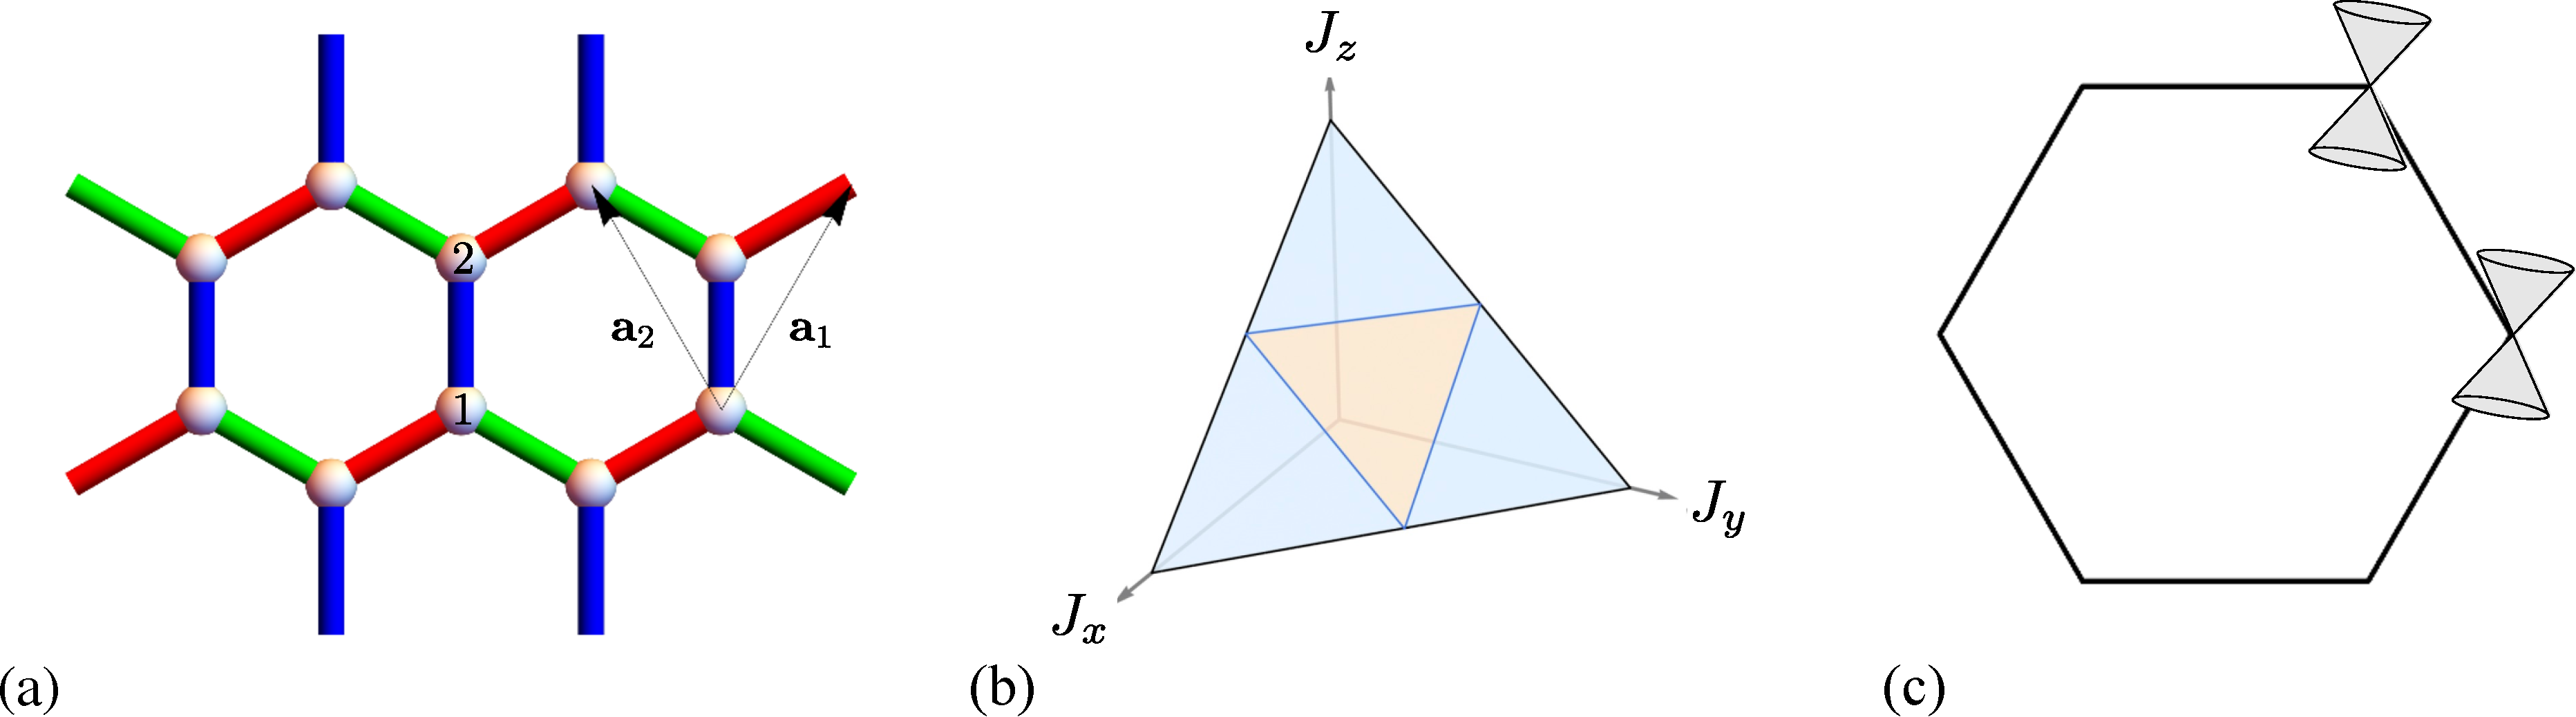
\includegraphics[width=\linewidth]{./chapter02/HoneycombPanel.pdf}
	\caption{
		(a) Unit cell and lattice vectors for the Kitaev model on the honeycomb lattice.
		Red, green and blue colored links correspond to $x$-, $y$- and $z$-type bonds, respectively.
		(b) Ground state phase diagram of the Kitaev model on the honeycomb lattice ($J_x + J_y + J_z = 1$).
		The blue regions correspond to gapped spin liquid phases, whereas the orange region corresponds to the gapless spin liquid phase.
		(c) Visualization of the Dirac cones for isotropic coupling.
	}
	\label{fig:chapter02_HoneycombPanel}
\end{figure}
%
The Kitaev model describes a system of interacting quantum spin-$1/2$ moments located at the vertices of a two-dimensional honeycomb lattice and is governed by the Hamiltonian
%
\begin{equation}
	\op{H}_{\rm Kitaev} = -J_x \sum_{x {\rm -links}} \sigma_j^x \sigma_k^x - J_y \sum_{y {\rm -links}} \sigma_j^y \sigma_k^y - J_z \sum_{z {\rm -links}} \sigma_j^z \sigma_k^z,
	\label{eq:chapter02_KitaevHamiltonian}
\end{equation}
%
where the summations are over nearest neighbor spins $\avg{j,k}$ with each link counted exactly once, the exchange couplings are chosen to be ferromagnetic, \ie, $J_{\gamma} \geq 0$, and each link connecting the spins is assigned to be of type $x$, $y$ or $z$.
The assignment of bond types is given in Figure~\ref{fig:chapter02_HoneycombPanel}~(a), where red, green and blue colored links correspond to $x$-, $y-$ and $z-$type bonds, respectively.
The Hamiltonian~\eqref{eq:chapter02_KitaevHamiltonian} may be written more compactly as
%
\begin{equation}
	\op{H}_{\rm Kitaev} = -\sum_{\gamma {\rm -links}} J_{\gamma}~\sigma_j^{\gamma} \sigma_k^{\gamma}.
	\label{eq:chapter02_KitaevHamiltonianCompact}
\end{equation}
%

The spins interact with their nearest neighbors via an Ising-like exchange, however, the component of the spin which is coupled depends on the type of bond connecting the neighboring spins.
This directional dependence of the exchange makes it impossible for a given spin to satisfy all of its neighbors simultaneously and results in a highly frustrated lattice of spins.
Despite describing a system of strongly interacting and highly frustrated quantum spins, the model is exactly solvable due to the combination of it possessing an extensive number of conserved quantities along with a clever representation of the Pauli matrices in terms of Majorana operators.

The first step to solving the model is the identification of conserved quantities.
For each hexagonal plaquette $p$ in the lattice, one may define a product of spins around the corresponding closed loop as
%
\begin{equation}
	\op{W}_p = -\prod_{\avg{j,k}\in p} \left(-i \sigma_j^{\gamma} \sigma_k^{\gamma}\right),
	\label{eq:chapter02_SpinLoopOperator}
\end{equation}
%
where the product is understood to occur in the counter-clockwise sense around the loop.
All such loop operators commute with each other as well as with the Hamiltonian~\eqref{eq:chapter02_KitaevHamiltonianCompact} and, thus, represent an extensive number of conserved quantities.
As such, they serve to partition the Hilbert space of the spins into sectors corresponding to the set of eigenvalues $\{w_p\}$.
The loop operators can be shown to be both Hermitian and unitary and, thus, have eigenvalues $w_p = \pm 1$.
These loop operators will later be seen to correspond to the fluxes of a \ZZ~gauge field and the eigenspaces $\{w_p\}$ will be referred to as "flux" sectors.

As the definition of the loop operator in Eq.~\eqref{eq:chapter02_SpinLoopOperator} differs from that usually encountered in the literature, note that it is chosen in order to maintain consistency when working with lattices other than the honeycomb.
The factors of $i$ act to ensure that the operator $\op{W}_p$ is Hermitian no matter the length of the plaquette, whereas the choice of minus signs will be seen in Section~\ref{section:chapter02_Z2GaugeTheory} to fix a consistent relationship with the fluxes of the aforementioned \ZZ~gauge theory.
Note that for a loop of even length, the loop operator is even under time-reversal, whereas for a loop of odd length, the loop operator is odd under time-reversal.
This implies that any fixed flux eigenstate of a Kitaev Hamiltonian defined on a \textit{non}-bipartite lattice spontaneously breaks time-reversal symmetry as it necessarily specifies the fluxes through plaquettes of odd length.

One can already identify some properties of the eigenstates of Hamiltonian~\eqref{eq:chapter02_KitaevHamiltonianCompact} from flux conservation.
Any spin component $\sigma_j^{\gamma}$ anti-commutes with exactly two loop operators.
This implies that the application of a spin operator mixes orthogonal flux sectors, resulting in a vanishing spin expectation value $\avg{\sigma_j^{\gamma}} = 0$ for all sites of the lattice.
This further implies that all two spin correlation functions must vanish unless the application of the second spin removes (reintroduces) the fluxes introduced (removed) by the first~\cite{BaskaranPRL2007}.
This happens only for on-site correlation functions and for nearest neighbor correlation functions of the form $\avg{\sigma_j^{\gamma} \sigma_k^{\gamma}}$, where sites $j, k$ are connected by a link of type $\gamma$.
These relations hold for \textit{all} eigenstates of the Hamiltonian.
Thus, the ground state of the Kitaev Hamiltonian~\eqref{eq:chapter02_KitaevHamiltonianCompact} has vanishing magnetization and (extremely) short-ranged spin-spin correlations as a quantum spin liquid should.


%
%
%%%%%%%%%%%%%%%%%%%%%%%%%%%%%%%%%%%%%%%%%%%%%%%%%%%%%%%%%%%%%%%%%%%%%%%%%%%%%%%%%%%%%%%%
\section{\texorpdfstring{\ZZ}{Z2}~gauge theory description}
\label{section:chapter02_Z2GaugeTheory}
%%%%%%%%%%%%%%%%%%%%%%%%%%%%%%%%%%%%%%%%%%%%%%%%%%%%%%%%%%%%%%%%%%%%%%%%%%%%%%%%%%%%%%%%
%
%
While the identification of conserved fluxes is a step in the right direction, it does not provide a complete solution to the problem.
In order to solve the model, it will be necessary to introduce an alternate representation of the spin-$1/2$ operators.
In this presentation, the solution originally introduced by Kitaev \cite{KitaevAoP2006} will be used.
There do exist, however, several other representations which have been used to solve this problem including Jordan-Wigner transformation \cite{FengPRL2007}, $SU(2)$ slave fermion representation \cite{BurnellPRB2011} as well as \textit{other} Majorana representations \cite{Tsvelik2003,YouPRB2012,SeifertPRBFeb2018,SeifertPRBOct2018} (as will be discussed in Chapter~\ref{chapter:ProjectiveSymmetryGroup}), each of which has its own strengths and weaknesses depending upon the desired application.

The approach used here will be to introduce four Majorana operators $c^{\gamma}$ at each site of the lattice, where $\gamma = 0,x,y,z$ (the superscript for $c^0$ will be dropped for notational convenience and readability wherever it does not hinder clarity).
These Majorana operators satisfy the usual Clifford algebra relations
%
\begin{equation}
	\{c_j^{\mu}, c_k^{\nu}\} = 2\delta^{\mu\nu}\delta_{jk}.
\end{equation}
%
Note that the Hilbert space of the Majorana operators at a given site is twice as large as that of the corresponding spin-$1/2$ operator.
One may introduce operators that act on this extended space
%
\begin{equation}
	\til{\sigma}_j^\mu = i c_j^{\mu} c_j \qquad (\mu = x,y,z)
	\label{eq:chapter02_ExtendedSpinOperators}
\end{equation}
%
which satisfy the same algebraic relations as the Pauli matrices \textit{when acting on physical states}.
The definition of extended spin-$1/2$ operators in Eq.~\eqref{eq:chapter02_ExtendedSpinOperators} is seen to possess a local \ZZ~gauge redundancy $c_j^\gamma \mapsto -c_j^\gamma$.
The physical Hilbert space is defined by those states satisfying $\op{D}_j = 1$ for all sites $j$, where the operator $\op{D}_j = c_j^x c_j^y c_j^z c_j$ represents the \ZZ~gauge transformation at site $j$, \ie,
%
\begin{equation}
	\{\op{D}_j, c_j^{\gamma}\} = 0.
\end{equation}
%

Replacing the spin operators of the original Hamiltonian~\eqref{eq:chapter02_KitaevHamiltonianCompact} with those in the extended space, one obtains a Hamiltonian of interacting Majorana fermions
%
\begin{equation}
	\op{H} = -\sum_{\avg{j,k}_{\gamma}} J_{\gamma}~(i c_j^{\gamma} c_j) (i c_k^{\gamma} c_k).
	\label{eq:chapter02_InteractingFermionHamiltonian}
\end{equation}
%
Defining link operators $\op{u}_{jk} = -\op{u}_{kj} = i c_j^{\gamma} c_k^{\gamma}$ on every link $\avg{j,k}_{\gamma}$, the Hamiltonian may be written\footnote{The $\dag$ has been included in the Hamiltonian in order to make the definition of the gauge transformations consistent.}
%
\begin{equation}
	\op{H} = i \sum_{\avg{j,k}_{\gamma}} J_{\gamma}~c\dag_j~\op{u}_{jk}~c_k
	\label{eq:chapter02_KitaevHamiltonianZ2}
\end{equation}
%
where it is easily seen to be invariant under local \ZZ~gauge transformations\linebreak $\op{G}_j \in \{\id_j,\op{D}_j\}$:
%
\begin{align}
	c_j &\rightarrow \op{G}_j c_j \nonumber\\
	\op{u}_{jk} &\rightarrow \op{G}_j \op{u}_{jk} \op{G}_k.
\end{align}
%
Of note is that the link operators commute with each other as well as with the Hamiltonian~\eqref{eq:chapter02_InteractingFermionHamiltonian} and represent conserved quantities.
Thus, they may serve to partition the extended Hilbert space into sectors corresponding to their eigenvalues $u_{jk}$.
As these operators are Hermitian and unitary, their eigenvalues $u_{jk} = \pm 1$.
Furthermore, replacing the spins in the definition of the loop operators $\op{W}_p$ to act in the extended space, one finds
%
\begin{align}
	\op{\til{W}}_p	&= -i^{|p|}\prod_{\avg{j,k}\in p} i \op{u}_{jk} \nonumber\\
				&= -i^{|p|} e^{i \op{\Phi}_p},
\end{align}
%
where $|p|$ denotes the length of the loop (for the honeycomb lattice considered here, $|p| = 6$) and $\op{\Phi}_p$ is the \ZZ-flux through the plaquette, establishing $\op{u}_{jk}$ as elements of a static \ZZ~gauge field where the loop operators $\op{W}_p$ correspond to the gauge-invariant fluxes of the gauge field.

In light of this interpretation, Hamiltonian~\eqref{eq:chapter02_KitaevHamiltonianZ2} may now be viewed as describing Majorana fermions hopping in the background of a static \ZZ~gauge field.
In principle, the \ZZ~gauge variables may be replaced by a static configuration and the resulting quadratic Hamiltonian diagonalized.
However, if one wishes to solve for the ground state, then the flux configuration of the ground state must first be determined.
Only then may a compatible gauge configuration be fixed and the Hamiltonian solved.


%
%
%%%%%%%%%%%%%%%%%%%%%%%%%%%%%%%%%%%%%%%%%%%%%%%%%%%%%%%%%%%%%%%%%%%%%%%%%%%%%%%%%%%%%%%%
\section{General aspects of the solution}
\label{section:chapter02_GeneralAspects}
%%%%%%%%%%%%%%%%%%%%%%%%%%%%%%%%%%%%%%%%%%%%%%%%%%%%%%%%%%%%%%%%%%%%%%%%%%%%%%%%%%%%%%%%
%
%
In order to solve for the ground state of Hamiltonian~\eqref{eq:chapter02_KitaevHamiltonianZ2}, one wishes to fix a gauge configuration and diagonalize the resulting quadratic Hamiltonian.
This gauge configuration must be constrained to yield the flux configuration of the ground state, making it necessary to first determine this ground state \textit{flux} configuration.
The most obvious way forward is a brute force numerical evaluation of possible flux configurations.
This, in fact, was the approach originally taken by Kitaev.

There is, however, a more efficient route available due to the work of Elliot Lieb and Michael Loss \cite{LiebHPA1992, LiebDMJ1993,LiebPRL1994,MacrisJSP1996}.
According to this work, for any \textit{elementary} loop $p$ in the lattice, \ie, a closed loop which cannot be formed by combining smaller loops, the flux $\Phi_p$ through the corresponding plaquette which minimizes the energy of the Hamiltonian takes the value
%
\begin{equation}
	\Phi_p = \pi(|p|-2)/2 \qquad ({\rm mod}~2\pi),
\end{equation}
%
where $|p|$ is the length of the elementary loop.
More concretely, this means that for $|p| = 0~({\rm mod}~4)$ the flux takes the value $\Phi_p = \pi$, whereas for $|p| = 2~({\rm mod}~4)$ the flux takes the value  $\Phi_p = 0$.
These two configurations shall be referred to as $\pi$-flux and $0$-flux, respectively.
A configuration of fluxes where \textit{every} elementary loop in the lattice takes such a minimizing value is known as a \textit{canonical flux configuration} \cite{MacrisJSP1996}.
Note that for a canonical flux configuration all loop operators have eigenvalue $w_p = +1$.
Furthermore, such a canonical flux configuration is guaranteed to exist for any $D$-dimensional bipartite lattice possessing a ($D-1$)-dimensional reflection hyperplane $P$ satisfying the following criteria:
%
\begin{enumerate}[label=(\alph*),leftmargin=3\parindent]
	\item $P$ does not intersect any vertices of the lattice,
	\item The whole lattice, along with the configuration of magnitudes of the hopping matrix elements of the Hamiltonian (in this case, the exchange couplings $J_{\gamma}$), is invariant under reflection through $P$,
	\item All elementary loops intersected by $P$ are invariant, up to orientation, under reflection through $P$.
\end{enumerate}
%

For the honeycomb lattice considered here, where $|p| = 6$ for all elementary loops, this corresponds to a ground state with uniform vanishing flux through all plaquettes.
Since, additionally, there exist such mirror planes $P$ for every plaquette in the lattice, one is guaranteed that such a canonical flux configuration exists.

Having determined the ground state flux sector to be the zero flux configuration, one is free to fix a compatible gauge configuration $\{u_{jk}\}$ resulting in a Hamiltonian which may be written as
%
\begin{equation}
	\op{H}(\{u_{jk}\}) = \frac{i}{4} \sum_{j,k} c_j A_{jk} c_k,
	\label{eq:chapter02_KitaevHamiltonianAMatrix}
\end{equation}
%
where $A$ is a skew-symmetric matrix with elements given by
%
\begin{equation}
	A_{jk} = \left\{
	\begin{matrix*}[l]
		2~J_{\gamma}~u_{jk} &
		\qquad \text{for $(j,k) \in \avg{j,k}_{\gamma}$}\\
		&\\
		0 &
		\qquad \text{otherwise,}
	\end{matrix*}
	\right.
\end{equation}
%
with the additional factor of $1/2$ accounting for the double counting of bonds.
The skew-symmetry of the matrix $iA$ is a manifestation of the particle-hole symmetry of the Majorana Hamiltonian due to the Majorana condition $c\dag = c$.
A consequence of this particle-hole symmetry is that all eigenvalues of $iA$ come in pairs $\epsilon_{\alpha}$ and $\epsilon_{\beta} = -\epsilon_{\alpha}$ corresponding to complex eigenvectors $\psi_{\alpha}$ and $\psi_{\beta} = \psi^*_{\alpha}$, respectively.
This implies that the complex fermionic creation and annihilation operators for such states $\alpha, \beta$ satisfy
%
\begin{equation}
	f\dag_{\alpha} = f_{\beta},
	\label{eq:chapter02_HalfFermionicStates}
\end{equation}
\ie, only half of the eigenstates of the Majorana Hamiltonian correspond to independent complex fermionic states.
The choice of which states correspond to creation operators and which correspond to annihilation operators is arbitrary up to the constraint in Eq.~\eqref{eq:chapter02_HalfFermionicStates}, and the most convenient choice depends on the desired application.
Having diagonalized the matrix $iA$ and chosen all creation operators to correspond to non-negative eigenvalues $\epsilon_{\alpha}$, one may write the Hamiltonian as
%
\begin{equation}
	\op{H} = \sum_{\alpha} \epsilon_{\alpha} \left(f\dag_{\alpha} f_{\alpha} - 1/2\right),
	\label{eq:chapter02_KitaevHamiltonianDiagonal}
\end{equation}
%
where $f\dag, f$ are usual complex fermionic creation and annihilation operators.
The ground state energy is now seen to be $E_0 = -\sum_{\alpha} \epsilon_{\alpha}/2$.

One can now see that the model possesses \textit{two} distinct types of fractionalized excitations: fluxes and fermions.
In Sec.~\ref{section:chapter02_Definition} it was shown that the application of a spin operator $\sigma_j^{\gamma}$ introduces (removes) pairs of fluxes.
Since the ground state flux configuration is by definition the lowest energy flux configuration, the insertion of flux pairs into the zero flux configuration yields eigenstates of \textit{higher} energy.
These \ZZ~flux excitations, or \textit{visons}, are gapped for any finite value of the exchange couplings $J_{\gamma}$.

From Eq.~\eqref{eq:chapter02_KitaevHamiltonianDiagonal}, one can see that, within the ground state flux sector (or any flux sector), the creation of a (complex) fermionic quasiparticle comes with an excitation energy $\epsilon_{\alpha}$.
These fermionic excitations may be gapped or gapless depending on the relative strengths of the exchange couplings and are the subject of the following section.


%
%
%%%%%%%%%%%%%%%%%%%%%%%%%%%%%%%%%%%%%%%%%%%%%%%%%%%%%%%%%%%%%%%%%%%%%%%%%%%%%%%%%%%%%%%%
\section{Ground state phase diagram}
\label{section:chapter02_GroundstatePhaseDiagram}
%%%%%%%%%%%%%%%%%%%%%%%%%%%%%%%%%%%%%%%%%%%%%%%%%%%%%%%%%%%%%%%%%%%%%%%%%%%%%%%%%%%%%%%%
%
%
Since the ground state flux configuration preserves the translation symmetry of the original spin Hamiltonian~\eqref{eq:chapter02_KitaevHamiltonian}, \ie, of the honeycomb lattice, a convenient choice for the gauge configuration is one which also preserves this symmetry.
For the case of the Kitaev model on the honeycomb lattice this is, indeed, possible (Chapter~\ref{chapter:ProjectiveSymmetryGroup} introduces the idea of gauge configurations having lower symmetry than the flux configuration).
One may then proceed by Fourier transforming the Hamiltonian~\eqref{eq:chapter02_KitaevHamiltonianAMatrix}.

Introducing Fourier transformed Majorana operators as
%
\begin{equation}
	c_j(\bk) = \frac{1}{\sqrt{2N}} \sum_{\br} e^{-i \bk\cdot\br} c_j(\br),
	\label{eq:chapter02_FourierMajorana}
\end{equation}
%
satisfying
%
\begin{equation}
	\{c_i(\bk), c_j(\bq)\} = \delta_{ij}\delta_{\bk,-\bq},
\end{equation}
%
where the summation in Eq.~\eqref{eq:chapter02_FourierMajorana} is over all unit cells, $N$ is the total number of unit cells, and the subscript $j$ refers to the site-index within a given unit cell (see Figure~\ref{fig:chapter02_HoneycombPanel}~(a)), one may write the Hamiltonian in momentum space as
%
\begin{equation}
	\op{H} = \sum_{\bk}
	\begin{pmatrix}
		c_1 (-\bk) &
		c_2 (-\bk)
	\end{pmatrix}
	\begin{pmatrix}
		0 &
		i f(\bk) \\
		&\\
		-i f^*(\bk) &
		0
	\end{pmatrix}
	\begin{pmatrix}
		c_1 (\bk) \\
		\\
		c_2 (\bk)
	\end{pmatrix},
\end{equation}
%
where
%
\begin{equation}
	f(\bk) = J_x e^{i \bk\cdot\ba_1} + J_y e^{i \bk\cdot\ba_2} + J_z.
\end{equation}
%
The eigenvalues of the momentum space Hamiltonian matrix are given by $\epsilon(\bk) = \pm |f(\bk)|$.

It can be shown that there are vanishing eigenvalues only for exchange couplings satisfying the triangle inequalities (see phase diagram in Figure~\ref{fig:chapter02_HoneycombPanel}~(b))
%
\begin{equation}
	|J_x| \leq |J_y| + |J_z|, \qquad |J_y| \leq |J_z| + |J_x|, \qquad |J_z| \leq |J_x| + |J_y|.
\end{equation}
%
Thus, for roughly isotropic couplings there exists a gapless spin liquid phase where, although the flux excitations remain gapped, the fermionic excitations are \textit{gapless}.
For highly anisotropic couplings, the system is in a fully gapped spin liquid phase which turns out to be equivalent to Kitaev's toric code model \cite{KitaevAoP2003,KitaevAoP2006} (see Appendix~\ref{appendix:LoopModels_6_3} for a derivation).

While in the gapless phase, the fermions exhibit a "graphene-like" band structure with two Dirac cones.
At the isotropic point ($J_x = J_y = J_z$), these Dirac cones are centered at the $K$ and $K'$ points in the Brillouin zone (see Figure~\ref{fig:chapter02_HoneycombPanel}~(c)) and have low-energy dispersion given by
%
\begin{equation}
	E(\mathbf{\delta k}) \approx v_{\alpha\beta} \sqrt{\delta k^{\alpha} \delta k^{\beta}},
\end{equation}
%
where $v_{\alpha\beta}$ corresponds to the Fermi velocity and $\mathbf{\delta k}$ is the displacement from the $K$ or $K'$ point, respectively.
As the exchange couplings are tuned away from this point, the Dirac cones move through the Brillouin zone, eventually meeting one another and mutually annihilating at the border between the gapless and gapped phases.


%
%
%%%%%%%%%%%%%%%%%%%%%%%%%%%%%%%%%%%%%%%%%%%%%%%%%%%%%%%%%%%%%%%%%%%%%%%%%%%%%%%%%%%%%%%%
\section{Application of a weak magnetic field}
\label{section:chapter02_WeakMagneticField}
%%%%%%%%%%%%%%%%%%%%%%%%%%%%%%%%%%%%%%%%%%%%%%%%%%%%%%%%%%%%%%%%%%%%%%%%%%%%%%%%%%%%%%%%
%
%
%%%%%%%%%%%%%%%%%%%%%%%%%%%%%%%%%%%%%%%%%%%%%%%%%%%%%%%%%%%%%%%%%%%%%%%%%%%%%%%%%%%%%%%%
\subsection{The significance of time-reversal symmetry}
%%%%%%%%%%%%%%%%%%%%%%%%%%%%%%%%%%%%%%%%%%%%%%%%%%%%%%%%%%%%%%%%%%%%%%%%%%%%%%%%%%%%%%%%
%
%
Before discussing the application of a weak magnetic field to the pure Kitaev model, it is instructive to understand the role which time-reversal symmetry plays in the system.
Particularly of interest is the way in which time-reversal symmetry is represented in the corresponding \ZZ~gauge theory of Majorana fermions and the physical repercussions thereof.

Physically, the time-reversal operator $\op{\mathcal{T}}$ acts on spins as
%
\begin{equation}
	\op{\mathcal{T}} \sigma_j^{\gamma} \op{\mathcal{T}}\inv = -\sigma_j^{\gamma}.
\end{equation}
%
The Kitaev Hamiltonian is obviously invariant under application of time-reversal.
Furthermore, there is no \textit{spontaneous} breaking of time-reversal symmetry as all eigenstates of the Kitaev Hamiltonian are also time-reversal invariant since
%
\begin{equation}
	\op{\mathcal{T}} \op{W}_p \op{\mathcal{T}}\inv = \op{W}_p
\end{equation}
%
due to the fact that the honeycomb lattice is bipartite, \ie, fixing a flux sector does not break time-reversal symmetry.

Naturally, the question arises: "Does fixing a \textit{gauge} sector preserve time-\linebreak reversal symmetry?"
In order to answer this question, it is necessary to understand how time-reversal acts on the Majorana operators.
Naively, one might ascribe the following simple behavior to the time-reversal operator in the Majorana sector
%
\begin{equation}
\op{\mathcal{T}} c_j^{\gamma} \op{\mathcal{T}}\inv = c_j^{\gamma}
\end{equation}
%
as it reproduces the physical action on the spins.
Unfortunately, such an operator will also act to reverse the sign of the gauge-fixed Hamiltonian (Eq.~\eqref{eq:chapter02_KitaevHamiltonianAMatrix}).
Thus, fixing a gauge sector appears to break time-reversal symmetry.

However, for certain lattices it is possible to define a physically equivalent operator $\op{\mathcal{T}}\prm$ which \textit{does} preserve time-reversal symmetry in a fixed gauge sector.
For a bipartite lattice, a gauge sector $\{u_{jk}\}$ and its time-reversal partner $\{-u_{jk}\}$ are gauge-equivalent.
The time-reversal operator may, thus, be "repaired" by being combined with the gauge transformation relating a gauge sector to its time-reversal partner.
The "repaired" or \textit{projective} time-reversal operator acts on the Majorana operators as
%
\begin{equation}
\op{\mathcal{T}}\prm c_j^{\gamma} \op{\mathcal{T}}^{\prime-1} = (-1)^{\zeta_j} c_j^{\gamma}
\end{equation}
%
where\footnote{An explicit convention for the bipartition of the lattice into sublattices $A$ and $B$ is not necessary as the desired result of the operator $\op{\mathcal{T}}\prm$ is achieved independent of which convention is used.}
%
\begin{equation}
	\zeta_j = \left\{
		\begin{matrix*}[l]
			0 &
			\qquad \text{for $j \in$ sublattice $A$} \\
			&\\
			1 &
			\qquad \text{for $j \in$ sublattice $B$},
		\end{matrix*}
		\right.
\end{equation}
%
thus, preserving the choice of gauge $\{u_{jk}\}$.
In principle, \textit{any} symmetry operator of the physical theory may require a similar projective representation in the extended space of the \ZZ~gauge theory in order to work within a fixed gauge sector.
This will turn out to be a powerful concept in the context of classifying certain quantum spin liquids and is the topic of Chapters~\ref{chapter:ProjectiveSymmetryGroup} and~\ref{chapter:ClassificationOfKSL}.

While gauge transformations are, of course, unphysical, the exact form of the gauge transformation required for the projective time-reversal symmetry operator \textit{does} have physical consequences for the nature of the fermionic excitations.
In a fixed gauge, the projective time-reversal operator (from here on, the prime symbol shall be omitted) may be represented as $\op{\mathcal{T}} = \op{G}_{\mathcal{T}} \op{K}$, where the unitary gauge transformation $\op{G}_{\mathcal{T}}$ simply represents a sublattice transformation satisfying
%
\begin{equation}
	\{\op{H}, \op{G}_\mathcal{T}\} = 0.
\end{equation}
%
In momentum space, this is is implemented as
%
\begin{equation}
	\op{\mathcal{T}} H(\bk) \op{\mathcal{T}}\inv = G_\mathcal{T} H^*(-\bk) G_\mathcal{T}\inv,
\end{equation}
%
where the sublattice transformation is represented explicitly as
%
\begin{equation}
	G_\mathcal{T} = \tau^z
\end{equation}
%
and where $\tau^z$ is a Pauli matrix acting on the band indices.

The presence of this sublattice relation is what allows one to write the Hamiltonian matrix in off-diagonal form as
%
\begin{equation}
	H(\bk) = -\mathfrak{Im}[f(\bk)] \tau^x - \mathfrak{Re}[f(\bk)] \tau^y,
\end{equation}
%
where $\mathfrak{Re}[f(\bk)]$ and $\mathfrak{Im}[f(\bk)]$ are the real and imaginary parts of $f(\bk)$, respectively, satisfying $\mathfrak{Re}[f(-\bk)] = \mathfrak{Re}[f(\bk)]$ and $\mathfrak{Im}[f(-\bk)] = -\mathfrak{Im}[f(\bk)]$.
In general, zero energy fermionic excitations exist if and only if the determinant of the matrix $H(\bk)$ vanish for some real value(s) of crystal momentum $\bk$.
With the Hamiltonian written in off-diagonal form, \ie, in the basis which diagonalizes the sublattice transformation, one may see that the vanishing of the determinant is equivalent to the simultaneous vanishing of the real and imaginary parts of the function $f(\bk)$,
%
\begin{equation}
	\mathfrak{Re}[f(\bk)] = 0 \qquad\text{and}\qquad \mathfrak{Im}[f(\bk)] = 0.
	\label{eq:chapter02_DetHEqualsZero}
\end{equation}
%
In two spatial dimensions, this implies the need to tune two components of momentum such that two independent functions vanish simultaneously.
The result is that the only \textit{stable} zero modes possible in the system correspond to isolated points, \ie, Dirac nodes.

For a general $2\times2$ Hamiltonian, this sublattice "symmetry" can be broken by introducing a term proportional to either the identity $\id_{2\times2}$ or to $G_\mathcal{T} = \tau^z$.
The former represents an on-site potential and is not allowed for Majorana fermions, however, the latter could be realized by, \eg, the addition of hopping between next-nearest neighbors.
The addition of such a mass term $\Delta(\bk) \tau^z$ would result in the immediate gapping out of the Dirac nodes as it spoils the relation of Eq.~\eqref{eq:chapter02_DetHEqualsZero}.
As this sublattice relation is necessary for the definition of a projective time-reversal operator, such a mass term represents the breaking of time-reversal symmetry, implying that time-reversal symmetry of the physical spin Hamiltonian (as well as in the flux sectors) is required to stabilize the presence of fermionic zero modes.


%
%
%%%%%%%%%%%%%%%%%%%%%%%%%%%%%%%%%%%%%%%%%%%%%%%%%%%%%%%%%%%%%%%%%%%%%%%%%%%%%%%%%%%%%%%%
\subsection{Derivation of an effective Hamiltonian}
%%%%%%%%%%%%%%%%%%%%%%%%%%%%%%%%%%%%%%%%%%%%%%%%%%%%%%%%%%%%%%%%%%%%%%%%%%%%%%%%%%%%%%%%
%
%
Having understood the significance of time-reversal symmetry for the fermionic quasiparticle spectrum, an effective Hamiltonian for small magnetic fields\linebreak ${\bf h} = (h_x, h_y, h_z)$ will now be derived, representing a concrete, physical mechanism for the breaking of time-reversal symmetry.
The following is an expanded version of what appears in~\cite{KitaevAoP2006}.
The spins are coupled to the magnetic field as
%
\begin{equation}
	\op{H} = \op{H}_0 - \sum_j {\bf h} \cdot \bsigma_j,
\end{equation}
%
where $\op{H}_0$ denotes the pure Kitaev Hamiltonian.
In the following, isotropic exchange couplings $J_x = J_y = J_z = J$ are assumed, the magnetic field is understood to be small enough not to excite the gapped flux excitations of the gauge field, and all components of the magnetic field are to be positive.

The application of a magnetic field spoils the exact solvability of the Hamiltonian as it makes the fluxes dynamic.
However, a sufficiently small magnetic field may be treated perturbatively within the ground state flux sector.
An effective Hamiltonian $\op{H}_{\rm eff} = \op{H}_0 + \op{\Sigma}(E_0)$, where $E_0$ is the ground state energy of the unperturbed Hamiltonian, can be arrived at by solving for the self-energy
%
\begin{equation}
\op{\Sigma}(E_0) = \op{\Pi}_0 \big(\op{V} + \op{V} \op{G}'_0(E_0) \op{V} + \op{V} \op{G}'_0(E_0) \op{V} \op{G}'_0(E_0) \op{V} + \ldots~\big) \op{\Pi}_0.
\end{equation}
%
Here, $\op{V}$ is the coupling to the magnetic field, $\op{\Pi}_0$ is the projector to the ground state flux sector, and $G'_0$ is the Green's function of the unperturbed Hamiltonian with the prime indicating that it vanishes on ground states.

The first-order contribution to the self-energy vanishes as it maps to states outside of the ground state flux sector.
This can easily be seen by noting that the spin operator $\sigma^\gamma_j$ anti-commutes with any flux operator $\op{W}_p$ for which that spin is a part of the corresponding plaquette $p$.

At second order, the self-energy simply consists of constant terms corresponding to repeated application of the operator $\sigma_j^\gamma$, and non-constant terms proportional to the operators $\sigma_j^\gamma \sigma_k^\gamma$, where sites $j$ and $k$ are nearest neighbors connected by a $\gamma$-link.
The non-constant terms simply renormalize the hopping amplitudes of the Majorana operators and do not break time-reversal symmetry.

The first non-trivial contribution comes at third order with terms proportional to operators of the form $\sigma_i^\alpha \sigma_j^\beta \sigma_k^\gamma$ with $\alpha$, $\beta$ and $\gamma$ strictly not equal and the sites $j$, $k$ and $l$ arranged as in Figure~\ref{fig:chapter02_ThreeSpinTerms}.
The correct spin components $\alpha,\beta,\gamma$ for the specific examples of three-spin terms exhibited in Figure~\ref{fig:chapter02_ThreeSpinTerms} are denoted in the caption for that figure and should be understood to generalize in such a way that the overall change in flux is always vanishing.
Terms corresponding to the type shown in Figure~\ref{fig:chapter02_ThreeSpinTerms} (b) may be written as four-fermion terms in the Majorana operators
%
\begin{equation}
	\op{\Sigma}_{\rm (b)} \propto \sum_{(i,j,k)} i \epsilon^{\alpha\beta\gamma} \op{D}_l \op{u}_{li} \op{u}_{lj} \op{u}_{lk} c_i c_j c_k c_l,
\end{equation}
%
where $l$ denotes the common nearest neighbor of sites $i,j$ and $k$.
Such interactions have been shown to be RG irrelevant for Fermi surfaces with codimension $\geq 2$~\cite{HermannsPRL2015}.
As that is the case for Dirac fermions in 2D, these terms will be ignored here.
%
\begin{figure}[tb]
	\centering
	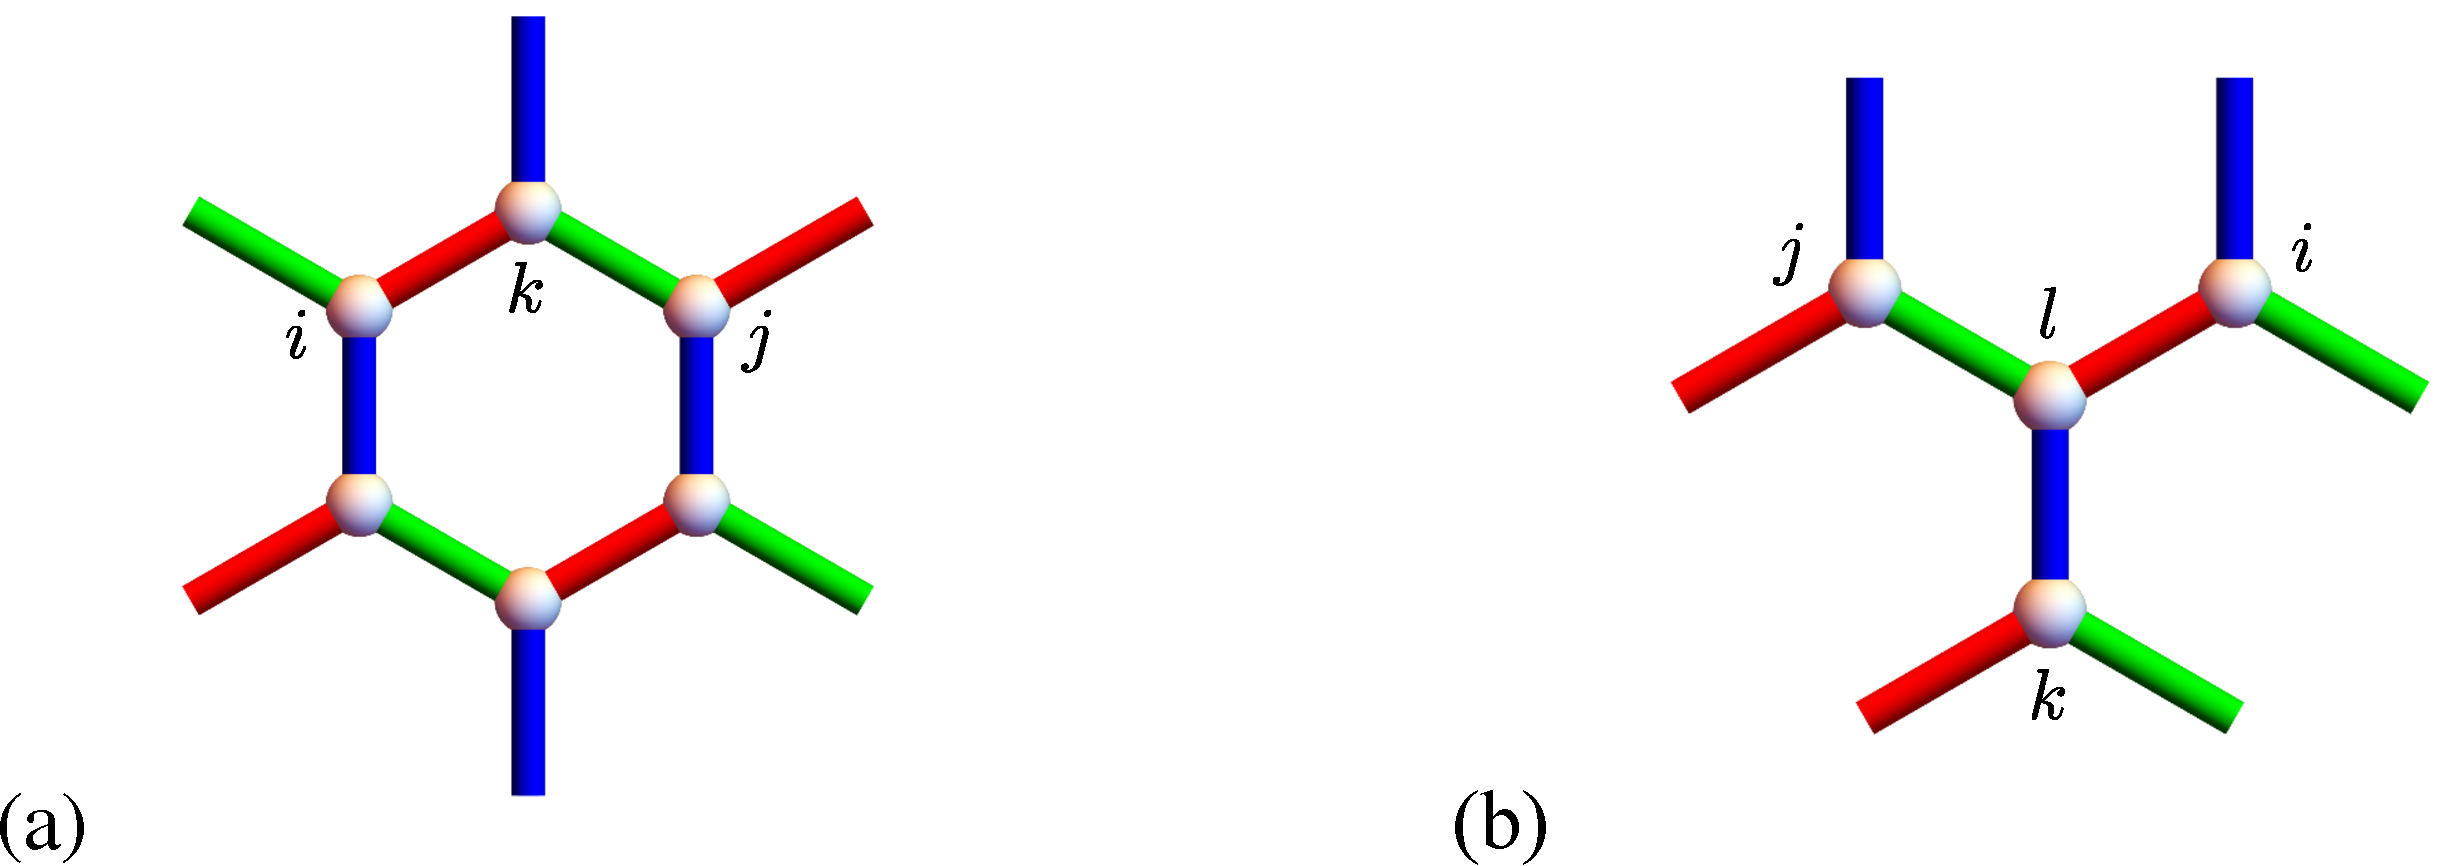
\includegraphics[width=0.8\linewidth]{./chapter02/ThreeSpinTerms.pdf}
	\caption{
		Graphical representation of third-order perturbation theory terms for the Kitaev Hamiltonian with an applied magnetic field.
		(a) Representation of the three-spin term $\sigma_i^x \sigma_j^y \sigma_k^z$ resulting in a next-nearest neighbor fermion hopping term.
		(b) Representation of the three-spin term $\sigma_i^x \sigma_j^y \sigma_k^z$ resulting in a four-fermion interaction term.
	}
	\label{fig:chapter02_ThreeSpinTerms}
\end{figure}
%

The remaining terms in Figure~\ref{fig:chapter02_ThreeSpinTerms} (a) may be reduced to Majorana bilinears resulting in next-nearest-neighbor hopping terms
%
\begin{equation}
	\op{\Sigma}_{\rm (a)} = \sum_{(i,j,k)} i \kappa \epsilon^{\alpha\beta\gamma} \op{D}_k \op{u}_{ik} \op{u}_{kj} c_i c_j,
	\label{eq:chapter02_HeffGauge}
\end{equation}
%
where the sum is over unordered triples $(i,j,k)$ of the type appearing in Figure~\ref{fig:chapter02_ThreeSpinTerms} (a) and where the intra-sublattice hopping strength $\kappa \sim \frac{h_x h_y h_z}{J^2}$ is determined by virtual flux excitations.
More precisely, $\kappa \approx 6\frac{h_x h_y h_z}{(0.27 J)^2}$ for the case presented here\footnote{The factor of $6$ is a combinatorial prefactor accounting for the fact that the sum in Eq.~\eqref{eq:chapter02_HeffGauge} occurs over \textit{unordered} triples.} on the honeycomb lattice~\cite{KitaevAoP2006}, however, the energy cost of virtual flux excitations depends on the lattice under consideration and the exact way in which the fluxes are excited~\cite{OBrienPRB2016}, as is shown in Chapter~\ref{chapter:ClassificationOfKSL} where generalizations of the Kitaev honeycomb model to other lattices are treated.

While the effective Hamiltonian~\eqref{eq:chapter02_HeffGauge} can be seen to mix different gauge sectors, as one wishes to work in the physical, \ie, gauge symmetrized, space, it shall henceforth be restricted to a fixed gauge.
Again choosing a translationally invariant gauge, the full Hamiltonian may be written in momentum space as
%
\begin{equation}
	H(\bk) = -\mathfrak{Im}[f(\bk)] \tau^x - \mathfrak{Re}[f(\bk)] \tau^y + \Delta(\bk) \tau^z,
	\label{eq:chapter02_KitaevHamiltonianMagnetic}
\end{equation}
%
where the mass term is given by
%
\begin{equation}
	\Delta(\bk) = 4\kappa \big(\sin{(\bk \cdot \ba_1)} - \sin{(\bk \cdot \ba_2)} + \sin{(\bk \cdot (\ba_1 - \ba_2))}\big).
\end{equation}
%
Here it can be seen how the breaking of time-reversal symmetry in physical spin space lead to the breaking of time-reversal symmetry in the fermionic Hamiltonian, signaled concretely by the breaking of sublattice symmetry.
The resulting dispersion of the fermionic excitations in the presence of a magnetic field
%
\begin{equation}
	E(\bk) = \pm \sqrt{|f(\bk)|^2 + |\Delta(\bk)|^2}
\end{equation}
%
is now seen to posses an energy gap of $2\Delta(\bk^*)$, where $\bk^*$ corresponds to the momentum at which a Dirac node was located before the application of the magnetic field.


%
%
%%%%%%%%%%%%%%%%%%%%%%%%%%%%%%%%%%%%%%%%%%%%%%%%%%%%%%%%%%%%%%%%%%%%%%%%%%%%%%%%%%%%%%%%
\subsection{Topology of the effective Hamiltonian}
%%%%%%%%%%%%%%%%%%%%%%%%%%%%%%%%%%%%%%%%%%%%%%%%%%%%%%%%%%%%%%%%%%%%%%%%%%%%%%%%%%%%%%%%
%
%
%
\begin{figure}[tb]
	\centering
	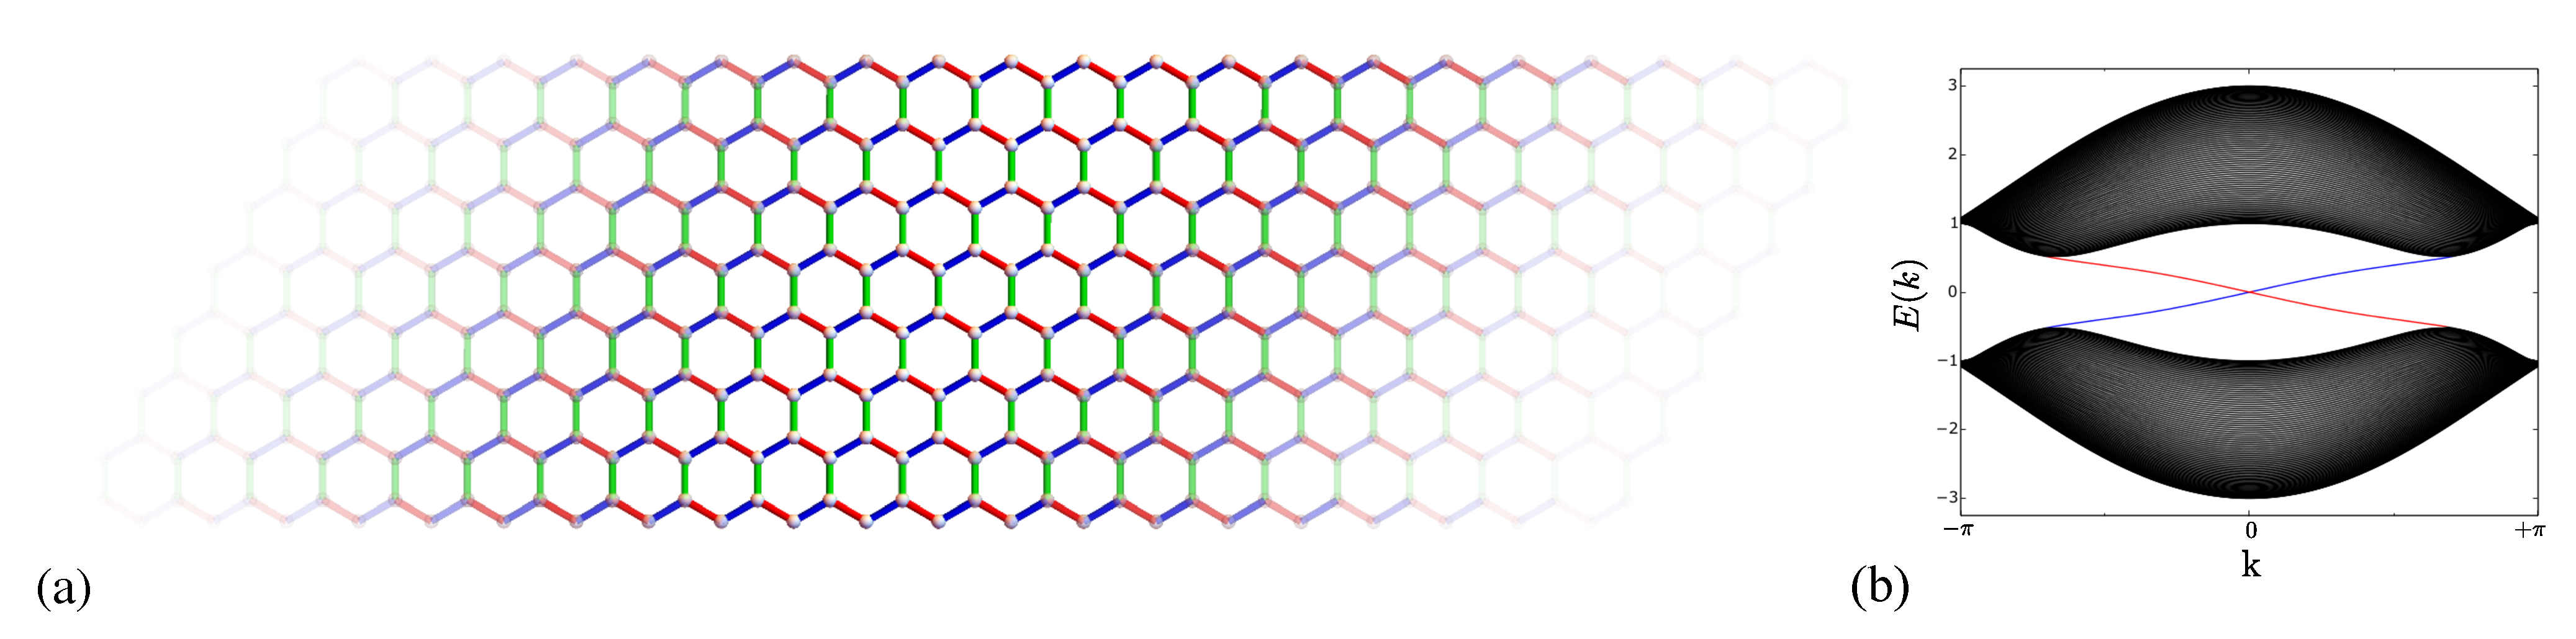
\includegraphics[width=\linewidth]{./chapter02/ChiralEdgeModes.pdf}
	\caption{
		(a) Example slab geometry with open boundary conditions in the $\ba_2$ direction.
		(b) Spectrum of the effective Hamiltonian~\eqref{eq:chapter02_HeffGauge} for a weak magnetic field on a slab geometry.
		The fully gapped bulk bands are depicted in black.
		The left- and right-moving chiral edge modes, depicted in red and blue, respectively, are localized to opposite edges of the sample and are due to the non-trivial topology of the band structure signaled by a non-vanishing first Chern number.
	}
	\label{fig:chapter02_EdgeModes}
\end{figure}
%
When framed as a free fermion Hamiltonian, the pure Kitaev model on the honeycomb lattice corresponds to a Hamiltonian matrix in the Altland-Zirnbauer symmetry class BDI~\cite{ZirnbauerJMP1996,AltlandPRB1997}.
In this context, symmetry class BDI is defined as the class of all Hamiltonian matrices possessing time-reversal symmetry, particle-hole symmetry and sublattice symmetry, such that the time-reversal and particle-hole operators both square to the positive identity operator.
Free fermion Hamiltonians belonging to symmetry class BDI are well known to be topologically trivial in two dimensions~\cite{KitaevAIP2009,RyuNJP2010,WenPRB2012}.

However, having now simultaneously broken both time-reversal and sublattice symmetries while retaining particle-hole symmetry (squaring to $+\id$), the resulting free fermion Hamiltonian resides in symmetry class D.
Gapped free fermion Hamiltonians belonging to symmetry class D in two dimensions may be identified by an integer topological invariant known as the first Chern number~\cite{KitaevAIP2009,RyuNJP2010,WenPRB2012} (often shortened to just "Chern number" in this context).
The Chern number corresponds to the quantized total amount of Berry flux through the Brillouin zone and is well known to be an important quantity in the theory of the integer quantum Hall effect~\cite{ThoulessPRL1982,AvronPRL1983,BellissardJMP1994}.
It may be calculated directly from the eigenstates of the Hamiltonian as, \eg,
%
\begin{equation}
	\nu = \frac{1}{2\pi i} \int_{BZ} \trace{(P~dP \wedge dP)},
\end{equation}
%
where $P$ is the projector onto the negative energy states and the integral is over the entire first Brillouin zone.

The negative energy band of Hamiltonian~\eqref{eq:chapter02_KitaevHamiltonianMagnetic} can be shown to have a non-vanishing Chern number $\nu = 1$, distinguishing it as a topological Chern insulator rather than a trivial band insulator.
An observable consequence of this non-trivial topology is the existence of $\nu$ chiral gapless edge modes~\cite{HalperinPRB1982,HatsugaiPRL1993,SchulzBaldesJPA2000,KellendonkRMaP2002} (see Figure~\ref{fig:chapter02_EdgeModes}).
As will be discussed in Chapter~\ref{chapter:TransitionMetalOxides}, the Kitaev Hamiltonian may be viewed as an effective Hamiltonian of a Mott insulator and contains no electric charge carrying degrees of freedom, however, the chiral edge modes can carry a \textit{thermal} Hall current
%
\begin{equation}
	I = \frac{\pi}{24} \nu T^2
\end{equation}
%
for a small temperature gradient $T$ applied perpendicular to the sample's surface~\cite{KanePRB1997,CapelliNPB2002,KitaevAoP2006}.

Another consequence of the non-trivial topology is the presence of non-Abelian anyon excitations.
The non-Abelian statistics is due to the fact that, for non-\linebreak vanishing Chern number $\nu$, \ZZ~flux excitations carry a single, unpaired Majorana mode~\cite{KitaevAoP2006,LahtinenAoP2008}.


%
%
%%%%%%%%%%%%%%%%%%%%%%%%%%%%%%%%%%%%%%%%%%%%%%%%%%%%%%%%%%%%%%%%%%%%%%%%%%%%%%%%%%%%%%%%
\section{Summary}
\label{section:chapter02_Summary}
%%%%%%%%%%%%%%%%%%%%%%%%%%%%%%%%%%%%%%%%%%%%%%%%%%%%%%%%%%%%%%%%%%%%%%%%%%%%%%%%%%%%%%%%
%
%
Section~\ref{section:chapter02_Definition} introduces Kitaev's honeycomb model of interacting quantum spins and identifies a macroscopic number of conserved quantities defined by certain products of spins around the hexagonal plaquettes of the lattice.
In Section~\ref{section:chapter02_Z2GaugeTheory}, a representation of the spins in terms of Majorana operators is used to reframe the model as a theory of Majorana fermions coupled to a static \ZZ~gauge field.
The conserved quantities in Section~\ref{section:chapter02_Definition} are seen to correspond to the gauge fluxes in the Majorana representation and allow for an exact solution of the model.
Section~\ref{section:chapter02_GeneralAspects} discusses some general aspects of the solution including how to use Lieb's theorem to fix the ground state flux sector.
The full solution to the model is carried out in Section~\ref{section:chapter02_GroundstatePhaseDiagram}, establishing a ground state phase diagram which exhibits both gapped and gapless quantum spin liquid ground states.
While the gapped spin liquid phase is not discussed in detail in this work, the latter is seen to possess gapless fermionic excitations with a graphene-like dispersion.
In Section~\ref{section:chapter02_WeakMagneticField}, the effects of time-reversal symmetry breaking are explored both in general and in particular using a weak external magnetic field.
The Dirac fermions of the gapless phase are seen to be protected by the presence of time-reversal symmetry and are gapped out by an infinitesimal magnetic field, resulting in a topological Chern insulator.

In Chapter~\ref{chapter:ClassificationOfKSL}, Kitaev's honeycomb model is extended to a number of tricoordinated lattices in three-dimensions.
The tricoordination of these lattices ensures that an exact solution is possible, just as in the case of the two-dimensional honeycomb lattice discussed above.
Analogous to the original model, the Kitaev models defined on these lattices similarly exhibit both gapped and gapless spin liquid ground states.
The gapless fermionic excitations in these systems are seen to be very diverse, depending intimately on the geometry of a given lattice.
Chapter~\ref{chapter:ProjectiveSymmetryGroup} introduces an object called the \textit{projective symmetry group} in order to better understand the hidden order of quantum phases such as the spin liquid phase seen, \eg, in the Kitaev honeycomb model.
These ideas are shown to provide an understanding of the appearance and stability of these excitations in both the two- and three-dimensional Kitaev models.	% Kitaev Honeycomb Model
%%%%%%%%%%%%%%%%%%%%%%%%%%%%%%%%%%%%%%%%%%%%%%%%%%%%%%%%%%%%%%%%%%%%%%%%%%%%%%%%%%%%%%%%
\chapter[Transition Metal Oxides as Kitaev Materials]{Transition Metal Oxides as\linebreak Kitaev Materials}
\label{chapter:TransitionMetalOxides}
%%%%%%%%%%%%%%%%%%%%%%%%%%%%%%%%%%%%%%%%%%%%%%%%%%%%%%%%%%%%%%%%%%%%%%%%%%%%%%%%%%%%%%%%
%
%
Just a few years after Kitaev introduced his exactly solvable honeycomb model, Jackeli and Khaliullin had proposed a physical realization of the model in certain strongly spin-orbit coupled Mott insulators~\cite{JackeliPRL2009}.
In particular, they proposed that $A_2MO_3$ compounds, where $A$ and $M$ are alkali and late transition metal ions, respectively, could realize Kitaev exchange between local $j_{\rm eff} = 1/2$ moments for a certain arrangement of the ligand oxygen ions.

In such a material, the transition metal cations are surrounded by an octahedral cage of oxygen anions.
The crystal electric field resulting from the oxygens splits the degeneracy of the transition metal's partially filled $d$ subshell into an empty high-energy $e_g$ manifold and a low-energy $t_{2g}$ manifold with a single hole.
As the transition metal ions are quite massive, strong spin-orbit coupling further splits the degeneracy of the $t_{2g}$ bands, ultimately yielding a spin-orbit entangled $j_{\rm eff} = 1/2$ moment.
Although the $4d$ and $5d$ orbitals of the transition metal ions are rather extended resulting in a relatively weak on-site Coulomb repulsion, the narrow bandwidth of the $j_{\rm eff} = 1/2$ doublet allows for the formation of a so-called spin-orbit assisted Mott insulator.
Jackeli and Khaliullin showed that for idealized edge-sharing octahedra with inversion symmetry, the superexchange between the transition metal ions due to the oxygen ligands is precisely the Kitaev interaction.

This realization spawned an intense effort to find such Kitaev materials in the laboratory.
While a number of honeycomb materials -- as well as a number of \textit{three-dimensional} variants -- have been found to harbor dominant Kitaev interactions, all of these materials have been observed to exhibit long-range magnetic order at finite temperatures due to the presence of additional exchange interactions.
Despite the observation of magnetic order, it has been argued that at least one of these materials is \textit{proximate} to a Kitaev spin liquid phase and that evidence of fractionalization is seen to occur in certain thermodynamic signatures -- a claim which remains controversial.
The discovery of three-dimensional Kitaev materials has sparked much theoretical interest in three-dimensional Kitaev spin liquids, including the work reported in this thesis.

The remainder of this chapter is structured as follows.
Section~\ref{section:chapter03_CFSO} gives a detailed description of the mechanism by which the spin-orbit assisted Mott insulator forms in the transition metal oxides.
The superexchange mechanism leading to the Kitaev interaction is treated in Section~\ref{section:chapter03_SpinExchange}.
Inclusion of additional exchange interactions is also discussed in this section.
A brief overview of some prominent Kitaev materials in both two- and three-dimensions is given in Section~\ref{section:chapter03_Materials}.
Finally, Section~\ref{section:chapter03_Summary} provides a brief summary.


%
%
%%%%%%%%%%%%%%%%%%%%%%%%%%%%%%%%%%%%%%%%%%%%%%%%%%%%%%%%%%%%%%%%%%%%%%%%%%%%%%%%%%%%%%%%
\section{Spin-orbit entangled \texorpdfstring{$J_{\rm eff} = 1/2$}{Jeff=1/2}~Mott insulators}
\label{section:chapter03_CFSO}
%%%%%%%%%%%%%%%%%%%%%%%%%%%%%%%%%%%%%%%%%%%%%%%%%%%%%%%%%%%%%%%%%%%%%%%%%%%%%%%%%%%%%%%%
%
%
%
\begin{figure}[tb]
	\centering
	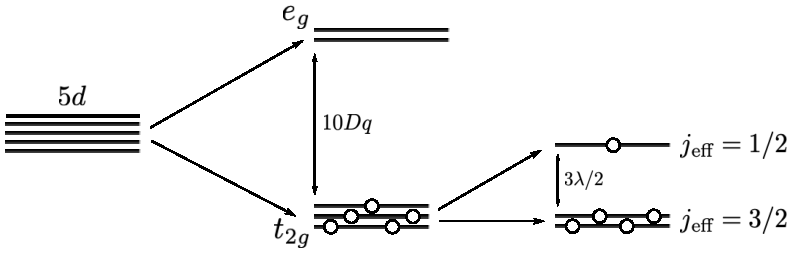
\includegraphics[width=\linewidth]{./chapter03/LevelSplitting.pdf}
	\caption{
		Splitting of $5d$ orbitals by crystal electric field and spin-orbit coupling resulting in $j_{\rm eff} = 1/2$ moment.
	}
	\label{fig:chapter03_LevelSplitting}
\end{figure}
%
In a spherically symmetric potential and without considering the relativistic effect of spin-orbit coupling, the state of an electron in an isolated atom or ion is characterized by the principle quantum number $n = 1, 2, \ldots$, the azimuthal quantum number $l = 0, 1, \ldots, n - 1$, the corresponding magnetic quantum number $m_l \in \{-l, -l+1, \ldots, l\}$ and the electron spin $m_s = \pm 1$, \ie,
%
\begin{equation}
	\ket{\psi_{\rm el}} = \ket{n, l, m_l, m_s}.
\end{equation}
%
Whereas the principle quantum number $n$ dictates the spatial extent of the electronic wave function -- with larger $n$ corresponding to a more delocalized electron -- $l$ and $m_l$ determine the orbital angular momentum and govern the shape of the wave function.
Different values of the orbital angular momentum $l$ correspond to \textit{subshells} of the $n^{\rm th}$ \textit{shell} and the different values of the magnetic quantum number $m_l$ correspond to the different \textit{orbitals}.
The orbitals in a subshell are commonly referred to as $s$-, $p$-, $d$-, or $f$-orbitals, corresponding to orbital angular momentum $l=0, 1, 2, 3$, respectively.
Beyond $l = 3$ the naming continues alphabetically with the exception that there are no $j$-orbitals.
For fixed values of $n$ and $l$, there are a total of $2 \times (2l + 1)$ degenerate states corresponding to the $2l + 1$ allowed values of the magnetic quantum number $m_l$ and the two possible values of the electron spin $m_s$.

This section will discuss the partial lifting of this degeneracy in the context of certain iridate compounds via anisotropic electric potentials -- the so-called \textit{crystal field} -- and by spin-orbit coupling.
For the case of five electrons in a partially filled $d$ subshell, it will be shown that the resulting low-energy description is that of an effective spin-1/2 moment (see Figure~\ref{fig:chapter03_LevelSplitting}).
Furthermore, electronic correlations are seen to localize the effective spin-1/2 degrees of freedom in a Mott insulating state.


%
%
\subsection{Crystal field splitting}
%
%
%
\begin{figure}[tb]
	\centering
	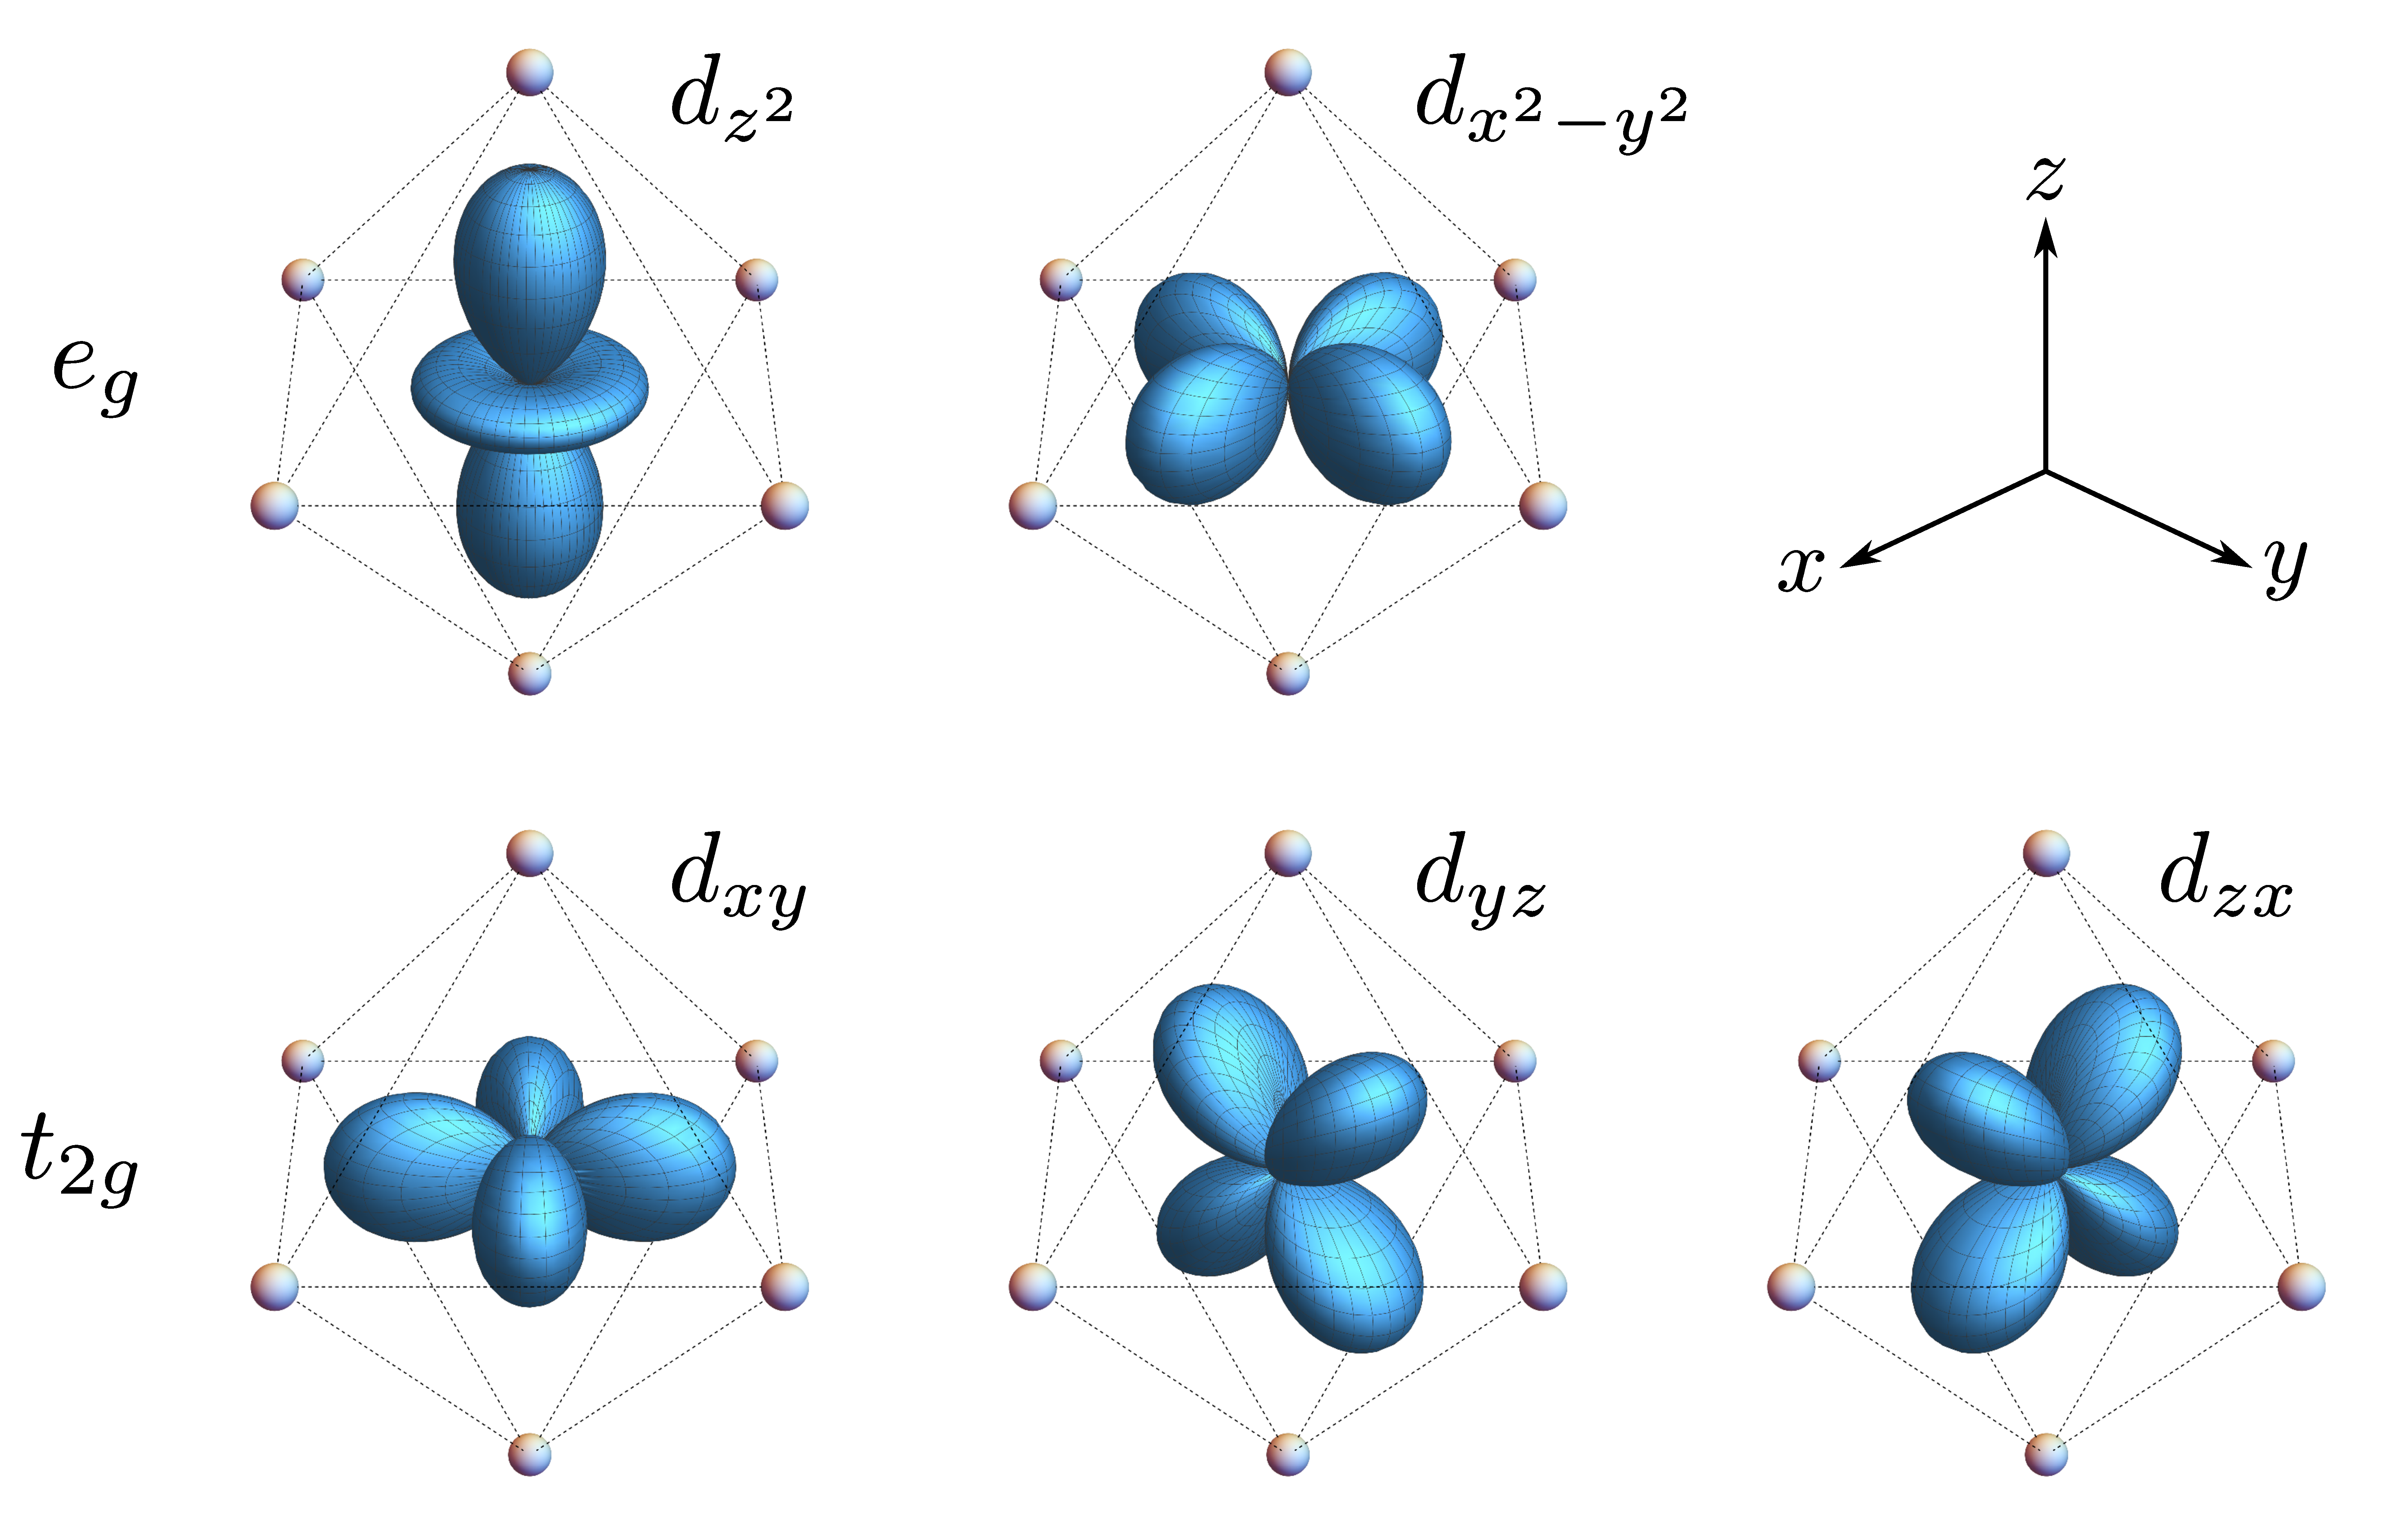
\includegraphics[width=\linewidth]{./chapter03/IridiumOrbitals.pdf}
	\caption{
		Higher energy $e_g$ and lower energy $t_{2g}$ orbitals of a transition metal cation in the center of an octahedral cage of ligand oxygen anions.
		The lobes of the $e_g$ orbitals are extended \textit{toward} the oxygen ligands, whereas the lobes of the $t_{2g}$ orbitals lie \textit{between} the ligands.
	}
	\label{fig:chapter03_SpatialOrbitals}
\end{figure}
%
In, \eg, the iridate materials Ir$^{4+}$ cations are surrounded by an octahedral cage of ligand O$^{2-}$ anions (see Figure~\ref{fig:chapter03_SpatialOrbitals}).
The resulting crystal electric field experienced by the electrons in the iridium atom, thus, exhibits a cubic symmetry.
As the orbital angular momentum determines the shape of the wave function, the cubic anisotropy naturally leads to a splitting of the orbital degeneracy.

In the case of the iridates, the iridium ions have a partially filled 5$d$-subshell.
The $d$-orbitals in an isolated ion have a fivefold degeneracy and may be specified by their total orbital angular momentum $l = 2$ along with their magnetic quantum number $m_l \in \{ 0, \pm 1, \pm 2 \}$ as $\ket{l, m_l}$ (suppressing the principle and spin quantum numbers).
The interaction of the $d$-electrons with the surrounding ions in the crystal, however, leads to a splitting of this degeneracy known as \textit{crystal field splitting}.
The $d$-orbitals are split into a lower-energy $t_{2g}$ triplet and a higher-energy $e_g$ doublet given by~\cite{Ballhausen1962,Griffith1971}
%
\begin{align}
	\begin{matrix*}[l]
		\begin{matrix*}[l]
			\ket{z^2}			\\
			\ket{x^2 - y^2}		
		\end{matrix*}
		&
		\begin{matrix*}[l]
			= \\
			=
		\end{matrix*}
		&
		\begin{matrix*}[l]
			\ket{2, 0} \\
			\frac{1}{\sqrt{2}} (\ket{2, 2} + \ket{2, -2})
		\end{matrix*}
		&
		\left.
		\begin{matrix*}[l]
			\\ \\
		\end{matrix*}
		\right\}~e_g~{\rm orbitals} \nonumber\\
		\nonumber\\
		\begin{matrix*}[l]
			\ket{xy}	\\
			\ket{yz}	\\
			\ket{zx}	
		\end{matrix*}
		&
		\begin{matrix*}[l]
			= \\
			= \\
			=
		\end{matrix*}
		&
		\begin{matrix*}[l]
			-\frac{i}{\sqrt{2}} (\ket{2, 2} - \ket{2, -2}) \\
			\phantom{-}\frac{i}{\sqrt{2}} (\ket{2, 1} + \ket{2, -1}) \\
			-\frac{1}{\sqrt{2}} (\ket{2, 1} - \ket{2, -1})
		\end{matrix*}
		&
		\left.
		\begin{matrix*}[l]
			\\ \\ \\
		\end{matrix*}
		\right\}~t_{2g}~{\rm orbitals}.
	\end{matrix*}
\end{align}
%

Referring to the above orbitals pictured in Figure~\ref{fig:chapter03_SpatialOrbitals}, one can understand this splitting from a purely geometric perspective.
Whereas the lobes of the $e_g$ orbitals are extended \textit{toward} the oxygen ligands, the lobes of the $t_{2g}$ orbitals lie \textit{between} the ligands.
The Coulomb interaction, thus, works to raise the energy of the $e_g$ orbitals relative to the $t_{2g}$ orbitals.
This contribution to the crystal field splitting is known as the \textit{point charge contribution}.
Additionally, one should consider the effects of hybridization of the $d$-orbitals of the iridium ions with the $p$-orbitals of the surrounding ligands.
Such hybridization is stronger for the $e_g$ orbitals than for the $t_{2g}$ orbitals, resulting in a level splitting.
Although the splitting due to hybridization tends to be stronger than the point charge contribution, they both result in the same qualitative behavior and, thus, the point charge picture is generally invoked to provide a simpler illustration of the crystal field splitting mechanism~\cite{Khomskii2014}.
The resulting energy splitting $\Delta_{CF}$ is often denoted as $10~Dq$ for historical reasons~\cite{SchlappPR1932} and is typically on the order of 2-3 eV~\cite{Maekawa2004}.


%
%
\subsection{Spin-orbit coupling and electronic correlations}
%
%
When spin-orbit coupling is included as $\op{H}_{SOC} = \lambda \op{\bm{L}} \cdot \op{\bS}$, the orbital and spin angular momenta no longer correspond to good quantum numbers and are instead combined to form the total angular momentum operator $\op{\bm{J}} = \op{\bm{L}} + \op{\bS}$.
The new quantum numbers are the total angular momentum $j \in \{|l - s|, |l - s| + 1, \ldots, l + s\}$ and its projection to the $z$-axis $m_j \in \{-j, -j + 1, \ldots, j\}$.
For the lighter $3d$ transition metals, the spin-orbit coupling is not very strong, however, for the heavier $4d$ and $5d$ compounds its effects become pronounced.
Experimental data suggests that the strength of spin-orbit coupling for $5d$ Ir$^{4+}$ ions is $\lambda \sim 380$ meV~\cite{SchirmerJPC1984}.

In order to discuss the effects of $\op{H}_{SOC}$ in the iridates, it is convenient to change bases once again within the $t_{2g}$ triplet.
Projected down to the $t_{2g}$ subspace, the vector components of the orbital angular momentum operator $\op{\bm{L}}$ read
%
\begin{align}
	\begin{matrix*}[l]
		L^x_{t_{2g}} &= \frac{i}{\sqrt{2}}
			\begin{pmatrix}
				0	&	1	&	0	\\
				-1	&	0	&	1	\\
				0	&	-1	&	0
			\end{pmatrix},
		&
		L^y_{t_{2g}} &= \frac{1}{\sqrt{2}}
			\begin{pmatrix}
				0	&	1	&	0	\\
				1	&	0	&	1	\\
				0	&	1	&	0
			\end{pmatrix},
		&
		L^z_{t_{2g}} &=
			\begin{pmatrix}
				-1	&	0	&	0	\\
				0	&	0	&	0	\\
				0	&	0	&	1	
			\end{pmatrix}
	\end{matrix*}
\end{align}
%
in a basis chosen to diagonalize $L^z_{t_{2g}}$.
The above components satisfy the algebraic relations
%
\begin{equation}
	[L^{\alpha}_{t_{2g}}, L^{\beta}_{t_{2g}}] = -i \epsilon_{\alpha\beta\gamma} L^{\gamma}_{t_{2g}}.
\end{equation}
%
It is convenient to define an effective angular momentum operator $\op{\bm{L}}_{\rm eff} = -\op{\bm{L}}_{t_{2g}}$ acting on this subspace, the components of which are now easily seen to satisfy the usual angular momentum algebra~\cite{AbragamPRSL1951}.
The eigenstates of $L^z_{\rm eff}$, thus, furnish an $l_{\rm eff} = 1$ representation of the $t_{2g}$ subspace and may be expressed explicitly as
%
\begin{equation}
	\begin{matrix*}[l]
	\ket{l_{\rm eff} = 1, m_{l_{\rm eff}} = 1}	& = \phantom{-}\frac{1}{\sqrt{2}} (\ket{zx} - i \ket{yz}), \\
	&\\
	\ket{l_{\rm eff} = 1, m_{l_{\rm eff}} = 0}	& = \phantom{-}\ket{xy}, \\
	&\\
	\ket{l_{\rm eff} = 1, m_{l_{\rm eff}} = -1}	& = -\frac{1}{\sqrt{2}} (\ket{xz} + i \ket{yz}).
	\end{matrix*}
	\label{eq:chapter03_OrbitalsLeff}
\end{equation}
%

When projected down to the $t_{2g}$ subspace, the spin-orbit coupling interaction may be written in terms of this effective angular momentum as $\op{H}_{L_{\rm eff} S} = -\lambda \op{\bm{L}}_{\rm eff} \cdot \op{\bS}$, describing the coupling of spin to an effective angular momentum $l_{\rm eff} = 1$ with an overall minus sign.
In the absence of this spin-orbit coupling term, there is a sixfold degeneracy of the $t_{2g}$ orbitals when accounting for the electron spin.
The interaction, however, further splits this degeneracy to a high-energy $j_{\rm eff} = 1/2$ doublet and a low-energy $j_{\rm eff} = 3/2$ quadruplet with an energy difference of $\Delta_{SOC} = 3\lambda/2$, where $\op{\bm J}_{\rm eff} = \op{\bm{L}}_{\rm eff} + \op{\bS}$.
Typically, the spin-orbit interaction would yield higher energies for larger values of $j$, however, as the effective orbital angular momentum $\op{\bm{L}}_{\rm eff}$ changed the overall sign of the spin-orbit interaction within the $t_{2g}$ triplet, the splitting is reversed.

As mentioned above, the iridium cations are in the Ir$^{4+}$ oxidation state,  indicating a total of five valence electrons in the $5d$ subshell.
In the case of an isolated ion, Hund's rules -- which seek to minimize the Coulomb repulsion between electrons on the same ion -- would dictate that all five electrons have the same spin and occupy different $d$ orbitals.
For small values of the crystal field splitting $\Delta_{CF}$ as in the lighter $3d$ transition metal oxides, this would still hold true yielding the \textit{high-spin state}~\cite{Khomskii2014}.
However, as the $5d$ orbitals in the iridates are spatially very extended, $\Delta_{CF}$ tends to be much larger than the Hund's coupling and the \textit{low-spin state}, with all valence electrons in the $t_{2g}$ orbitals, is favored.
After including the spin-orbit coupling, one finds that the $j_{\rm eff} = 3/2$ quadruplet is completely full, leaving a half-filled $j_{\rm eff} = 1/2$ doublet.
Although the on-site Coulomb repulsion $U$ is not very large in the 5$d$ orbitals due to them being very extended, the bandwidth of the $j_{\rm eff} = 1/2$ doublet is very small and, thus, even a small $U$ leads to the opening of a Mott gap.
The ultimate result of this interplay of crystal field effects, spin-orbit coupling and electronic correlations is that the iridate materials are Mott insulators with localized effective "spin"-1/2 degrees of freedom~\cite{KimPRL2008,KimSci2009}.


%
%
%%%%%%%%%%%%%%%%%%%%%%%%%%%%%%%%%%%%%%%%%%%%%%%%%%%%%%%%%%%%%%%%%%%%%%%%%%%%%%%%%%%%%%%%
\section{Spin exchange mechanism}
\label{section:chapter03_SpinExchange}
%%%%%%%%%%%%%%%%%%%%%%%%%%%%%%%%%%%%%%%%%%%%%%%%%%%%%%%%%%%%%%%%%%%%%%%%%%%%%%%%%%%%%%%%
%
%
\subsection{Idealized Kitaev interaction}
%
%
%
\begin{figure}[tb]
	\centering
	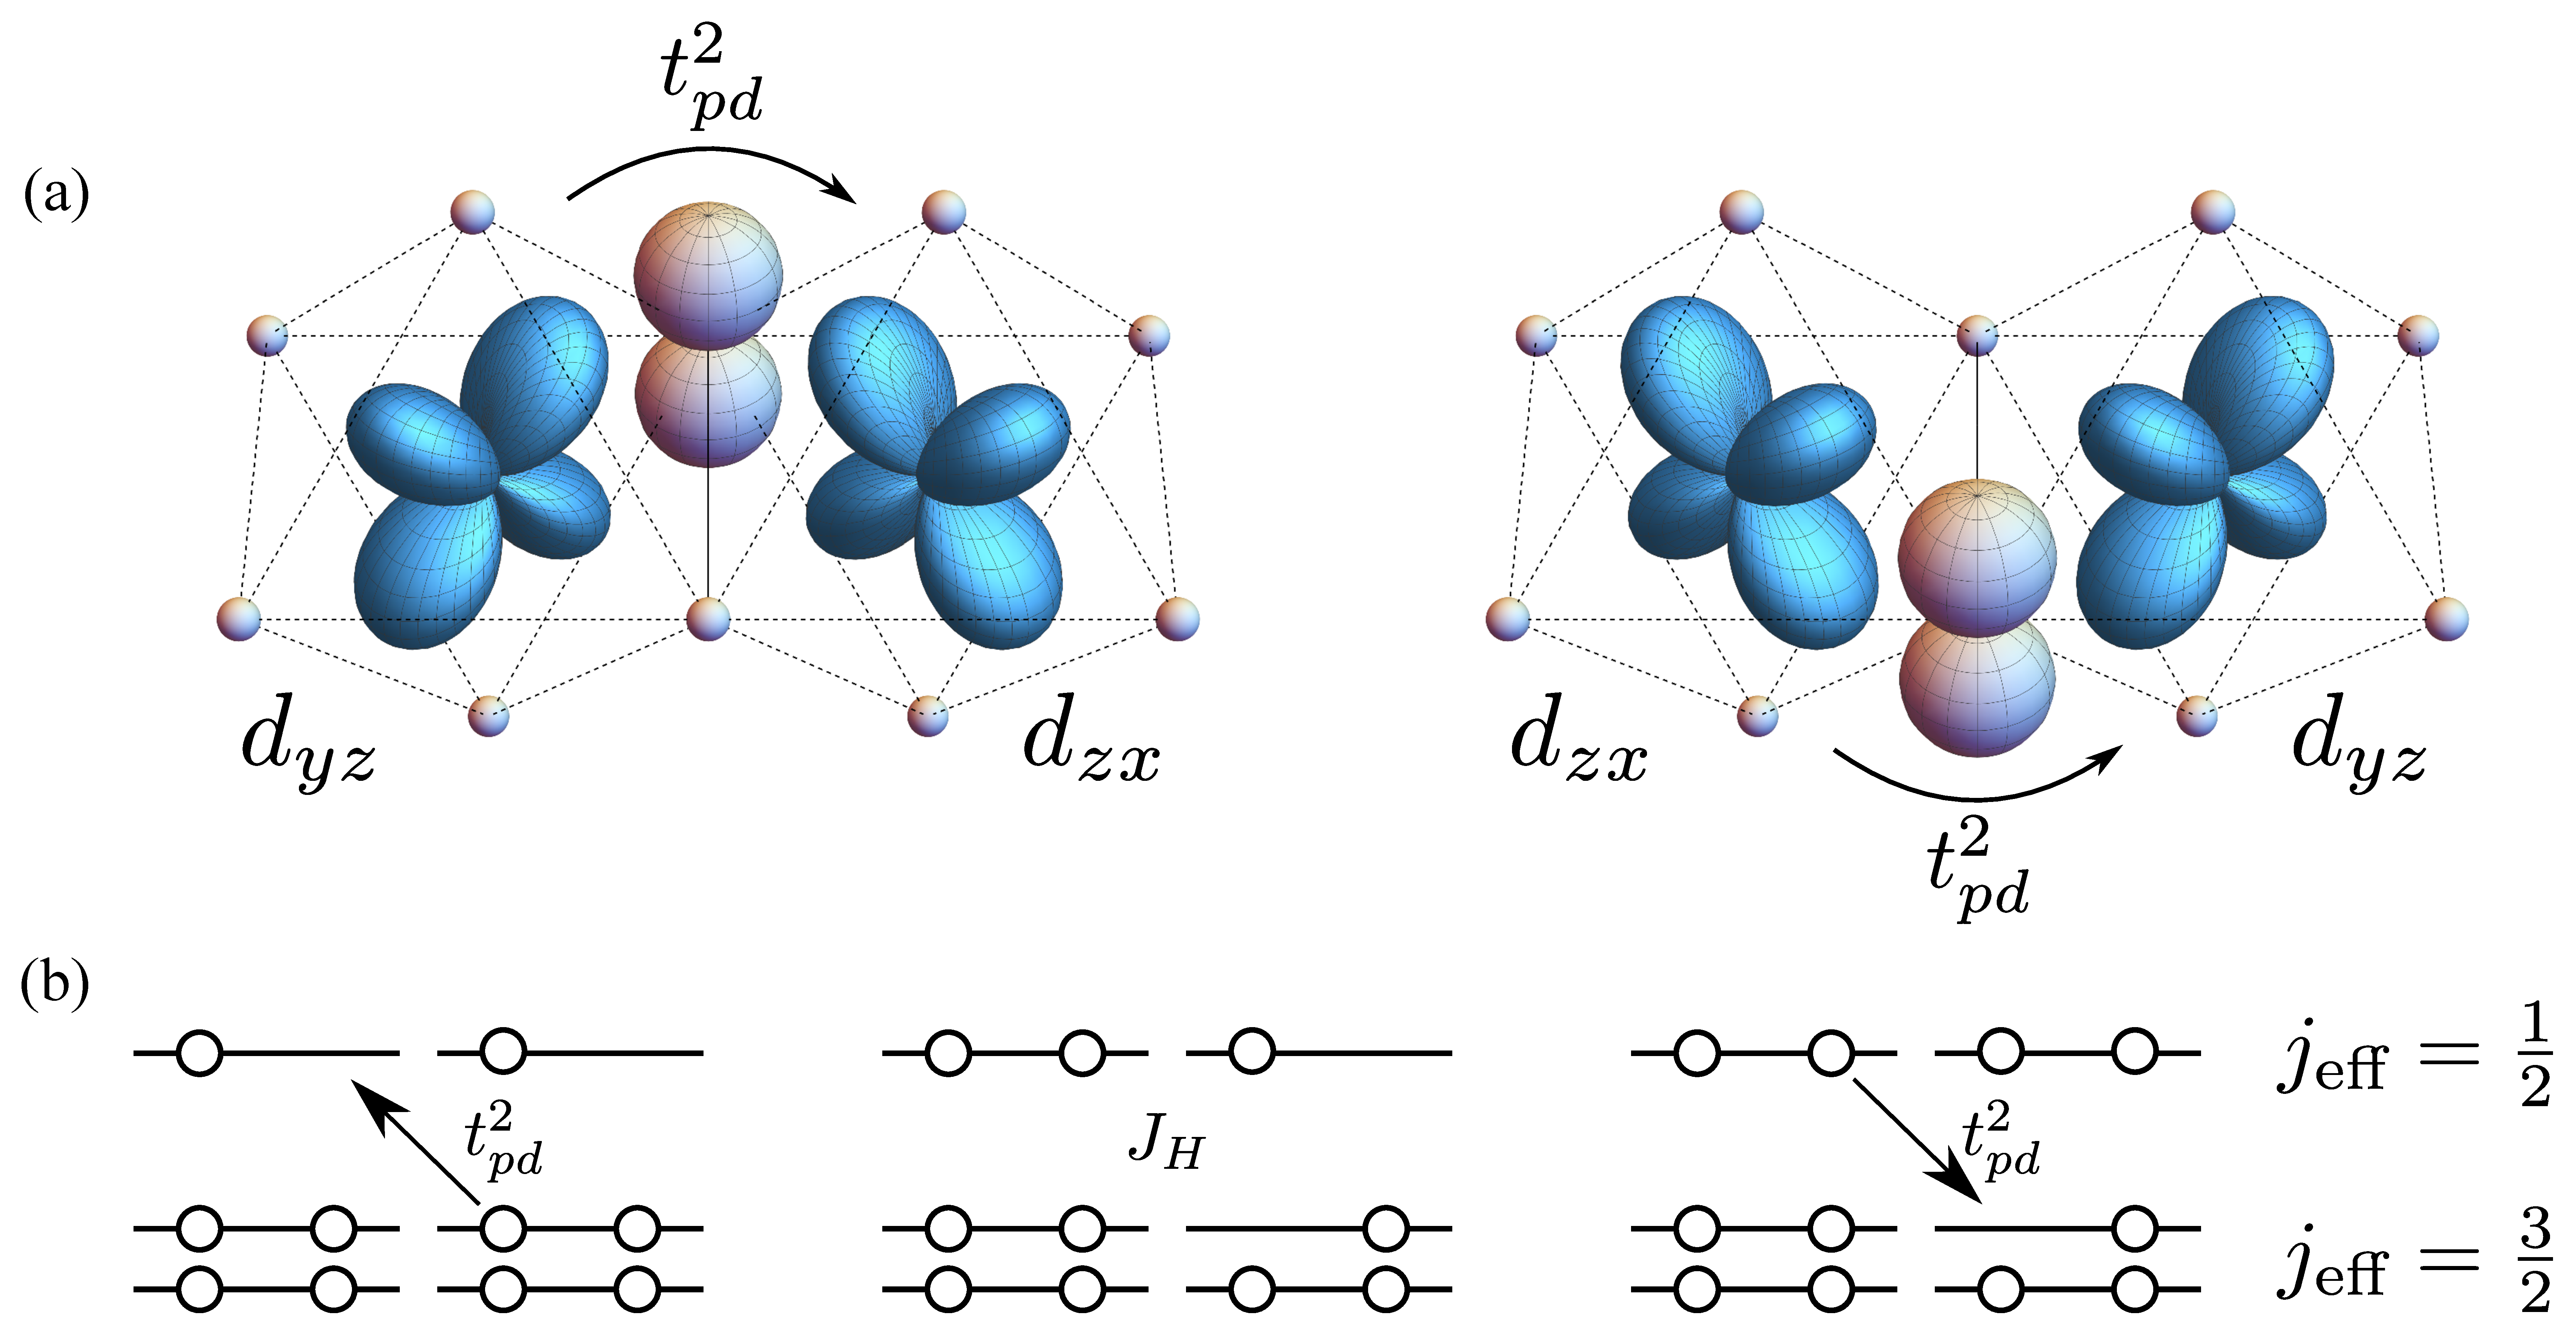
\includegraphics[width=\linewidth]{./chapter03/PerturbationTheory.pdf}
	\caption{
		(a) Two distinct 90$^{\circ}$ exchange paths for a hole to hop from the iridium site on the left to the iridium site on the right via an oxygen ligand.
		(b) Schematic of the exchange of a hole from the $j_{\rm eff} = 1/2$ state of the iridium ion on the left to a $j_{\rm eff} = 3/2$ state of the iridium ion on the right and back again.
	}
	\label{fig:chapter03_ExchangePaths}
\end{figure}
%
For the Mott insulating $5d$ iridates described above, a "spin" Hamiltonian may be derived via perturbation theory describing their interaction via the 90$^{\circ}$ exchange paths shown in Figure~\ref{fig:chapter03_ExchangePaths}~(a).
Here, the spin degrees of freedom correspond to the spin-orbit entangled $j_{\rm eff} = 1/2$ moments described above.
In this context, it will be simpler to think of there being a single hole at each iridium ion.
The superexchange mechanism originally considered by Jackeli and Khaliullin~\cite{JackeliPRL2009} allowed for hopping of holes between neighboring iridium ions via the oxygen ligands.
No direct $d-d$ hopping between iridium ions was considered, only hopping back and forth using the \textit{same} ligand was allowed, \ie, no cyclic exchange of holes around the Ir$_2$O$_2$ plaquette, and processes involving two holes on the same ligand were ignored due to strong Coulomb repulsion on the oxygen ions.
For the edge-sharing octahedra shown in Figure~\ref{fig:chapter03_ExchangePaths}~(a), a hole may hop from a $d_{zx}$-orbital to a $p_z$-orbital to a $d_{yz}$-orbital and back, or vice versa. 
In general, the active orbitals depend on the direction of the Ir-O-Ir exchange paths due to the anisotropic nature of the spin-orbit entangled moments.

For holes hopping between $j_{\rm eff} = 1/2$ orbitals it is clear that the resulting interaction is of the antiferromagnetic Heisenberg type $J \bS_i \cdot \bS_j$, where $J \sim t_{pd}^4 / U_d^2$, $t_{pd}$ is the hopping amplitude between $d$ and $p$ orbitals on the iridium and oxygen ions, respectively, $U_d$ is the local Coulomb repulsion on the iridium ions and $\bS_{i/j}$ are the effective spins living on neighboring iridium ions.
As can be seen in Figure~\ref{fig:chapter03_ExchangePaths}~(a), however, there are two such exchange paths -- one via the "upper" oxygen and one via the "lower" oxygen.
Jackeli and Khaliullin showed that the contributions from these two paths interfere destructively and cancel one another exactly.

There remains, however, the possibility for a hole to hop from the $j_{\rm eff} = 1/2$ doublet at one iridium site to the $j_{\rm eff} = 3/2$ quadruplet at the other site and then back (see Figure~\ref{fig:chapter03_ExchangePaths}~(b)).
In fact, the only relevant hopping is between $j_{\rm eff} = 1/2$ states and $m_{j_{\rm eff}} = \pm 3/2$ states~\cite{WinterJOP2017}.
Such processes ultimately generate a ferromagnetic interaction which does not affect the local arrangement of effective spins, \ie, it is of ferromagnetic Ising form $-J_K S_i^z S_j^z$, where $J_K \sim t_{pd}^4 J_H / U_d^2$ with the Hund's coupling $J_H$ acting between the $j_{\rm eff} = 1/2$ and excited $j_{\rm eff} = 3/2$ moments.
For other bond orientations with active $p_x$ or $p_y$ oxygen orbitals, the resulting anisotropic interaction instead couples the $x$- or $y$-components of the local moments, respectively.
For the honeycomb iridate compounds A$_2$IrO$_3$ to be discussed below, each iridium ion interacts with three neighbors through three distinct pairs of exchange paths (see Figure~\ref{fig:chapter03_HoneycombOctahedra}) and the resulting exchange produces exactly the Kitaev Hamiltonian,
%
\begin{equation}
	\op{H}_{\rm ex} = -J_K \sum_{\avg{i,j}_{\gamma}} S_i^{\gamma} S_j^{\gamma},
\end{equation}
%
where $\gamma$ is determined by the active $p$ orbital responsible for the superexchange between the neighboring $j_{\rm eff} = 1/2$ moments.
%
\begin{figure}[tb]
	\centering
	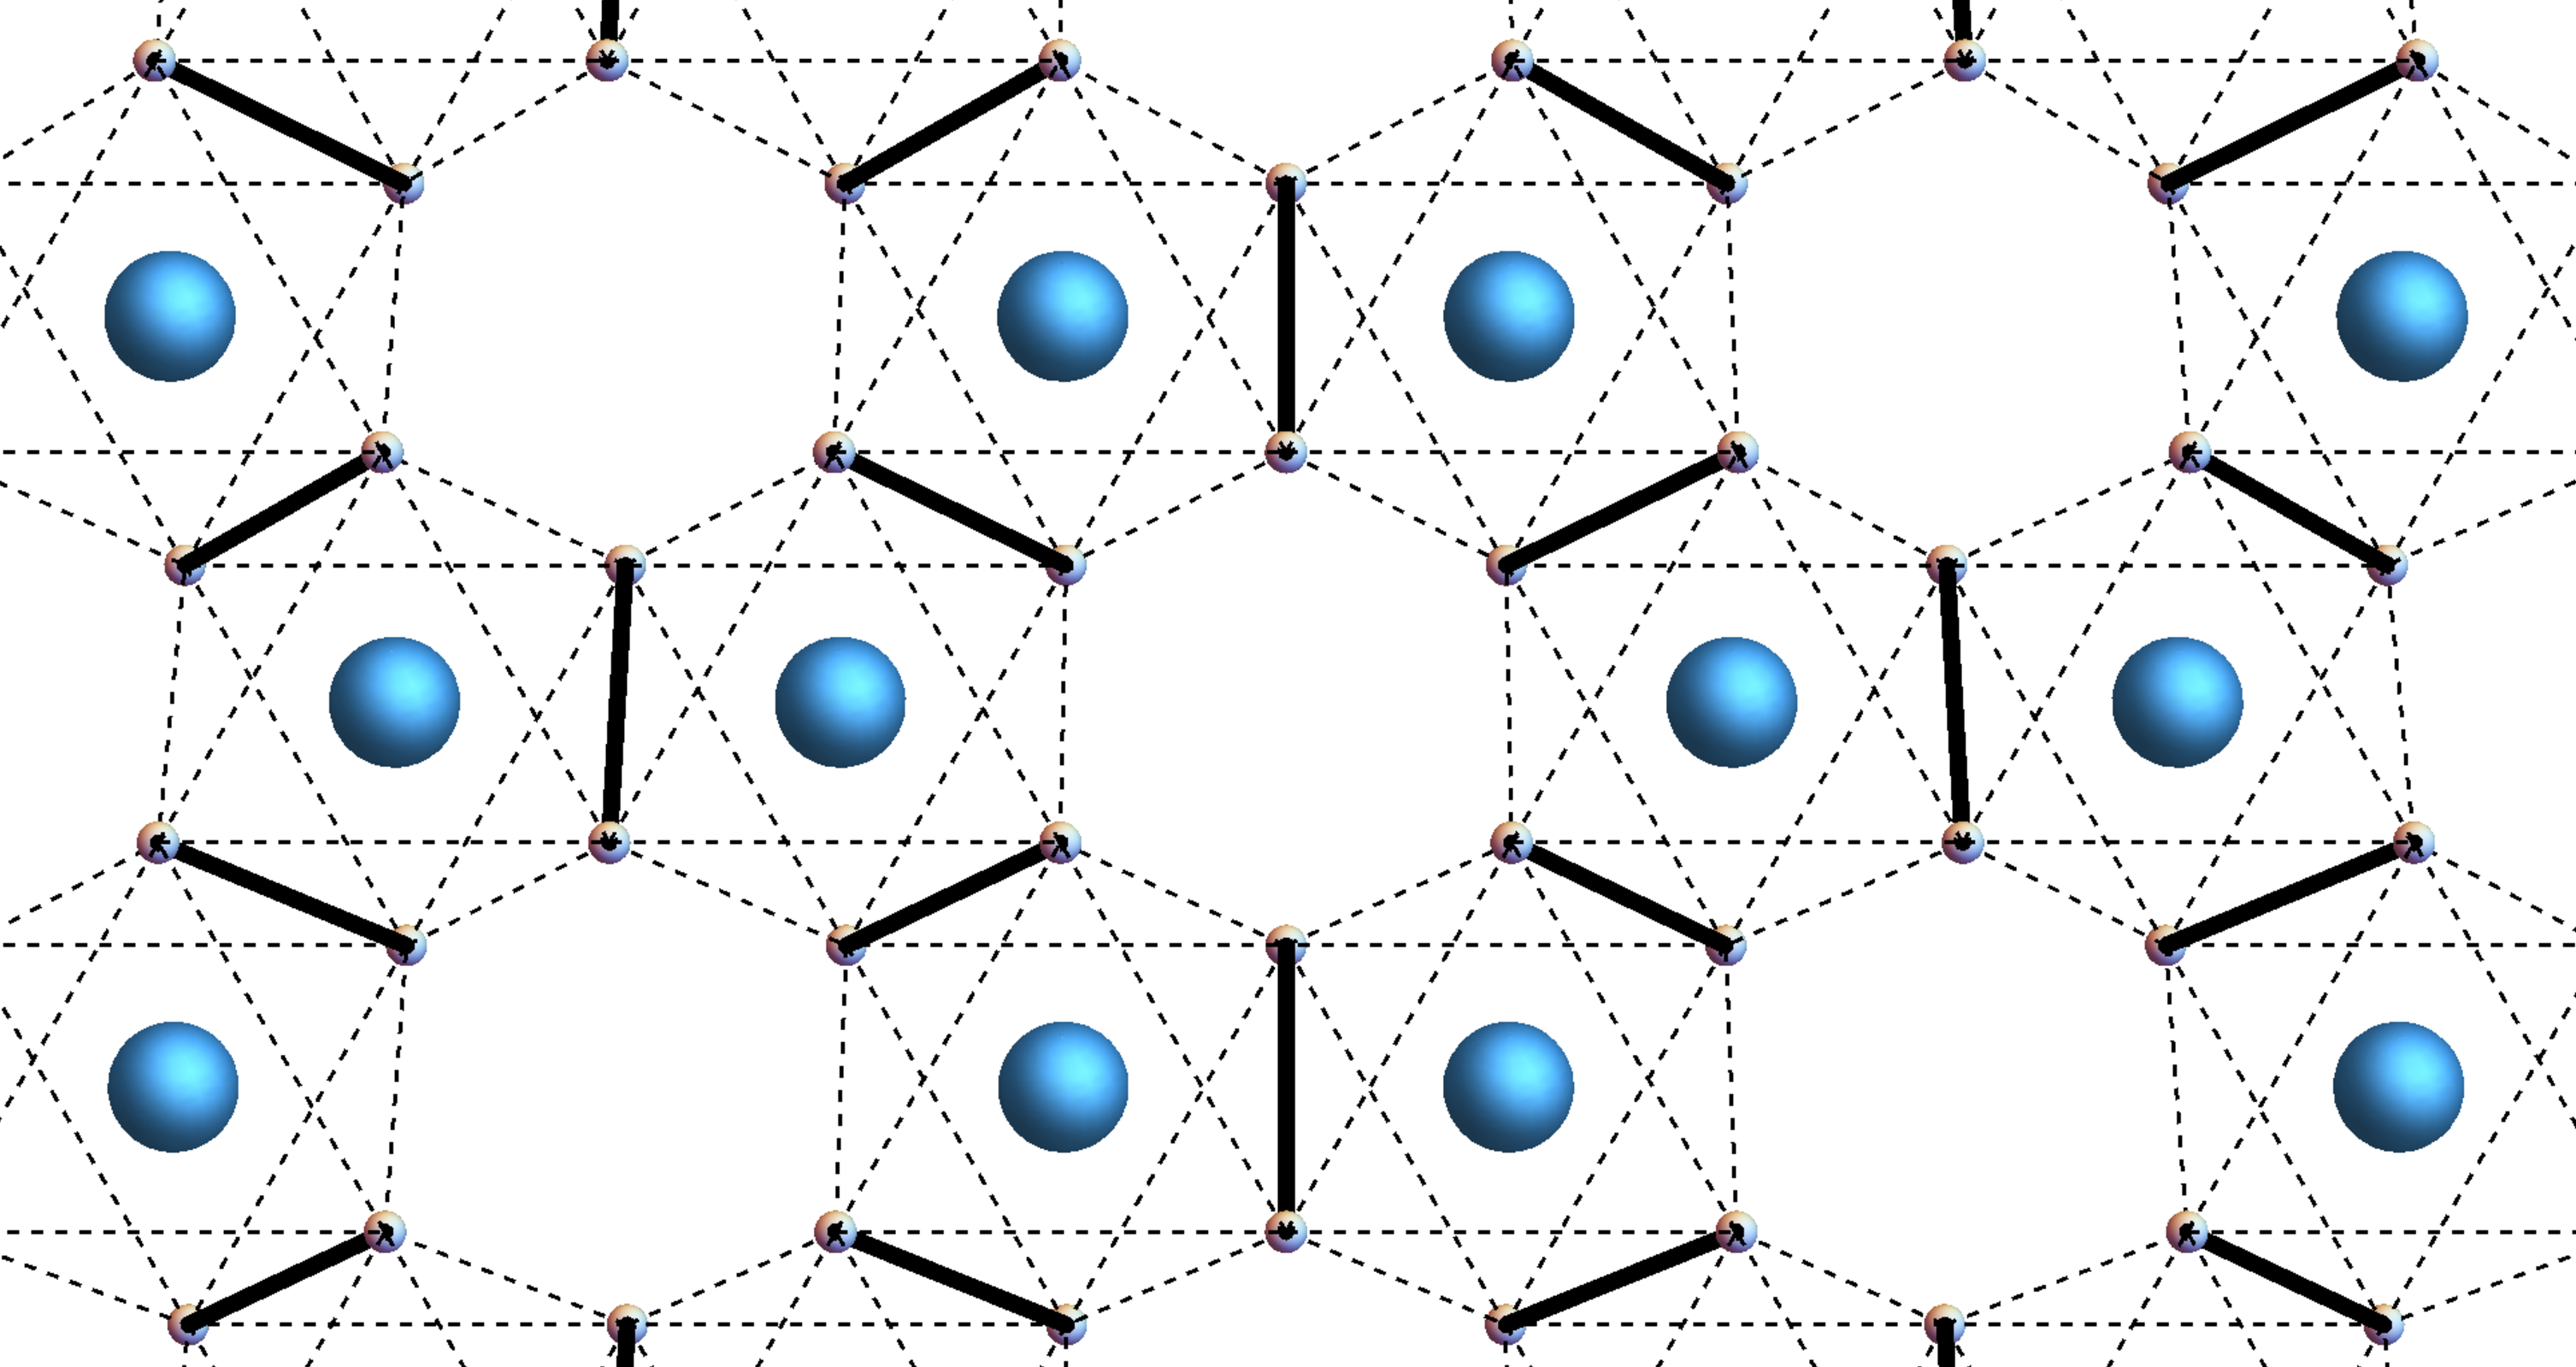
\includegraphics[width=0.8\linewidth]{./chapter03/HoneycombOctahedra.pdf}
	\caption{
		Honeycomb arrangement of iridium ions situated at the centers of edge-sharing oxygen octahedra.
		Shared edges responsible for Kitaev exchange between nearest neighbor iridium ions are marked with solid black lines.
	}
	\label{fig:chapter03_HoneycombOctahedra}
\end{figure}
%


%
%
\subsection{Additional exchange terms}
%
%
While the above mechanism for Kitaev exchange in a honeycomb iridate compound is elegant, in order to realistically discuss such a material a number of other effects should be considered.
To begin with, for compounds consisting of the heavier $4d$ and $5d$ transition metals, direct overlap of $d$ orbitals from neighboring ions may be significant.
As already mentioned, the analysis of the last section ignores the effects of direct $d-d$ hopping between neighboring iridium ions as well as cyclic exchange of holes around an Ir$_2$O$_2$ plaquette and the possibility of two holes simultaneously occupying an oxygen ion.
While the overlap of $d_{xy}$ orbitals from neighboring iridium ions leads to the usual antiferromagnetic Heisenberg exchange, the latter processes contribute both Heisenberg exchange as well as the anisotropic Kitaev interaction, yielding the effective model~\cite{ChaloupkaPRL2010}
%
\begin{equation}
	\op{H} = J \sum_{\avg{i,j}} \bS_i \cdot \bS_j - J_K \sum_{\avg{i,j}_{\gamma}} S^{\gamma}_i S^{\gamma}_j.
\end{equation}
%
In fact, allowing for exchange via \textit{all} $d$ orbitals introduces additional spin interactions leading to an effective Hamiltonian~\cite{WinterPRB2016,RauPRL2014}
%
\begin{align}
	\op{H} 	&= \sum_{\substack{\avg{i,j}_{\gamma}\\ \alpha,\beta \neq \gamma}} \Big(J_{ij} \bS_i \cdot \bS_j + K_{ij} S^{\gamma}_i S^{\gamma}_j + \Gamma_{ij} (S^{\alpha}_i S^{\beta}_j + S^{\beta}_i S^{\alpha}_j) \nonumber\\
			&\qquad\qquad+ \Gamma'_{ij} (S^{\gamma}_i S^{\alpha}_j + S^{\gamma}_i S^{\beta}_j + S^{\alpha}_i S^{\gamma}_j + S^{\beta}_i S^{\gamma}_j)\Big).
\end{align}
%

The $\Gamma'$ term above actually vanishes for cubic symmetry, however, real materials typically lack such perfect symmetry and tend to exhibit a trigonal distortion of the ligand octahedra~\cite{WinterJOP2017}.
Rather than producing local spin-orbit entangled $j_{\rm eff} = 1/2$ moments, such a distorted crystal field splits the degeneracy of the $t_{2g}$ orbitals and results in local moments with a different mixture of spin and orbital character.
For significantly small distortions which only partially quench the orbital angular momentum, additional anisotropic exchange terms are present, \eg, the $\Gamma'$ term above.
However, for distortions which completely lift the $t_{2g}$ degeneracy the local moments are pure $s = 1/2$ moments and exhibit nearly isotropic Heisenberg exchange~\cite{WinterJOP2017}.
Additionally, a finite Dzyaloshinskii-Moriya interaction $\bm{D}\cdot(\bS_i \times \bS_j)$ is permitted for \textit{second}-nearest neighbors in all Kitaev candidate lattices as well as certain nearest-neighbor bonds in the 3D materials~\cite{WinterPRB2016}.


%
%
%%%%%%%%%%%%%%%%%%%%%%%%%%%%%%%%%%%%%%%%%%%%%%%%%%%%%%%%%%%%%%%%%%%%%%%%%%%%%%%%%%%%%%%%
\section{Kitaev materials}
\label{section:chapter03_Materials}
%%%%%%%%%%%%%%%%%%%%%%%%%%%%%%%%%%%%%%%%%%%%%%%%%%%%%%%%%%%%%%%%%%%%%%%%%%%%%%%%%%%%%%%%
%
%
This section provides a brief overview of the two-dimensional honeycomb materials, namely the iridates Na$_2$IrO$_3$ and $\alpha$-Li$_2$IrO$_3$ and the honeycomb ruthenate RuCl$_3$, as well as the three-dimensional hyperhoneycomb and stripy-honeycomb iridates $\beta$-Li$_2$IrO$_3$ and $\gamma$-Li$_2$IrO$_3$, respectively.


%
%
%%%%%%%%%%%%%%%%%%%%%%%%%%%%%%%%%%%%%%%%%%%%%%%%%%%%%%%%%%%%%%%%%%%%%%%%%%%%%%%%%%%%%%%%
\subsubsection{Honeycomb Na$_2$IrO$_3$}
%%%%%%%%%%%%%%%%%%%%%%%%%%%%%%%%%%%%%%%%%%%%%%%%%%%%%%%%%%%%%%%%%%%%%%%%%%%%%%%%%%%%%%%%
%
%
The first Kitaev material extensively studied at low temperatures was the honeycomb iridate Na$_2$IrO$_3$~\cite{SinghPRB2010}.
This material, as well as its counterpart $\alpha$-Li$_2$IrO$_3$ discussed below, is composed of weakly coupled honeycomb planes of oxygen octahedra with iridium ions at their centers.
The compound has been identified as a Mott insulator via electrical resistivity~\cite{SinghPRB2010} and ARPES measurements which indicate nearly dispersionless $t_{2g}$ bands~\cite{CominPRL2012,AlidoustPRB2016,LuepkePRB2015}.
Measurements of the crystal field splitting using resonant inelastic x-ray scattering confirm a spin-orbit entangled $j_{\rm eff} = 1/2$ picture~\cite{GretarssonPRL2013}.

The  material was found to exhibit magnetic order below a N\'eel temperature of $T_N = 13 - 18$ K, where it has been observed to develop a zigzag order~\cite{SinghPRB2010,ChoiPRL2012,YePRB2012,LiuPRB2011}.
Although direct evidence of a dominant Kitaev exchange has been provided by diffuse resonant x-ray scattering~\cite{BarreiroNatPhys2015}, other exchange terms have been estimated to be between 10-30\% of the nearest-neighbor Kitaev exchange~\cite{KatukuriNJP2014,WinterPRB2016,KimchiPRB2011,ChoiPRL2012,ChaloupkaPRB2016}.
Despite Kitaev interactions dominating in agreement with the picture set forth by Jackeli and Khaliullin, additional exchange interactions work to stabilize the zigzag order at low temperatures.


%
%
%%%%%%%%%%%%%%%%%%%%%%%%%%%%%%%%%%%%%%%%%%%%%%%%%%%%%%%%%%%%%%%%%%%%%%%%%%%%%%%%%%%%%%%%
\subsubsection{Honeycomb $\alpha$-Li$_2$IrO$_3$}
%%%%%%%%%%%%%%%%%%%%%%%%%%%%%%%%%%%%%%%%%%%%%%%%%%%%%%%%%%%%%%%%%%%%%%%%%%%%%%%%%%%%%%%%
%
%
Like its counterpart above, $\alpha$-Li$_2$IrO$_3$ has been established as a Mott insulating honeycomb material with dominant Kitaev exchange interactions~\cite{KobayashiJMC2003,SinghPRL2012}.
Evidence of spin-orbit entangled $j_{\rm eff} = 1/2$ moments has been obtained through measurements of crystal field splitting using resonant inelastic x-ray scattering~\cite{GretarssonPRL2013}.
$\alpha$-Li$_2$IrO$_3$ also develops long-range magnetic order below a  N\'eel temperature of $T_N = 15$ K, where it hosts incommensurate counter-rotating spirals~\cite{SinghPRL2012,WilliamsPRB2016}.
The formation of this incommensurate state also requires a large Kitaev exchange~\cite{WilliamsPRB2016}, however, the role of other exchange interactions in this material remains unclear~\cite{WinterJOP2017}.


%
%
%%%%%%%%%%%%%%%%%%%%%%%%%%%%%%%%%%%%%%%%%%%%%%%%%%%%%%%%%%%%%%%%%%%%%%%%%%%%%%%%%%%%%%%%
\subsubsection{Honeycomb $\alpha$-RuCl$_3$}
%%%%%%%%%%%%%%%%%%%%%%%%%%%%%%%%%%%%%%%%%%%%%%%%%%%%%%%%%%%%%%%%%%%%%%%%%%%%%%%%%%%%%%%%
%
%
More recently, much interest has been expressed in the $4d$ compound $\alpha$-RuCl$_3$ as a possible \textit{proximate} Kitaev spin liquid material.
The chlorine octahedra exhibit a nearly perfect cubic symmetry with minimal trigonal distortion and the ruthenium ions form a nearly perfect honeycomb lattice~\cite{TrebstARXIV2017}.
The material has been identified as a Mott insulator via resistivity and photoconductivity measurements~\cite{BinottoPSS1971} as well as photoemission~\cite{ZhouPRB2016,KoitzschPRL2016,SinnSciRep2016} and inverse photoemission experiments~\cite{SinnSciRep2016}.
Spin-orbit coupling plays less of a role than in the iridates due to the lighter $4d$ ruthenium ions~\cite{JohnsonPRB2015}, however, indications of $j_{\rm eff} = 1/2$ moments have been given by x-ray absorption spectroscopy~\cite{PlumbPRB2014,LampenPRL2017}, electron energy loss spectroscopy~\cite{KoitzschPRL2016} and low-energy optical response~\cite{SandilandsPRB2016}.

High quality single crystals of $\alpha$-RuCl$_3$ have been observed to exhibit a transition at $T_N = 7$ K~\cite{BanerjeeScience2017} to a zigzag ordered phase~\cite{JohnsonPRB2015,SearsPRB2015,BanerjeeNatMat2016}.
Raman scattering measurements have revealed a continuum of magnetic excitations well above the ordering temperature~\cite{SandilandsPRL2015} reminiscent of predictions for a pure Kitaev spin liquid phase~\cite{KnollePRL2014}.
This excitation continuum is further supported by inelastic neutron scattering experiments~\cite{BanerjeeScience2017,RanPRL2017}.
It has been suggested~\cite{NasuNatPhys2016} that the temperature dependence of the continuum implies the existence of fractionalized fermionic excitations and claims that $\alpha$-RuCl$_3$ is in close proximity to a Kitaev spin liquid phase.
However, it has been pointed out that these observations may also be explained by off-diagonal exchange resulting in the decay of magnons into a broad continuum of multi-magnon states~\cite{WinterNatComm2017}.
This conclusion is independent of proximity to a Kitaev spin liquid state and demonstrates that such proximity is not necessarily implied by the data.


%
%
%%%%%%%%%%%%%%%%%%%%%%%%%%%%%%%%%%%%%%%%%%%%%%%%%%%%%%%%%%%%%%%%%%%%%%%%%%%%%%%%%%%%%%%%
\subsubsection{Hyperhoneycomb $\beta$-Li$_2$IrO$_3$ and stripy-honeycomb $\gamma$-Li$_2$IrO$_3$}
%%%%%%%%%%%%%%%%%%%%%%%%%%%%%%%%%%%%%%%%%%%%%%%%%%%%%%%%%%%%%%%%%%%%%%%%%%%%%%%%%%%%%%%%
%
%
The discovery of the three-dimensional Li$_2$IrO$_3$ polymorphs on the tricoordinated honeycomb and stripy-honeycomb lattices in the form of $\beta$-Li$_2$IrO$_3$~\cite{TakayamaPRL2015} and $\gamma$-Li$_2$IrO$_3$~\cite{ModicNatComm2014}, respectively, drove much of the theoretical interest in three-dimensional Kitaev spin liquids -- including the work reported in this thesis.
Both materials have been shown to be Mott insulators via DC resistivity measurements~\cite{ModicNatComm2014,TakayamaPRL2015}.
\textit{Ab initio} estimates suggest crystal field splitting in the $\beta$ phase to be on par with the honeycomb $\alpha$ phase~\cite{KatukuriSP2016,KimEPL2015}, whereas estimates for trigonal field terms in the $\gamma$ phase are much larger~\cite{WinterJOP2017}.

Both the $\beta$ and $\gamma$ phases exhibit magnetically ordered incommensurate counter-rotating spiral phases below $T_N = 37$ K~\cite{BiffinPRB2014,TakayamaPRL2015} and $T_N = 39.5$ K~\cite{ModicNatComm2014,BiffinPRL2014}, respectively.
Just as in the $\alpha$ phase, the magnetic order of the $\beta$ and $\gamma$ phases leaves a lot of room for interpretation of the exchange interactions.
Both phases can be reproduced with a Heisenberg-Kitaev model with an additional Ising anisotropy~\cite{KimchiPRB2014,KimchiPRB2015}.
However, they have also been shown to be consistent with a nearest-neighbor $J-K-\Gamma$ model~\cite{KimEPL2015,LeePRB2015}.
\textit{Ab initio} studies of the $\beta$ phase further support the $J-K-\Gamma$ picture~\cite{KatukuriSP2016,KimPRB2016,KimEPL2015}, however, it has also been suggested that longer-range interactions play an important role in these materials~\cite{KatukuriSP2016}.


%
%
%%%%%%%%%%%%%%%%%%%%%%%%%%%%%%%%%%%%%%%%%%%%%%%%%%%%%%%%%%%%%%%%%%%%%%%%%%%%%%%%%%%%%%%%
\section{Summary}
\label{section:chapter03_Summary}
%%%%%%%%%%%%%%%%%%%%%%%%%%%%%%%%%%%%%%%%%%%%%%%%%%%%%%%%%%%%%%%%%%%%%%%%%%%%%%%%%%%%%%%%
%
%
This chapter focused on the solid state realization of Kitaev's honeycomb model in certain spin-orbit assisted Mott insulating transition metal oxides.
It was shown how the interplay of strong crystal field effects and strong spin-orbit coupling in such materials results in the splitting of spin and orbital degeneracies to yield a $j_{\rm eff} = 1/2$ degree of freedom.
Due to the narrow bandwidth of the $j_{\rm eff} = 1/2$ doublet, even a relatively weak on-site Coulomb repulsion results in a local moment picture.
The mechanism of ligand-assisted superexchange was discussed which Jackeli and Khaliullin put forth to predict Kitaev interactions in these materials.
Additional magnetic exchange terms were also discussed, the inclusion of which are necessary for a realistic description of the Kitaev materials.
A brief discussion of the relevant two- and three-dimensional materials revealed that these other exchange mechanisms lead to long-range magnetic order in all of the Kitaev materials discovered so far.

It should be mentioned that there have been other proposals for engineering solid state incarnations of Kitaev physics.
In 2017, the Oshikawa group proposed designing Kitaev materials in metal-organic-frameworks (MOF)~\cite{MasahikoPRL2017}.
In an MOF, rather than the edges of ligand octahedra being shared \textit{directly}, additional organic ligands such as $({\rm C}_2{\rm O}_4)^{2-}$ connect the edges of neighboring octahedra.
The idea is that the electron density of the organic ligands screens the wave functions of the metal ions, thereby reducing the direct $d-d$ hopping that leads to most of the other \textit{non}-Kitaev exchange interactions.
Very recently, it has been proposed that Kitaev physics may also be observed in the rare earth magnets with $4f$ rather than $4d/5d$ electrons~\cite{LiPRB2017,LuoARXIV2019}.	% Transition Metal Oxides as Kitaev Materials
%%%%%%%%%%%%%%%%%%%%%%%%%%%%%%%%%%%%%%%%%%%%%%%%%%%%%%%%%%%%%%%%%%%%%%%%%%%%%%%%%%%%%%%%
\chapter[Quantum Order and Projective Symmetry Groups]{Quantum Order and\linebreak Projective Symmetry Groups}
\label{chapter:ProjectiveSymmetryGroup}
%%%%%%%%%%%%%%%%%%%%%%%%%%%%%%%%%%%%%%%%%%%%%%%%%%%%%%%%%%%%%%%%%%%%%%%%%%%%%%%%%%%%%%%%
%
%
On the topic of approaching new problems in physics, P.~W. Anderson wrote in his 1984 textbook \textit{Basic notions of condensed matter physics}~\cite{Anderson1984},
%
\begin{quote}
	"the two most important principles of condensed matter physics~\ldots~are, first, broken symmetry, which tells us what the order parameter is and what symmetry it breaks are the most vital questions; and, second, the continuity principle, which tells us to search for the right simple problem when confronted with a complicated one."
\end{quote}
%
In the former case, he is referring to Landau's theory of phase transitions~\cite{LandauNature1936,LandauZETF1937,GinzburgZETF1950}.
In regards to the latter, he goes on to use Landau's Fermi liquid theory~\cite{LandauZETF1956,LandauZETF1957,LandauZETF1958} to illustrate the power of the principle of adiabatic continuity.

Landau's theory of phase transitions makes the observation that, given a Hamiltonian $\op{H}$ along with a symmetry group $G$ which preserves it, although the Hamiltonian may possess a given symmetry, the dynamics of the system singles out a ground state which breaks that symmetry.
This process goes by the name of \textit{spontaneous symmetry breaking}.
According to Landau's theory, different phases of matter can be distinguished by their symmetries.
Thus, a given Hamiltonian in different parameter or temperature regimes may give rise to different phases of matter by virtue of the mechanism of spontaneous symmetry breaking.

Landau's theory, furthermore, allows for the definition of a local order parameter which signals the spontaneous breaking of a symmetry and, thus, the onset of order in the system.
A ground state of the system is seen not to be invariant under $G$ if there exists an order parameter $\op{O}$ and one $g \in G$ such that $g \op{O} \neq \op{O}$ and $\psi_{\op{O}} \equiv \avg{\op{O}} \neq 0$.
Any specific ground state is characterized by a maximal subgroup $H$ which still preserves it, \ie,
%
\begin{align}
	\psi_{h \op{O}} &= \psi_{\op{O}} \qquad \forall h \in H \nonumber\\
	\psi_{g \op{O}} &\neq \psi_{\op{O}} \qquad \forall g \in G/H.
\end{align}
%
Having identified the order parameter, one may write down an effective free energy functional for the system in terms of $\psi_{\op{O}}$ in the vicinity of the phase transition, yielding a mean-field description of the transition from the disordered phase to the ordered phase. 
The combination of Landau's theory with the ideas of Wilson's renormalization group~\cite{WilsonPRB1971I,WilsonPRB1971II,WilsonPRL1972,WilsonRMP1975} allowed for the definition of \textit{universality classes}, unifying phase transitions in seemingly disparate physical systems into equivalence classes defined by their universal critical behavior.
Additionally, Nambu and Goldstone~\cite{NambuPRL1960,GoldstoneINC1961} showed that a generic spontaneously broken continuous symmetry implies the existence of massless scalar bosons corresponding to long-wavelength excitations of the order parameter.
This synthesis of ideas has been wildly successful and it was long thought to provide a complete understanding of the different phases of matter.

Landau's Fermi liquid theory has been similarly fruitful, providing a\linebreak phenomenological description of many strongly interacting fermion systems such as (normal) liquid $^3$He and normal metals~\cite{SilinJETP1958,SilinJETP1959} in terms of \textit{nearly free}\linebreak \textit{fermions}~\cite{Leggett2006}.
Landau argued that, in the absence of an electronic phase transition, the ground state of the non-interacting Fermi gas would be adiabatically transformed into the ground state of the interacting system as the interaction strength was slowly increased.
Furthermore, he assumed that each excited state of the ideal Fermi gas is likewise adiabatically transformed into a corresponding excited state of the interacting Fermi liquid, \ie, there is a one-to-one correspondence between the particle and hole excitations of the Fermi gas and the so-called \textit{quasiparticle} and \textit{quasihole} excitations of the Fermi liquid which carry the same spin, charge and momentum as the excitations in the non-interacting system, but with a different \textit{effective mass}.\footnote{For simplicity, a momentum- and spin-conserving potential is assumed.}

A consistent application of Fermi liquid theory must also include interactions between quasiparticles (quasiholes) at lowest order and, thus, scattering between quasiparticles, leading to a finite quasiparticle lifetime.
Such a finite lifetime would seem to spoil the above arguments which depend on the adiabatic evolution of free fermions into quasiparticles, however, for excitations sufficiently close to the Fermi surface (as one would expect for low temperatures), the quasiparticle lifetimes become sufficiently long to justify the established one-to-one correspondence between quasiparticle excitations of the Fermi liquid and excitations of the Fermi gas.
This \textit{nearly free} quasiparticle picture results in certain equilibrium properties of the Fermi liquid such as specific heat, static compressibility, spin- and charge-susceptibilities being qualitatively unchanged from those of the ideal Fermi gas at low temperatures, with prefactors simply being renormalized by replacing the bare mass with the effective mass and/or by effects of quasiparticle scattering~\cite{Pines1966,Coleman2015}.
Besides just possessing renormalized properties of a Fermi gas, the Fermi liquid also has entirely new characteristics such as \textit{zero sound} -- supersonic density oscillations in the Fermi liquid resulting from interactions between the quasiparticles~\cite{KeenPL1963,AbelPRL1966,MerminPR1967}.

Landau already understood that the Fermi liquid theory is always potentially unstable to superconductivity as it implies the presence of a phase transition.
By the late 1960's it became clear that a Fermi liquid is generically unstable in one-dimension, giving rise instead to a separation of spin and charge degrees of freedom in what is now known as a Luttinger liquid~\cite{LuttingerJMP1963,HaldaneJoPC1981}.
Eventually, the Fermi liquid theory was given a more rigorous footing in terms of the renormalization group theory, (re)establishing its inapplicability in one-dimension, as well its instability to superconductivity, or to the formation of charge- or spin-density wave orders for nested Fermi surfaces in two- and three-dimensions~\cite{BenfattoPRB1990,ShankarRMP1994}.
However, the renormalization group approach also showed that the Fermi liquid is not \textit{generically} unstable in two- and three-dimensions as it is in 1D, implying a wide range of applicability.

The overwhelming effectiveness of these two theories in describing the physics of many-body systems lead to a feeling that there were no new important concepts to find and that the only thing left to do was apply Landau's theories to different kinds of systems~\cite{Wen2004}.
However, the discovery of the fractional quantum Hall effect by Tsui, St\"ormer and Gossard~\cite{TsuiPRL1982} and its phenomenological description by Laughlin~\cite{LaughlinPRL1983} as a new type of quantum liquid lead to the realization that Landau's theories could not be used to describe \textit{all} states of matter~\cite{WenPRB1989,WenPRB1990}.
Different fractional quantum Hall (FQH) states possess the same symmetry and, thus, cannot be characterized by the paradigm of symmetry breaking.

The concept of \textit{topological order} was introduced~\cite{WenJMPB1990,WenAiP1995} to characterize these states for which no physical, local order parameter could be defined and which host fractionalized collective excitations possessing quantum numbers distinct from those of the electrons from which they are formed.
The theory of topological order proposed to characterize different FQH states by the differing topology of their respective wave functions.
Such a classification is successful for a class of FQH states called Abelian FQH states, \ie, those states for which the low-energy excitations obey Abelian statistics~\cite{BlokPRB1990a,BlokPRB1990b,ReadPRL1990,FroehlichNPB1991,FroehlichRMP1993}.
The non-trivial topology of the FQH wave functions leads to a robust topological ground state degeneracy which depends only on the genus of the surface on which the theory is defined~\cite{HaldanePRL1983,HaldanePRB1985,WenPRB1990}.
Furthermore, the non-trivial topology of the bulk wave function implies the existence of gapless excitations on the surface of the FQH liquid~\cite{WenIJMP1992}.

While topological order can be used to describe a large class of \textit{gapped} quantum liquids such as the Abelian FQH states, the broader designation of \textit{quantum order} can be applied to a broader class of systems (including \textit{gapless} quantum liquids), of which the topologically ordered systems form a subclass.
Quantum order aims to describe the universality classes of quantum ground states as opposed to the universality classes of classical statistical states described by Landau's theory~\cite{WenPRB2002,WenPLA2002}.
There is currently no complete theory to describe all possible quantum orders, however, a large class of quantum orders can be described by an object called a \textit{projective symmetry group} (PSG).
Whereas Landau's theory distinguished classical phases by their symmetries and determined the structure of low-energy excitations without needing to know the details of a system~\cite{NambuPRL1960,GoldstoneINC1961}, the PSG allows for the classification of different \textit{quantum} phases which have the same symmetry, while similarly determining the structure of low-energy excitations without the need to know the details of a system.
In remarkable contrast to symmetry-breaking orders which generate and protect gapless, scalar Nambu-Goldstone bosons, quantum orders can generate and protect gapless gauge bosons and gapless fermions, even in pure local bosonic models~\cite{Wen2004}.

The remainder of this chapter is structured as follows.
The basic ideas behind the PSG are introduced in Section~\ref{section:chapter04_OverviewOfTheProjectiveSymmetryGroup} as well as the ideas behind its use in classifying quantum ground states in the context of quantum spin liquids.
These concepts are developed in greater detail in Sections~\ref{section:chapter04_ProjectiveConstructionOfQuantumSpinLiquids}--\ref{section:chapter04_TheProjectiveSymmetryGroup}.
In Section~\ref{section:chapter04_ApplicationToTheKitaevHoneycombModel}, these concepts are applied to the Kitaev honeycomb model discussed in Chapter~\ref{chapter:KitaevHoneycombModel}.
Finally, Section~\ref{section:chapter04_Summary} provides a brief summary.


%
%%%%%%%%%%%%%%%%%%%%%%%%%%%%%%%%%%%%%%%%%%%%%%%%%%%%%%%%%%%%%%%%%%%%%%%%%%%%%%%%%%%%%%%%
\section{Overview of the projective symmetry group}
\label{section:chapter04_OverviewOfTheProjectiveSymmetryGroup}
%%%%%%%%%%%%%%%%%%%%%%%%%%%%%%%%%%%%%%%%%%%%%%%%%%%%%%%%%%%%%%%%%%%%%%%%%%%%%%%%%%%%%%%%
%
This section introduces the basic ideas behind the construction of mean-field spin liquids using the projective symmetry group.
The idea is to provide an overview of concepts that will be made more precise in the following sections.

The starting point is a Hamiltonian of quantum spin-1/2 moments on a lattice, \eg,
%
\begin{equation}
	\op{H}_{\rm spin} = \sum_{i,j} J_{ij}~\bsigma_i \cdot \bsigma_j,
\end{equation}
%
where $\bsigma$ is a vector of Pauli matrices.
In a classically ordered phase, a standard mean-field decoupling of the quantum spins may be performed, resulting in a mean-field Hamiltonian, \eg,
%
\begin{equation}
	\op{H}_{\rm mean} = \sum_{\avg{i,j}} J_{ij} (\avg{\bsigma_i} \cdot \bsigma_j + \bsigma_i \cdot \avg{\bsigma_j} - \avg{\bsigma_i} \cdot \avg{\bsigma_j}),
\end{equation}
%
in order to determine the nature of the classical mean-field ground state.
Moreover, the low energy excitations of the system may be studied by including the fluctuations above the mean-field.
However, in a quantum spin liquid ground state, the spins do not order even at zero temperature and, thus, the above spin mean-field decoupling fails due to the vanishing expectation value $\avg{\bsigma_i} = 0$, or, more generally, due to the absence of \textit{any} local order parameter.

A possible solution to this problem came in the form of the slave-particle approach~\cite{BaskaranSSC1987}, whereby the spin degrees of freedom are replaced by fermionic partons via the transformation
%
\begin{equation}
	\bsigma_i = f\dag_{i\alpha} \btau_{\alpha\beta} f_{i\beta},
\end{equation}
%
where $\btau$ is the vector of Pauli matrices acting on the spin indices $\alpha,\beta$ of the fermion operators.
This representation comes with the cost of an enlarged Hilbert space due to the inclusion of the unphysical empty and doubly-occupied fermion states.
The advantage, however, is that a mean-field decoupling of the \textit{fermions} rather than of the spins could be performed, with the additional half-filling constraint
%
\begin{equation}
	f\dag_{i\alpha} f_{i\alpha} = 1
\end{equation}
%
being enforced either by Lagrange multiplier or by a Gutzwiller projection of the mean-field state to the physical subspace.

It was later seen~\cite{AffleckPRB1988,DagottoPRB1988} that the parton approach actually contained a hidden local $SU(2)$ gauge redundancy and that the mean-field Hamiltonian could be framed as a quadratic theory of fermions coupled to an $SU(2)$ gauge field.
In this framework, the inclusion of Lagrange multipliers to enforce the half-filling constraint could be interpreted as the temporal component of the $SU(2)$ gauge field.
Now a fermionic mean-field ground state could be found wherein the gauge field is chosen to be static and the restriction of the fermions to the physical, half-filled subspace could be performed by including temporal fluctuations of the gauge field.

It was realized by Wen~\cite{WenPRB2002} that physical symmetry operations on the spins may need to be paired with a gauge transformation in order to preserve a given mean-field configuration and that the exact nature of how symmetries acted in the gauge sector could be an important way of classifying \textit{different} mean-field spin liquids with the \textit{same} symmetries.
The universality classes deriving from this line of thought go by the name \textit{projective symmetry groups}.
A projective symmetry group $PSG$ of a quantum spin liquid phase with symmetry group $SG$ is defined as
%
\begin{equation}
	SG = PSG/IGG,
\end{equation}
%
where $IGG$ is the set of pure gauge transformations leaving the mean-field \textit{Ansatz} unchanged and is known as the \textit{invariant gauge group} (IGG).
In words, the projective symmetry group is the group of combined symmetry and gauge transformations which leave a given mean-field \textit{Ansatz} unchanged up to unitary gauge equivalence.

This idea allowed for the possibility of classifying mean-field spin liquids which possess all of the same symmetries, but which differ in their projective representations.
Additionally, at low energy, fluctuations of the gauge field away from the mean-field \textit{Ansatz} must respect the invariant gauge group, making the IGG an additional way of coarsely classifying different types of mean-field \textit{Ans\"atze}.
As a given mean-field \textit{Ansatz} does not describe a physical state, it must be projected down to the physical subspace, \ie, to the subspace which respects the half-filling constraint.
A more feasible approach is to include fluctuations to the mean-field \textit{Ansatz} to determine its stability and, thus, whether low energy features of the \textit{Ansatz} will survive the projection.
If the gauge fluctuations are fully gapped, the spin liquid mean-field is stable and the \textit{Ansatz} provides a qualitatively correct description of the physical spin state.
Gapless gauge fluctuations serve to mediate long-ranged interactions between the spinons.
In the case that the interactions are relevant in the renormalization group sense, the mean-field spin liquid is known to be unstable and, thus, does not describe a physical quantum spin liquid state.
On the other hand, for interactions which are irrelevant in the renormalization group sense, one cannot determine so easily whether the mean-field spin liquid is stable or not.


%
%%%%%%%%%%%%%%%%%%%%%%%%%%%%%%%%%%%%%%%%%%%%%%%%%%%%%%%%%%%%%%%%%%%%%%%%%%%%%%%%%%%%%%%%
\section{Projective construction of quantum spin liquids}
\label{section:chapter04_ProjectiveConstructionOfQuantumSpinLiquids}
%%%%%%%%%%%%%%%%%%%%%%%%%%%%%%%%%%%%%%%%%%%%%%%%%%%%%%%%%%%%%%%%%%%%%%%%%%%%%%%%%%%%%%%%
%
This section and the two that follow shall serve as a more technical exposition of the ideas discussed in the previous section.
For the sake of simplicity and transparency of the method used, these sections will focus on an application to a nearest-neighbor Heisenberg interaction on the square lattice.
The spin Hamiltonian is given by
%
\begin{equation}
	\op{H}_{\rm{spin}} = \sum_{\avg{i,j}} J_{ij}~\bsigma_i \cdot \bsigma_j,
	\label{eq:chapter04_HeisenbergHamiltonian}
\end{equation}
%
where the the symbol $\avg{i,j}$ implies that $i$ and $j$ are nearest neighbors and $J_{ij}$ are antiferromagnetic coupling constants.

One may introduce fermionic "spinon" operators $f_{i\alpha}$ at each site via
%
\begin{equation}
	\bsigma_i = f\dag_{i\alpha} \btau_{\alpha\beta} f_{i\beta},
	\label{eq:chapter04_U1SpinonDefinition}
\end{equation}
%
where $\btau$ is the vector of Pauli matrices and the summation convention over repeated spin indices is implied.
The spinon representation in Eq.~\eqref{eq:chapter04_U1SpinonDefinition} is seen to possess a local $U(1)$ gauge invariance $f_{i\alpha} \rightarrow e^{i \phi_i} f_{i\alpha}$.
Noting, however, that Eq.~\eqref{eq:chapter04_U1SpinonDefinition} may be equivalently expressed as
%
\begin{equation}
	\bsigma_i = \epsilon_{\mu\alpha}\epsilon_{\nu\beta} f_{i\mu} \btau_{\alpha\beta} f\dag_{i\nu},
	\label{eq:chapter04_U1SpinonDefinition2}
\end{equation}
%
Eqs.~\eqref{eq:chapter04_U1SpinonDefinition} and~\eqref{eq:chapter04_U1SpinonDefinition2} may be combined as
%
\begin{equation}
	\bsigma_i = \frac{1}{2} \trace{[F\dag_i \btau F_i]},
	\label{eq:chapter04_SU2SpinonDefinition}
\end{equation}
%
where
%
\begin{equation}
	F_i =
	\begin{pmatrix}
		f_{i\uparrow} &
		-f\dag_{i\downarrow} \\
		f_{i\downarrow} &
		f\dag_{i\uparrow}
	\end{pmatrix}.
\end{equation}
%
The spinon representation in Eq.~\eqref{eq:chapter04_SU2SpinonDefinition} is now seen to be manifestly locally $SU(2)$ gauge invariant under gauge transformations
%
\begin{equation}
	F_i \rightarrow F_i G_i \qquad \forall G_i \in SU(2),
\end{equation}
%
revealing the previously hidden $SU(2)$ gauge structure of the spinon representation~\cite{AffleckPRB1988}.

Whereas right-multiplication of $F_i$ corresponds to gauge transformations, left-multiplication by $U\dag \in SU(2)$ corresponds to physical spin rotations.
One may already note that symmetry operations $g \in SG$, where $SG$ is the symmetry group of the spin Hamiltonian, may act on the physical spins \textit{as well as} in the gauge sector, \ie,
%
\begin{equation}
	g(\bsigma_i): F(i) \mapsto U\dag_g F(i) G_g(i).
\end{equation}
%
This observation is crucial to the identification of quantum order and is discussed in detail in the following sections.

In addition to the gauge redundancy of Eq.~\eqref{eq:chapter04_SU2SpinonDefinition}, the Fock space of the spinons is larger than the Hilbert space of the original spin-1/2 operators.
In order to provide a faithful representation of the spin-1/2 operators, a half-filling constraint
%
\begin{equation}
	f\dag_{i\alpha} f_{i\alpha} = 1
	\label{eq:chapter04_HalfFillingConstraint}
\end{equation}
%
must be imposed at each site.
This constraint can also be written in terms of the $F$-matrices of Eq.~\eqref{eq:chapter04_SU2SpinonDefinition} as
%
\begin{equation}
	\frac{1}{2}\trace{[F_i \btau F\dag_i]} = 0,
\end{equation}
%
where it expresses the three redundant constraints
%
\begin{equation}
	f_{i\uparrow} f_{i\downarrow} = 0 \qquad\qquad
	f\dag_{i\downarrow} f\dag_{i\uparrow} = 0 \qquad\qquad
	f\dag_{i\alpha} f_{i\alpha} - 1 = 0.
	\label{eq:chapter04_HalfFillingConstraintRedundant}
\end{equation}
%
In this form, one may introduce a vector valued, time-dependent Lagrange multiplier $\bm{A}_0(i)$ at each site to enforce the above constraints, yielding a Hamiltonian
%
\begin{equation}
	\op{H} = \frac{1}{4} \sum_{\avg{i,j}} J_{ij} \trace{[F\dag_i \btau F_i]} \cdot \trace{[F\dag_j \btau F_j]} - \frac{1}{2} \sum_i \trace{[F_i A_0(i) F\dag_i]},
	\label{eq:chapter04_SpinonHamiltonian}
\end{equation}
%
where $A_0(i) = \frac{1}{2}\bm{A}_0(i) \cdot \btau$.
Making the Lagrange multiplier term invariant under time-dependent gauge transformations, $A_0(i)$ will transform as
%
\begin{equation}
	A_0(i) \rightarrow G\dag_i (A_0(i) + i\partial_t) G_i
\end{equation}
%
and may be viewed as the temporal component of an $SU(2)$ gauge field~\cite{AffleckPRB1988,DagottoPRB1988}.

In fact, after decoupling the Heisenberg interaction via Hubbard-Stratonovich transformation, the \textit{spatial} components of an $SU(2)$ gauge field are likewise revealed.
Before the decoupling may be performed, however, the Hamiltonian needs to be rewritten.
Expanding the traces in the Heisenberg interaction and using the identity
%
\begin{equation}
	\btau_{\alpha\beta} \cdot \btau_{\mu\nu} = 2\delta_{\alpha\nu} \delta_{\beta\mu} - \delta_{\alpha\beta} \delta_{\mu\nu},
\end{equation}
%
Hamiltonian~\eqref{eq:chapter04_SpinonHamiltonian} may be written as
%
\begin{equation}
	\op{H} = -\frac{1}{2} \sum_{\avg{i,j}} J_{ij} \trace{[\Psi\dag_{ij} \Psi_{ij}]} - \frac{1}{2} \sum_i \trace{[F_i A_0(i) F\dag_i]},
\end{equation}
%
where $\Psi$ is a matrix of spinon bilinears defined as
%
\begin{equation}
	\Psi_{ij} = -F\dag_i F_j
			  =
			  \begin{pmatrix}
				-f\dag_{i\alpha} f_{j\alpha} &
				\epsilon_{\alpha\beta} f\dag_{i\alpha} f\dag_{j\beta} \\
				&\\
				\epsilon_{\alpha\beta} f_{i\alpha} f_{j\beta} &
				f\dag_{j\alpha} f_{i\alpha}
			  \end{pmatrix}.
\end{equation}
%
Introducing the corresponding Hubbard-Stratonovich matrix fields
%
\begin{equation}
	U_{ij} =
		   \begin{pmatrix}
			  -\chi_{ij} & \eta^*_{ij} \\
			  \eta_{ij}  & \chi^*_{ij}
		   \end{pmatrix}
		   = U\dag_{ji},
\end{equation}
%
the interacting Hamiltonian may be decoupled as
%
\begin{align}
	\op{H}	&= \frac{1}{2} \sum_{\avg{i,j}} \left(\trace{[U\dag_{ij} U_{ij}]} - \trace{[F_i U_{ij} F\dag_j]} - \trace{[F_j U\dag_{ij} F\dag_i]}\right) - \frac{1}{2} \sum_i \trace{[F_i A_0(i) F\dag_i]}.
	\label{eq:chapter04_DecoupledHamiltonian}
\end{align}
%
Hamiltonian~\eqref{eq:chapter04_DecoupledHamiltonian} is seen to describe a theory of spinons $F_i$ coupled to a dynamic $SU(2)$ gauge field $(A_0(i),~U_{ij})$, invariant under local $SU(2)$ gauge transformations $G_i$ as
%
\begin{align}
	F_i &\rightarrow F_i G_i \nonumber\\
	A_0(i) &\rightarrow G\dag_i (A_0(i) + i\partial_t) G_i \nonumber\\
	U_{ij} &\rightarrow G\dag_i U_{ij} G_j.
\end{align}
%

At this stage, one may construct what is known in the literature~\cite{WenPRB2002} as the zeroth order mean-field theory by replacing the gauge field in Hamiltonian~\eqref{eq:chapter04_DecoupledHamiltonian} with a static mean-field \textit{Ansatz} $(\ansatz{A}_0(i),~\ansatz{U}_{ij})$ subject to the consistency conditions
%
\begin{align}
	\chi_{ij} &= \delta_{\alpha\beta} \avg{f\dag_{i\alpha} f_{j\beta}}, \qquad \chi_{ij} = \chi^*_{ji} \nonumber\\
	\eta_{ij} &= \epsilon_{\alpha\beta} \avg{f_{i\alpha} f_{j\beta}}, \qquad \eta_{ij} = \eta_{ji}.
	\label{eq:chapter04_MeanFieldCondition}
\end{align}
%
The static nature of the zeroth order mean-field theory relaxes the half-filling constraint in Eq.~\eqref{eq:chapter04_HalfFillingConstraint} to only being fulfilled on average, \ie,
%
\begin{equation}
	\avg{f\dag_{i\alpha} f_{i\alpha}} = 1.
\end{equation}
%
A given mean-field \textit{Ansatz} emphatically does \textit{not} yield a physical spin state as the half-filling constraint had to be relaxed to obtain it and, thus, is not even qualitatively correct.
In order to restore the half-filling constraint, one must include fluctuations of the gauge field around the mean-field solution, yielding what is referred to as the first order mean-field theory.
The first order mean-field theory represents a proper low-energy effective theory of the quantum spin liquid.

Starting from a mean-field solution, a physical wave function may be obtained by projecting the mean-field state to the subspace of one fermion per site.
Within the zeroth order mean-field theory, the local $SU(2)$ transformation $\ansatz{U}_{ij} \rightarrow$\linebreak $\ansatz{U}'_{ij} = G\dag_i \ansatz{U}_{ij} G_j$ maps one mean-field state $\ket{\psi^{(\ansatz{U}_{ij})}_{\rm mean}}$ to another $\ket{\psi^{(\ansatz{U}'_{ij})}_{\rm mean}}$.
However, after projection to the physical subspace, the two mean-field \textit{Ans\"atze} yield the same physical spin state and are understood to be merely two different labels for the same state.
A consequence of this gauge invariance of the physical subspace is that it allows for the possibility that fluctuations introduced in the first order mean-field theory are pure gauge fluctuations, \ie, fluctuations which do not change the physical state.
Such a situation would yield a stable mean-field \textit{Ansatz} which actually describes the quantum order of a physical spin liquid.
The next section explores the conditions under which such a stable mean-field spin liquid \textit{Ansatz} is possible.


%
%%%%%%%%%%%%%%%%%%%%%%%%%%%%%%%%%%%%%%%%%%%%%%%%%%%%%%%%%%%%%%%%%%%%%%%%%%%%%%%%%%%%%%%%
\section{The invariant gauge group}
\label{section:chapter04_TheInvariantGaugeGroup}
%%%%%%%%%%%%%%%%%%%%%%%%%%%%%%%%%%%%%%%%%%%%%%%%%%%%%%%%%%%%%%%%%%%%%%%%%%%%%%%%%%%%%%%%
%
While Eq.~\eqref{eq:chapter04_DecoupledHamiltonian} represents an exact rewriting of the original spin Hamiltonian in terms of complex fermions, this rewriting comes at the cost of introducing a dynamic $SU(2)$ gauge field.
In order to make the problem tractable, the gauge field may be replaced with its static mean-field expectation value given by Eq.~\eqref{eq:chapter04_MeanFieldCondition}, yielding the so-called zeroth order mean-field theory.
As it simply describes a system of free fermions, this mean-field theory may be solved exactly.
Any such mean-field \textit{Ansatz}, however, "breaks" the local $SU(2)$ gauge invariance of the original Hamiltonian, resulting in a wave function which is not only quantitatively wrong, but also \textit{qualitatively} wrong.
In order to describe a physical spin state, it must be projected down to the physical subspace, thereby enforcing the half-filling constraint.
Such a projection is a rather violent process and it is not known \textit{a priori} if the projected, physical wave function will possess the quantum order implied by the mean-field spin liquid \textit{Ansatz}.

One way of gaining some insight is to construct the so-called first order mean-field theory, including fluctuations to the mean-field \textit{Ansatz}, and to check whether the mean-field spin liquid is stable against said fluctuations.
Fixing a mean-field \textit{Ansatz} $(\ansatz{A}_0(i),~\ansatz{U}_{ij})$ necessarily spoils the local $SU(2)$ invariance of the Hamiltonian, however, there may remain a \textit{global} gauge invariance characterized by the invariant gauge group $IGG$ of the \textit{Ansatz}, \ie,
%
\begin{equation}
	[G, \ansatz{U}_{ij}] = [G, \ansatz{A}_0(i)] = 0 \qquad \forall G \in IGG.
%	G \ansatz{U}_{ij} G\dag = \ansatz{U}_{ij} \qquad {\rm and } \qquad	G \ansatz{A}_0(i) G\dag = \ansatz{A}_0(i).
\end{equation}
%
Whereas the local $SU(2)$ gauge invariance of Hamiltonian~\eqref{eq:chapter04_DecoupledHamiltonian} represents the "high-energy" gauge structure of the system, the IGG will represent the "low-energy" gauge structure.
The IGG may be $SU(2)$, but it may also be further broken down to a subgroup of $SU(2)$ such as $U(1)$ or \ZZ.
It is also possible for the IGG to be larger than the high-energy gauge group, \eg, $SU(2)\times SU(2)$~\cite{WenPRB2002}.

In the first-order mean-field theory, the IGG is promoted to a \textit{local} gauge invariance by introducing fluctuations to the zeroth order mean-field \textit{Ansatz} as $U_{ij} = \ansatz{U}_{ij} \exp{[i a^l_{ij} \tau^l]}$ and $A_0(i) = \ansatz{A}_0(i) + \delta A_0(i)$ resulting in the first order mean-field Hamiltonian
%
\begin{align}
	\op{H}	&= \frac{1}{2} \sum_{\avg{i,j}} \left(\trace{[\ansatz{U}\dag_{ij} \ansatz{U}_{ij}]} - \trace{[F_i \ansatz{U}_{ij} e^{i a^l_{ij} \tau^l} F\dag_j]} + {\rm h.c.}\right) \nonumber\\
			&- \frac{1}{2} \sum_i \trace{[F_i (\ansatz{A}_0(i) + \delta A_0(i)) F\dag_i]}.
	\label{eq:chapter04_FirstOrderMeanField}
\end{align}
%
Hamiltonian~\eqref{eq:chapter04_FirstOrderMeanField} is seen to describe a theory of spinons $F_i$ coupled to a dynamic $SU(2)$ gauge field $(\delta A_0(i),~\exp{[i a^l_{ij} \tau^l]})$, invariant under local $IGG$ gauge transformations $G_i$ as
%
\begin{align}
	F_i &\rightarrow F_i G_i \nonumber\\
	\delta A_0(i) &\rightarrow G\dag_i (\delta A_0(i) + i\partial_t) G_i \nonumber\\
	e^{i a^l_{ij} \tau^l} &\rightarrow G\dag_i e^{i a^l_{ij} \tau^l} G_j.
\end{align}
%
As the goal of the first order mean-field theory is to describe the low-energy dynamics of the spin liquid state, one wishes to include only \textit{massless} fluctuations.
For this reason, the amplitude fluctuations of the spatial gauge field $U_{ij}$ have been omitted and, furthermore, it must be determined which fluctuations of the included $SU(2)$ gauge fields are massless.

Gauge fluctuations for the cases of $IGG \in \{SU(2),~U(1),~\ZZ\}$ shall be considered in the following.
In the case that $IGG = SU(2)$, this implies the existence of a gauge satisfying
%
\begin{equation}
	\ansatz{U}_{ij} \propto \tau^0 \qquad {\rm and } \qquad \ansatz{A}_0(i) = 0
\end{equation}
%
for all sites $i,j$, where $\tau^0$ is the $2\times 2$ identity matrix.
For simplicity, consider fluctuations only in the $\tau^1$-direction, \ie, $U_{ij} = \ansatz{U}_{ij} \exp{[i a^1_{ij} \tau^1]}$.
Under the gauge transformation $G_i = \exp{[i \phi^1_i \tau^1]}$, the gauge field transforms as $a^1_{ij} \rightarrow a^1_{ij} + \phi^1_j - \phi^1_i$.
Since the energy of the system must be gauge invariant, this implies that a mass term proportional to $(a^1_{ij})^2$ is not allowed as it is clearly \textit{not} gauge invariant.
As $IGG = SU(2)$, gauge transformations may be performed in any direction and, thus, mass terms for $a^2_{ij}$ and $a^3_{ij}$ are similarly forbidden.
The low-energy theory for such an \textit{Ansatz} is, therefore, one of fermionic spinons coupled to an $SU(2)$ gauge field with gapless gauge bosons and the resulting mean-field spin liquid is referred to as an $SU(2)$ \textit{spin liquid}.
The exception to this is the chiral spin liquid state for which the gapped spinons in the zeroth order mean-field theory realize a quantum Hall system.
The $SU(2)$ gauge fluctuations in this state are suppressed and acquire a mass due to the presence of a Chern-Simons term needed to describe the non-trivial topology of the system~\cite{KalmeyerPRL1987,WenPRB1989b}.

For the case of $IGG = U(1)$, this implies the existence of a gauge satisfying
%
\begin{equation}
	\ansatz{U}_{ij} \propto \tau^3 \qquad {\rm and } \qquad \ansatz{A}_0(i) = 0 \quad {\rm or } \quad \ansatz{A}_0(i) \propto \tau^3
\end{equation}
%
for all sites $i,j$.
As $U(1)$-gauge transformations for this \textit{Ansatz} are of the form $G_i = \exp{[i \phi_i \tau^3]}$, a mass term for the gauge field $a^3_{ij}$ is seen to be forbidden for the same reason as in the $IGG = SU(2)$ case presented above.
However, mass terms \textit{are} generated for the $a^2_{ij}$ and $a^3_{ij}$ gauge bosons due to the Anderson-Higgs mechanism associated with the other two generators of $SU(2)$~\cite{WenPRB1991,WenPRB2002,Wen2004}.
The low-energy theory for such an \textit{Ansatz} is, therefore, one of fermionic spinons coupled to a $U(1)$ gauge field with a gapless gauge boson and the resulting mean-field spin liquid is referred to as a $U(1)$ \textit{spin liquid}.

Finally, consider an \textit{Ansatz} such that for any choice of gauge, the gauge fields at different sites point in all different directions in $SU(2)$-space.
As a result, the only global gauge transformations that commute with the gauge fields at all sites are $G = \pm \id$ and the IGG is seen to be \ZZ.
In this case, \textit{all} gauge bosons in the first order mean-field theory will gain a mass via the Anderson-Higgs mechanism~\cite{WenPRB1991,WenPRB2002,Wen2004}.
The low-energy theory for such an \textit{Ansatz} is, therefore, one of fermionic spinons coupled to a \ZZ~gauge field with no gapless gauge bosons and the resulting mean-field spin liquid is referred to as a \ZZ~\textit{spin liquid}.

In general, a mean-field spin liquid with invariant gauge group $IGG$ will be described by a low-energy theory consisting of fermionic spinons coupled to an $IGG$-gauge field.
For the \ZZ~spin liquid, fully gapped gauge bosons can only mediate short-ranged interactions between the spinons.
Such short-ranged interactions in a theory of fermions coupled to a \ZZ~gauge field are known to be irrelevant in the renormalization group sense and, thus, do not qualitatively change the features of the mean-field spin liquid state at low energies.
Such a mean-field spin liquid state is stable and is referred to as a \textit{rigid spin liquid}.

The $SU(2)$ spin liquids corresponding to fermions coupled to gapless $SU(2)$ gauge bosons are known to be in a confined phase wherein the gapless $SU(2)$ fluctuations mediate long-ranged interactions between the spinons, thus, rendering the mean-field spin liquid unstable~\cite{WenPRB2002,Wen2004}.
The \textit{chiral} spin liquid phase, however, represents another example of a rigid spin liquid due to the Chern-Simons term suppressing the $SU(2)$ fluctuations.

Finally, in the $U(1)$ spin liquids, long-ranged interactions between the spinons are mediated by the gapless $U(1)$ gauge bosons.
For certain \textit{Ans\"atze}, these interactions will be marginal in the renormalization group sense.
In this case, although the spinons interact at all energy scales and the system cannot be described by free fermions even at low energy, the spin liquid remains stable against gauge fluctuations.
Such spin liquids are characterized by gapless excitations and algebraically decaying correlation functions and are referred to as \textit{algebraic spin liquids}~\cite{RantnerPRL2001}.
It can be the case, however, that non-perturbative instanton effects may destabilize the algebraic spin liquid~\cite{IoffePRB1989}.
On the other hand, for certain other \textit{Ans\"atze}, the long-ranged interactions will be relevant in the renormalization sense, thus, destabilizing the mean-field $U(1)$ spin liquid~\cite{WenPRB2002}.


%
%%%%%%%%%%%%%%%%%%%%%%%%%%%%%%%%%%%%%%%%%%%%%%%%%%%%%%%%%%%%%%%%%%%%%%%%%%%%%%%%%%%%%%%%
\section{The projective symmetry group}
\label{section:chapter04_TheProjectiveSymmetryGroup}
%%%%%%%%%%%%%%%%%%%%%%%%%%%%%%%%%%%%%%%%%%%%%%%%%%%%%%%%%%%%%%%%%%%%%%%%%%%%%%%%%%%%%%%%
%
Section~\ref{section:chapter04_ProjectiveConstructionOfQuantumSpinLiquids} used fermionic spinons to transform an interacting spin Hamiltonian into a Hamiltonian of non-interacting fermions coupled to a dynamic $SU(2)$ gauge field.
This gauge field was ultimately replaced with a static mean-field \textit{Ansatz} subject to certain constraints to yield a mean-field spin liquid state.
Section~\ref{section:chapter04_TheInvariantGaugeGroup} investigated the efficacy of such a mean-field \textit{Ansatz} for describing a physical spin liquid state.
In order to describe a physical state, the gauge-fixed \textit{Ansatz} must be able to survive projection to the physical sector.
To determine whether features of the \textit{Ansatz} would provide at least a low energy description of a physical spin state, fluctuations to the mean-field solution were investigated.
It was seen that the question of whether the \textit{Ansatz} is stable to such fluctuations can be answered (at least in part) by determination of the IGG.
Depending on how the gauge invariance is "broken" by the \textit{Ansatz}, the mean-field spin liquid may or may not be stable at low energies.

Assuming one finds that a given mean-field spin liquid is stable, what is gained by such a description?
The reason for performing this complicated rewriting of spins in terms of fermions and gauge fields was, after all, to find a way of classifying \textit{different} quantum spin liquid ground states with the \textit{same} symmetries.
The object which makes such a classification possible is the \textit{projective symmetry group}.
The projective symmetry group $PSG$ of a given \textit{Ansatz} is simply the group of transformations under which the \textit{Ansatz} is invariant.
The PSG contains two types of transformations.
The first type of transformation corresponds to the symmetries of the physical system, whereas the second type of transformations are pure gauge transformations.

The former transformations, corresponding to physical symmetries of the system, consist of an operator which performs the symmetry operation combined with a gauge transformation.
A symmetry operation will, in general, not leave the \textit{Ansatz} $(\ansatz{A}_0(i),~\ansatz{U}_{ij})$ invariant, rather, it will map it to a gauge-equivalent \textit{Ansatz} $(\ansatz{A}'_0(i),~\ansatz{U}'_{ij})$.
By combining the symmetry transformation with the gauge transformation which maps $(\ansatz{A}'_0(i),~\ansatz{U}'_{ij})$ to $(\ansatz{A}_0(i),~\ansatz{U}_{ij})$, the resulting transformation performs the symmetry operation in a way which leaves the \textit{Ansatz} invariant.
The important point is that two gauge-inequivalent \textit{Ans\"atze} may describe spin liquids with the same symmetry group, but the gauge transformations required to leave the \textit{Ans\"atze} invariant under symmetry transformations are different, resulting in distinct PSGs.
That is, spin liquids with the same symmetry group may be characterized by their differing projective symmetry groups.
This makes the set of all PSGs of a fixed symmetry group a set of equivalence classes by which different quantum phases with the same symmetries may be distinguished from one another.
Note that it has been assumed that the spin liquid states possess a fixed, non-trivial symmetry group.
Such spin liquids which are amenable to classification via PSG are known as \textit{symmetric spin liquids}.

The latter transformations, corresponding to pure gauge transformations, form a subgroup of the PSG.
This subgroup is nothing more than the invariant gauge group $IGG$.
One may see that the symmetry group of the system $SG$ is related to the PSG by
%
\begin{equation}
	SG = PSG/IGG.
\end{equation}
%

In order to make this discussion concrete, considered below are two spin liquids on the square lattice which have the same symmetry group, but which will be shown to possess different projective symmetry groups.
To keep things simple, the only symmetries of the spin liquids will be translation symmetry in the $x$- and $y$-directions.
The symmetry group is then denoted $SG = \avg{\{ \op{T}_x, \op{T}_y \}}$, \ie, it is generated by translations in the $x$- and $y$- directions represented by $\op{T}_x$ and $\op{T}_y$, respectively, along with their inverses.

The first \textit{Ansatz} is called the $Z2A$ \textit{Ansatz} and has the form~\cite{WenPLA2002}
%
\begin{equation}
	U_{\bm{i},\bm{j}} = U_{\bm{j}-\bm{i}} \qquad {\rm and } \qquad A_0(\bm{i}) = 0,
\end{equation}
%
where $U_{\bm{j}-\bm{i}} = U\dag_{\bm{i}-\bm{j}} = b^{\mu}_{\bm{j}-\bm{i}} \tau^{\mu}$ with $b^{\mu}_{\bm{j}-\bm{i}} \in \mathbb{C}$ generically non-zero (see Figure~\ref{fig:chapter04_Z2AZ2B}~(a) for a visualization).
Translation in the $x$-direction transforms the \textit{Ansatz} as
%
\begin{align}
	\op{T}_x (U_{\bm{i},\bm{j}}) &= U_{\bm{i-\uv{e}_x},\bm{j-\uv{e}_x}} \nonumber\\
								 &= U_{\bm{j}-\bm{i}} \nonumber\\
								 &= U_{\bm{i},\bm{j}}.
\end{align}
%
The corresponding gauge transformation $\op{G}_x$, which acts as
%
\begin{equation}
	\op{G}_x (U_{\bm{i},\bm{j}}) = G\dag_x(\bm{i}) U_{\bm{i},\bm{j}} G_x(\bm{j}),
\end{equation}
%
is then seen to be specified by the uniform gauge transformation $G_x(i) = \tau^0$.
Similarly, one finds that the gauge transformation corresponding to translations in the $y$-direction is specified by the uniform transformation $G_y(i) = \tau^0$.
Additionally, the \textit{Ansatz} is seen to be invariant under global gauge transformations generated by $G_0(i) = -\tau^0$.
The projective symmetry group for the Z2A \textit{Ansatz} is then given by
%
\begin{equation}
	PSG_{\rm Z2A} = \avg{\{ \op{G}_0, \op{G}_x \op{T}_x, \op{G}_y \op{T}_y \}},
\end{equation}
%
where, to reiterate,
%
\begin{equation}
	G_0(i) = -\tau^0, \qquad G_x(i) = \tau^0, \qquad G_y(i) = \tau^0.
\end{equation}
%
The invariant gauge group is seen to be generated by the pure gauge transformations $\op{G}_0$, \ie,
%
\begin{equation}
	IGG_{\rm Z2A} = \avg{\op{G}_0} \cong \ZZ.
\end{equation}
%
%
\begin{figure}[tb]
	\centering
	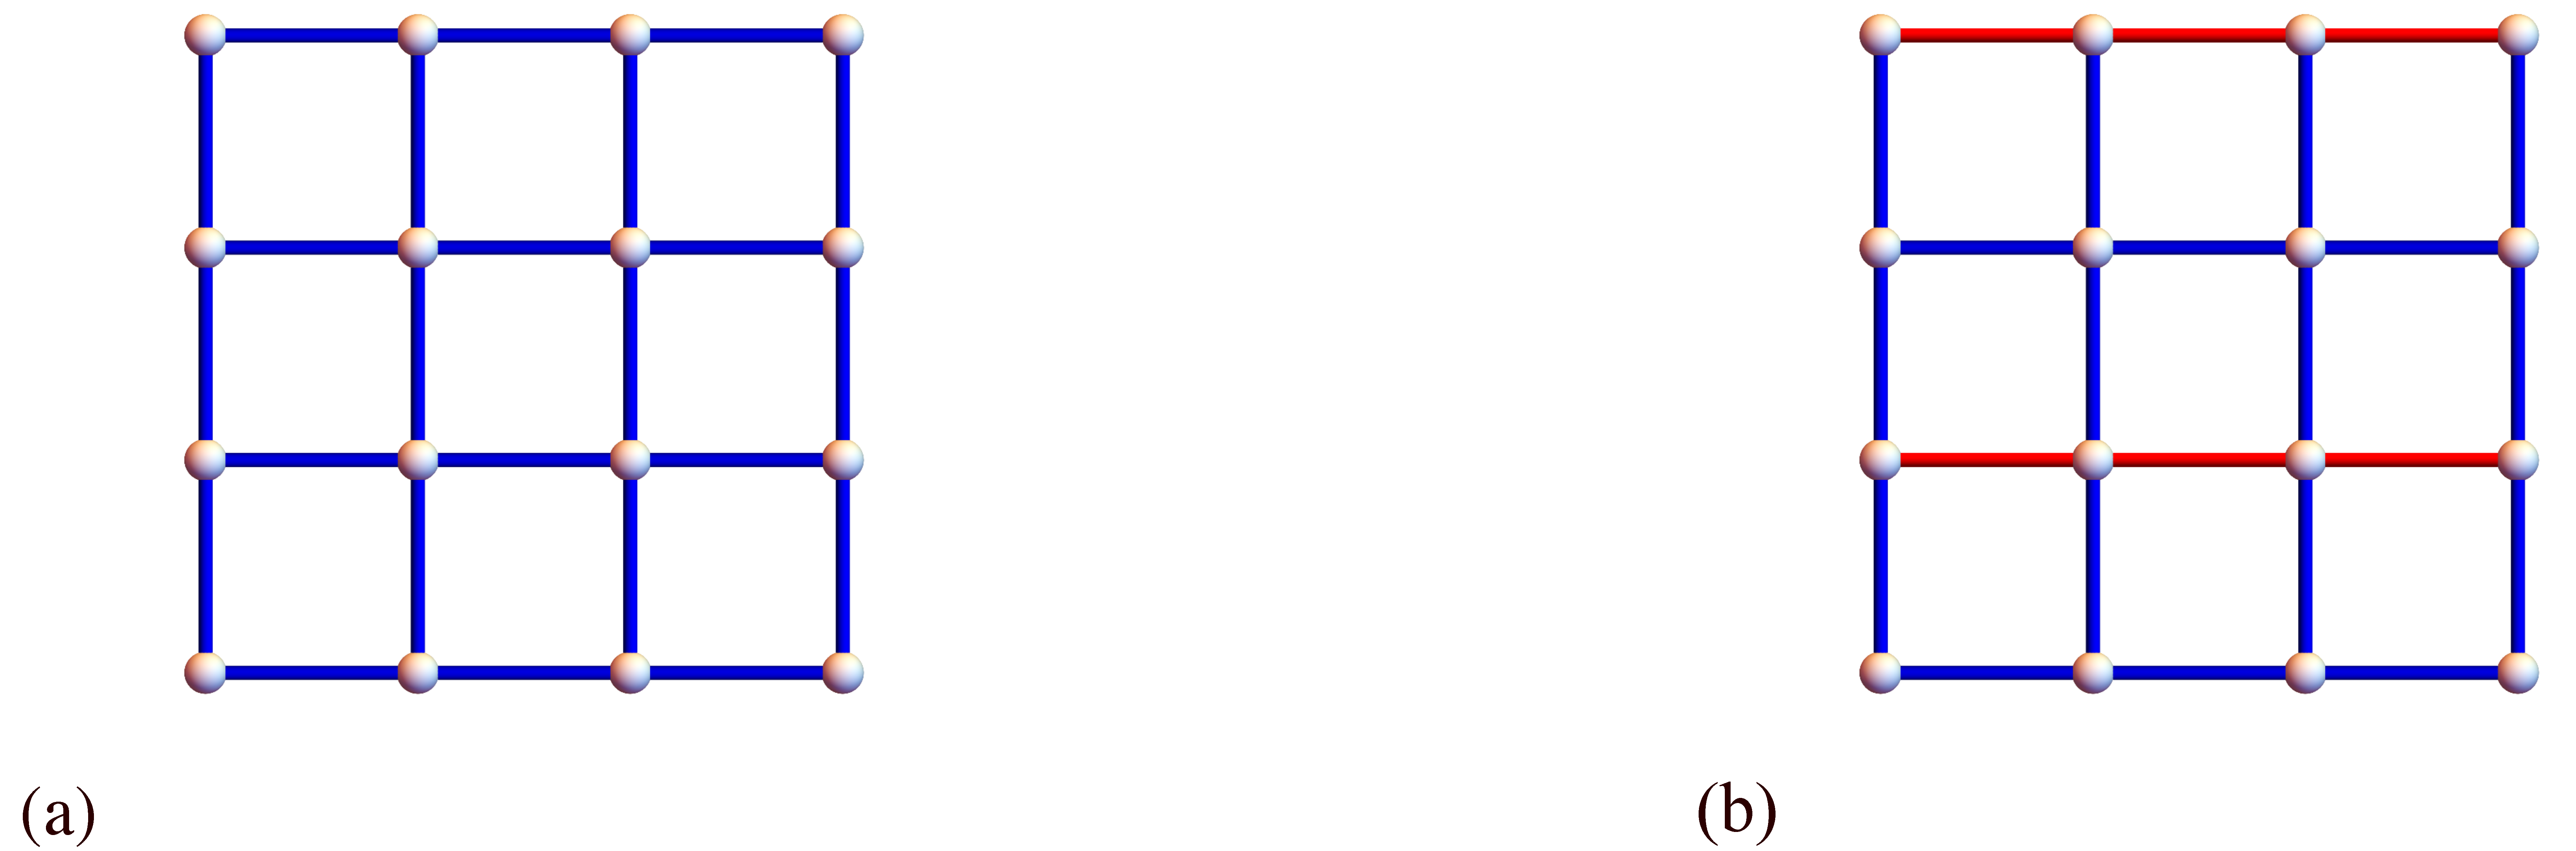
\includegraphics[width=0.8\linewidth]{./chapter04/Z2AZ2B.pdf}
	\caption{
		Visualization of the Z2A and Z2B \textit{Ans\"atze} with only nearest-neighbor couplings in (a) and (b), respectively. Blue and red colored bonds correspond to the prefactor +1 or -1, respectively, of the $U_{\bm{j}-\bm{i}}$ matrices specified by the corresponding \textit{Ansatz}.
	}
	\label{fig:chapter04_Z2AZ2B}
\end{figure}
%

Now, consider the so-called Z2B \textit{Ansatz}, which has the form~\cite{WenPLA2002}
%
\begin{equation}
	U_{\bm{i},\bm{j}} = (-1)^{(j_x-i_x) i_y} U_{\bm{j}-\bm{i}} \qquad {\rm and } \qquad A_0(\bm{i}) = 0,
\end{equation}
%
with $U_{\bm{j}-\bm{i}}$ defined as for the Z2A \textit{Ansatz} (see Figure~\ref{fig:chapter04_Z2AZ2B}~(b) for a visualization).
Translation in the $x$-direction transforms the \textit{Ansatz} as
%
\begin{align}
	\op{T}_x(U_{\bm{i},\bm{j}}) &= U_{\bm{i}-\uv{e}_x,\bm{j}-\uv{e}_x} \nonumber\\
								&= U_{\bm{i},\bm{j}}.
\end{align}
%
The corresponding gauge transformation $\op{G}_x$ is then seen to be specified by the uniform gauge transformation $G_x(i) = \tau^0$.
Translation in the $y$-direction, however, transforms the \textit{Ansatz} as
%
\begin{align}
	\op{T}_y(U_{\bm{i},\bm{j}}) &= U_{\bm{i}-\uv{e}_y,\bm{j}-\uv{e}_y} \nonumber\\
								&= (-1)^{(j_x-i_x)(i_y - 1)} U_{\bm{j}-\bm{i}} \nonumber\\
								&= (-1)^{i_x-j_x} U_{\bm{i},\bm{j}}.
\end{align}
%
Thus, the corresponding gauge transformation $\op{G}_y$ corresponds to the spatially-dependent gauge transformation $G_y(\bm{i}) = (-1)^{i_x} \tau^0$.
Note that the \textit{Ansatz} is \textit{not} invariant under translations in the $y$-direction, however, it is said to possess translation symmetry as it corresponds to a translationally invariant spin state due to the existence of the projective representation $\op{G}_y \op{T}_y$.
Additionally, the \textit{Ansatz} is seen to be invariant under global gauge transformations generated by $G_0(i) = -\tau^0$.
The projective symmetry group for the Z2B \textit{Ansatz} is then given by
%
\begin{equation}
	PSG_{\rm Z2B} = \avg{\{ \op{G}_0, \op{G}_x \op{T}_x, \op{G}_y \op{T}_y \}},
\end{equation}
%
where, to reiterate,
%
\begin{equation}
	G_0(i) = -\tau^0, \qquad G_x(i) = \tau^0, \qquad G_y(i) = (-1)^{i_x} \tau^0.
\end{equation}
%
The invariant gauge group is seen to be generated by the pure gauge transformations $\op{G}_0$, \ie,
%
\begin{equation}
	IGG_{\rm Z2B} =  \avg{\op{G}_0} \cong \ZZ.
\end{equation}
%

The \textit{Ans\"atze} Z2A and Z2B considered above are \textit{not} gauge equivalent.
Instead, they represent two \textit{distinct} \ZZ~spin liquid phases which possess all the same symmetries.
Whereas the paradigm of Landau's symmetry breaking is unable to distinguish between these two distinct quantum spin liquid phases, the projective symmetry group provides a way to probe their hidden order.
The implications of this quantum order for the low-energy excitations of the system have been glimpsed in Chapter~\ref{chapter:KitaevHoneycombModel} in the protection of Dirac fermions for the Kitaev honeycomb model.
These effects are explored further in the context of three-dimensional Kitaev spin liquids in Chapter~\ref{chapter:ClassificationOfKSL}.
As a warm-up, the following section will apply a modified form of the $SU(2)$ projective construction from Section~\ref{section:chapter04_ProjectiveConstructionOfQuantumSpinLiquids} to the Kitaev honeycomb model which has been adapted for application to Majorana fermions.


%
%%%%%%%%%%%%%%%%%%%%%%%%%%%%%%%%%%%%%%%%%%%%%%%%%%%%%%%%%%%%%%%%%%%%%%%%%%%%%%%%%%%%%%%%
\section{Application to the Kitaev honeycomb model}
\label{section:chapter04_ApplicationToTheKitaevHoneycombModel}
%%%%%%%%%%%%%%%%%%%%%%%%%%%%%%%%%%%%%%%%%%%%%%%%%%%%%%%%%%%%%%%%%%%%%%%%%%%%%%%%%%%%%%%%
%
The Kitaev honeycomb model presented in Chapter~\ref{chapter:KitaevHoneycombModel} is governed by the Hamiltonian
%
\begin{equation}
	\op{H} = -\sum_{\gamma{\rm -links}} J~\sigma^{\gamma}_j \sigma^{\gamma}_k, 
\end{equation}
%
where sites $j$ and $k$ are nearest-neighbors in the honeycomb lattice connected by a link of type $\gamma$ (refer to Chapter~\ref{chapter:KitaevHoneycombModel} for details) and the exchange couplings on all bonds have been chosen to be equal.
Substituting the spinon representation of Eq.~\eqref{eq:chapter04_SU2SpinonDefinition} into the Kitaev Hamiltonian yields the locally $SU(2)$ gauge invariant Hamiltonian
%
\begin{equation}
	\op{H} = -\frac{1}{4} \sum_{\gamma {\rm -links}} J~\trace{[F\dag_j \tau^{\gamma} F_j]} \trace{[F\dag_k \tau^{\gamma} F_k]}.
\end{equation}
%
A similar mean-field decoupling as was discussed in the previous sections for the Heisenberg model may be performed for the above Hamiltonian, however, the anisotropy of the Kitaev exchange makes for a significantly more cumbersome analysis~\cite{BurnellPRB2011}.
Instead, it has been pointed out~\cite{BurnellPRB2011,YouPRB2012,SeifertPRBFeb2018} that, given foreknowledge of the exact solution to the Kitaev model, it becomes much simpler to formulate the $SU(2)$ gauge theory in terms of Majorana fermions.

Introducing four Majorana operators at each site $c^{\gamma}$, where $\gamma = 0,x,y,z$ (the superscript for $c^0$ will be dropped for notational convenience and readability wherever it does not hinder clarity), defined in terms of the complex fermionic spinons as
%
\begin{equation}
	f_{j\uparrow} = \frac{1}{2} (c_j + ic^z_j) \qquad {\rm and } \qquad f_{j\downarrow} = \frac{1}{2} (ic^x_j - c^y_j),
\end{equation}
%
the $F$-matrices may be rewritten as
%
\begin{equation}
	F_j = \frac{1}{2} c_j^{\mu} T_{\mu},
\end{equation}
%
where $T = (\tau^0, i\tau^x, i\tau^y, i\tau^z)$.
The Majorana operators are normalized such that
%
\begin{equation}
\{c_j^{\mu}, c_k^{\nu}\} = 2\delta^{\mu\nu}\delta_{jk}.
\end{equation}
%
The spin-1/2 operators may now be expressed in terms of Majorana operators as
%
\begin{align}
	\sigma^{\gamma}_j &= \frac{1}{8} \trace{[c^{\mu}_j T\dag_{\mu} \tau^{\gamma} T_{\nu} c^{\nu}_j]} \nonumber\\
					  &= \frac{i}{4} c^{\mu}_j M^{\gamma}_{\mu\nu} c^{\nu}_j,
	\label{eq:chapter04_SpinMajoranaRepresentation}
\end{align}
%
where the three $4\times 4$ matrices
%
\begin{equation}
	M^{\gamma}_{\mu\nu} = -\frac{i}{2} \trace{[T\dag_{\mu} \tau^{\gamma} T_{\nu}]}
\end{equation}
%
form a representation of $\mathfrak{su}(2)$, \ie, $[M^{\alpha}, M^{\beta}] = 2\epsilon^{\alpha\beta\gamma} M^{\gamma}$.

For the half-filling constraint, one finds
%
\begin{equation}
	\frac{1}{2} \trace{[F_j \tau^{\gamma} F\dag_{j}]} = \frac{i}{4} c^{\mu}_j K^{\gamma}_{\mu\nu} c^{\nu}_j = 0,
	\label{eq:chapter04_HalfFillingConstraintMajorana}
\end{equation}
%
where the three $4\times 4$ matrices
%
\begin{equation}
	K^{\gamma}_{\mu\nu} = -\frac{i}{2} \trace{[T_{\mu} \tau^{\gamma} T\dag_{\nu}]}
\end{equation}
%
form another representation of $\mathfrak{su}(2)$ which, in fact, commutes with $M^{\gamma}$.
Thus, the local $SU(2)$ gauge-invariance of the Majorana representation in Eq.~\eqref{eq:chapter04_SpinMajoranaRepresentation} is seen to be generated by the matrices $K^{\gamma}$, \ie, gauge transformations take the form
%
\begin{equation}
	\bm{c}_j \rightarrow e^{\phi^{\mu}_j K^{\gamma}} \bm{c}_j,
\end{equation}
%
where $\bm{c}_j$ is the vector of Majorana operators at site $j$.
The half-filling constraint can be shown~\cite{SeifertPRBFeb2018} to reproduce the constraint $\op{D_j} = c_j c^x_j c^y_j c^z_j = 1$ for physical states as in Kitaev's original solution~\cite{KitaevAoP2006}.\footnote{The constraint here actually differs by a minus sign resulting from a choice of basis.}

With the above definitions, the Kitaev Hamiltonian may be written as a locally $SU(2)$ gauge-invariant Hamiltonian of interacting Majorana fermions
%
\begin{equation}
	\op{H} = -\frac{1}{16} \sum_{\avg{j,k}_{\gamma}} J \left(i\bm{c}\dag_j ~ M^{\gamma} ~ \bm{c}_j\right) \left(i\bm{c}\dag_k ~ M^{\gamma} ~ \bm{c}_k\right) - \frac{i}{4} \sum_j \bm{c}\dag_j ~ A_0(j) ~ \bm{c}_j,
\end{equation}
%
where $A_0(j) = \frac{1}{2} A^{\mu}_0(j) K^{\mu}$ is the temporal component of an $SU(2)$ gauge field enforcing the half-filling constraint of Eq.~\eqref{eq:chapter04_HalfFillingConstraintMajorana}.
Introducing the real Hubbard-Stratonovich matrix fields $U_{jk} = -U_{kj}$ to replace the Majorana bilinears $i c^{\mu}_j c^{\nu}_k$, the Kitaev Hamiltonian takes the form
%
\begin{equation}
	\op{H} = -\frac{J}{8} \sum_{\avg{j,k}_{\gamma}} \left(\frac{1}{2} \trace{[M^{\gamma} U_{ij} M^{\gamma} U_{ij}]} + i\bm{c}\dag_j ~ M^{\gamma} U_{ij} M^{\gamma} ~ \bm{c}_j\right) - \frac{i}{4} \sum_j \bm{c}\dag_j ~ A_0(j) ~ \bm{c}_j.
	\label{eq:chapter04_KitaevSU2}
\end{equation}
%
Hamiltonian~\eqref{eq:chapter04_KitaevSU2} is seen to describe a theory of Majorana fermions $\bm{c}_j$ coupled to a dynamic $SU(2)$ gauge field $(A_0(j), U_{jk})$, invariant under local $SU(2)$ gauge transformations $G_j = \exp{[\phi^{\mu}_j K^{\mu}]}$ as
%
\begin{align}
	\bm{c}_j	&\rightarrow G_j \bm{c}_j \nonumber\\
	A_0(j)		&\rightarrow G_j (A_0(j) + i \partial_t) G\dag_j \nonumber\\
	U_{jk}		&\rightarrow G_j U_{jk} G\dag_k.
\end{align}
%

At this stage, the zeroth order mean-field theory may be constructed by replacing the gauge field in Hamiltonian~\eqref{eq:chapter04_KitaevSU2} with a static mean-field \textit{Ansatz} $(i\ansatz{A}_0(j),~i\ansatz{U}_{jk})$ subject to the consistency conditions
%
\begin{equation}
	\ansatz{U}^{\mu\nu}_{jk} = \avg{i c^{\mu}_j c^{\nu}_k} \qquad {\rm and } \qquad \avg{\bm{c}\dag_j ~ \ansatz{A}_0(j) ~ \bm{c}_j} = 0.
\end{equation}
%
This mean-field theory may be solved to obtain the \textit{Ansatz}~\cite{YouPRB2012,SeifertPRBFeb2018}
%
\begin{equation}
	\begin{matrix*}[c]
		\ansatz{A}_0(j) 			= 0, \\
		\\
		\ansatz{U}^{\mu\nu}_{jk}	= \left\{
			\begin{matrix*}[l]
				-0.524866 &
				\qquad \text{for $\mu = \nu = 0$}\\
				1 &
				\qquad \text{for $\mu = \nu = \gamma$ and $(j,k) \in \avg{j,k}_{\gamma}$}\\
				0 &
				\qquad \text{otherwise,}
			\end{matrix*}
			\right.
	\end{matrix*}
\end{equation}
%
where a convention has been chosen such that site $j$ belongs to sublattice $A$ and site $k$ belongs to sublattice $B$.
For convenience of notation, let $u^{\mu}_{jk} = \ansatz{U}^{\mu\mu}_{jk}$, where no summation over repeated indices is implied.
Due to all $u^{\mu}_{jk}$ being unequal for any given link $\avg{j,k}$, the \textit{Ansatz} "breaks" the local $SU(2)$ gauge invariance down to a global \ZZ~gauge invariance, making the invariant gauge group \ZZ.
Note that, in agreement with the presentation of Chapter~\ref{chapter:KitaevHoneycombModel}, this mean-field \textit{Ansatz} implies the vanishing of spin-spin correlation functions beyond nearest neighbors with
%
\begin{equation}
	\avg{\sigma^{\alpha}_j \sigma^{\beta}_k} = - \delta_{\alpha\beta} \delta_{\avg{j,k}_\alpha} u^{\alpha}_{jk} u^0_{jk} = 0.524866.
\end{equation}
%

The zeroth order mean-field theory for the spin liquid may be written as
%
\begin{equation}
	\op{H} = -\frac{J}{8} \sum_{\avg{j,k}_{\gamma}} \left( i c_j u^{\gamma}_{jk} c_k + i c^{\gamma}_j u^0_{jk} c^{\gamma}_k \right) + {\rm const}.
	\label{eq:chapter04_KitaevZerothOrderMeanField}
\end{equation}
%
As a \ZZ~spin liquid, the fluctuations of the gauge field are known to be gapped and the first order mean-field theory is, thus, described by an identical Hamiltonian, albeit with the global \ZZ~gauge-invariance upgraded to a local invariance.
In fact, for the Kitaev spin liquid, the first order mean-field theory actually corresponds to the \textit{exact} solution where fluctuations of the gauge field are absent.
Diagonalization of Hamiltonian~\eqref{eq:chapter04_KitaevZerothOrderMeanField} yields three degenerate flat bands for $c^x, c^y$ and $c^z$ in addition to a graphene-like band structure for $c$ with Dirac nodes located at the $K$ and $K'$ points of the Brillouin zone~\cite{YouPRB2012,SeifertPRBFeb2018}.
The projective mean-field analysis is seen to reproduce Kitaev's original results presented in Chapter~\ref{chapter:KitaevHoneycombModel}.
With invariant gauge group $IGG = \ZZ$, the ground state of the Kitaev Hamiltonian corresponds to a stable, rigid spin liquid.

Having identified the low-energy \ZZ~theory for the Kitaev model, the projective symmetry group for the corresponding \textit{Ansatz} is considered.
The symmetry group for the Hamiltonian considered here will be $SG = \avg{\{ \op{T}_1, \op{T}_2, \op{\mathcal{P}}, \op{\mathcal{T}} \}}$, where $\op{T}_i$ generates translations along the $i^{\rm th}$ lattice vector $\ba_i$, $\op{\mathcal{P}}$ is the inversion operator and $\op{\mathcal{T}}$ is the time-reversal operator.
As varying the exchange couplings does not qualitatively affect the \textit{Ansatz} (in fact, it only changes the value of $u^0_{jk}$ for finite couplings) but \textit{does} break other lattice symmetries, \eg, rotation symmetry, these other symmetries will not be considered here.

Translation in the $\ba_1$-direction transforms the \textit{Ansatz} as
%
\begin{align}
	\op{T}_1 (i \ansatz{U}_{\bm{j}, \bm{k}})	&= i \ansatz{U}_{\bm{j}-\ba_1, \bm{k}-\ba_1} \nonumber\\
												&= i \ansatz{U}_{\bm{j}, \bm{k}}.
\end{align} 
%
The corresponding gauge transformation $\op{G}_{T_1}$ is then specified by the uniform gauge transformation $G_{T_1}(j) = \id$.
Similarly, one finds that the gauge transformation corresponding to translations in the $\ba_2$-direction is specified by the uniform gauge transformation $G_{T_2}(j) = \id$.

Inversion acts to map a bond of a given type into the same type of bond while simultaneously mapping sites from sublattice $A$ into sublattice $B$ and vice versa.
Taking advantage of translation symmetry, this action may be expressed simply as
%
\begin{align}
	\op{\mathcal{P}} (i \ansatz{U}_{\bm{j}, \bm{k}})	&= i \ansatz{U}_{\bm{k}, \bm{j}} \nonumber\\
														&= -i \ansatz{U}_{\bm{j}, \bm{k}}.
	\label{eq:chapter04_InversionOperation}
\end{align}
%
The associated gauge transformation $\op{G}_{\mathcal{P}}$ must act to cancel the minus sign in Eq.~\eqref{eq:chapter04_InversionOperation} and is seen to be specified by the spatially-dependent gauge transformation $G_{\mathcal{P}}(j) = (-1)^{\zeta_j} \id$, where
%
\begin{equation}
	\zeta_j = \left\{
		\begin{matrix*}[l]
			0 &
			\qquad \text{for $j \in$ sublattice $A$} \\
			&\\
			1 &
			\qquad \text{for $j \in$ sublattice $B$}.
		\end{matrix*}
	\right.
\end{equation}
%

The action of time-reversal on the \textit{Ansatz} is given by
%
\begin{equation}
	\op{\mathcal{T}} (i \ansatz{U}_{\bm{j}, \bm{k}}) = -i \ansatz{U}_{\bm{j}, \bm{k}}.
	\label{eq:chapter04_TimeReversalOperation}
\end{equation}
%
Similar to the inversion operation, the associated gauge transformation $\op{G}_{\mathcal{T}}$ must act to cancel the minus sign in Eq.~\eqref{eq:chapter04_TimeReversalOperation} and is seen to be specified by the spatially-dependent gauge transformation $G_{\mathcal{T}}(j) = (-1)^{\zeta_j} \id$, where $\zeta_j$ is defined as above.

The projective symmetry group for the Kitaev honeycomb model with symmetry group $SG$ is then given by
%
\begin{equation}
	PSG = \avg{\{ \op{G}_0, \op{G}_{T_1} \op{T}_1, \op{G}_{T_2} \op{T}_2, \op{G}_{\mathcal{P}} \op{\mathcal{P}}, \op{G}_{\mathcal{T}} \op{\mathcal{T}} \}},
\end{equation}
%
where $G_0(j) = -\id$ generates the invariant gauge group,
%
\begin{equation}
	G_{T_1}(j) = G_{T_2}(j) = \id \qquad {\rm and } \qquad G_{\mathcal{P}}(j) = G_{\mathcal{T}}(j) = (-1)^{\zeta_j} \id.
\end{equation}
%
As $\op{G}_\mathcal{P}$ and $\op{G}_{\mathcal{T}}$ are non-trivial, the \textit{Ansatz} is neither inversion- nor time-reversal invariant.
It is, however, both inversion and time-reversal \textit{symmetric} in the sense that it generates a physical spin state which possesses both symmetries.

Note that the gauge transformation $\op{G}_{\mathcal{T}}$ is simply a sublattice transformation.
Furthermore, as a combination of projective time-reversal and sublattice transformations, the action of $\op{\mathcal{T}}$ in the gauge-fixed sector actually corresponds to a particle-hole transformation $\op{\mathcal{C}}$ satisfying
%
\begin{equation}
	\{\op{\mathcal{C}}, \op{H}\} = 0.
	\label{eq:chapter04_ParticleHole}
\end{equation}
%
While not a property of the original spin Hamiltonian, the above relation is a property of the gauge-fixed Hamiltonian which holds true for Kitaev models with \textit{any} symmetry group.
It is merely a consequence of the Majorana representation.
Although the presence of particle-hole "symmetry" is, in this sense, trivial, the restriction it poses to the fermionic quasiparticle spectrum will be seen in the following chapter to play an important role for the low energy properties of the system.


%
%
%%%%%%%%%%%%%%%%%%%%%%%%%%%%%%%%%%%%%%%%%%%%%%%%%%%%%%%%%%%%%%%%%%%%%%%%%%%%%%%%%%%%%%%%
\section{Summary}
\label{section:chapter04_Summary}
%%%%%%%%%%%%%%%%%%%%%%%%%%%%%%%%%%%%%%%%%%%%%%%%%%%%%%%%%%%%%%%%%%%%%%%%%%%%%%%%%%%%%%%%
%
%
This chapter introduced the concept of \textit{quantum order}, an idea proposed to characterize the phases of matter to which Landau's theory of phase transitions and classical order cannot be applied.
Such phases of matter are not characterized by the spontaneous breaking of a continuous symmetry and the ideas of long-range order and local order parameters of Landau's theory are rendered inoperative.
Instead, the description of such phases requires the development of new theoretical tools.

The focus of this chapter was on one such tool called the \textit{projective symmetry group}.
The projective symmetry group was introduced in the context of classifying different quantum spin liquids with the same symmetries.
By employing a fermionic representation of spins, a spin-1/2 model may be rewritten as a fermionic model with a local $SU(2)$ gauge redundancy and analyzed using a mean-field gauge \textit{Ansatz}.
The stability of such a mean-field spin liquid depends in part upon the leftover -- and potentially reduced -- gauge redundancy of the \textit{Ansatz} which defines the so-called \textit{invariant gauge group}.
When represented in the fixed gauge sector of the mean-field spin liquid, physical symmetries must be supplemented by a gauge transformation from the invariant gauge group.
The set of all such symmetry operations acting on the mean-field spin liquid forms the projective symmetry group.
In this way, spin liquids with the same physical symmetry group are seen to possess different \textit{projective} symmetry groups and, thus, correspond to distinct spin liquid phases with different quantum order.

After a detailed discussion of these ideas, the machinery of the projective symmetry group was applied to the Kitaev honeycomb model introduced in Chapter~\ref{chapter:KitaevHoneycombModel}.
Here it was seen that the projective symmetry group is responsible for the stability of the gapless Dirac fermions in the Kitaev spin liquid.
In the next chapter, these ideas will be used to show how Kitaev spin liquids on different three-dimensional lattices may host a variety of gapless excitations, the existence of which are enforced by their unique projective symmetry groups.	% Quantum Order and Projective Symmetry Groups
%%%%%%%%%%%%%%%%%%%%%%%%%%%%%%%%%%%%%%%%%%%%%%%%%%%%%%%%%%%%%%%%%%%%%%%%%%%%%%%%%%%%%%%%
\chapter[Classification of Gapless Kitaev Spin Liquids]{Classification of Gapless\linebreak Kitaev Spin Liquids}
\label{chapter:ClassificationOfKSL}
%%%%%%%%%%%%%%%%%%%%%%%%%%%%%%%%%%%%%%%%%%%%%%%%%%%%%%%%%%%%%%%%%%%%%%%%%%%%%%%%%%%%%%%%
%
%
\footnote{This chapter discusses work which has been reported in Reference~\cite{OBrienPRB2016}.}With the work of Khaliullin and Jackeli~\cite{KhaliullinPTPS2005,JackeliPRL2009} discussed in Chapter~\ref{chapter:TransitionMetalOxides}, Kitaev's honeycomb model was upgraded from "interesting \textit{toy} model" to "analytically tractable \textit{effective} model" in the context of spin-orbit entangled Mott insulators.
The materials oriented search which it precipitated~\cite{SinghPRL2012,ChoiPRL2012,CominPRL2012,FengPRB2012,GretarssonPRL2013,GretarssonPRB2013,PlumbPRB2014,SandilandsPRL2015,KimPRB2015,MajumderPRB2015,SandilandsPRB2016,KubotaPRB2015,BanerjeeNatMat2016} produced various candidate $4d$ and $5d$ compounds such as the honeycomb materials~\sodiumIridate,~\alphaLithiumIridate~and~\ruthiniumTriChloride, which realize hexagonal arrangements of local, spin-orbit entangled $j_{\rm eff} = 1/2$ moments that are seen to be subject to strong bond-directional exchange~\cite{HwanChunNatPhys2015}.
A byproduct of this search has been the discovery of the polymorphs~\cite{TakayamaPRL2015, ModicNatComm2014}~\betaLithiumIridate~and~\gammaLithiumIridate, which realize such spin-orbit entangled moments arranged on fully three-dimensional, tricoordinated lattices.
Even more recently, there have been proposals to engineer Kitaev materials via metal-organic frameworks~\cite{MasahikoPRL2017}.

The Kitaev honeycomb model may be directly extended to spin-1/2 moments on such three-dimensional lattices and, in fact, maintains its full analytical tractability so long as the underlying lattice is tricoordinated.
Though there were earlier attempts to generalize the Kitaev model to three-dimensions for spin-3/2 moments~\cite{RyuPRB2009}, this fact was first recognized in the work of Reference~\cite{MandalPRB2009}, where the Kitaev model was solved for spin-1/2 moments on the three-dimensional hyperhoneycomb lattice.

As discussed in Chapter~\ref{chapter:KitaevHoneycombModel}, the pure Kitaev model on the \textit{two-dimensional} honeycomb lattice is known to exhibit two distinct types of quantum spin liquid ground states depending on the relative strength of the exchange couplings.
A gapped spin liquid phase is found for strongly anisotropic couplings, where both the \ZZ~fluxes and the fermionic excitations are fully gapped.
This phase hosts Abelian anyonic excitations and is known to be equivalent to the two-dimensional toric code model~\cite{KitaevAoP2003, KitaevAoP2006}.
For roughly isotropic couplings, however, there exists a gapless phase wherein the \textit{fluxes} are still gapped, but the fermions form a graphene-like dispersion with gapless Dirac nodes.

Earlier work in extending the model to three-dimensions has shown qualitatively similar ground state phase diagrams, \ie, with highly anisotropic couplings resulting in a gapped spin liquid phase, whereas isotropic couplings result in a gapless spin liquid.
In these studies, already a very rich variety physics was seen with low-energy excitations corresponding to Fermi surfaces \cite{HermannsPRB2014}, nodal lines \cite{MandalPRB2009} and topologically protected Weyl nodes \cite{HermannsPRL2015} appearing.

The work presented in this chapter goes beyond the above specific examples to provide a systematic classification of the gapless Kitaev spin liquids on two- and three-dimensional tricoordinated lattices.
This classification uses the projective symmetry group~\cite{WenPRB2002} introduced in Chapter~\ref{chapter:ProjectiveSymmetryGroup} to deduce constraints on the low-energy properties of the Kitaev Hamiltonian defined on a given lattice.
In order to illustrate the effectiveness of this idea, the Kitaev model is analyzed for a number of three-dimensional, tricoordinated lattices.

These lattices have, in fact, been comprehensively classified in the work of Wells in the 1970's \cite{Wells1977}.
However, for many of the lattices, this work marks their first appearance in the context of frustrated magnetism.
Though some lattices have been given alternative designations, following the conventions of Wells they are organized here according to their Schl\"{a}fli symbol $(p,c)$ followed by a letter, where $p$ is the polygonality (or elementary loop length), $c = 3$ refers to the tricoordination of the vertices, and the additional letter serves to enumerate the different lattices sharing a given Schl\"{a}fli symbol.
For example, the honeycomb lattice, \ie, lattice (6,3), is the unique two-dimensional tricoordinated lattice with an elementary loop length of six.
There exist three-dimensional lattices with elementary loop length 7, 8, 9 or 10 (and possibly higher).
With an eye towards realization as spin-orbit entangled iridate compounds, this work focuses on those lattices which have equal bond lengths and approximately 120$\degree$ bond angles at every vertex.

Before turning to a discussion of the classification scheme, it is necessary to make a few remarks on the solution to the Kitaev model in three-dimensions.
As was the case in two-dimensions, the Kitaev Hamiltonian
%
\begin{equation}
	\op{H}_{\rm Kitaev} = -\sum_{\gamma {\rm -links}} J_{\gamma}~\sigma^{\gamma}_j \sigma^{\gamma}_k
\end{equation}
%
may still be rewritten as a theory of Majorana fermions $c_j$ coupled to a \ZZ~gauge field $\op{u}_{jk}$ as
%
\begin{equation}
	\op{H} = i \sum_{\avg{j,k}_{\gamma}} J_{\gamma}~c_j \op{u}_{jk} c_k.
\end{equation}
%
As a result of the tricoordination of the lattices considered, the gauge field is still static and may be replaced by a fixed gauge \textit{Ansatz} corresponding to the eigenvalues $u_{jk} = \pm 1$ consistent with a ground state configuration of loop operators
%
\begin{align}
	\op{W}_p &= -\prod_{\avg{j,k} \in p} (-i \sigma^{\gamma}_j \sigma^{\gamma}_k) \nonumber\\
			 &= -i^{|p|} e^{i \op{\Phi}_p},
\end{align}
%
where $|p|$ is the length of lattice loop $p$, and $\op{\Phi}_p$ corresponds to the \ZZ~flux through that loop.
As before, Lieb's theorem~\cite{LiebHPA1992,LiebDMJ1993,LiebPRL1994} may be used to fix the canonical flux sector as the ground state whenever such a flux configuration is possible (see Chapter~\ref{chapter:KitaevHoneycombModel} for details).

One big difference in three-dimensions is the existence of volume constraints on the fluxes.
For a collection of loops in the lattice whose combination results in the boundary of a closed volume, the combined total flux in to (or out of) those loops must vanish.
As a result, not all loop operators $\op{W}_p$ corresponding to such a volume can be assigned fluxes independently.

Another consequence of these volume constraints is the existence of vison loops.
Whereas in two-dimensions, the flipping of a gauge variable results in a pair of point-like visons, flux excitations in \textit{three}-dimensions must form closed loops in order to satisfy the local volume constraints.
In two-dimensions, the flipping of successive gauge variables acts to move the visons throughout the lattice independent of one another.
However, in three-dimensions, flipping more gauge variables acts instead to increase the length of the vison loop with an energy cost proportional to the length of the loop.
This turns out to be a very important effect when studying the thermodynamics of three-dimensional Kitaev spin liquids~\cite{NasuPRL2014}.

Finally, this work additionally considers the effects of time-reversal symmetry breaking on the gapless spin liquid phases.
The concrete form of time-reversal symmetry breaking perturbation considered here is always the application of an external magnetic field in the 111-direction.
Just as in two-dimensions, the vison loops are always gapped (see Figure~\ref{fig:chapter05_VisonGaps}) and the magnetic field is assumed to be too weak to excite them.
In this case, the same effective Hamiltonian considered in Chapter~\ref{chapter:KitaevHoneycombModel} is used, \ie, the next-nearest neighbor hopping term
%
\begin{equation}
	\op{H}_{\rm eff} = \op{H}_{\rm Kitaev} + i \kappa \sum_{\avg{\avg{j,k}}} \epsilon^{\alpha\beta\gamma} u_{jl} u_{lk} c_j c_k,
\end{equation}
%
where $\kappa$ encodes the strength of the magnetic field, site $l$ is the common nearest-neighbor of sites $j$ and $k$, and $\alpha, \beta$ correspond to the bond-type connecting site $l$ to sites $j$ and $k$, respectively.

The remainder of this chapter is structured as follows.
Section~\ref{section:chapter05_Overview} gives an overview of the classification scheme developed in this work.
Section~\ref{section:chapter05_3DKitaevModels} introduces the three-dimensional lattices of interest and analyzes the corresponding Kitaev spin liquid, elaborating on details of the classification scheme as they become relevant.
In each case, the ground state phase diagram is mapped out, however, the focus of this work is always on the \textit{gapless} spin liquid phase near the point of isotropic couplings.
Section~\ref{section:chapter05_SpinPeierls} discusses related work on a possible instability for those spin liquids exhibiting full Fermi surfaces.
Finally, Section~\ref{section:chapter05_Conclusion} summarizes the systematics of the classification scheme and gives a brief outlook on future research directions.


%
%
%%%%%%%%%%%%%%%%%%%%%%%%%%%%%%%%%%%%%%%%%%%%%%%%%%%%%%%%%%%%%%%%%%%%%%%%%%%%%%%%%%%%%%%%
\section{Overview of classification via projective symmetries}
\label{section:chapter05_Overview}
%%%%%%%%%%%%%%%%%%%%%%%%%%%%%%%%%%%%%%%%%%%%%%%%%%%%%%%%%%%%%%%%%%%%%%%%%%%%%%%%%%%%%%%%
%
%
The largest symmetry group for the quantum spin liquids considered in the following classification scheme will be
%
\begin{equation}
	SG = \avg{\{ \op{T}_1, \op{T}_2, \op{T}_3, \op{\mathcal{P}}, \op{\mathcal{T}} \}}.
\end{equation}
%
All spin liquid ground states will be symmetric with respect to translation along all lattice vectors $\ba_i$.
The inversion operation $\op{\mathcal{P}}$ is, of course, only present for those lattices possessing an inversion symmetry.
The time-reversal operation $\op{\mathcal{T}}$ will be absent in the presence of explicit time-reversal symmetry breaking terms (represented here by the addition of an external magnetic field $B$ in the 111-direction) and for non-bipartite lattices which necessarily break time-reversal symmetry spontaneously.
Time-reversal symmetry is, however, present for all bipartite lattices with a pure Kitaev interaction, \ie, without a magnetic field term.
In addition to these symmetries, it is mentioned in Chapter~\ref{chapter:ProjectiveSymmetryGroup} that the Kitaev Hamiltonian represented in the Majorana basis
%
\begin{equation}
	\op{H}_{\rm Kitaev} = i \sum_{\avg{j,k}_{\gamma}} J_{\gamma}~u_{jk} c_j c_k
	\label{eq:chapter05_KitaevHamiltonianMajorana}
\end{equation}
%
is subject to an anti-unitary particle-hole transformation $\op{\mathcal{C}}$ which anti-commutes with the Hamiltonian.

With the exception of particle-hole "symmetry", all of the above symmetry operations are represented projectively in the gauge-fixed Majorana sector.
The remainder of this section considers the restrictions which different projective representations of these symmetries (combined with the particle-hole relation) put on the spectrum of a Kitaev Hamiltonian defined on a given lattice and the implications which these restrictions have for the low-energy properties of the system.


\textit{Translation symmetry}:
Due to the fact that the Kitaev model is ultimately expressed as a model of non-interacting fermions coupled to a gauge field on a lattice, Lieb's theorem guarantees that the ground state is given by the canonical flux configuration whenever possible.
As this flux configuration is determined solely by the geometry of the lattice, the ground state flux configuration will have the same translation symmetry as the underlying lattice.
With the exception of lattice (10,3)c which will be discussed in Section~\ref{section:chapter05_10_3c}, for all cases considered here, the gauge \textit{Ansatz} yielding the canonical flux configuration\footnote{The gauge \textit{Ans\"atze} considered in this chapter for lattices (8,3)c and (9,3)a do not actually correspond to the ground state of the system. The technical reasons for this will be discussed in the corresponding sections. Regardless, the gauge configurations considered in this chapter for these lattices are translationally invariant.}~is translationally invariant.
As a result, the gauge transformations $\op{G}_{T_i}$ associated to translations along the lattice vector $\ba_i$ are trivial, \ie,
%
\begin{equation}
	G_{T_i}(\br, \alpha) = 1,
\end{equation}
%
where $\br$ denotes the position of the unit cell and $\alpha$ indexes sites within the unit cell.
Since the projective symmetries associated to translations are all trivial in the above sense, the result of translation symmetry is simply the conservation of crystal momentum $\bk$, allowing the Hamiltonian matrix to be block diagonalized as $H(\bk)$.


\textit{Particle-hole symmetry}:
The presence of an anti-unitary particle-hole transformation $\op{\mathcal{C}}$ which anti-commutes with the Hamiltonian is a property of the Majorana representation used to reframe the Hamiltonian as a gauge theory.
Due to the Majorana condition $c\dag = c$, the unitary part of the particle-hole operator is just the identity and the entire operation simply corresponds to complex conjugation.
For a translationally invariant Hamiltonian such as those considered here, particle-hole symmetry implies the momentum-space relations
%
\begin{equation}
	\begin{matrix*}[l]
		H(\bk) = -H^*(-\bk) \\
		\\
		E_{\alpha}(\bk) = -E_{\beta}(-\bk),
	\end{matrix*}
\end{equation}
%
where $H(\bk)$ is the first-quantized momentum-space Hamiltonian matrix, $E_{\alpha}(\bk)$ are the corresponding eigenenergies, the asterisk indicates complex conjugation and $\alpha, \beta$ are band indices.
The latter relation reflects the fact that the complex fermionic eigenstates of the Hamiltonian satisfy $\psi\dag_{\alpha}(\bk) = \psi_{\beta}(-\bk)$.
These relations imply that the Majorana spectrum, \ie, the spectrum obtained from diagonalizing the Hamiltonian matrix of Eq.~\eqref{eq:chapter05_KitaevHamiltonianMajorana} before restriction to independent \textit{complex} fermionic states, is always anti-symmetric under inversion through $\bk = \bm{0}$.


\textit{Sublattice and time-reversal symmetries}:
All of the lattices considered here, with the exception of lattice (9,3)a, are bipartite, \ie, the lattice sites may be partitioned into two sublattices A and B such that nearest neighbors are always from different sublattices.
A consequence of the fact that the pure Kitaev Hamiltonian contains only nearest neighbor interactions is that there exists a unitary sublattice transformation which anti-commutes with the Hamiltonian.

The action of such an operator on the Majorana fermions is expressed explicitly as
%
\begin{equation}
	c_{\alpha}(\br) \mapsto {\zeta_{\alpha}(\br)}~c_{\alpha}(\br),
\end{equation}
%
where $\br$ denotes the position of the unit cell, $\alpha$ indexes sites within the unit cell and $\zeta_{\alpha}(\br)$ is defined as
%
\begin{equation}
	\zeta_{\alpha}(\br) = \left\{
		\begin{matrix*}[l]
			\phantom{-} 1 &
			\qquad \text{for $c_{\alpha}(\br) \in$ sublattice $A$} \\
			&\\
			-1 &
			\qquad \text{for $c_{\alpha}(\br) \in$ sublattice $B$.}
		\end{matrix*}
	\right.
\end{equation}
%
In the case that the sublattices have the same translation symmetry as the underlying lattice, $\zeta_{\alpha}(\br)$ is just a constant function of $\br$.
More generally, however, the sublattices are translation invariant under $\br \rightarrow \br + \ba_i + \br_0$, where $\br_0 = n_1 \ba_1 + n_2 \ba_2 + n_3 \ba_3$ with $n_i \in \{0, 1\}$ (see Figure~\ref{fig:chapter05_Sublattices} for an illustration).
In that case, $\zeta_{\alpha}(\br)$ oscillates sign with wave vector $\bk_0$ satisfying $2 \bk_0 \cdot \br_0 = 0 ~({\rm mod}~2\pi)$.
The wave vector $\bk_0$ is, thus, seen to be a superposition of reciprocal lattice vectors $\bq_i$ as $\bk_0 = (n_1 \bq_1 + n_2 \bq_2 + n_3 \bq_3)/2$.
The sublattice "symmetry" then implies the momentum-space relations
%
\begin{equation}
	\begin{matrix*}[l]
		H(\bk) = -U_{SLS}~H(\bk - \bk_0)~U\dag_{SLS}\\
		\\
		E_{\alpha}(\bk) = -E_{\beta}(\bk - \bk_0),
	\end{matrix*}
\end{equation}
%
where $U_{SLS}$ corresponds to a representation of the sublattice transformation which acts on the entire unit cell.
From these relations, the Majorana spectrum is seen to be anti-periodic in $\bk_0$ when sublattice symmetry is present.
%
\begin{figure}[tb]
	\centering
	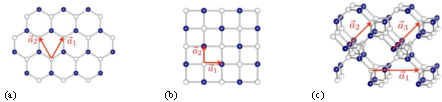
\includegraphics[width=\linewidth]{./chapter05/SublatticeSymmetry.pdf}
	\caption{
		Visualization of the A and B sublattices (in white and blue, respectively) for the (a) honeycomb, (b) square and (c) hyperhoneycomb lattices.
		While the sublattices of the honeycomb lattice have the same translation symmetry as the original lattice, the same is not true for the square and hyperoctagon lattices, leading to a non-vanishing $\bk_0$.
	}
	\label{fig:chapter05_Sublattices}
\end{figure}
%

As discussed in Chapters~\ref{chapter:KitaevHoneycombModel} and~\ref{chapter:ProjectiveSymmetryGroup}, the time-reversal operator in the Majorana sector must be supplemented by a gauge transformation $\op{G}_{\mathcal{T}}$ in order to yield a time-reversal symmetric \textit{Ansatz}.
The required gauge transformation has already been shown to be the sublattice transformation discussed above, \ie, it is specified by the (potentially) spatially-dependent gauge transformation
%
\begin{equation}
	G_{\mathcal{T}}(\br, \alpha) = \zeta_{\alpha}(\br).
\end{equation}
%
The presence of time-reversal symmetry enforces the momentum-space relations
%
\begin{equation}
	\begin{matrix*}[l]
		H(\bk) = G\dag_{\mathcal{T}}~H^*(-\bk + \bk_0)~G_{\mathcal{T}} \\
		\\
		E_{\alpha}(\bk) = E_{\beta}(-\bk + \bk_0),
	\end{matrix*}
\end{equation}
%
where $G_{\mathcal{T}}$ corresponds to a matrix representation of the gauge transformation $\op{G}_{\mathcal{T}}$ which acts on the entire unit cell, implying that the Majorana spectrum is symmetric under inversion through the point $\bk_0$.
Note that in a typical fermionic system, the time-reversal operation relates states at $\bk$ to $-\bk$, whereas the projective representation required for the gauge theory here is distinct in that it relates states at $\bk$ to $-\bk + \bk_0$.
Due to the general fact that time-reversal symmetry is the combination of particle-hole and sublattice symmetries and the fact that particle-hole symmetry is \textit{always} present in the gauge theory for the Kitaev model, both sublattice and time-reversal symmetries must always be broken simultaneously, \ie, the breaking of one implies the breaking of the other.


\textit{Inversion symmetry}:
Several lattices considered in this chapter possess inversion centers, resulting in spin liquid ground states with an inversion symmetry.
In general, the projective representation of the inversion operator has an associated gauge transformation $\op{G}_{\mathcal{P}}$.
In many cases this operator is trivial in the sense that it does not vary in space.
However, in certain cases the required gauge transformation is spatially-dependent.
Similar to the sublattice transformation, it may possess an overall sign factor which oscillates with wave vector $\til{\bk}_0 = (m_1 \bq_1 + m_2 \bq_2 + m_3 \bq_3)/2$ ($m_i \in \{0, 1\}$) as
%
\begin{equation}
	G_{\mathcal{P}}(\br, \alpha) = e^{i \til{\bk}_0 \cdot \br} G_{\mathcal{P}} (\bm{0}, \alpha).
\end{equation}
%
Note that the wave vector $\til{\bk}_0$ is distinct from the wave vector $\bk_0$ associated to time-reversal and sublattice symmetries.

The presence of inversion symmetry, thus, implies the momentum space relationships
%
\begin{equation}
	\begin{matrix*}[l]
		H(\bk) = G\dag_{\mathcal{P}}~U_{\mathcal{P}}~H(-\bk + \til{\bk}_0)~U\dag_{\mathcal{P}}~G_{\mathcal{P}} \\
		\\
		E_{\alpha}(\bk) = E_{\beta}(-\bk + \til{\bk}_0),
	\end{matrix*}
\end{equation}
%
where $U_{\mathcal{P}}$ and $G_{\mathcal{P}}$ are the matrix representations of the inversion operation $\op{\mathcal{P}}$ and the associated gauge transformation $\op{G}_{\mathcal{P}}$, respectively, which act on the entire unit cell.
The above relations imply that the Majorana spectrum is symmetric under inversion through the point $\til{\bk}_0$.
Note that in a typical fermionic system, the inversion operation relates states at $\bk$ to $-\bk$, whereas the projective representation required for the gauge theory here is distinct in that it relates states at $\bk$ to $-\bk + \til{\bk}_0$.


\textit{Effects of projective symmetries on the Majorana spectrum}:
In Section~\ref{section:chapter05_3DKitaevModels}, the Kitaev honeycomb model is extended to a number of three-dimensional, tricoordinated lattices.
In all cases, the ground state of the Kitaev Hamiltonian is a \ZZ~quantum spin liquid with gapped flux excitations.
Analogous to what is seen to occur on the honeycomb lattice in Chapter~\ref{chapter:KitaevHoneycombModel} for roughly isotropic exchange couplings, excitations above the spin liquid ground state are gapless fermions.
However, whereas in the case of the honeycomb lattice the excitations correspond to 2D Dirac fermions, the low-energy physics for the other lattices considered varies greatly, as can be seen in the overview of results provided in Table~\ref{table:chapter05_MajoranaSpectrumOverview}.
%
\begin{table}[tb]
	\centering
	\begin{tabular*}{\linewidth}{@{\extracolsep{\fill}}l|cc}
		\multirow{2}{*}{Lattice} & \multicolumn{2}{c}{Majorana spectrum} \\
		& Pure Kitaev    & TRS breaking         \\
		\hline\hline
		(10,3)a					 & Fermi surface  & Fermi surface        \\
		(10,3)b 				 & Nodal line     & Weyl nodes           \\
		(10,3)c 				 & Nodal line     & Fermi surface        \\
		\hline
		(9,3)a$^*$ 				 & Weyl nodes     & Weyl nodes           \\
		\hline
		(8,3)a  				 & Fermi surface  & Fermi surface        \\
		(8,3)b  				 & Weyl nodes     & Weyl nodes           \\
		(8,3)c$^*$ 				 & Nodal line     & Weyl nodes           \\
		(8,3)n  				 & Gapped         & Weyl nodes           \\
		\hline
		(6,3)  					 & Dirac nodes    & Gapped (non-Abelian)
	\end{tabular*}
	\caption{
		Overview of the Majorana spectrum for three-dimensional Kitaev models.
		Shown is a characterization of the nodal structure of the metallic states formed by the itinerant Majorana fermions in the gapless spin liquid phase of three-dimensional Kitaev models defined on the tricoordinated lattices of Table~\ref{table:chapter05_LatticeOverview}.
		Results for the pure Kitaev model are given in the second column.
		The third column provides information on how the nodal structure changes in the presence of an explicit time-reversal symmetry (TRS) breaking magnetic field term.
		The asterisk indicates that for these two lattices, the ground state flux sector was not used for the calculation (for details see Sections~\ref{section:chapter05_8_3c} and~\ref{section:chapter05_9_3a}).
	}
	\label{table:chapter05_MajoranaSpectrumOverview}
\end{table}
%

Although the presence or absence of individual lattice symmetries plays a role in determining the properties of the gapless excitations, it is seen to be the projective representation of those symmetries which ultimately determines the low-energy structure of the theory.
As an example, lattices (10,3)b and (8,3)b both possess sublattice and inversion symmetries, however, it is ultimately the \textit{differing} projective representations of the respective time-reversal operators which lead to lattice (10,3)b hosting a one-dimensional nodal line while lattice (8,3)b hosts isolated, topological nodal points called \textit{Weyl nodes}.
Similarly, chiral lattices (10,3)a and (10,3)c both possess sublattice symmetry but lack inversion symmetry.
However, the differing projective representations of the time-reversal operators lead to lattice (10,3)a hosting a full two-dimensional Fermi surface, whereas lattice (10,3)c hosts a one-dimensional nodal line.

The goal of this project was to determine the projective symmetry groups of the Kitaev spin liquids on a number of three-dimensional lattices corresponding to the symmetry group $SG = \avg{\{ \op{T}_1, \op{T}_2, \op{T}_3, \op{\mathcal{P}}, \op{\mathcal{T}} \}}$ and use that information to classify them according to their different PSG-protected Majorana Fermi surface topologies.
The symmetry group used in this work was chosen to represent what the authors considered to be the most fundamental symmetries and was thought to provide a complete classification of the Kitaev spin liquids.

With the benefit of hindsight and a better understanding of the ideas behind the projective symmetry group, it becomes clear that the \textit{entire} symmetry group for a given lattice should be taken into account.
Reference~\cite{YamadaPRB2017} examined Kitaev spin liquids on the three-dimensional tricoordinated lattices $8^{2}.10$-a and (10,3)d, which were not considered in the work detailed here.
Lattice $8^{2}.10$-a was shown to host a pair of three-dimensional Dirac nodes protected by a combination of fourfold-screw and and glide symmetries.
The spin liquid of lattice (10,3)d exhibits a pair of linked nodal lines protected by a combination of time-reversal and glide symmetries, one of which is stable even after time-reversal symmetry is broken.
Furthermore, Chapter~\ref{chapter:HypernonagonLattice} provides a more accurate and detailed analysis of lattice (9,3)a wherein the lattice is seen to host a nodal line phase protected by a combination of inversion and time-reversal symmetries, both of which are absent individually.
All of these possibilities are overlooked by the choice of symmetry group used here and the choice of lattices which, by chance rather than design, did not challenge such a classification scheme.

Having said that, the specific method of classification detailed here is still valid for many cases and at the very least serves to illustrate the power of the projective symmetry group as well as the richness of the physics of Kitaev spin liquids.
Many of the lattices considered here were introduced in the context of quantum magnetism for the first time through this work and it has served as a springboard for research on a variety of gapless spin liquids which had not been previously seen.

Rather than try to explain the systematic determination of Table~\ref{table:chapter05_MajoranaSpectrumOverview} in this section without the proper context, the individual ideas are explained in the next section as they become relevant.
In Section~\ref{section:chapter05_Conclusion} these principles are summarized as a coherent classification scheme.

%
\begin{figure}[p]
	\centering
	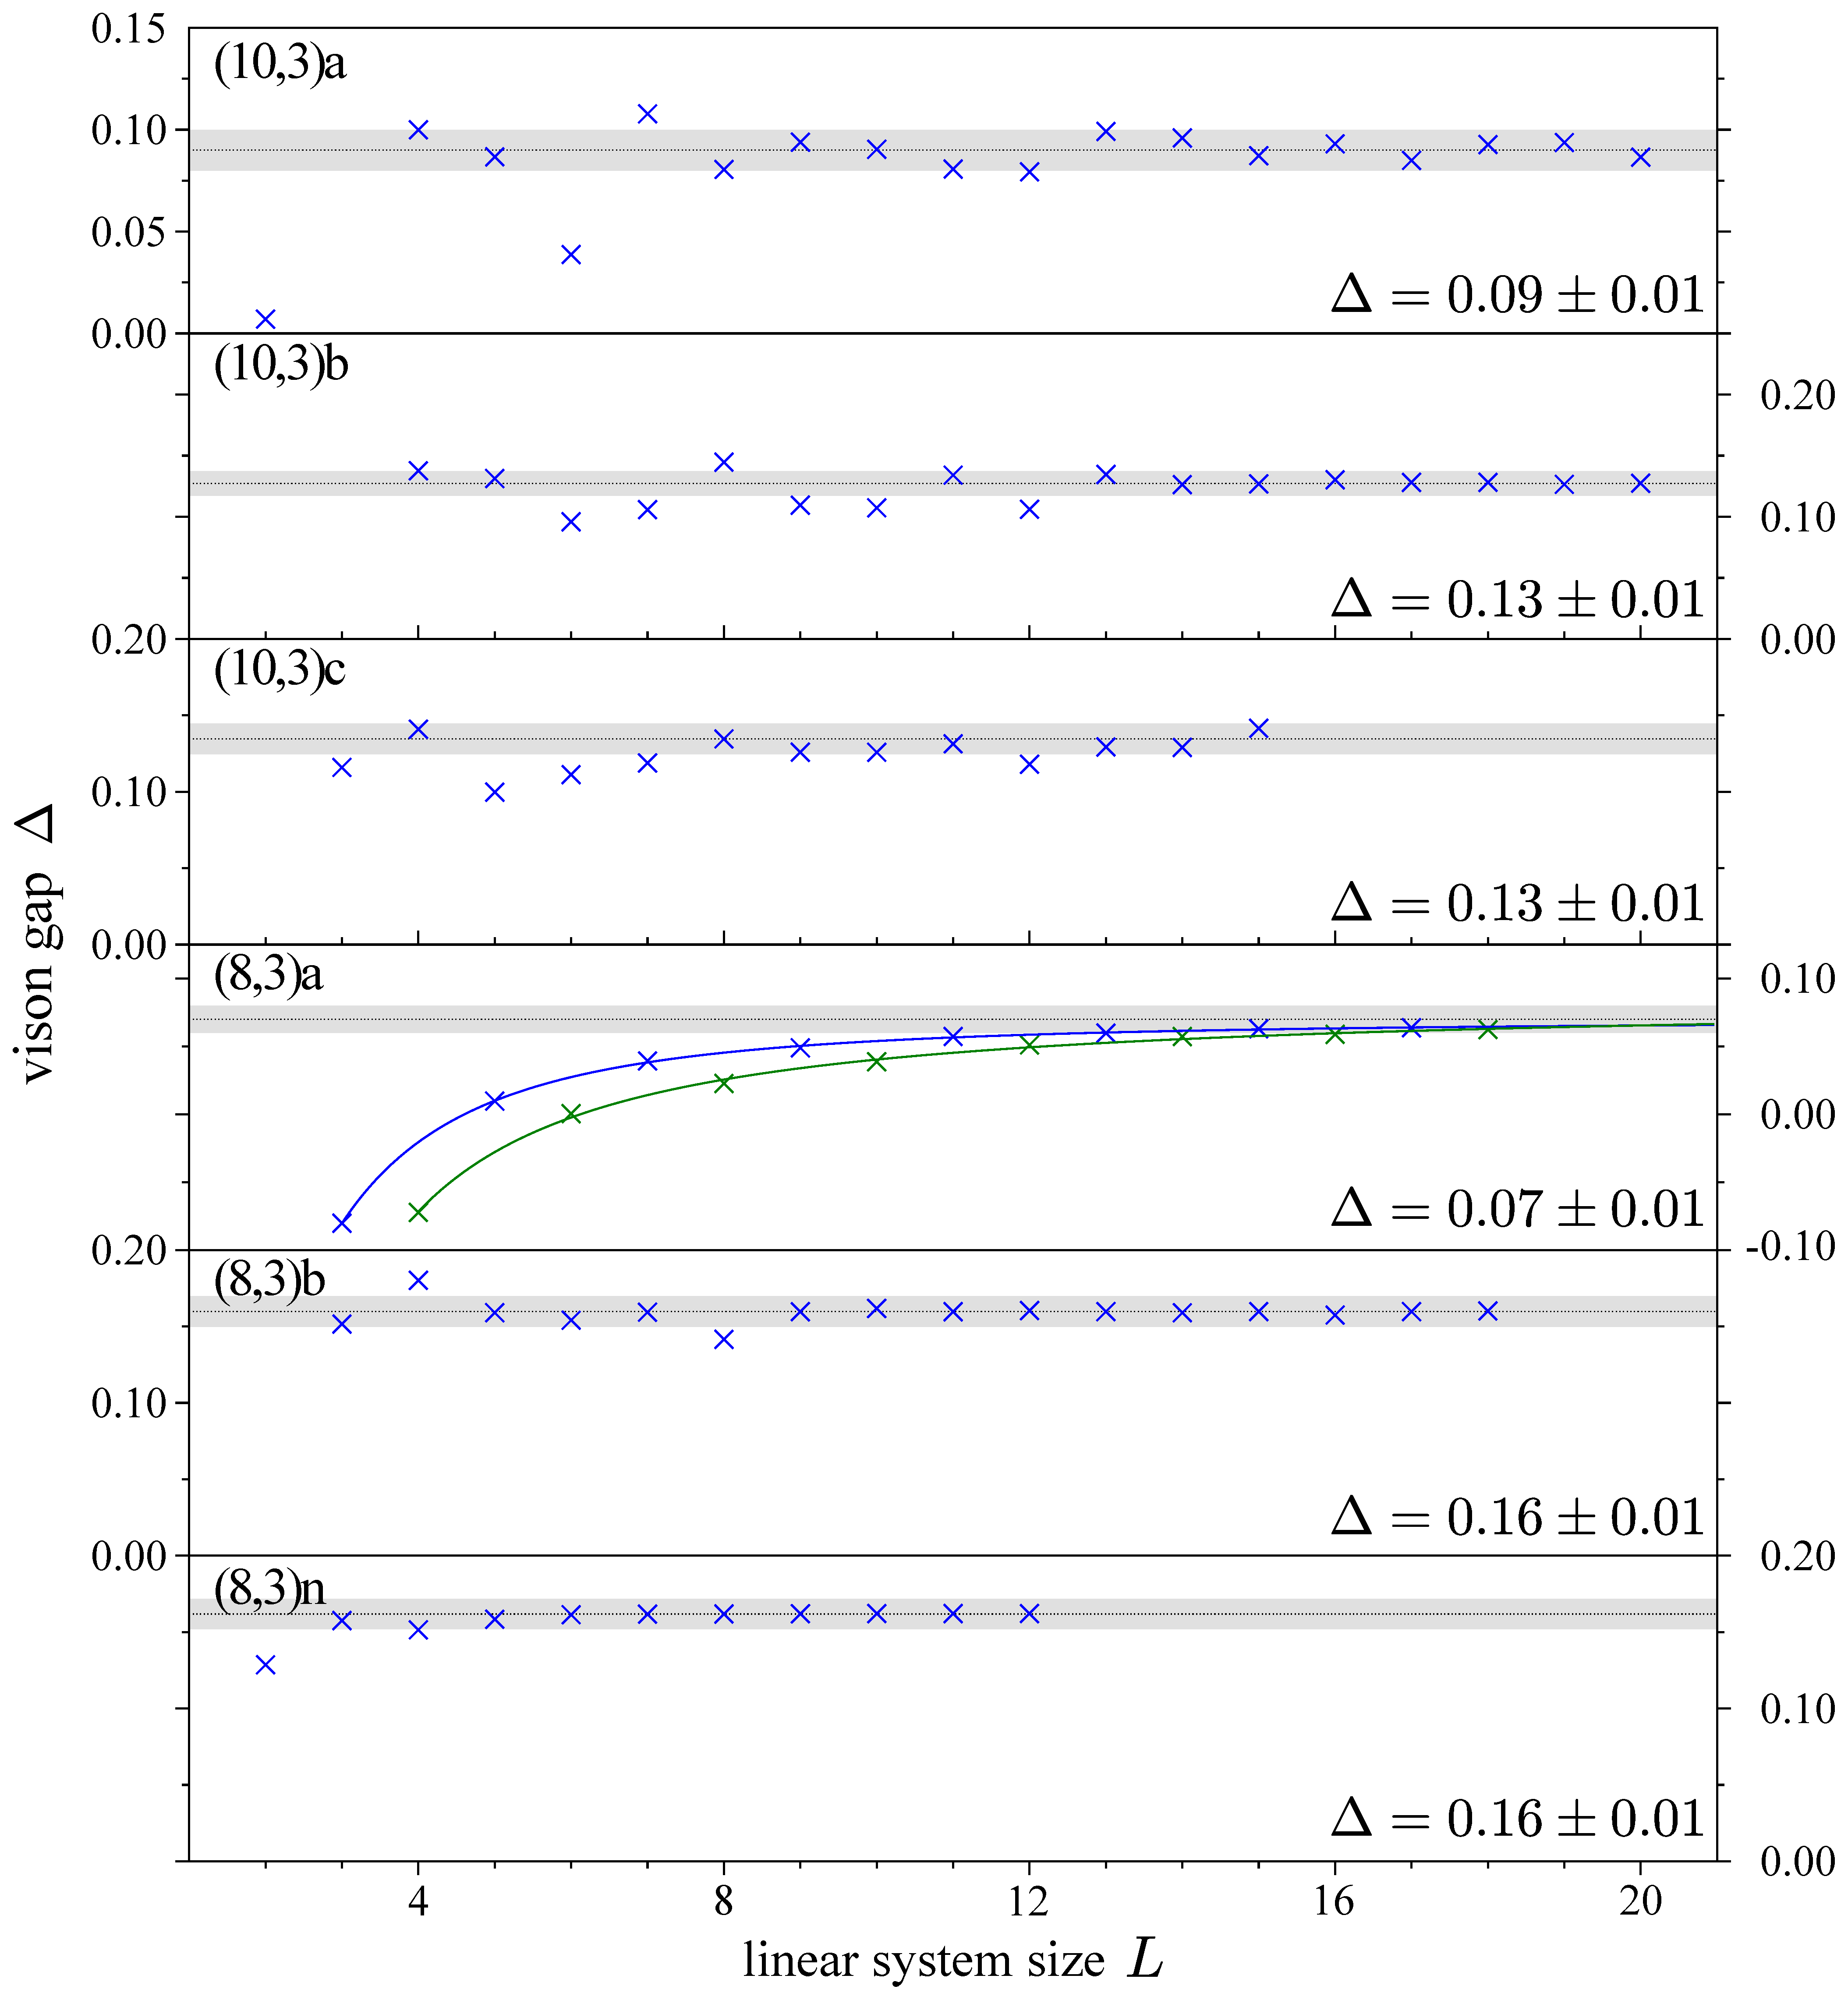
\includegraphics[width=0.95\linewidth]{./chapter05/VisonGap.pdf}
	\caption{
		Vison gap at the isotropic point obtained for the smallest vison loop as a function of system size.
		The dotted line marks the extrapolation of the gap for infinite system size, and the gray bar denotes the error of the extrapolation.
		Energies expressed in units of the exchange coupling at the isotropic point.
		Details on the vison loops can be found in Appendix~\ref{appendix:ThreeDimensionalKitaevModels}.
	}
	\label{fig:chapter05_VisonGaps}
		
	\vspace{0.5cm}

	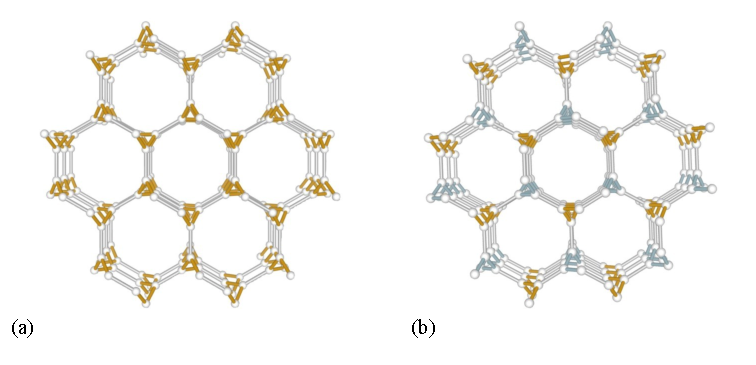
\includegraphics[width=0.7\linewidth]{./chapter05/8_3abComparison.pdf}
	\caption{
	Comparison of the co- and counter-rotating spirals of lattices (8,3)a and (8,3)b, respectively.
	The two different rotation directions are indicated by orange and blue.
	}
	\label{fig:chapter05_8_3abComparison}
\end{figure}
%

%
%\begin{figure}[p]
%	\centering
%	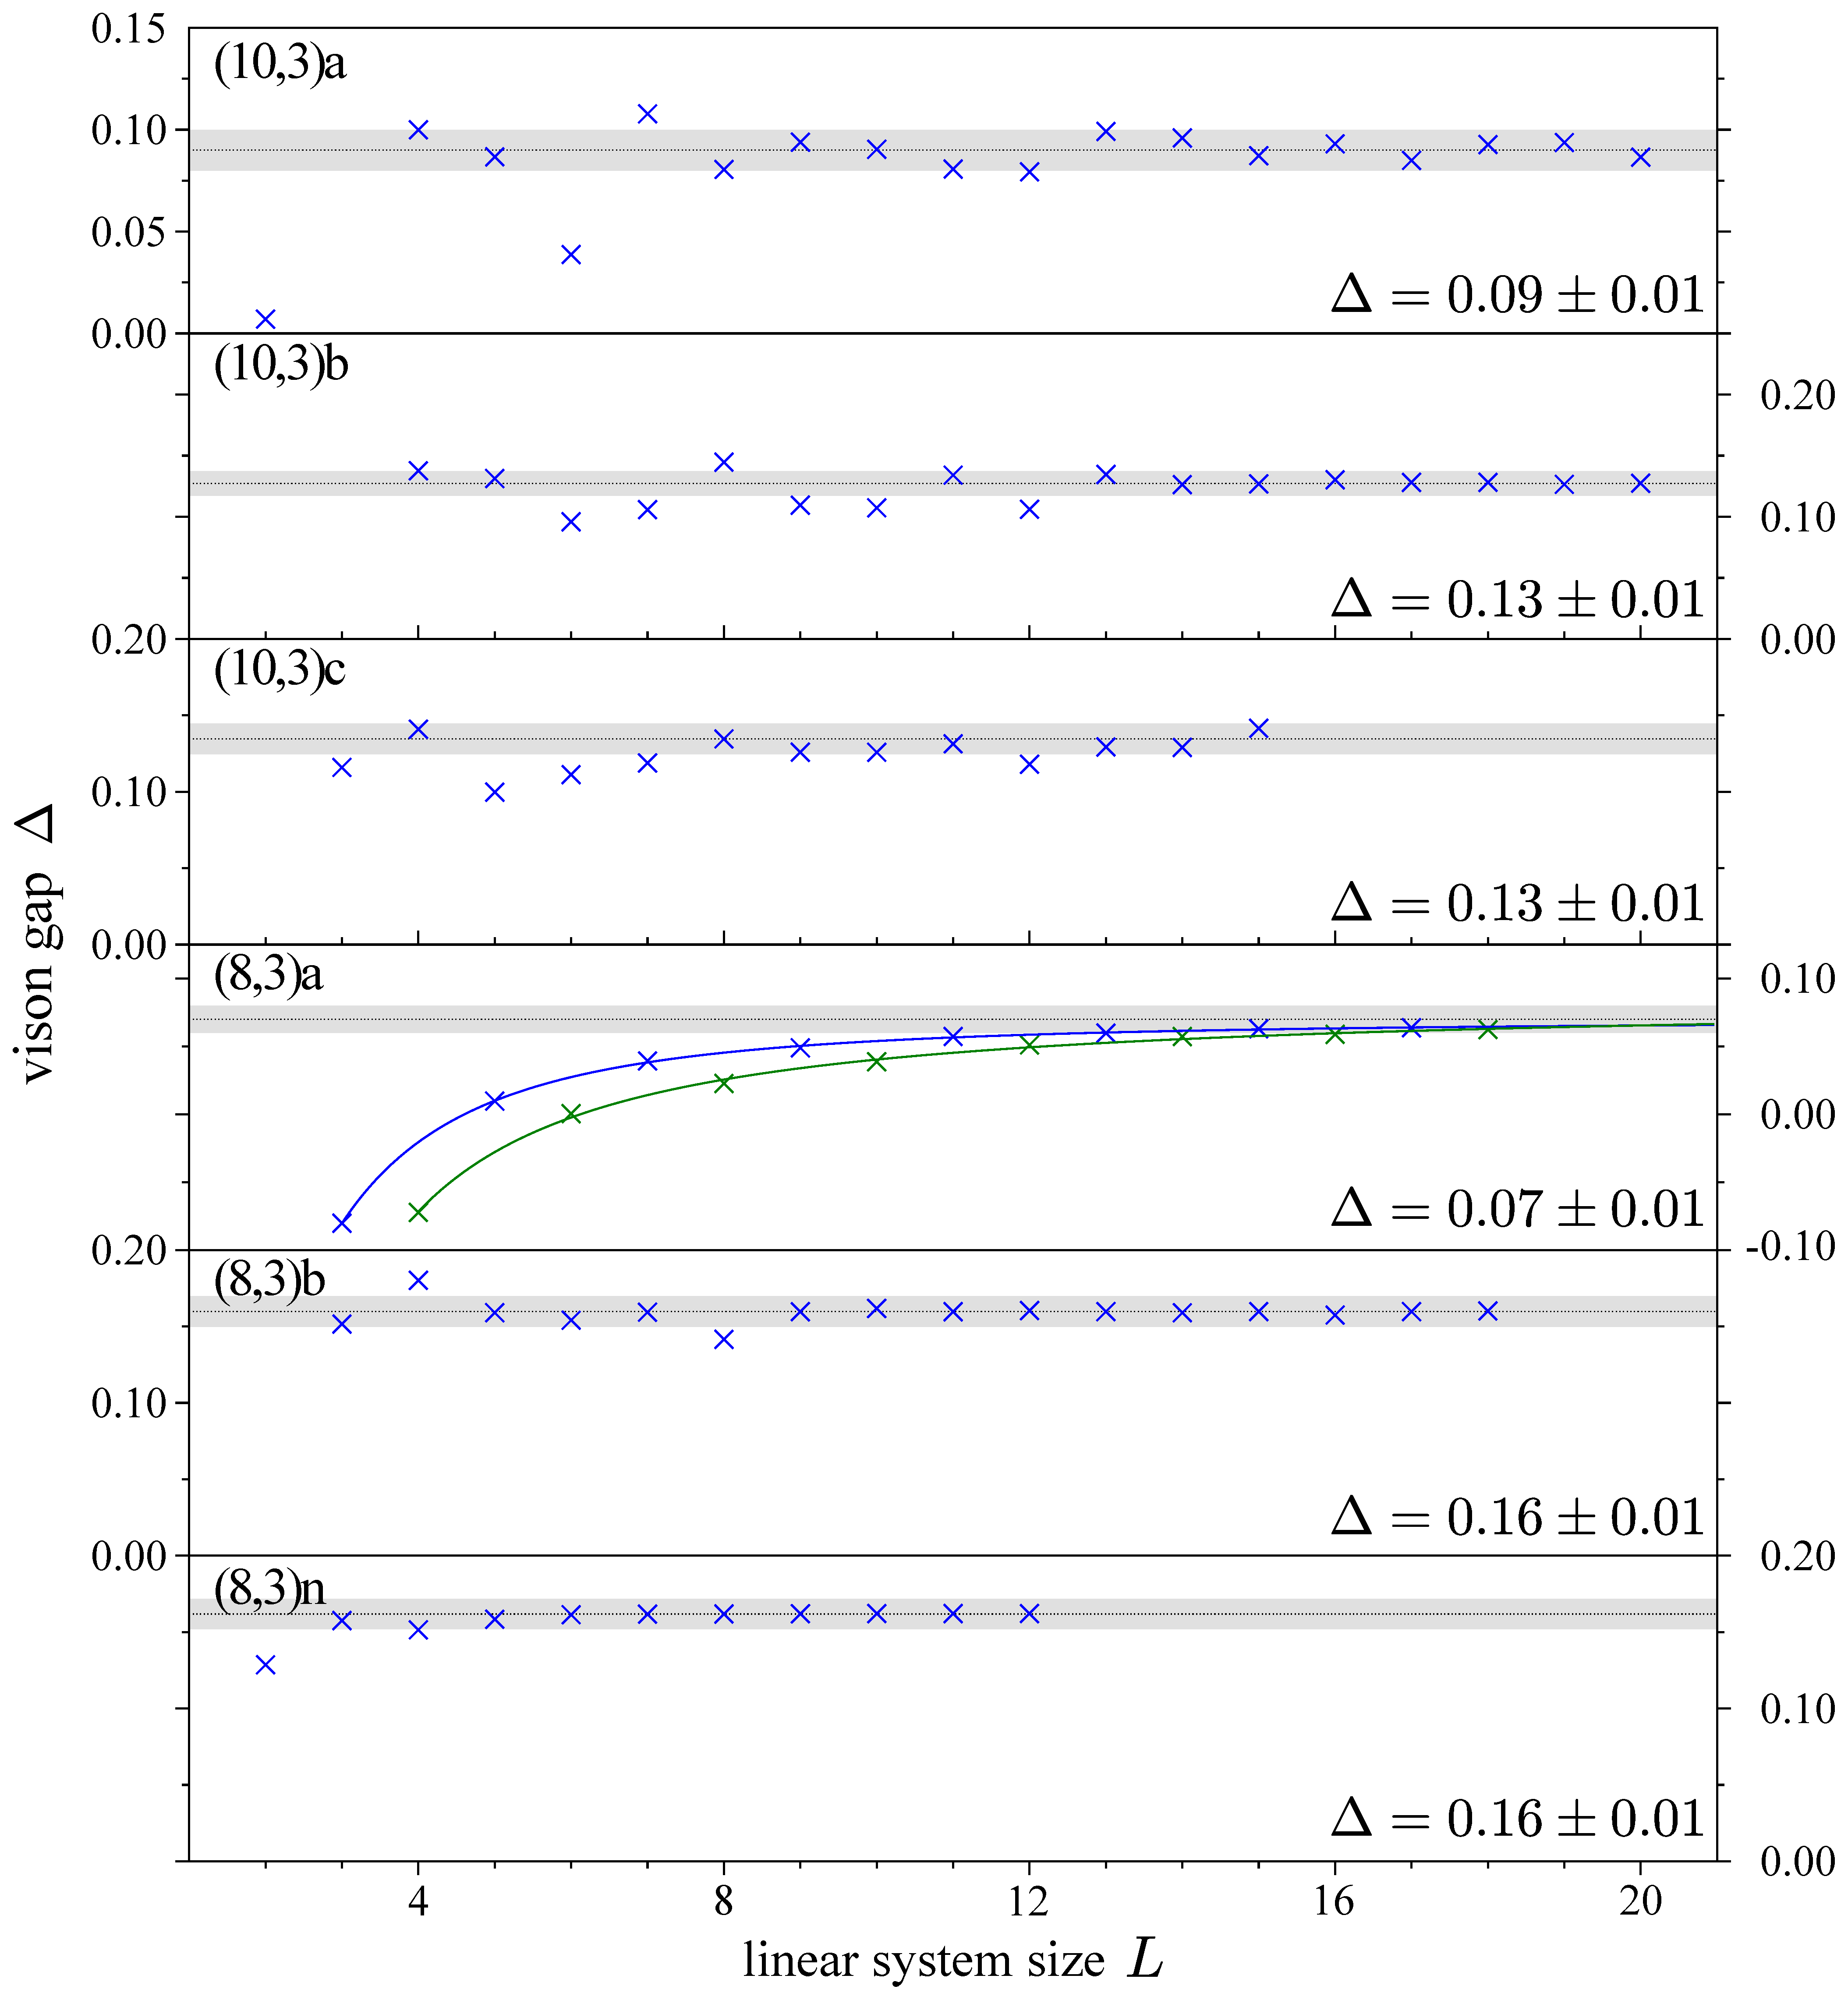
\includegraphics[width=\linewidth]{./chapter05/VisonGap.pdf}
%	\caption{
%		Vison gap obtained for the smallest vison loop as a function of system size.
%		The dotted line marks the extrapolation of the gap for infinite system size, and the gray bar denotes the error of the extrapolation.
%		Details on the vison loops can be found in Appendix~\ref{appendix:ThreeDimensionalKitaevModels}.
%	}
%	\label{fig:chapter05_VisonGaps}
%\end{figure}
%
%
%\begin{figure}[tb]
%	\centering
%	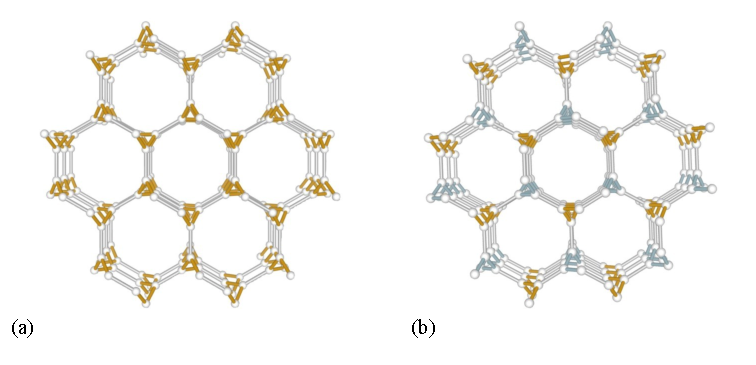
\includegraphics[width=0.8\linewidth]{./chapter05/8_3abComparison.pdf}
%	\caption{
%		Comparison of the co- and counter-rotating spirals of lattices (8,3)a and (8,3)b, respectively.
%		The two different rotation directions are indicated by orange and blue.
%	}
%	\label{fig:chapter05_8_3abComparison}
%\end{figure}
%

%
%
%%%%%%%%%%%%%%%%%%%%%%%%%%%%%%%%%%%%%%%%%%%%%%%%%%%%%%%%%%%%%%%%%%%%%%%%%%%%%%%%%%%%%%%%
\section{3D Kitaev models}
\label{section:chapter05_3DKitaevModels}
%%%%%%%%%%%%%%%%%%%%%%%%%%%%%%%%%%%%%%%%%%%%%%%%%%%%%%%%%%%%%%%%%%%%%%%%%%%%%%%%%%%%%%%%
%
%
This section introduces a number of three-dimensional tricoordinated lattices on which a Kitaev model shall be defined and provides a thorough analysis of the corresponding \ZZ~spin liquid ground state in the gapless regime.
Each lattice has a subsection dedicated to it following roughly the same pattern.
Each subsection begins by providing some elementary information about the lattice structure and the assignment of Kitaev couplings to it.
Next, the gauge structure of the corresponding gauge theory is discussed including information about the fundamental loops\footnote{Note the difference between \textit{fundamental} and \textit{elementary} loops in this context as it differs from the nomenclature of previous chapters. Here, \textit{elementary} loops are defined as the smallest closed loops in the lattice. These define the polygonality of the lattice. The \textit{fundamental} loops are defined as the smallest set of closed loops from which all other loops in the lattice may be constructed.}~of the lattice and the assignment of \ZZ~fluxes in the ground state.
What follows is a determination of the projective symmetry group and the restrictions it places on the Majorana spectrum.
Finally, a detailed analysis of the gapless Majorana spectrum is carried out.
For a brief overview of the lattices, refer to Table~\ref{table:chapter05_LatticeOverview}.
%
\begin{table}[tb]
	\centering
	\begin{tabular*}{\linewidth}{l|@{\extracolsep{\fill}}ccccc}
		Lattice 	& Sites in  & Sublattice          & Inversion                 & \multicolumn{2}{c}{Space group} \\
		& unit cell & symmetry  & symmetry            & Symbol               	  & No.      \\
		\hline\hline
		(10,3)a 	& 4         & $\bk_0 \neq \bm{0}$ & chiral                    & I$4_1 32$            & 214      \\
		(10,3)b 	& 4         & \checkmark          & \checkmark                & Fddd                 & 70       \\
		(10,3)c 	& 6         & \checkmark          & chiral                    & P$3_1 12$            & 151      \\
		\hline
		(9,3)a  	& 12        & ---                 & \checkmark                & R$\overline{3}$m     & 166      \\
		\hline
		(8,3)a  	& 6         & $\bk_0 \neq \bm{0}$ & chiral                    & P$6_2 22$            & 180      \\
		(8,3)b  	& 6         & $\bk_0 \neq \bm{0}$ & \checkmark                & R$\overline{3}$m     & 166      \\
		(8,3)c  	& 8         & \checkmark          & \checkmark                & P$6_3$ / mmc         & 194      \\
		(8,3)n  	& 16        & \checkmark          & $\til{\bk}_0 \neq \bm{0}$ & I4 / mmm             & 139      \\
		\hline
		(6,3)   	& 2         & \checkmark          & \checkmark                &                      &         
	\end{tabular*}
	\caption{
		Overview of elementary tricoordinated lattices in (mostly) three spatial dimensions.
		Following the classification of A.~F. Wells~\cite{Wells1977}, the lattices considered here are of fixed polygonality $p$, \ie, a fixed length of all elementary closed loops, and vertex coordination $c=3$ using the Schl\"afli symbol $(p,c)$ followed by a letter.
		Basic information is listed for each lattice including the number of lattice sites $Z$ in the unit cell, whether the lattice exhibits (non-trivial) sublattice and/or inversion symmetries, as well as information about the space group.
	}
	\label{table:chapter05_LatticeOverview}
\end{table}
%


%
%
% LATTICE (8,3)A %%%%%%%%%%%%%%%%%%%%%%%%%%%%%%%%%%%%%%%%%%%%%%%%%%%%%%%%%%%%%%%%%%%%%%%
\subsection{Lattice (8,3)a}
\label{section:chapter05_8_3a}
%%%%%%%%%%%%%%%%%%%%%%%%%%%%%%%%%%%%%%%%%%%%%%%%%%%%%%%%%%%%%%%%%%%%%%%%%%%%%%%%%%%%%%%%
%
%
\subsubsection{Lattice information}
%
%
The first lattice to be considered is (8,3)a.
The lattices (8,3)a and (8,3)b (Section~\ref{section:chapter05_8_3b}) are, in a sense, related.
Both may be viewed as a three-dimensional version of the 3-12-12~\cite{YangPRB2007} or Yao-Kivelson lattice~\cite{YaoPRL2007}, with the triangles replaced by triangular spirals.
Whereas the spirals of lattice (8,3)a are co-rotating, resulting in a chiral lattice, those of lattice (8,3)b are counter-rotating, yielding an inversion-symmetric lattice (refer to Figure~\ref{fig:chapter05_8_3abComparison} for a comparison).

More formally, lattice (8,3)a is specified by the hexagonal space group $P6_{2}22$ (No. 180) with $c/a = 3\sqrt{2}/5$ and Wyckoff positions for the unit cell are $6(i)$ with $x=2/5$.
The concrete choice of six site unit cell used in this work is given by the site positions
%
\begin{equation}
	\begin{matrix*}[l]
		\br_1 = \left(\frac{1}{2}, \frac{\sqrt{3}}{10}, 0\right) &
		\br_2 = \left(\frac{3}{5}, \frac{\sqrt{3}}{5}, \frac{2\sqrt{2}}{5}\right) &
		\br_3 = \left(\frac{1}{10}, \frac{3\sqrt{3}}{10}, \frac{\sqrt{2}}{5}\right) \\
		&\\
		\br_4 = \left(\frac{2}{5}, \frac{\sqrt{3}}{5}, \frac{\sqrt{2}}{5}\right) &
		\br_5 = \left(0, \frac{2\sqrt{3}}{5}, 0\right) &
		\br_6 = \left(-\frac{1}{10}, \frac{3\sqrt{3}}{10}, \frac{2\sqrt{2}}{5}\right).
	\end{matrix*}
\end{equation}
%
The lattice vectors are chosen to be
%
\begin{equation}
	\begin{matrix*}[l]
		\ba_1 = (1, 0, 0) \qquad
		\ba_2 = \left(-\frac{1}{2}, \frac{\sqrt{3}}{2}, 0\right) \qquad
		\ba_3 = \left(0, 0, \frac{3\sqrt{2}}{5}\right)
	\end{matrix*}
\end{equation}
%
with the corresponding reciprocal lattice vectors
%
\begin{equation}
	\begin{matrix*}[l]
		\bq_1 = \left(2\pi, \frac{2\pi}{\sqrt{3}}, 0\right) \qquad
		\bq_2 = \left(0, \frac{4\pi}{\sqrt{3}}, 0\right) \qquad
		\bq_3 = \left(0, 0, \frac{5\sqrt{2}\pi}{3}\right).
	\end{matrix*}
\end{equation}
%

The unit cell and translation vectors are illustrated in Figure~\ref{fig:chapter05_8_3aPanel}~(a).
The bonds in the figure are colored red, green and blue to indicate the assignment of $x$-, $y$- and $z$-type bonds, respectively.
This assignment of bonds is chosen to respect as many of the lattice symmetries as possible and is unique up to an overall permutation of the three bond types.
More specifically, there are two distinct sets of $x$-, $y$- and $z$-bonds which cannot be related by symmetries, namely, those which compose the co-rotating spirals and those which connect neighboring spirals.
All bonds in a given set, however, are related by a combination of a $C_2$ rotation and a threefold screw axis.
The symmetry between $x$-, $y$- and $z$-bonds is reflected in the ground state phase diagram shown in Figure~\ref{fig:chapter05_8_3aPanel}~(b).


%
%
\subsubsection{Gauge structure}
%
%
Lattice (8,3)a possesses three loop operators of length 8 and three of length 14 per unit cell.
These six loop operators may be combined to form three closed volumes leading to only \textit{three} independent loop operators per unit cell (see Appendix~\ref{appendix:ThreeDimensionalKitaevModels_8_3a} for details).
The canonical flux sector for lattice (8,3)a corresponds to $\pi$-flux through all loops of length 8 and $0$-flux through all loops of length 14.
This results in all loop operators $\op{W}_p$ having eigenvalue +1.
Additionally, it has been checked numerically that the canonical flux sector is, indeed, the ground state flux sector.
The vison gap for lattice (8,3)a shown in Figure~\ref{fig:chapter05_VisonGaps}~and Table~\ref{table:chapter05_VisonGaps}~has been computed by flipping the value of $u_{jk}$ for a single $z$-bond, resulting in the excitation of four loop operators (further details are given in Appendix~\ref{appendix:ThreeDimensionalKitaevModels_8_3a}).
%
\begin{table}[tb]
	\centering
	\begin{tabular*}{\linewidth}{l|@{\extracolsep{\fill}}ccc}
		Lattice     & Flux sector    & Vison gap & Vison loop length \\
		\hline\hline
		(10,3)a     & $0$-flux       & 0.09(1)   & 10                \\
		(10,3)b     & $0$-flux       & 0.13(1)   & 6                 \\
		(10,3)c     & $0$-flux       & 0.13(1)   & 3                 \\
		\hline
		(9,3)a$^*$  & $\pi/2$-fluxes & ---       & 4                 \\
		\hline
		(8,3)a      & $\pi$-flux     & 0.07(1)   & 2                 \\
		(8,3)b      & $\pi$-flux     & 0.16(1)   & 2                 \\
		(8,3)c$^*$  & $0$-flux       & ---       & 4                 \\
		(8,3)n      & $\pi$-flux     & 0.16(1)   & 2                 \\
		\hline
		(6,3)       & $0$-flux       & 0.27      & ---                
	\end{tabular*}
	\caption{
		Overview of the physics of the \ZZ~gauge field for three-dimensional Kitaev models.
		The second column provides the flux assignment of the \textit{elementary} loops for the Kitaev model defined on the lattices in the first column.
		The third column gives the size of the vison gap for isotropic couplings in units of the exchange coupling, whereas the fourth column provides the length of the smallest vison loop in terms of the number of excited \textit{elementary} loop operators.
		The asterisk indicates that for these two lattices, the results provided do not correspond to the ground state flux sector.
	}
	\label{table:chapter05_VisonGaps}
\end{table}
%


%
%
\subsubsection{Projective symmetries}
%
%
Lattice (8,3)a is bipartite with different sublattices connected by the vector $\br_0 = \ba_3$.
As a result, the projective representation of time-reversal is given by
%
\begin{equation}
	H(\bk) = G\dag_{\mathcal{T}}~H(-\bk + \bk_0)~G_{\mathcal{T}},
\end{equation}
%
where $\bk_0 = \bq_3/2$ and the associated gauge transformation matrix is given by
%
\begin{equation}
	G_{\mathcal{T}} =
		\begin{pmatrix}
			\id & 0 \\
			0	& -\id
		\end{pmatrix}.
\end{equation}
%
As lattice (8,3)a is chiral, the only other restriction to consider is that of particle-hole symmetry.
The resulting energy relations are given by\pagebreak
%
\begin{equation}
	E_{\alpha}(\bk) = -E_{\beta}(-\bk) \qquad {\rm and } \qquad E_{\alpha}(\bk) = E_{\gamma}(-\bk + \bk_0),
\end{equation}
%
due to particle-hole and time-reversal symmetry, respectively.
Due to the fact that the gauge transformation $\op{G}_{\mathcal{T}}$ relates states at momentum $\bk$ to states at momentum $\bk - \bk_0$, the momentum space Hamiltonian matrix has the general form
%
\begin{equation}
	H(\bk) = 
		\begin{pmatrix}
			0			&			& A(\bk) 	\\
						& \ddots 	& 			\\
			A\dag(\bk)	&			& 0
		\end{pmatrix},
	\label{eq:chapter05_8_3aGenericHamiltonian}
\end{equation}
%
\ie, other than being skew-symmetric (due to the Majorana condition), it is a generic band Hamiltonian.


%
%
\subsubsection{Majorana band structure}
%
%
Given the general form of the Kitaev Hamiltonian in Eq.~\eqref{eq:chapter05_8_3aGenericHamiltonian} for lattice (8,3)a, zero modes at a given momentum correspond to a vanishing determinant of the Hamiltonian matrix $H(\bk)$.
In three-dimensions, solutions of $\det{H(\bk)} = 0$ correspond to a two-dimensional manifold of $\bk$-points.
The conclusion is that for the Kitaev model defined on lattice (8,3)a, the only stable zero-energy manifolds are \textit{Fermi surfaces}.

The fact that lattice (8,3)a has non-vanishing $\bk_0$ associated to the projective time-reversal operation while also lacking inversion symmetry implies the lack of an energy relation such as $E_{\alpha}(\bk) = -E_{\beta}(\bk)$.
A consequence of this lack of symmetry at a fixed momentum is that an isolated band may cross the Fermi energy, resulting in the formation of a Fermi surface.

Such a situation is even more interesting in the presence of degeneracies in the Majorana spectrum.
In the absence of symmetries, the spectrum of a generic band Hamiltonian may have degeneracies corresponding to bands $E_{+}(\bk)$ and $E_{-}(\bk)$ at isolated momenta $\bk^*$, described locally by
%
\begin{equation}
	E_{\pm} (\bk) \approx E_0(\bk^*) \pm \sum_i~b^{i}_{\pm} |k_{i} - k^*_{i}| \qquad {\rm where } \qquad b^{i}_{\pm} \in \mathbb{R}_{+}.
\end{equation}
%
For non-vanishing $E_0(\bk^*)$, the band $E_{-}$ may cross the Fermi energy resulting in a Fermi surface which may be gapped out only if the degeneracy is lifted.
Such a degeneracy is a topological property of the Hamiltonian with a robust topological charge (chirality) associated to it.
As such, these degeneracies may only be lifted by being brought into contact with another degeneracy of the opposite topological charge and mutually annihilating.\footnote{If interactions are allowed, however, degeneracies may be coupled non-locally in momentum space. Regardless, the interactions must couple degeneracies of opposite charge.}
Note that particle-hole symmetry guarantees the existence of a degeneracy with opposite topological charge located at $-\bk^*$ and with energy $E_0(-\bk^*) = -E_0(\bk^*)$.
As a result, the Fermi surface inherits a topological protection from the associated degeneracy.
Such degeneracies are closely related to the massless Weyl nodes which will be discussed in greater detail in Section~\ref{section:chapter05_8_3b}.
%
\begin{figure}[tb]
	\centering
	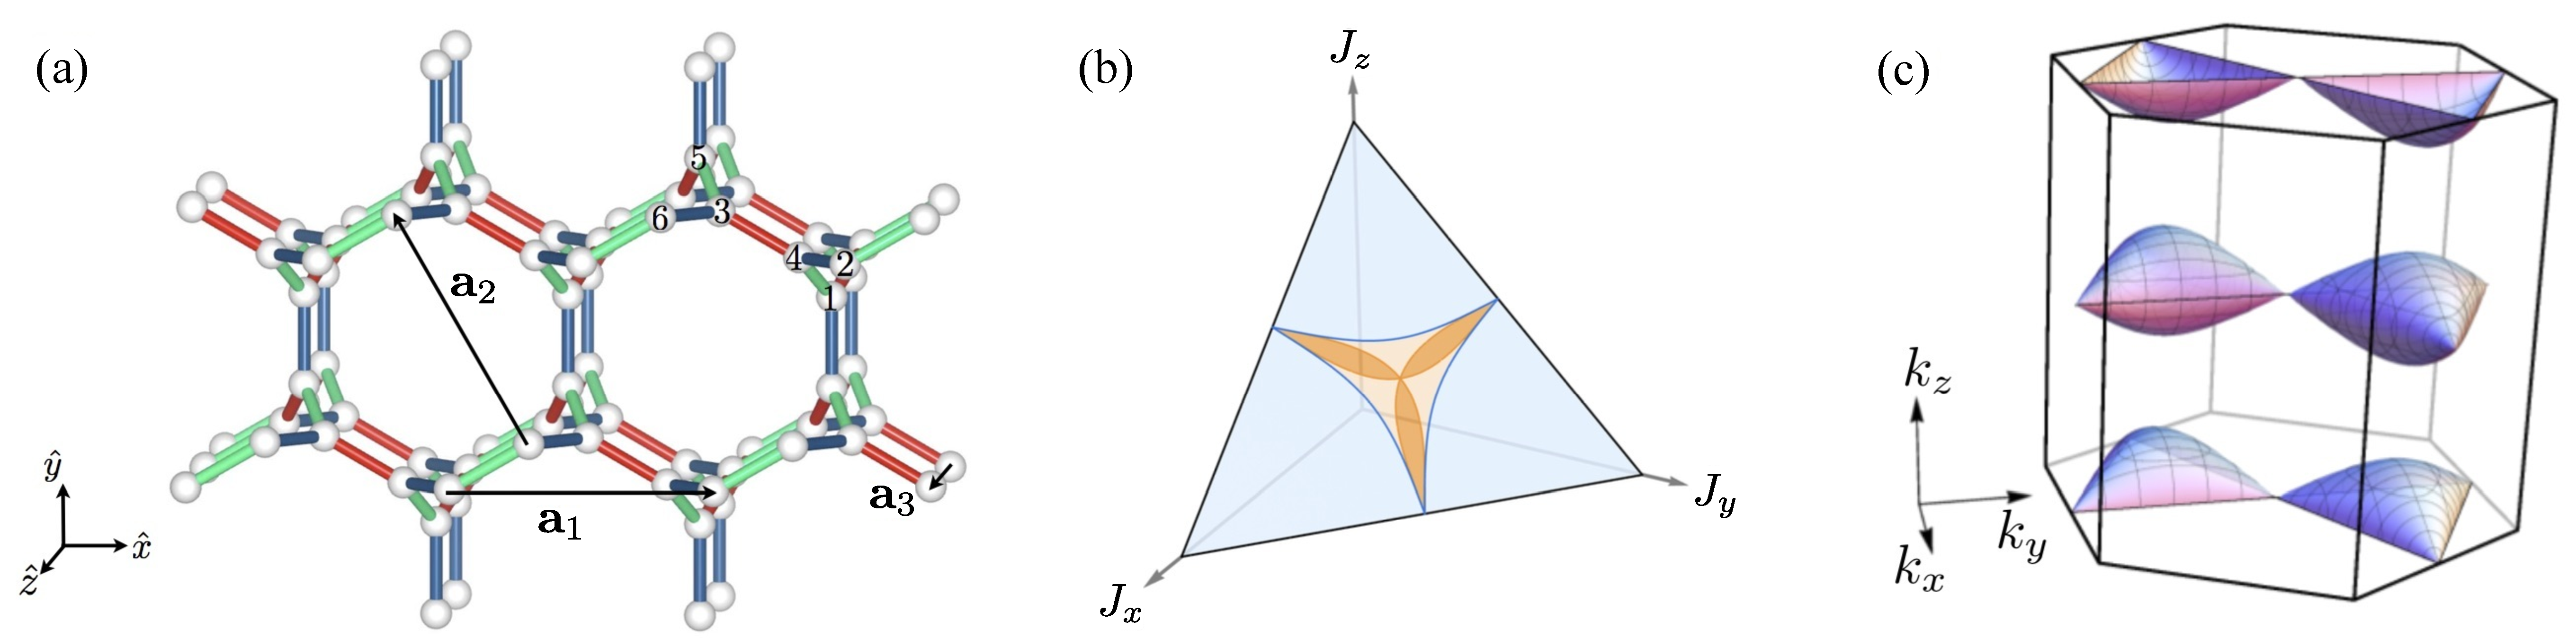
\includegraphics[width=\linewidth]{./chapter05/8_3aPanel.pdf}
	\caption{
		(a) Unit cell and translation vectors for the Kitaev model on lattice (8,3)a.
		(b) Ground state phase diagram for lattice (8,3)a.
		The regions shaded darker orange have topological Fermi surfaces while the lighter orange regions have topologically-trivial Fermi surfaces.
		The blue shaded regions are gapped.
		(c) Visualization of the four Majorana Fermi surfaces for isotropic exchange couplings.
	}
	\label{fig:chapter05_8_3aPanel}
\end{figure}
%

Diagonalizing the concrete Kitaev Hamiltonian for lattice (8,3)a reveals an extended gapless phase around the point of isotropic exchange couplings (see phase diagram in Figure~\ref{fig:chapter05_8_3aPanel}~(b)), where the zero modes correspond to the Majorana Fermi surfaces visualized in Figure~\ref{fig:chapter05_8_3aPanel}~(c).
The darker orange shaded regions of the phase diagram denote the parameter space where the Majorana Fermi surfaces are topologically protected, \ie, they are generated by a topological degeneracy as discussed above.
These degeneracies can be seen in the energy dispersion in Figure~\ref{fig:chapter05_8_3aDispersion}~(b).
For isotropic couplings, oppositely charged topological degeneracies are located at $\bk^* = \pm (\frac{\pi}{3}, \frac{\pi}{\sqrt{3}}, 0)$ and at $-\bk^* + \bk_0$ corresponding to their time-reversal partners.
Note that the act of time-reversal yields topological degeneracies of the \textit{same} charge and energy (see discussion of Weyl nodes in Section~\ref{section:chapter05_8_3b}).
Additionally, there are topologically neutral degeneracies located at the touching points of the different Fermi surfaces.
These topologically neutral points correspond to pairs of oppositely charged degeneracies sitting on top of one another.

As can be seen in Figure~\ref{fig:chapter05_8_3aPanel}~(c), pairs of Majorana Fermi surfaces are related by the nesting vector $\bk_0$, suggesting a Fermi surface instability for the case of \textit{interacting} Majorana fermions.
Interactions between Majorana fermions are introduced as soon as any other type of magnetic exchange is added to the pure Kitaev Hamiltonian, thus, such a possible instability becomes important for any realistic model.
A very similar situation occurs in the (10,3)a hyperoctagon lattice (see Section~\ref{section:chapter05_10_3a}) and was studied in Reference~\cite{HermannsPRL2015b}.
Details of this so-called \textit{spin-Peierls instability} are discussed in Section~\ref{section:chapter05_SpinPeierls}.
Breaking time-reversal symmetry by applying an external magnetic field does not qualitatively change the nature of the nodal manifold, \ie, they remain Fermi surfaces.
However, they do deform in a non-trivial way as magnetic field strength is varied, destroying the perfect nesting condition.\newpage
%
\begin{figure}[tb]
	\centering
	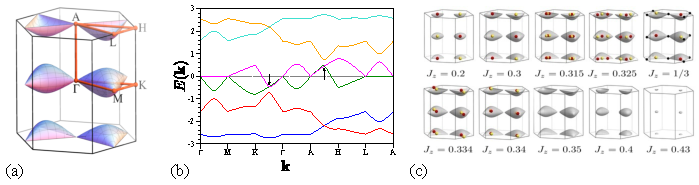
\includegraphics[width=\linewidth]{./chapter05/8_3aDispersion.pdf}
	\caption{
		(a) Brillouin zone of lattice (8,3)a with Majorana Fermi surfaces and high-symmetry points.
		(b) Majorana dispersion along high-symmetry paths
		The topological degeneracies are indicated at the band crossings between the green and pink bands between $K$ and $\Gamma$ as well as between $A$ and $H$.
		(c) Evolution of topological degeneracies and Fermi surfaces for varying exchange couplings $0.2 \leq J_z \leq 0.43$ and $J_x = J_y = (1 - J_z)/2$.
	}
	\label{fig:chapter05_8_3aDispersion}
\end{figure}
%


%
%
% LATTICE (8,3)B %%%%%%%%%%%%%%%%%%%%%%%%%%%%%%%%%%%%%%%%%%%%%%%%%%%%%%%%%%%%%%%%%%%%%%%
\subsection{Lattice (8,3)b}
\label{section:chapter05_8_3b}
%%%%%%%%%%%%%%%%%%%%%%%%%%%%%%%%%%%%%%%%%%%%%%%%%%%%%%%%%%%%%%%%%%%%%%%%%%%%%%%%%%%%%%%%
%
%
\subsubsection{Lattice information}
%
%
As mentioned in the previous section, lattice (8,3)b (subsequently referred to in the literature as the hyperhexagon lattice~\cite{SmithPRB2016,HalaszPRL2017,MasahikoPRL2018}) has a similar structure to lattice (8,3)a.
It may also be viewed as consisting of coupled triangular spirals, however, in contrast to (8,3)a, neighboring spirals rotate in opposite directions, leading to an inversion symmetric lattice (see Figure~\ref{fig:chapter05_8_3abComparison}).

Formally, lattice (8,3)b is specified by the trigonal space group $R\bar{3}m$ (No. 166) with $c/a = \sqrt{6}/5$ and Wyckoff positions for the (hexagonal) unit cell are $18(f)$ with $x=2/5$.
The concrete choice of six site unit cell used in this work is given by the site positions
%
\begin{equation}
	\begin{matrix*}[l]
		\br_1 = \left(\frac{1}{10}, \frac{1}{2\sqrt{3}}, \frac{1}{5}\sqrt{\frac{2}{3}}\right) &
		\br_2 = \left(\frac{1}{5}, \frac{\sqrt{3}}{5}, \frac{\sqrt{6}}{5}\right) &
		\br_3 = \left(\frac{3}{10}, \frac{11}{10\sqrt{3}}, \frac{4}{5}\sqrt{\frac{2}{3}}\right) \\
		&\\
		\br_4 = \left(\frac{1}{5}, \frac{2}{5\sqrt{3}}, \frac{2}{5}\sqrt{\frac{2}{3}}\right) &
		\br_5 = \left(\frac{3}{10}, \frac{3\sqrt{3}}{10}, \frac{\sqrt{6}}{5}\right) &
		\br_6 = \left(\frac{2}{5}, \frac{1}{\sqrt{3}}, \sqrt{\frac{2}{3}}\right).
	\end{matrix*}
\end{equation}
%
The lattice vectors are chosen to be
%
\begin{equation}
	\begin{matrix*}[l]
		\ba_1 = \left(\frac{1}{2}, \frac{1}{2\sqrt{3}}, \frac{1}{5}\sqrt{\frac{2}{3}}\right) \quad
		\ba_2 = \left(0, \frac{1}{\sqrt{3}}, \frac{2}{5}\sqrt{\frac{2}{3}}\right) \quad
		\ba_3 = \left(0, 0, \frac{\sqrt{6}}{5}\right)
	\end{matrix*}
\end{equation}
%
with the corresponding reciprocal lattice vectors
%
\begin{equation}
	\begin{matrix*}[l]
		\bq_1 = \left(4\pi, 0, 0\right) \quad
		\bq_2 = \left(-2\pi, 2\sqrt{3}\pi, 0\right) \quad
		\bq_3 = \left(0, -\frac{4\pi}{\sqrt{3}}, 5\sqrt{\frac{2}{3}}\pi\right).
	\end{matrix*}
\end{equation}
%

The unit cell and translation vectors are illustrated in Figure~\ref{fig:chapter05_8_3bPanel}~(a).
The bonds in the figure are colored red, green and blue to indicate the assignment of $x$-, $y$- and $z$-type bonds, respectively.
This assignment of bonds is chosen to respect as many of the lattice symmetries as possible and is unique up to an overall permutation of the three bond types.
More specifically, there are two distinct sets of $x$-, $y$- and $z$-bonds which cannot be related by symmetries, namely, those which make up the counter-rotating spirals and those which connect them.
All bonds in a given set, however, are related by a combination of a $C_3$ rotation and inversion symmetry.
The symmetry between $x$-, $y$- and $z$-bonds is reflected in the ground state phase diagram shown in Figure~\ref{fig:chapter05_8_3bPanel}~(b).
%
\begin{figure}[tb]
	\centering
	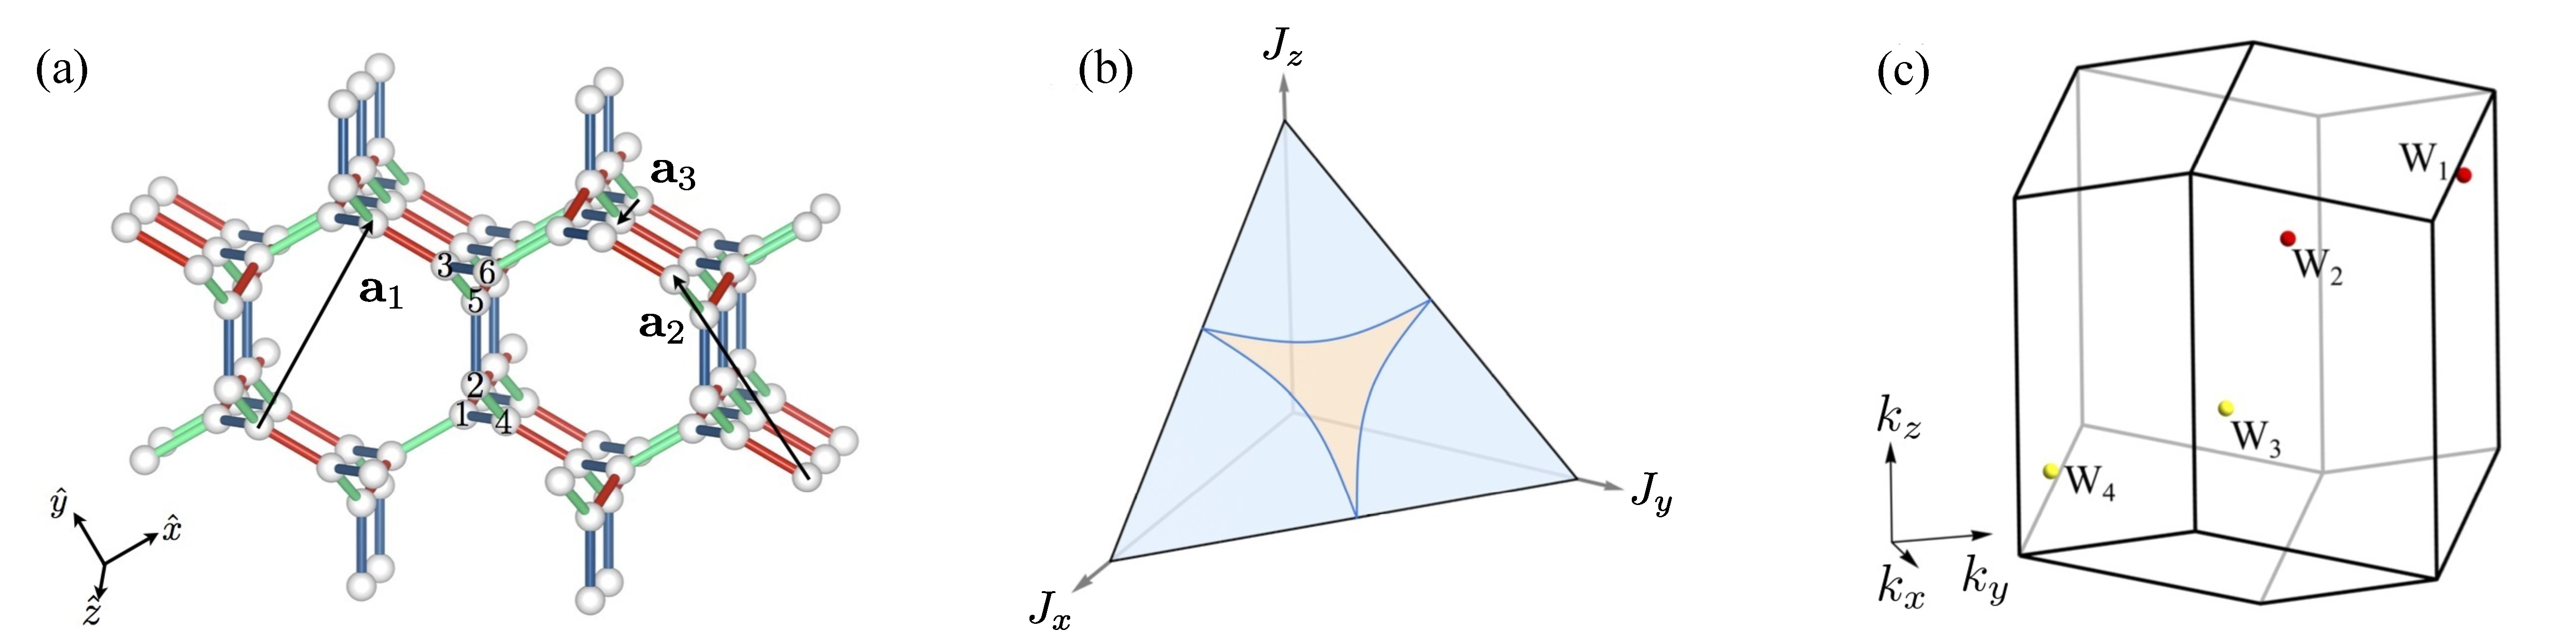
\includegraphics[width=\linewidth]{./chapter05/8_3bPanel.pdf}
	\caption{
		(a) Unit cell and translation vectors for the Kitaev model on lattice (8,3)b.
		(b) Ground state phase diagram for lattice (8,3)b.
		The regions orange shaded region corresponds to the gapless Weyl spin liquid phase.
		The blue shaded regions are gapped.
		(c) Visualization of the four Weyl nodes for isotropic exchange couplings.
		Weyl nodes of positive and negative chirality are denoted by red and yellow, respectively.
		Note that the Weyl nodes all lie on a $C_3$-invariant axis which does not pass through the origin due to its projective representation inducing a shift in momentum space.
	}
	\label{fig:chapter05_8_3bPanel}
\end{figure}
%


%
%
\subsubsection{Gauge structure}
%
%
Lattice (8,3)b possesses three loop operators of length 8 and one of length 12 per unit cell.
These four loop operators may be combined to form a closed volume leading to only \textit{three} independent loop operators per unit cell (see Appendix~\ref{appendix:ThreeDimensionalKitaevModels_8_3b} for details).
The canonical flux sector for lattice (8,3)b corresponds to $\pi$-flux through all elementary loops.
This results in all loop operators $\op{W}_p$ having eigenvalue +1.
Additionally, it has been checked numerically that the canonical flux sector is, indeed, the ground state flux sector.
The vison gap $\Delta \sim 0.16$ for lattice (8,3)b is the largest found for the lattices considered here (see Figure~\ref{fig:chapter05_VisonGaps} and Table~\ref{table:chapter05_VisonGaps}).
The vison gap has been computed by flipping the value of $u_{jk}$ for a single $z$-bond, resulting in the excitation of four loop operators (further details are given in Appendix~\ref{appendix:ThreeDimensionalKitaevModels_8_3b}).


%
%
\subsubsection{Projective symmetries}
%
%
Lattice (8,3)b is bipartite with different sublattices connected by the vectors $\br_0 = \ba_1$ and $\br'_0 = \ba_3$.
As a result, the projective representation of time-reversal is given by
%
\begin{equation}
	H(\bk) = G\dag_{\mathcal{T}}~H(-\bk + \bk_0) G_{\mathcal{T}},
\end{equation}
%
where $\bk_0 = (\bq_1 + \bq_3)/2$ and the associated gauge transformation matrix is given by
%
\begin{equation}
	G_{\mathcal{T}} =
		\begin{pmatrix}
			\id & 0 \\
			0	& -\id
		\end{pmatrix}.
\end{equation}
%
Furthermore, the lattice is inversion symmetric with projective representation
%
\begin{equation}
	H(\bk) = G\dag_{\mathcal{P}}~U_{\mathcal{P}}~H(-\bk)~U\dag_{\mathcal{P}}~G_{\mathcal{P}},
\end{equation}
%
where $U_{\mathcal{P}}$ is the matrix representation of the inversion operator acting on the unit cell indices, and the associated gauge transformation matrix $G_{\mathcal{P}}$ is identical to $G_{\mathcal{T}}$ for the gauge \textit{Ansatz} used here.
Note, however, that the gauge transformation $\op{G}_{\mathcal{P}}$ associated to the inversion operator does \textit{not} oscillate sign as a function of unit cell position $\br$ and, thus, yields a projective inversion operator that relates states at $\bk$ to states at $-\bk$.
The resulting energy relations are given by
%
\begin{equation}
	E_{\alpha}(\bk) = -E_{\beta}(-\bk) \qquad E_{\alpha}(\bk) = E_{\gamma}(-\bk + \bk_0) \qquad E_{\alpha}(\bk) = E_{\delta}(-\bk),
\end{equation}
%
due to particle-hole, time-reversal and inversion symmetry, respectively.
Due to the fact that the gauge transformation $\op{G}_{\mathcal{T}}$ relates states at momentum $\bk$ to states at momentum $\bk - \bk_0$, the momentum space Hamiltonian matrix has the form of a generic band Hamiltonian
%
\begin{equation}
	H(\bk) = 
		\begin{pmatrix}
			0			&			& A(\bk) 	\\
			& \ddots 	& 			\\
			A\dag(\bk)	&			& 0
		\end{pmatrix}
	\label{eq:chapter05_8_3bGenericHamiltonian}
\end{equation}
%
similar to lattice (8,3)a, however, with the additional property that it is inversion symmetric.


%
\subsubsection{Majorana band structure}
%
The presence of a trivially implemented projective inversion symmetry, \ie, with $\til{\bk}_0 = \bm{0}$, prohibits the formation of stable Fermi surfaces.
This can be seen by noting that the combination of particle-hole and inversion symmetries yields the relation $E_{\alpha}(\bk) = - E_{\beta}(\bk)$, preventing an isolated band from crossing the Fermi energy.
Furthermore, a doubly degenerate two-dimensional Fermi surface, while allowed by symmetry, is purely accidental and may be gapped by simply tuning the exchange couplings.

The spectrum may, however, contain the type of topological degeneracies discussed in Section~\ref{section:chapter05_8_3a}.
In this case, the degenerate bands $E_{\pm}(\bk)$ are described locally by
%
\begin{equation}
	E_{\pm}(\bk) \approx E_0(\bk^*) \pm \sum_i~b^i |k_i - k^*_i| \qquad {\rm where } \qquad b^i \in \mathbb{R}_{+}.
\end{equation}
%
Note that non-zero $E_0(\bk^*)$ may yield two-dimensional Fermi surfaces, but, as mentioned above, such Fermi surfaces are unstable.
In the case that $E_0(\bk^*) = 0$, however, these degeneracies remain pinned to zero-energy by the combination of inversion and particle-hole symmetries.

Such a degeneracy is described locally by the effective two-band Hamiltonian
%
\begin{equation}
	H_{\rm Weyl}(\bk) = \sum_{j=1}^{3}~ \bm{v}_j \cdot (\bk - \bk^*)~\tau^j,
	\label{eq:chapter05_WeylHamiltonian}
\end{equation}
%
where $\bk^*$ is the location of the degeneracy, the Fermi velocities $\bm{v}_j \in \mathbb{R}^3\backslash\{\bm{0}\}$ are linearly-independent, and $\tau^j$ are Pauli matrices acting on the degenerate bands.
This Hamiltonian may be recognized as the Weyl Hamiltonian (with anisotropic speed of light) of high-energy theory which describes massless, chiral fermions.
As such, these zero-energy degeneracies are referred to as \textit{Weyl nodes}.
Each Weyl node has a topological charge associated to its chirality which may be calculated as $\signum{[\bm{v}_1 \cdot (\bm{v}_2 \times \bm{v}_3)]}$.
More physically, Weyl nodes may be identified as monopoles of the Berry flux, where the charge of the monopole is equal to the chirality of the Weyl node.
%
\begin{figure}[tb]
	\centering
	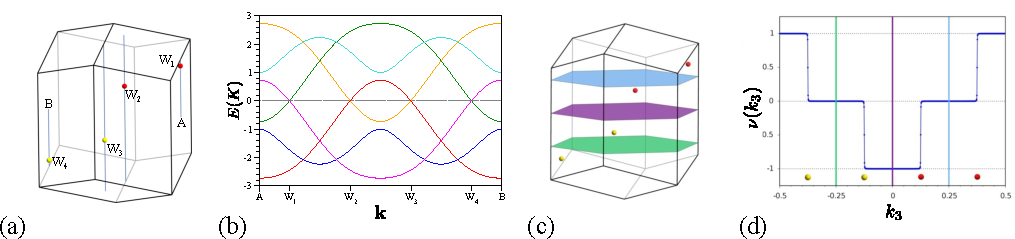
\includegraphics[width=\linewidth]{./chapter05/8_3bPanel2.pdf}
	\caption{
		(a) The Weyl nodes of lattice (8,3)b are located on the $C_3$-invariant axis, marked in blue.
		(b) Majorana dispersion plotted along the $C_3$-axis.
		(c) Brillouin zone with positions of the Weyl nodes and three example planes for which the Chern number may be calculated
		(d) Chern number $\nu(k_3)$ plotted as a function of $k_3$.
		The positions of the Weyl nodes and three example planes  ($k_3 = 0, \pm 1/4$) are indicated as a guide to the eye.
	}
	\label{fig:chapter05_8_3bPanel2}
\end{figure}
%

The form of Eq.~\eqref{eq:chapter05_WeylHamiltonian} implies that the particle-hole transformation inherent to the Kitaev spin liquids requires the presence of Weyl nodes of opposite chirality at opposite momenta $\bk^*$ and $-\bk^*$.
Similarly, the presence of inversion symmetry would imply the existence of Weyl nodes of opposite chirality at momenta $\bk^*$ and $-\bk^* + \til{\bk}_0$.
Furthermore, the presence of time-reversal symmetry would imply Weyl nodes of the \textit{same} chirality at momenta $\bk^*$ and $-\bk^* + \bk_0$.
Note that in a normal fermionic system, the presence of \textit{both} inversion and time-reversal symmetries does not allow for stable Weyl nodes, as the symmetries act to map Weyl nodes of opposite chirality onto one another.
However, the fact that the symmetries must be represented \textit{projectively} in the fermionic sector of the Kitaev spin liquid allows for the unique possibility of having a stable \textit{Weyl spin liquid} phase where both inversion and time-reversal symmetries are present.

Diagonalizing the concrete Kitaev Hamiltonian for lattice (8,3)b reveals an extended gapless Weyl spin liquid phase around the point of isotropic exchange couplings (see phase diagram in Figure~\ref{fig:chapter05_8_3bPanel}~(b)).
Due to the periodicity of the Brillouin zone, the overall Berry charge must vanish and, thus, Weyl nodes always appear in pairs of opposite chirality.
From the above discussion, it is clear that for lattice (8,3)b there must be at least four Weyl nodes due to the presence of particle-hole symmetry along with inversion symmetry (with $\til{\bk}_0 = 0$) and time-reversal symmetry.
For isotropic couplings, there are four Weyl nodes which all lie on a $C_3$-invariant axis (see Figure~\ref{fig:chapter05_8_3bPanel}~(c) or Figure~\ref{fig:chapter05_8_3bPanel2}~(a) and (b)).
Two Weyl nodes of positive charge are located at $W_1 = (5/8)\bq_1 + (3/4)\bq_2 + (3/8)\bq_3$ and $W_2 = -W_2 + \bk_0$, whereas there are two negatively charged Weyl nodes located at $W_3 = -W_2$ and $W_4 = -W_1$.

The charge of a Weyl node can be measured by computing the Chern number on an arbitrary surface which encloses it.
Due to the periodicity of the Brillouin zone, such a closed surface may be deformed into a pair of planes lying on either side of the Weyl node (refer to Figure~\ref{fig:chapter05_8_3bPanel2}~(c)).
Reversing the orientation of \textit{one} of the planes, such that both planes now have the same orientation, reverses the Chern number of that plane.
The result is that the Chern number of the original closed surface, \ie, the chirality of the Weyl node, is given by the \textit{difference} in Chern numbers between the two planes.
The Chern number for the Kitaev Hamiltonian on lattice (8,3)b with isotropic couplings is plotted as a function of $k_3 = \bk \cdot \bq_3 / 2\pi$ in Figure~\ref{fig:chapter05_8_3bPanel2}~(d), \ie, each plane has a fixed value of $k_3$.
One may see that at $k_3$-values corresponding to a plane containing a Weyl node, the Chern number jumps by the respective charge of that Weyl node.

Figure~\ref{fig:chapter05_8_3bWeyl1}~(a) shows the evolution of the Weyl nodes in the 3D Brillouin zone as the exchange couplings are varied for $0 \leq J_z \lesssim 0.43$ with $J_x = J_y = (1 - J_z)/2$.
The trajectory of negatively charged Weyl nodes changes colors from yellow to green as $J_z$ is increased, whereas the trajectory of positively charged Weyl nodes changes from red to green.
As $J_z$ is increased, Weyl nodes of opposite chirality move towards each other, ultimately meeting and mutually annihilating at the $\Gamma$-point and at $\bk_0$ for $J_z \approx 0.43$.
For decreasing $J_z$, the Weyl nodes similarly move through the Brillouin zone, however, rather than meeting and mutually annihilating at isolated momenta, the velocity vectors of the isolated Weyl nodes vanish, collapsing the bulk gap.
Note that, away from the isotropic point the $C_3$-symmetry is broken and, thus, the Weyl nodes are free to leave the $C_3$-invariant axis.
%
\begin{figure}[tb]
	\centering
	
\includegraphics[width=\linewidth]{./chapter05/8_3bWeyl1.pdf}
	\caption{
		(a) Evolution of Weyl nodes of lattice (8,3)b for varied coupling constants $0 \leq J_z \lesssim 0.43$ with $J_x = J_y = (1 - J_z)/2$.
		(b) Corresponding Fermi arc evolution.
		(c) Visualization of the surface Brillouin zone for the 001-surface.
	}
	\label{fig:chapter05_8_3bWeyl1}
\end{figure}
%

Figure~\ref{fig:chapter05_8_3bWeyl1}~(b) shows the associated Fermi arc surface states for the 001-surface Brillouin zone of a slab geometry.
The surface Brillouin zone is visualized in Figure~\ref{fig:chapter05_8_3bWeyl1}~(c).
Fermi arcs are exact zero-energy surface states which connect Weyl nodes of opposite chirality (more accurately, their projections to the surface Brillouin zone).
The Fermi arcs inherit a topological protection from their associated Weyl nodes -- as long as the Weyl nodes are left intact, no perturbation can gap their surface states.
As the Weyl nodes wander through the bulk Brillouin zone, the Fermi arcs are seen to deform, ultimately shrinking to nothing as the Weyl nodes meet and annihilate for $J_z \approx 0.43$.

Breaking time-reversal symmetry by applying an external magnetic field also causes the Weyl nodes to wander around the Brillouin zone as seen in Figure~\ref{fig:chapter05_8_3bWeyl2}~(a) for $0 \leq \kappa \leq 0.25$.
At $\kappa \approx 0.2$, two Weyl nodes of opposite chirality meet and mutually annihilate at a high-symmetry point in the Brillouin zone.
Note that, since application of a magnetic field in the 111-direction does not break $C_3$-symmetry, the Weyl nodes are pinned to the $C_3$-invariant axis.
In Figure~\ref{fig:chapter05_8_3bWeyl2}~(b) are pictured the corresponding Fermi arcs in the 001-surface Brillouin zone.
As $\kappa$ is tuned from 0 to 0.2, the Fermi arcs become increasingly warped as two Weyl nodes of opposite chirality move towards each other.
As $\kappa$ is increased further, the two Fermi arcs meet at a high-symmetry point, becoming a single Fermi arc.
For still larger values of $\kappa$, even more Weyl nodes begin to appear in charge-neutral pairs while other pairs mutually annihilate.
%
\begin{figure}[tb]
	\centering
	
\includegraphics[width=\linewidth]{./chapter05/8_3bWeyl2.pdf}
	\caption{
		(a) Evolution of Weyl nodes of lattice (8,3)b in the presence of a magnetic field of varied strength $0 \leq \kappa \leq 0.25$.
		(b) Corresponding Fermi arc evolution.
		(c) Visualization of the surface Brillouin zone for the 001-surface.
	}
	\label{fig:chapter05_8_3bWeyl2}
\end{figure}
%


%
%
% LATTICE (8,3)C %%%%%%%%%%%%%%%%%%%%%%%%%%%%%%%%%%%%%%%%%%%%%%%%%%%%%%%%%%%%%%%%%%%%%%%
\subsection{Lattice (8,3)c}
\label{section:chapter05_8_3c}
%%%%%%%%%%%%%%%%%%%%%%%%%%%%%%%%%%%%%%%%%%%%%%%%%%%%%%%%%%%%%%%%%%%%%%%%%%%%%%%%%%%%%%%%
%
%
\subsubsection{Lattice information}
%
%
Lattice (8,3)c can be viewed as parallel zigzag chains which run along the $z$-direction and which are coupled by vertices lying in the $x-y$ plane.
Formally, lattice (8,3)c is specified by the hexagonal space group $P6_{3}/mmc$ (No. 194) with $c/a = 2/5$ and Wyckoff positions for the unit cell are $2(c)$ and $6(h)$ with $x=7/15$.
The concrete choice of eight site unit cell used in this work is given by the site positions
%
\begin{equation}
	\begin{matrix*}[l]
		\br_1 = \left(-\frac{1}{5}, \frac{4}{5\sqrt{3}}, \frac{1}{10}\right) &
		\br_2 = \left(0, \frac{7}{5\sqrt{3}}, \frac{1}{10}\right) &
		\br_3 = \left(\frac{1}{5}, \frac{4}{5\sqrt{3}}, \frac{1}{10}\right) \\
		&\\
		\br_4 = \left(\frac{1}{2}, \frac{1}{2\sqrt{3}}, \frac{3}{10}\right) &
		\br_5 = \left(0, \frac{1}{\sqrt{3}}, \frac{1}{10}\right) &
		\br_6 = \left(\frac{3}{10}, \frac{7}{10\sqrt{3}}, \frac{3}{10}\right) \\
		&\\
		\br_7 = \left(\frac{1}{2}, \frac{1}{10\sqrt{3}}, \frac{3}{10}\right) &
		\br_8 = \left(\frac{7}{10}, \frac{7}{10\sqrt{3}}, \frac{3}{10}\right).
	\end{matrix*}
\end{equation}
%
The lattice vectors are chosen to be
%
\begin{equation}
	\begin{matrix*}[l]
		\ba_1 = \left(1, 0, 0\right) \qquad
		\ba_2 = \left(-\frac{1}{2}, \frac{\sqrt{3}}{2}, 0\right) \qquad
		\ba_3 = \left(0, 0, \frac{2}{5}\right)
	\end{matrix*}
\end{equation}
%
with the corresponding reciprocal lattice vectors
%

%
\begin{equation}
	\begin{matrix*}[l]
		\bq_1 = \left(2\pi, \frac{2\pi}{\sqrt{3}}, 0\right) \qquad
		\bq_2 = \left(0, \frac{4\pi}{\sqrt{3}}, 0\right) \qquad
		\bq_3 = \left(0, 0, 5\pi\right).
	\end{matrix*}
\end{equation}
%

The unit cell and translation vectors are illustrated in Figure~\ref{fig:chapter05_8_3cPanel}~(a).
The bonds in the figure are colored red, green and blue to indicate the assignment of $x$-, $y$- and $z$-type bonds, respectively.
When choosing the assignment of bonds for this lattice, one finds that for each of the chains there are two inequivalent choices.
The assignment of bonds used here is chosen to respect as many of the lattice symmetries as possible. 
More specifically, there are two distinct sets of $x$-, $y$- and $z$-bonds, namely those forming the zigzag chains along the z-direction and those lying in the $x-y$ plane.
The set of all $x$-, $y$- and $z$-bonds are related to each other by a sixfold screw axis.
The symmetry between $x$-, $y$- and $z$-bonds is reflected in the phase diagram shown in Figure~\ref{fig:chapter05_8_3cPanel}~(b).
%
\begin{figure}[tb]
	\centering
	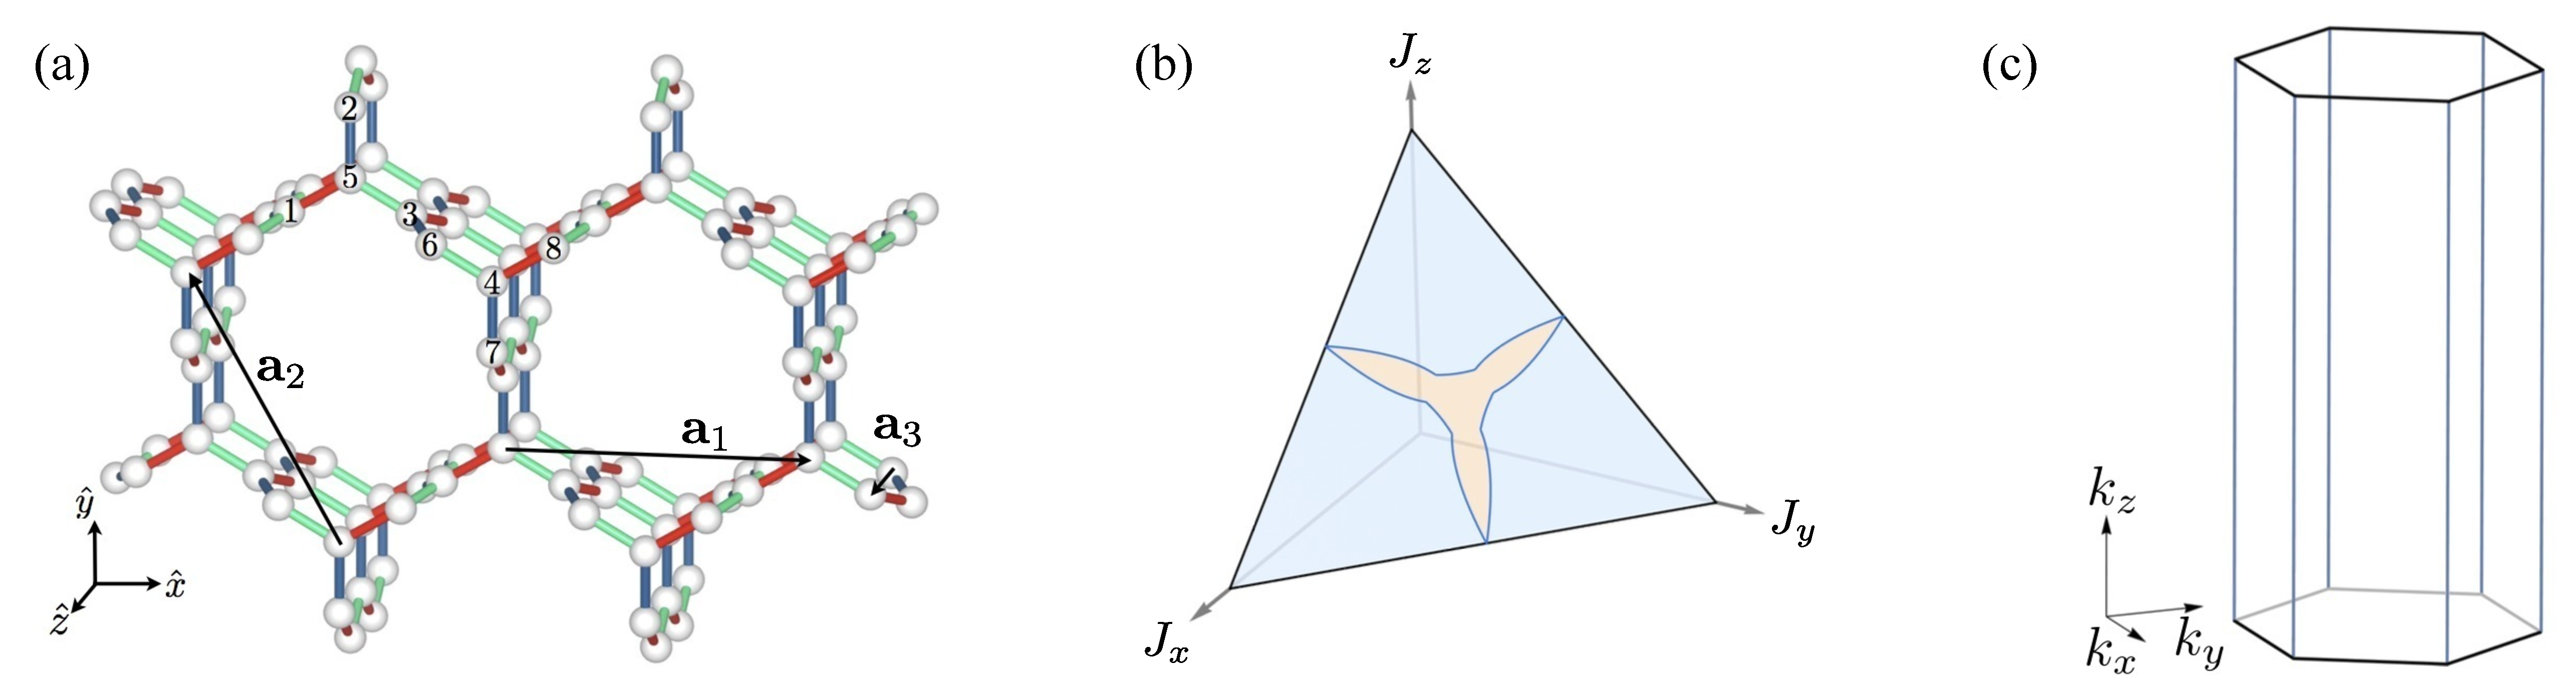
\includegraphics[width=\linewidth]{./chapter05/8_3cPanel.pdf}
	\caption{
		(a) Unit cell and translation vectors for the Kitaev model on lattice (8,3)c.
		(b) Phase diagram for lattice (8,3)c.
		The orange shaded regions correspond to a gapless phase with line nodes.
		The blue shaded regions are gapped.
		(c) The line nodes (marked in blue) are located precisely at the edges of the Brillouin zone for isotropic exchange couplings.
	}
	\label{fig:chapter05_8_3cPanel}
\end{figure}
%


%
%
\subsubsection{Gauge structure}
%
%
Lattice (8,3)c possesses six loop operators of length 8 and one of length 18 per unit cell.
These seven loop operators may be combined to form three closed volumes leading to only \textit{four} independent loop operators per unit cell (see Appendix~\ref{appendix:ThreeDimensionalKitaevModels_8_3c} for details).
The canonical flux sector for lattice (8,3)c corresponds to $\pi$-flux through all loops of length 8 and $0$-flux through all loops of length 18.

It turns out, however, that it is not possible to achieve the canonical flux sector for lattice (8,3)c.
As it takes three loops of length 8 to form a closed volume which is constrained to have vanishing total flux, one may assign $\pi$-flux either to only two of the loops or to none of the loops.
Lieb's theorem indicates that the system would prefer to thread $\pi$-flux through as many plaquettes as possible and, thus, the former option leads to lower energy.
Unfortunately, it is not \textit{a priori} clear which of the plaquettes should be assigned $0$-flux.

For highly anisotropic couplings, \eg, $J_z \gg J_x = J_y$, there exists a unique ground state flux configuration corresponding to a threading of $\pi$-flux through the loops which contain three $z$-bonds and $0$-flux through the two remaining loops which contain only two $z$-bonds, a result which is derived in Appendix~\ref{appendix:LoopModels_8_3c}.
This perturbative result was later confirmed by a subsequent quantum Monte Carlo study~\cite{EschmannPRL2019} of the Kitaev model on lattice (8,3)c.
Additionally, this study suggests that at the isotropic point, there is a sub-extensive degeneracy of ground states with columnar flux order.
Away from the isotropic point, where $C_3$ symmetry is broken explicitly, however, the system uniquely selects one of these ground states.

The work presented in this chapter, however, does not tackle the problem of finding the actual ground state flux configuration of the system.
Instead, the flux sector corresponding to all plaquettes having $0$-flux is used to illustrate the ideas of the classification scheme.
This flux sector is the only one which respects all of the lattice symmetries, but is not frustrated.
Such a flux sector can always be stabilized as the ground state by adding terms to the Hamiltonian which penalize $\pi$-flux through plaquettes, similar to what was done in Reference~\cite{LaiPRB2011} for the Kitaev model on the two-dimensional square-octagon lattice.
Note that the results reported below are, indeed, qualitatively correct~\cite{EschmannPRL2019} also for the true ground state spin liquid on lattice (8,3)c.
The vison gap for lattice (8,3)c is not reported here as calculations were not done in the ground state sector, however, it is worth noting that an elementary vison excitation results in the excitation of four loop operators (further details are given in Appendix~\ref{appendix:ThreeDimensionalKitaevModels_8_3c}).


%
%
\subsubsection{Projective symmetries}
%
%
Lattice (8,3)c is bipartite with sublattices having the same translation symmetry as the elementary unit cell.
The resulting projective representation of time-reversal is given by
%
\begin{equation}
	H(\bk) = G\dag_{\mathcal{T}}~H(-\bk)~G_{\mathcal{T}},
\end{equation}
%
where the associated gauge transformation matrix is given by
%
\begin{equation}
	G_{\mathcal{T}} =
		\begin{pmatrix}
			\id & 0 \\
			0	& -\id
		\end{pmatrix}.
\end{equation}
%
Furthermore, the lattice is inversion symmetric with projective representation
%
\begin{equation}
	H(\bk) = G\dag_{\mathcal{P}}~U_{\mathcal{P}}~H(-\bk)~U\dag_{\mathcal{P}}~G_{\mathcal{P}},
\end{equation}
%
where $U_{\mathcal{P}}$ is the matrix representation of the inversion operator acting on the unit cell, and the associated gauge transformation matrix $G_{\mathcal{P}}$ is identical to $G_{\mathcal{T}}$ for the gauge \textit{Ansatz} used here.
The resulting energy relations are given by
%
\begin{equation}
	E_{\alpha}(\bk) = -E_{\beta}(-\bk) \qquad {\rm and } \qquad E_{\alpha}(\bk) = E_{\gamma}(-\bk),
\end{equation}
%
where the first relation is due to particle-hole symmetry and the second is enforced individually by both time-reversal and inversion symmetry.
Due to the fact that the gauge transformation $\op{G}_{\mathcal{T}}$ is constant as a function of unit cell position,
the momentum space Hamiltonian matrix has the block off-diagonal form
%
\begin{equation}
	H(\bk) =
		\begin{pmatrix}
			0			& A(\bk) \\
			A\dag(\bk)	& 0
		\end{pmatrix}.
		\label{eq:chapter05_8_3cGenericHamiltonian}
\end{equation}
%


%
%
\subsubsection{Majorana band structure}
%
%
As was the case for lattice (8,3)b, a trivially implemented projective inversion symmetry prevents the formation of stable Fermi surfaces.
Unlike lattice (8,3)b, however, the projective time-reversal operator is also implemented trivially, yielding a block off-diagonal Hamiltonian matrix as in Eq.~\eqref{eq:chapter05_8_3cGenericHamiltonian}.
Zero modes at a given momentum correspond to vanishing of the determinant of $H(\bk)$, which, in this case, means the simultaneous vanishing of $\Re{(\det{A(\bk)})}$ and $\Im{(\det{A(\bk)})}$.
In three-dimensions, solutions to the above correspond to a one-dimensional manifold of $\bk$-points.
The conclusion is that for the Kitaev model defined on lattice (8,3)c, the only stable zero-energy manifolds are \textit{nodal lines}.

In fact, such nodal lines are protected by the presence of time-reversal symmetry and may be characterized by an integer invariant~\cite{BurkovPRB2011,ZhaoPRL2013,MatsuuraNJP2013}
%
\begin{equation}
	\nu = -\frac{1}{2\pi} \Im{\oint_S}~dt~\trace{[\partial_t \log A(\bk)]},
\end{equation}
%
where $S$ is a closed path in momentum space parameterized by $t$, and $\nu$ is seen to be the winding number of the map $\bk \in S \mapsto A(\bk)$.
For loops $S$ which are pierced by the nodal line, this winding number is non-zero.
As this integer winding number cannot be changed continuously, it represents an obstruction to gapping out the nodal line.
Thus, without breaking time-reversal symmetry, this can only be done by shrinking the nodal line to a point.
If time-reversal symmetry is broken, however, the winding number is no longer well-defined and such a nodal line becomes unstable.

Diagonalizing the concrete Kitaev Hamiltonian for lattice (8,3)c reveals an extended gapless phase around the point of isotropic exchange couplings (see Figure~\ref{fig:chapter05_8_3cPanel}~(b)), where the zero modes correspond to nodal lines located at $(\pm\frac{4\pi}{3}, 0, k_z)$ as pictured in Figure~\ref{fig:chapter05_8_3cPanel}~(c).
Also visible in the Figure is a surface of gapless modes at the top (bottom) of the Brillouin zone.
As discussed above, this surface cannot be stable and, in fact, gaps out as soon as the couplings are tuned away from the isotropic point.

As mentioned above, the nodal line is protected by the presence of time-reversal symmetry.
Introducing an infinitesimal external magnetic field immediately gaps the nodal line almost entirely.
However, adding a magnetic field term to the model does not break the inversion symmetry of lattice (8,3)c.
As a result, for fixed $\bk$, the Hamiltonian is of the same form as that discussed for lattice (8,3)b, where time-reversal symmetry was present, albeit with a shift in momentum space.
As a result, the nodal line is gapped with the exception of six isolated points corresponding to stable Weyl nodes.
A similar situation was studied in Reference~\cite{HermannsPRL2015} for lattice (10,3)b and is discussed in Section~\ref{section:chapter05_10_3b}.
%
\begin{figure}[tb]
	\centering
	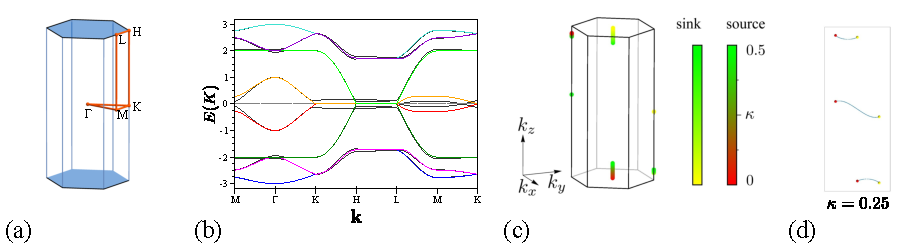
\includegraphics[width=\linewidth]{./chapter05/8_3cPanel2.pdf}
	\caption{
		(a) Brillouin zone of lattice (8,3)c with high-symmetry points.
		The nodal lines and surfaces are marked in blue.
		(b) Majorana dispersion plotted along the high-symmetry paths.
		(c) Evolution of the Weyl nodes in the presence of a magnetic field of varying strength $0 \leq \kappa \leq 0.5$.
		(d) Corresponding Fermi arcs for $\kappa = 0.25$.
	}
	\label{fig:chapter05_8_3cPanel2}
\end{figure}
%

The evolution of these Weyl nodes is pictured in Figure~\ref{fig:chapter05_8_3cPanel2}~(c) for varying magnetic field strengths corresponding to $0 \leq \kappa \leq 0.5$.
For this range of $\kappa$, the Weyl nodes move very little along high-symmetry lines of the Brillouin zone.
However, for larger values of $\kappa$, many Weyl nodes appear in charge-neutral pairs while other pairs mutually annihilate.
In Figure~\ref{fig:chapter05_8_3cPanel2}~(d) are pictured the corresponding Fermi arc surface states in the 100-surface Brillouin zone for $\kappa = 0.25$.


%
%
% LATTICE (8,3)N %%%%%%%%%%%%%%%%%%%%%%%%%%%%%%%%%%%%%%%%%%%%%%%%%%%%%%%%%%%%%%%%%%%%%%%
\subsection{Lattice (8,3)n}
\label{section:chapter05_8_3n}
%%%%%%%%%%%%%%%%%%%%%%%%%%%%%%%%%%%%%%%%%%%%%%%%%%%%%%%%%%%%%%%%%%%%%%%%%%%%%%%%%%%%%%%%
%
%
\subsubsection{Lattice information}
%
%
Lattice (8,3)n can be viewed as a three-dimensional generalization of the square-octagon lattice, where layers of square-octagon lattices are coupled via mid-bond sites.
Formally, lattice (8,3)n is specified by the tetragonal space group $I4/mmm$ (No. 139) with $c/a = \frac{4}{2\sqrt{3} + \sqrt{2}}$ and Wyckoff positions for the unit cell are $16(k)$ and $16(n)$ with $x = \frac{\sqrt{3} + \sqrt{2}}{2(2\sqrt{3} + \sqrt{2})}$ and $z=1/8$.
The concretely choice of unit cell used in this work has 16 sites.
In order to simplify notation, the following basis is defined:
%
\begin{equation}
	\begin{matrix*}[l]
		\ba = \left(1, 0, 0\right) \qquad
		\bb = \left(0, 1, 0\right) \qquad
		\bc = \left(0, 0, \frac{4}{2\sqrt{3} + \sqrt{2}}\right).
	\end{matrix*}
\end{equation}
%
In the basis $(\ba, \bb, \bc)$, the positions of the sites are given by\pagebreak
%
\begin{equation}
	\begin{matrix*}[l]
		\br_{1} = \left(\frac{1}{2} + x, x, \frac{1}{4} \right) &
		\br_{2} = \left(\frac{3}{2} - x, x, \frac{1}{4} \right) &
		\br_{3} = \left(\frac{3}{2} - x, 1 - x, \frac{1}{4} \right) \\
		&\\
		\br_{4} = \left(\frac{1}{2} + x, 1 - x, \frac{1}{4} \right) &
		\br_{5} = \left(1, x, -z \right) &
		\br_{6} = \left(\frac{3}{2} - x, \frac{1}{2}, -\frac{1}{2} + z \right) \\
		&\\
		\br_{7} = \left(1, 1 - x, -z \right) &
		\br_{8} = \left(\frac{1}{2} + x, \frac{1}{2}, -\frac{1}{2} + z \right) &
		\br_{9} = \left(\frac{1}{2} + x, \frac{1}{2}, \frac{1}{2} - z \right) \\
		&\\
		\br_{10} = \left(1, x, z \right) &
		\br_{11} = \left(\frac{3}{2} - x, \frac{1}{2}, \frac{1}{2} - z \right) &
		\br_{12} = \left(1, 1-x, z \right) \\
		&\\
		\br_{13} = \left(\frac{1}{2} + x, x, -\frac{1}{4} \right) &
		\br_{14} = \left(\frac{3}{2} - x, x, -\frac{1}{4} \right) &
		\br_{15} = \left(\frac{3}{2} -x, 1 - x, -\frac{1}{4} \right) \\
		&\\
		\br_{16} = \left(\frac{1}{2} + x, 1 - x, -\frac{1}{4} \right),
	\end{matrix*}
\end{equation}
%
where $x = \frac{\sqrt{3} + \sqrt{2}}{2(2\sqrt{3} + \sqrt{2})}$ and $z=1/8$.
The lattice vectors are chosen to be
%
\begin{equation}
	\begin{matrix*}[l]
		\ba_1 = \ba \qquad
		\ba_2 = \bb \qquad
		\ba_3 = \frac{1}{2}(\ba + \bb + \bc)
	\end{matrix*}
\end{equation}
%
with the corresponding reciprocal lattice vectors (passing back to the standard orthonormal basis)
%
\begin{equation}
	\begin{matrix*}[l]
		\bq_1 = \left(2\pi, 0, -\sqrt{\frac{7}{2} + \sqrt{6}}\pi\right) &
		\bq_2 = \left(0, 2\pi, -\sqrt{\frac{7}{2} + \sqrt{6}}\pi\right) \\
		&\\
		\bq_3 = \left(0, 0, 2\sqrt{\frac{7}{2} + \sqrt{6}}\pi\right). &
	\end{matrix*}
\end{equation}
%

The unit cell and translation vectors are illustrated in Figure~\ref{fig:chapter05_8_3nPanel}~(a).
The bonds in the figure are colored red, green and blue to indicate the assignment of $x$-, $y$- and $z$-type bonds, respectively.
This assignment of bonds is chosen to be compatible with the $C_4$ and inversion symmetries of the lattice and is unique up to an overall permutation of the bond types.
All $x$- and $y$-bonds are related by a combination of inversion, $C_4$ and mirror symmetries.
The $z$-bonds come in two distinct sets, namely, those which lie in the $x-y$ plane and connect nearest neighbor "squares" and those that lie along the $z$-direction and connect neighboring "square-octagon" planes.
All $z$-bonds contained within a given set are related to each other by $C_4$ symmetry.
However, $z$-bonds are not related to any other type of bond via lattice symmetries.
The symmetry between $x$- and $y$-bonds is reflected in the ground state phase diagram shown in Figure~\ref{fig:chapter05_8_3nPanel}~(b).
%
\begin{figure}[tb]
	\centering
	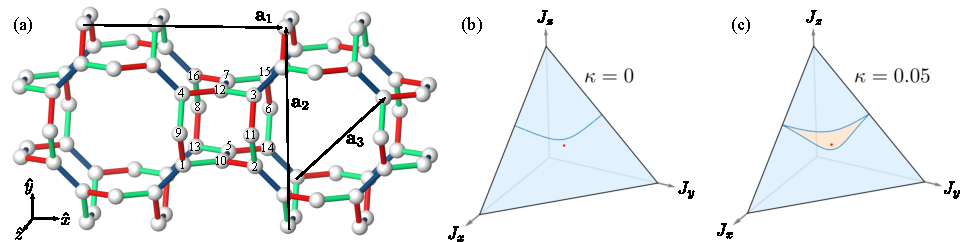
\includegraphics[width=\linewidth]{./chapter05/8_3nPanel.pdf}
	\caption{
		(a) Unit cell and translation vectors for the Kitaev model on lattice (8,3)n.
		(b) Ground state phase diagram for lattice (8,3)n.
		The Kitaev model on lattice (8,3)n has no gapless phase.
		The blue line indicates the phase transition between two distinct gapped phases.
		The isotropic point is denoted by a red dot.
		(c) Ground state phase diagram for $\kappa = 0.05$.
		For finite $\kappa$, the Dirac nodes split into pairs of oppositely charged Weyl nodes and the phase transition line evolves to a Weyl spin liquid phase, denoted by the orange shaded region.
	}
	\label{fig:chapter05_8_3nPanel}
\end{figure}
%


%
%
\subsubsection{Gauge structure}
%
%
Lattice (8,3)n possesses six loop operators of length 8, four of length 10, and two of length 12 per unit cell.
These twelve loop operators may be combined to form four closed volumes leading to only \textit{eight} independent loop operators per unit cell (see Appendix~\ref{appendix:ThreeDimensionalKitaevModels_8_3n} for details).
The canonical flux sector for lattice (8,3)n corresponds to $\pi$-flux through all loops of length 8 or 12 and $0$-flux through all loops of length 10.
This results in all loop operators $\op{W}_p$ having eigenvalue $+1$.
Additionally, it has been checked numerically that the canonical flux sector is, indeed, the ground state flux sector.
The vison gap for lattice (8,3)n shown in Figure~\ref{fig:chapter05_VisonGaps}~and Table~\ref{table:chapter05_VisonGaps}~has been computed by flipping the value of $u_{jk}$ for a single $z$-bond, resulting in the excitation of four loop operators (further details are given in Appendix~\ref{appendix:ThreeDimensionalKitaevModels_8_3n}).


%
\subsubsection{Projective symmetries}
%
%
Lattice (8,3)n is bipartite with sublattices having the same translation symmetry as the elementary unit cell.
The resulting projective representation of time-reversal is given by
%
\begin{equation}
	H(\bk) = G\dag_{\mathcal{T}}~H(-\bk)~G_{\mathcal{T}},
\end{equation}
%
where the associated gauge transformation matrix is given by
%
\begin{equation}
	G_{\mathcal{T}} =
		\begin{pmatrix}
			\id & 0 \\
			0	& -\id
		\end{pmatrix}.
\end{equation}
%
Furthermore, the lattice is inversion symmetric with projective representation
%
\begin{equation}
	H(\bk) = G\dag_{\mathcal{P}}~U_{\mathcal{P}}~H(-\bk + \til{\bk}_0)~U\dag_{\mathcal{P}}~G_{\mathcal{P}},
\end{equation}
%
where $\til{\bk}_0 = \bq_3/2$, $U_{\mathcal{P}}$ is the matrix representation of the inversion operator acting on the unit cell, and the associated gauge transformation matrix $G_{\mathcal{P}}$ is identical to $G_{\mathcal{T}}$  for the gauge \textit{Ansatz} used here.
The non-vanishing value of $\til{\bk}_0$ is due to the fact that, for a translationally invariant gauge \textit{Ansatz}, the gauge transformation $\op{G}_{\mathcal{P}}$ associated to the inversion operator oscillates sign as a function of unit cell position $\br$.
The resulting energy relations are given by
%
\begin{equation}
	E_{\alpha}(\bk) = -E_{\beta}(-\bk) \qquad E_{\alpha}(\bk) = E_{\gamma}(-\bk) \qquad E_{\alpha}(\bk) = E_{\delta}(-\bk + \til{\bk}_0),
\end{equation}
%
due to particle-hole, time-reversal and inversion symmetry, respectively.
Due to the fact that the gauge transformation $\op{G}_{\mathcal{T}}$ is constant as a function of unit cell position, the momentum space Hamiltonian matrix has the block off-diagonal form
%
\begin{equation}
	H(\bk) =
		\begin{pmatrix}
			0			& A(\bk) \\
			A\dag(\bk)	& 0
		\end{pmatrix}.
\end{equation}
%


%
%
\subsubsection{Majorana band structure}
%
%
As discussed in the context of lattice (8,3)c, due to the trivial implementation of the projective time-reversal operator, \ie, with $\bk_0 = 0$, the only stable nodal manifolds for lattice (8,3)n could be nodal lines.
In fact, what one finds upon diagonalization of the concrete Kitaev Hamiltonian, is that lattice (8,3)n turns out to be the only lattice considered in this work which does \textit{not} exhibit a gapless phase (see Figure~\ref{fig:chapter05_8_3nPanel}~(b) for the ground state phase diagram and Figure~\ref{fig:chapter05_8_3nPanel2}~(b) for the dispersion at the isotropic point).
Instead, there are two \textit{gapped} phases separated by a line of phase transitions for which the dispersion exhibits three-dimensional Dirac nodes of two doubly degenerate bands (see Figure~\ref{fig:chapter05_8_3nPanel2}~(c) and (d)).

One way of thinking of these three-dimensional Dirac nodes is as a combination of two oppositely charged Weyl nodes.
One way to split these Weyl nodes is by breaking time-reversal symmetry.
Indeed, introducing a magnet field splits the Dirac nodes into oppositely charged Weyl nodes as illustrated in Figure~\ref{fig:chapter05_8_3nPanel2}~(d).
As a result, this line of phase transitions becomes an extended gapless phase (see Figure~\ref{fig:chapter05_8_3nPanel}~(c)).
For small values of $\kappa$, this gapless phase is a Weyl spin liquid.
However, with time-reversal symmetry broken and projective inversion symmetry offering no protection, the Weyl nodes are not pinned to zero energy as is the case for lattices (8,3)b and (8,3)c above.
In fact, for sufficiently large values of $\kappa$, the degeneracies move away from zero energy, resulting in topologically protected Fermi surfaces as seen for lattice (8,3)a.
Note that the Fermi surfaces here are related by the perfect nesting vector $\til{\bk}_0$ due to the presence of inversion symmetry.
%
\begin{figure}[tb]
	\centering
	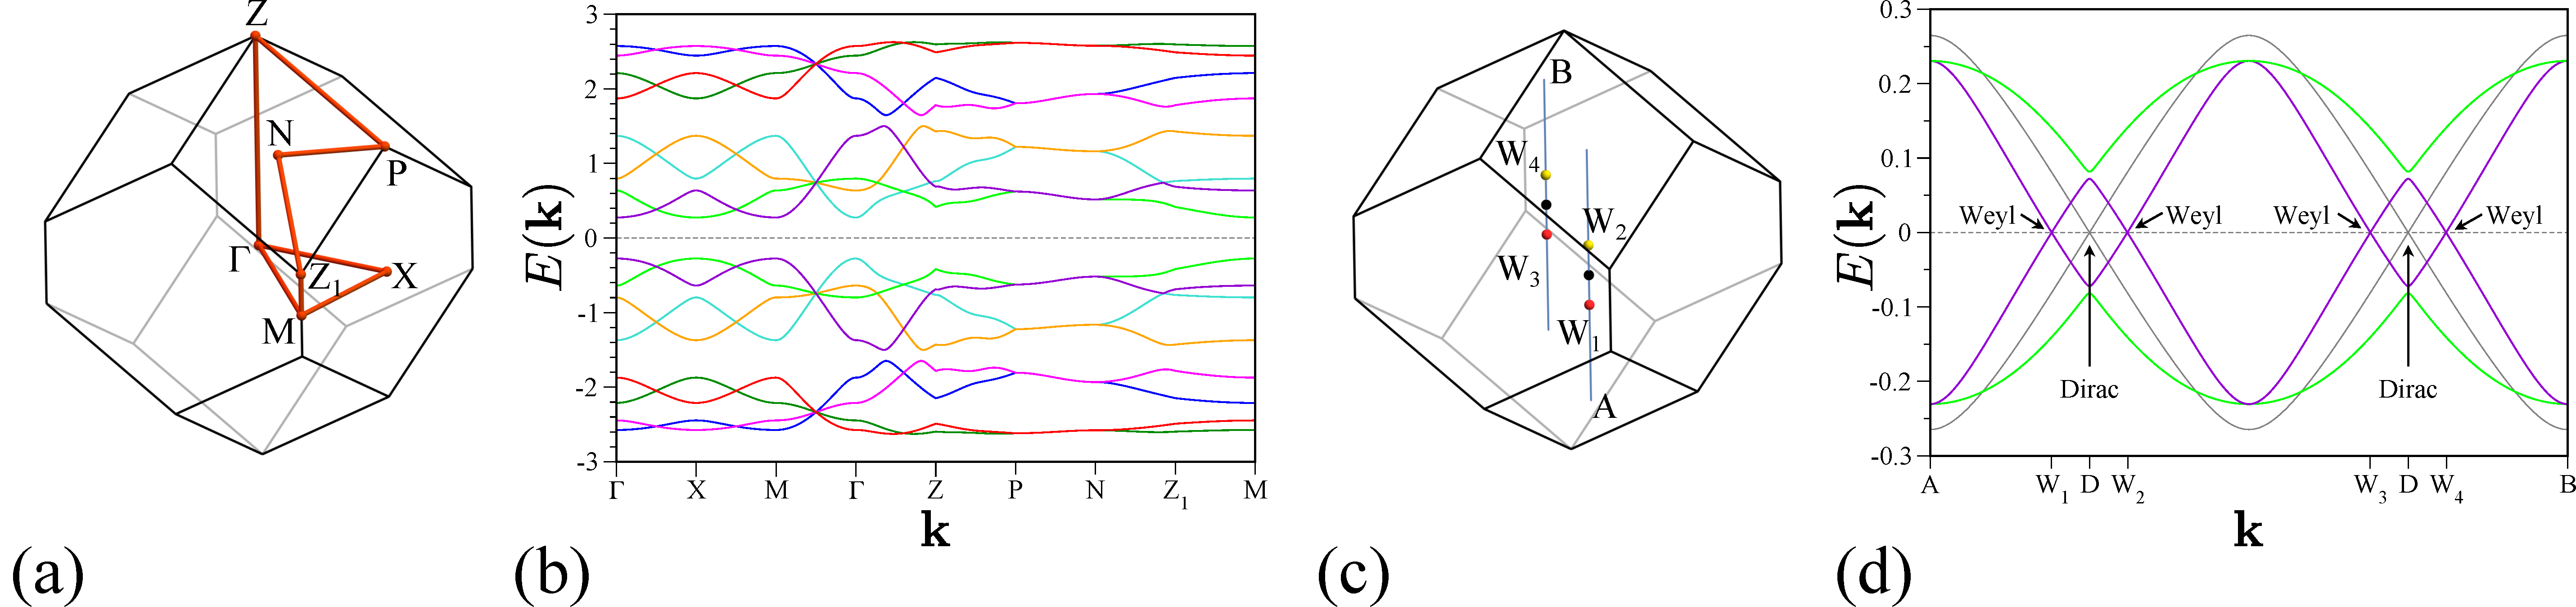
\includegraphics[width=\linewidth]{./chapter05/8_3nPanel2.pdf}
	\caption{
		(a) Brillouin zone of lattice (8,3)n with high-symmetry points.
		(b) Majorana dispersion plotted along a high-symmetry path.
		(c) Brillouin zone a path cutting through the Dirac/Weyl nodes.
		(d) Dispersion along the path in shown in (c).
		Gray lines correspond to $\kappa = 0$ while green lines correspond to $\kappa = 0.05$.
	}
	\label{fig:chapter05_8_3nPanel2}
\end{figure}
%


%
%
% LATTICE (9,3)A %%%%%%%%%%%%%%%%%%%%%%%%%%%%%%%%%%%%%%%%%%%%%%%%%%%%%%%%%%%%%%%%%%%%%%%
\subsection{Lattice (9,3)a}
\label{section:chapter05_9_3a}
%%%%%%%%%%%%%%%%%%%%%%%%%%%%%%%%%%%%%%%%%%%%%%%%%%%%%%%%%%%%%%%%%%%%%%%%%%%%%%%%%%%%%%%%
%
%
\subsubsection{Lattice information}
%
%
Lattice (9,3)a (subsequently referred to in the literature as the hypernonagon lattice~\cite{YasuyukiPRB2017,KatoPB2018,MasahikoPRL2018}) is the only non-bipartite lattice considered in this work.
Formally, lattice (8,3)a is specified by the trigonal space group $R\bar{3}m$ (No. 166) with $c/a = \frac{\sqrt{6(4 + \sqrt{3})}}{1 + 2\sqrt{3}}$ and Wyckoff positions for the unit cell are $18(f)$ with $x = \frac{\sqrt{3}}{1 + 2\sqrt{3}}$, $y = z = 0$, and $18(h)$ with $x = \frac{1 + \sqrt{3}}{4(1 + 2\sqrt{3})}$ and $z = 3/4$.
The concrete choice of unit cell used in this work has 12 sites.
In order to simplify notation, the following basis is defined:
%
\begin{equation}
	\begin{matrix*}[l]
		\ba = \left(1, 0, 0\right) \qquad
		\bb = \left(-\frac{1}{2}, \frac{\sqrt{3}}{2}, 0\right) \qquad
		\bc = \left(0, 0, \frac{\sqrt{6(4 + \sqrt{3})}}{1 + 2\sqrt{3}}\right).
	\end{matrix*}
\end{equation}
%
In the basis $(\ba, \bb, \bc)$, the positions of the sites are
%
\begin{equation}
	\begin{matrix*}[l]
		\br_{1} = \left(\delta_f, 0, 0\right) &
		\br_{2} = \left(2\delta_h, \delta_h, \frac{1}{12}\right) &
		\br_{3} = \left(\delta_f, \delta_f, 0\right) \\
		&\\
		\br_{4} = \left(\delta_h, 2\delta_h, -\frac{1}{12}\right) &
		\br_{5} = \left(0, \delta_f, 0\right) &
		\br_{6} = \left(-\delta_h, \delta_h, \frac{1}{12}\right) \\
		&\\
		\br_{7} = \left(-\delta_f, 0, 0\right) &
		\br_{8} = \left(-2\delta_h, -\delta_h, -\frac{1}{12}\right) &
		\br_{9} = \left(-\delta_f, -\delta_f, 0\right) \\
		&\\
		\br_{10} = \left(-\delta_h, -2\delta_h, \frac{1}{12}\right) &
		\br_{11} = \left(0, -\delta_f, 0\right) &
		\br_{12} = \left(\delta_h, -\delta_h, -\frac{1}{12}\right),
	\end{matrix*}
\end{equation}
%
where $\delta_f = \frac{\sqrt{3}}{1 + 2\sqrt{3}}$ and $\delta_h = \frac{29 - 3\sqrt{3}}{132}$.
Expressed in the same basis as above, the lattice vectors are chosen to be
%
\begin{equation}
	\begin{matrix*}[l]
		\ba_1 = \left(-\frac{1}{3}, \frac{1}{3}, \frac{1}{3}\right) \qquad
		\ba_2 = \left(-\frac{1}{3}, -\frac{2}{3}, \frac{1}{3}\right) \qquad
		\ba_3 = \left(\frac{2}{3}, \frac{1}{3}, \frac{1}{3}\right)
	\end{matrix*}
\end{equation}
%
with the corresponding reciprocal lattice vectors (passing back to the standard orthonormal basis)
%
\begin{equation}
	\begin{matrix*}[l]
		\bq_1 = \left(-2\pi, \frac{2\pi}{\sqrt{3}}, \sqrt{\frac{2}{39}(40 + 3\sqrt{3})}\pi\right) &
		\bq_2 = \left(0, -\frac{4\pi}{\sqrt{3}}, \sqrt{\frac{2}{39}(40 + 3\sqrt{3})}\pi\right) \\
		&\\
		\bq_3 = \left(2\pi, \frac{2\pi}{\sqrt{3}}, \sqrt{\frac{2}{39}(40 + 3\sqrt{3})}\pi\right). &
	\end{matrix*}
\end{equation}
%

The unit cell and translation vectors are illustrated in Figure~\ref{fig:chapter05_9_3aPanel}~(a).
The bonds in the figure are colored red, green and blue to indicate the assignment of $x$-, $y$- and $z$-type bonds, respectively.
Up to permutation of the bond types, this assignment is unique when preserving all lattice symmetries.
All $x$- and $y$-bonds are related by a combination of $C_3$ and mirror symmetries.
There are two distinct sets of $z$-bonds which are not related by lattice symmetries, however, all bonds of a given set may be mapped onto each other by a $C_3$ symmetry.
The symmetry between $x$- and $y$-bonds is reflected in the phase diagram in Figure~\ref{fig:chapter05_9_3aPanel}~(b).

Note that an equivalent, though deformed, version of lattice (9,3)a can be constructed by joining layers of honeycomb lattices via mid-bond sites as shown in Figure~\ref{fig:chapter05_9_3aPanel2}.
In the subsequent discussion of the gauge structure, this deformed lattice structure will be referred to as it is easier to visual.
%
\begin{figure}[tb]
	\centering
	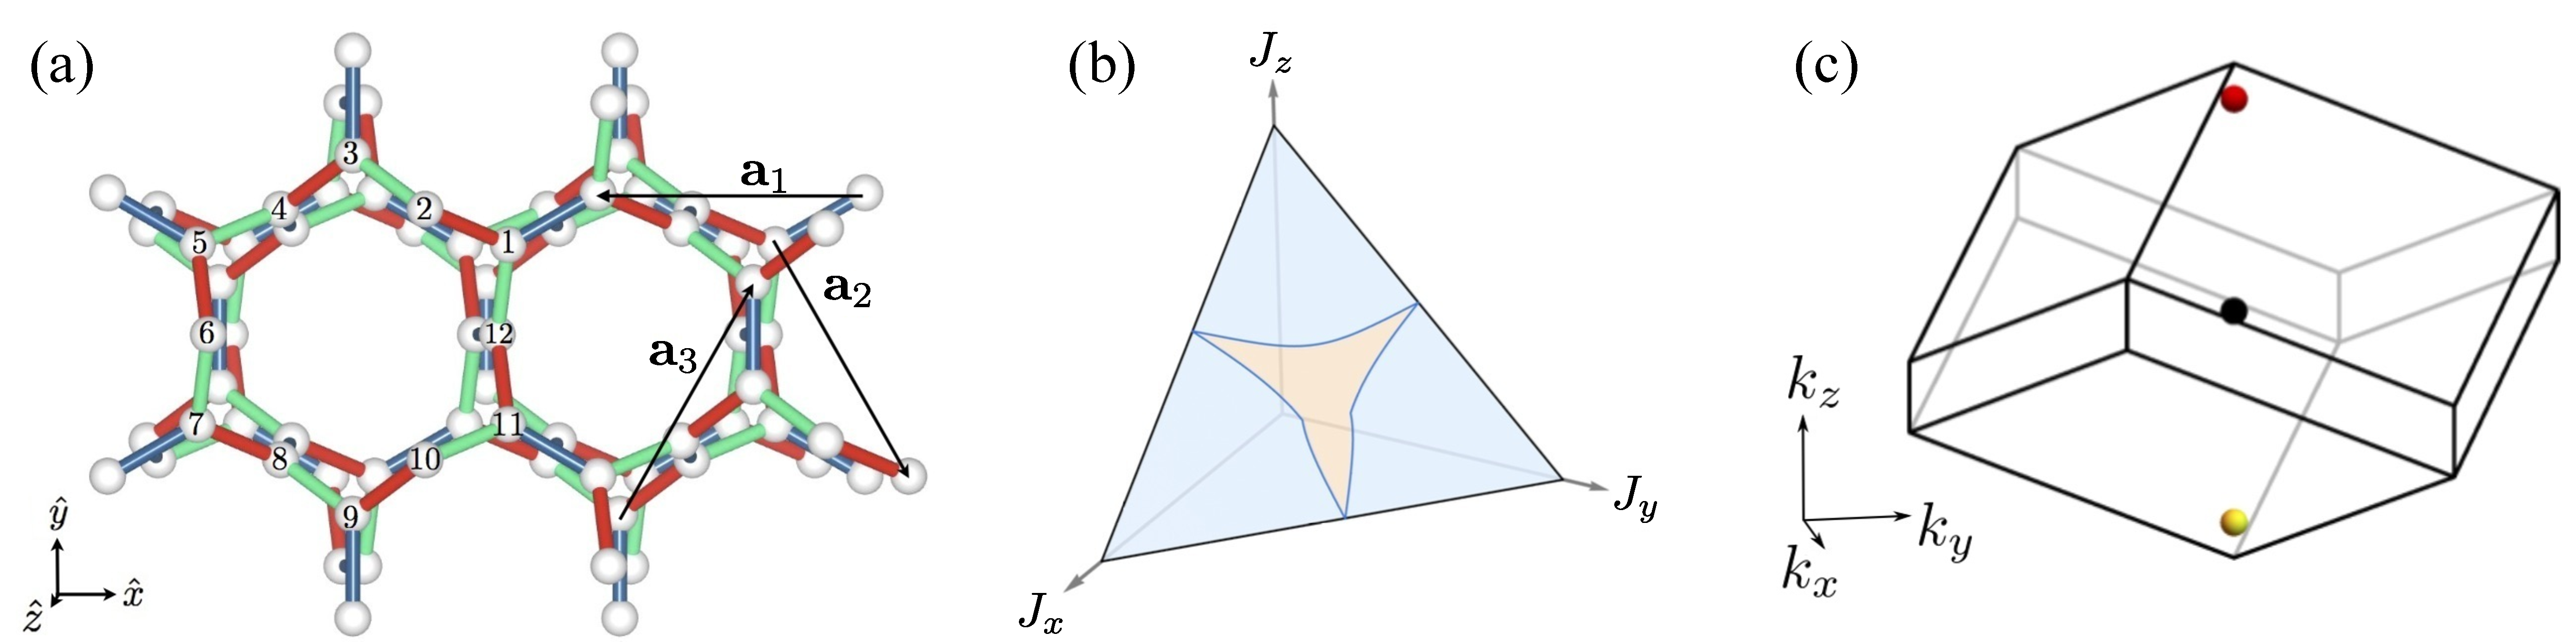
\includegraphics[width=\linewidth]{./chapter05/9_3aPanel.pdf}
	\caption{
		(a) Unit cell and translation vectors for the Kitaev model on lattice (9,3)a.
		(b) Phase diagram for lattice (9,3)a.
		The orange shaded region correspond to a gapless Weyl spin liquid phase.
		The blue shaded regions are gapped.
		(c) Brillouin zone with positions of the Weyl nodes for isotropic exchange couplings.
		Positive and negative Weyl nodes are colored red and yellow, respectively.
		A neutral combination of several Weyl nodes is denoted in black at the $\Gamma$-point.
	}
	\label{fig:chapter05_9_3aPanel}
\end{figure}
%


%
%
\subsubsection{Gauge structure}
%
%
Recalling the definition of the loop operators
%
\begin{equation}
\op{W}_p = -\prod_{\avg{j,k} \in p} (-i \sigma^{\gamma}_j \sigma^{\gamma}_k),
\end{equation}
%
one notes that for loops $p$ of odd length (as found in any \textit{non}-bipartite lattice), the corresponding loop operator is odd under time-reversal.
As a result, any eigenstate of the Kitaev Hamiltonian in a fixed flux sector breaks time-reversal symmetry spontaneously.
All eigenstates, therefore, come in degenerate time-reversal pairs with opposite $\pm \pi/2$-flux threaded through the odd-length loops.
A very similar scenario was explored in Reference~\cite{YaoPRL2007} in the discussion of a chiral spin liquid ground state emerging for a two-dimensional Kitaev model on the 3-12-12 lattice.

Lattice (9,3)a has eight loops of length 9 and one loop of length 12 per unit cell.
These nine loop operators may be combined to form two closed volumes, each of which shares a loop of length 12, leading to only \textit{six} independent loop operators of length 9 per unit cell (see Figure~\ref{fig:chapter05_9_3aPanel2} and Appendix~\ref{appendix:ThreeDimensionalKitaevModels_9_3a} for details).
In order to meaningfully discuss the \ZZ-flux of odd-length loops, one must define an orientation for the loop.
The convention used here will be to consider the loop as the boundary of an oriented surface whose normal points out of the closed volume of which it is a part.

There are only two flux configurations (not including their respective time-reversal partners) which respect the $C_3$, inversion and translations symmetries of the lattice.
These two configurations differ in that one configuration assigns $0$-flux to the loop of length 12 whereas the other assigns $\pi$-flux to the loop (see Figure~\ref{fig:chapter05_9_3aPanel2}~(b) and (c) for a visualization).
It turns out that the $0$-flux configuration has the lower energy of the two and is the flux sector which is studied in this section.
However, this $0$-flux configuration was always known \textit{not} to be the ground state flux configuration.
Unfortunately, in order to accommodate these symmetric flux sectors, the gauge field requires an enlargement of the unit cell to 96 sites, which, at the time of the publication of Reference~\cite{OBrienPRB2016} which this chapter is based off of, posed a challenge to performing a proper finite size analysis.

Subsequently, a quantum Monte Carlo study~\cite{MischenkoPRB2019} was performed to determine the ground state phase diagram for lattice (9,3)a.
It turns out that the ground state flux configuration depends greatly on the relative strengths of the exchange couplings.
The results of this study are the subject of Chapter~\ref{chapter:HypernonagonLattice}.
The vison gap for lattice (9,3)a is not reported here as calculations were not done in the ground state sector, however, it is worth noting that an elementary vison excitation results in the excitation of four loop operators (further details are given in Appendix~\ref{appendix:ThreeDimensionalKitaevModels_9_3a}).
%
\begin{figure}[tb]
	\centering
	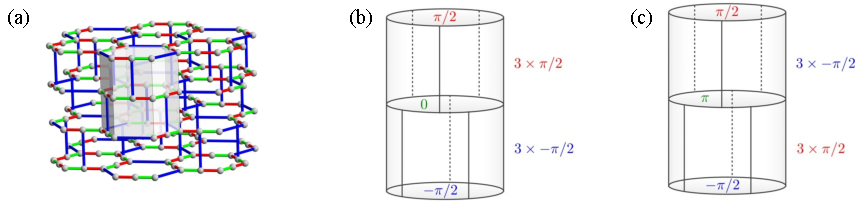
\includegraphics[width=\linewidth]{./chapter05/9_3aPanel2.pdf}
	\caption{
		(a) A deformed version of lattice (9,3)a can be obtained by coupling honeycomb layers via mid-bond sites.
		The eight elementary plaquettes of length nine per unit cell are marked by the gray transparent polygons.
		(b) $0$-flux assignment.
		(c) $\pi$-flux assignment.
	}
	\label{fig:chapter05_9_3aPanel2}
\end{figure}
%


%
%
\subsubsection{Projective symmetries}
%
%
Lattice (9,3)a is the only non-bipartite lattice considered in this project.
As such, there is no projective-representation of the time-reversal operator as time-reversal symmetry is broken on the level of the physical flux sector.
The lattice is inversion symmetric with projective representation
%
\begin{equation}
	H(\bk) = G\dag_{\mathcal{P}}~U_{\mathcal{P}}~H(-\bk)~U\dag_{\mathcal{P}}~G_{\mathcal{P}},
\end{equation}
%
where $U_{\mathcal{P}}$ is the matrix representation of the inversion operator acting on the unit cell and $G_\mathcal{P}$ is the associated gauge transformation.
The resulting energy relations are given by
%
\begin{equation}
	E_{\alpha}(\bk) = -E_{\beta}(-\bk) \qquad {\rm and } \qquad E_{\alpha}(\bk) = E_{\gamma}(-\bk),
\end{equation}
%
due to particle-hole and inversion symmetry, respectively.
Due to the lack of a projective time-reversal operator, the momentum space Hamiltonian matrix has the general form
%
\begin{equation}
	H(\bk) =
		\begin{pmatrix}
			0			&	&	A(\bk) \\
						& \ddots & \\
			A\dag(\bk)	&		 & 0
		\end{pmatrix},
\end{equation}
%
\ie, it is an inversion symmetric band Hamiltonian.


%
%
\subsubsection{Majorana band structure}
%
%
For a fixed momentum $\bk$, the general form of the Hamiltonian $H(\bk)$ for lattice (9,3)a is identical to that of lattice (8,3)b, \ie, a generic, inversion symmetric band Hamiltonian.
Just like in lattice (8,3)b, this prohibits the formation of stable Fermi surfaces, but allows for Weyl nodes pinned to zero energy.
Unlike in lattice (8,3)b, however, the Weyl nodes are not related by time-reversal symmetry.

Indeed, diagonalizing the concrete Hamiltonian for lattice (9,3)a reveals an extended gapless Weyl spin liquid phase around the point of isotropic couplings (see phase diagram in Figure~\ref{fig:chapter05_9_3aPanel}~(b)).
At the isotropic point, there are double Weyl nodes located at the positions $\pm(\bq_1 + \bq_2 + \bq_3)/3$ with charge $\mp 2$ as shown in Figure~\ref{fig:chapter05_9_3aPanel}~(c).
The fourfold degeneracy of these points is protected by the combination of particle-hole and inversion symmetries and, thus, is not affected by the addition of an external magnetic field.
Additionally, there is an eightfold degeneracy at the $\Gamma$-point consisting of a charge-neutral combination of several Weyl nodes.


%
%
% LATTICE (10,3)A %%%%%%%%%%%%%%%%%%%%%%%%%%%%%%%%%%%%%%%%%%%%%%%%%%%%%%%%%%%%%%%%%%%%%%
\subsection{Lattice (10,3)a}
\label{section:chapter05_10_3a}
%%%%%%%%%%%%%%%%%%%%%%%%%%%%%%%%%%%%%%%%%%%%%%%%%%%%%%%%%%%%%%%%%%%%%%%%%%%%%%%%%%%%%%%%
%
%
\subsubsection{Lattice information}
%
%
Lattice (10,3)a (also known in the literature as the Laves graph~\cite{HeeschZFK1933}, $K_4$ crystal~\cite{SunadaAMS2008} or hyperoctagon lattice~\cite{HermannsPRB2014}) has been previously discussed in the context of Kitaev spin liquids in Reference~\cite{HermannsPRB2014} and will be reviewed in this section.
This lattice may be viewed as another three-dimensional variant of the square-octagon lattice, wherein squares and octagons form counter-rotating spirals to form a three-dimensional lattice.
More formally, lattice (10,3)a is specified by the cubic space group $I4_{1}32$ (No. 214) and Wyckoff positions for the unit cell are $8(a)$.
The concrete choice of four site unit cell used in this work is given by the site positions
%
\begin{equation}
	\begin{matrix*}[l]
		\br_1 = \left(\frac{1}{8}, \frac{1}{8}, \frac{1}{8}\right) &
		\br_2 = \left(\frac{5}{8}, \frac{3}{8}, -\frac{1}{8}\right) \\
		&\\
		\br_3 = \left(\frac{3}{8}, \frac{1}{8}, -\frac{1}{8}\right) &
		\br_4 = \left(\frac{7}{8}, \frac{3}{8}, \frac{1}{8}\right).
	\end{matrix*}
\end{equation}
%
The lattice vectors are chosen to be
%
\begin{equation}
	\begin{matrix*}[l]
		\ba_1 = \left(1, 0, 0\right) \qquad
		\ba_2 = \left(\frac{1}{2}, \frac{1}{2}, -\frac{1}{2}\right) \qquad
		\ba_3 = \left(\frac{1}{2}, \frac{1}{2}, \frac{1}{2}\right)
	\end{matrix*}
\end{equation}
%
with the corresponding reciprocal lattice vectors
%
\begin{equation}
	\begin{matrix*}[l]
		\bq_1 = \left(2\pi, -2\pi, 0\right) \qquad
		\bq_2 = \left(0, 2\pi, -2\pi\right) \qquad
		\bq_3 = \left(0, 2\pi, 2\pi\right).
	\end{matrix*}
\end{equation}
%

The unit cell and translation vectors are illustrated in Figure~\ref{fig:chapter05_10_3aPanel}~(a).
The bonds are colored red, green and blue to indicate the assignment of $x$-, $y$- and $z$-type bonds, respectively.
This assignment of bonds is chosen to respect as many lattice symmetries as possible.
All $x$-, $y$- and $z$-bonds are related by a combination of $C_3$ and a fourfold screw symmetry.
The symmetry between $x$-, $y$- and $z$-bonds is reflected in the ground state phase diagram shown in Figure~\ref{fig:chapter05_10_3aPanel}~(b).
%
\begin{figure}[tb]
	\centering
	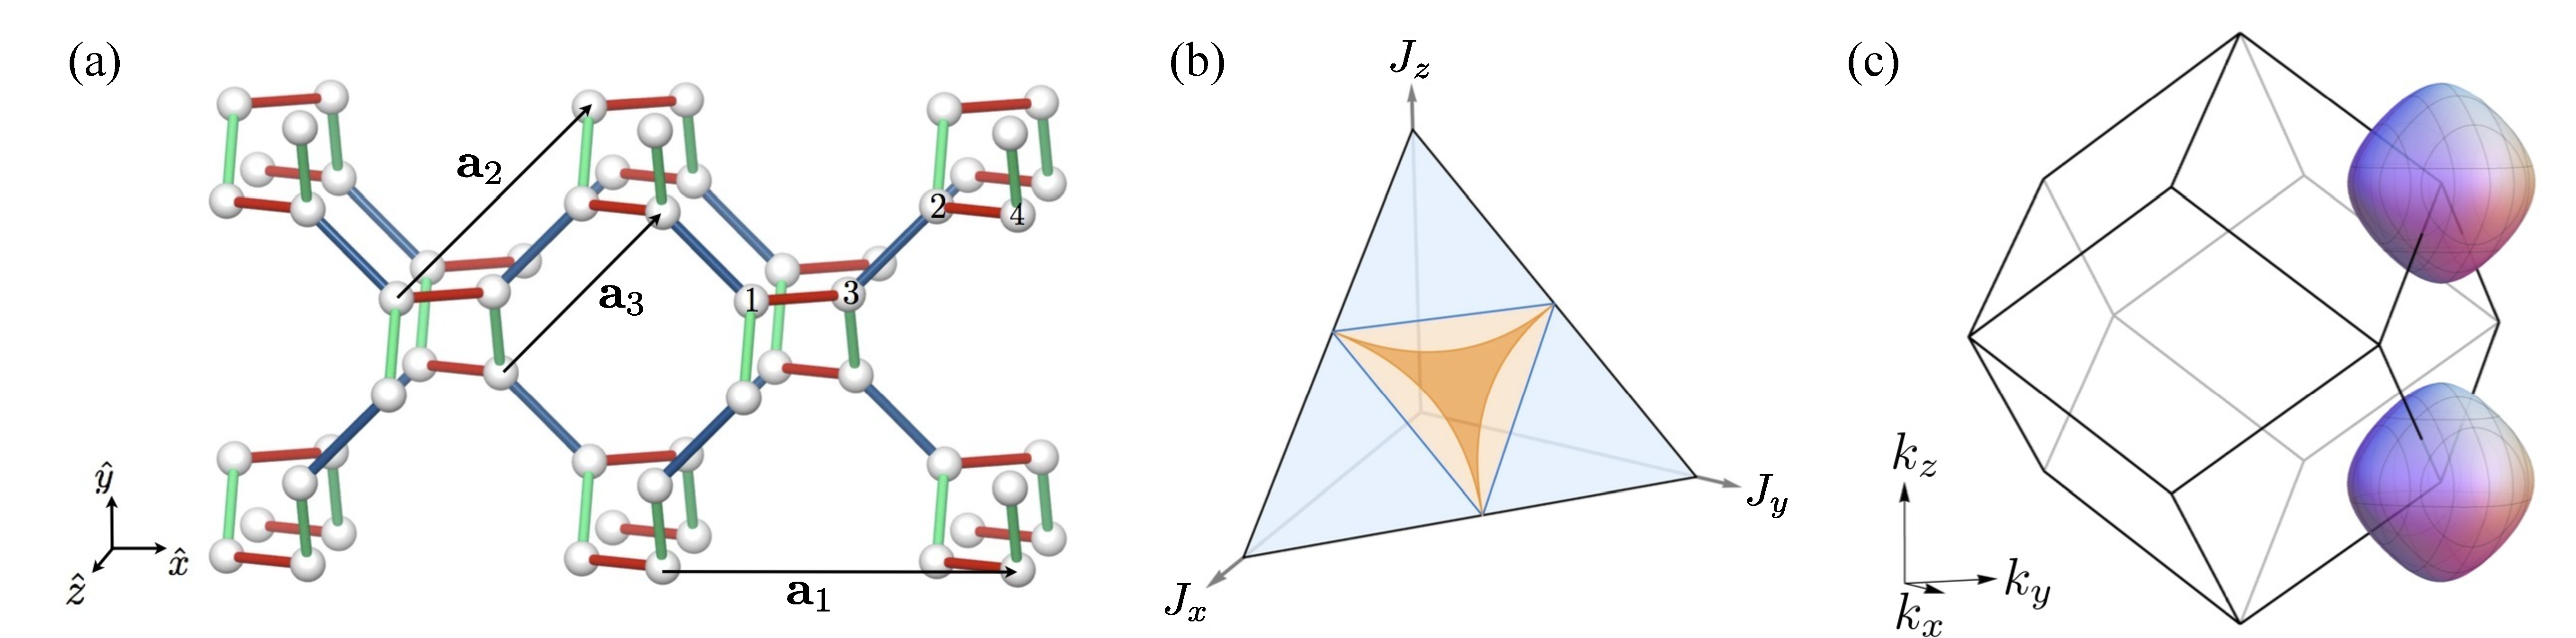
\includegraphics[width=\linewidth]{./chapter05/10_3aPanel.pdf}
	\caption{
		(a) Unit cell and translation vectors for the Kitaev model on lattice (10,3)a.
		(b) Ground state phase diagram for lattice (10,3)a.
		The region shaded darker orange has topological Fermi surfaces while the lighter orange regions have topologically-trivial Fermi surfaces.
		The blue shaded regions are gapped.
		(c) Visualization of the Majorana Fermi surfaces for isotropic exchange couplings.
	}
	\label{fig:chapter05_10_3aPanel}
\end{figure}
%


%
%
\subsubsection{Gauge structure}
%
%
Lattice (10,3)a possesses six loop operators of length 10 per unit cell.
These six loop operators may be combined to form four closed volumes leading to only \textit{two} independent loop operators per unit cell (see Appendix~\ref{appendix:ThreeDimensionalKitaevModels_10_3a} for details).
The canonical flux sector for lattice (10,3)a corresponds to $0$-flux through all elementary loops.
This results in all loop operators $\op{W}_p$ having eigenvalues $+1$.
Additionally, it has been checked numerically that the canonical flux sector is, indeed, the ground state flux sector.
The vison gap for lattice (10,3)a shown in Figure~\ref{fig:chapter05_VisonGaps}~and Table~\ref{table:chapter05_VisonGaps}~has been computed by flipping the value of $u_{jk}$ for a single $z$-bond, resulting in the excitation of ten loop operators (further details are given in Appendix~\ref{appendix:ThreeDimensionalKitaevModels_10_3a}).


%
%
\subsubsection{Projective symmetries}
%
%
Lattice (10,3)a is bipartite with different sublattices connected by the vectors $\br_0 = \ba_2$ and $\br'_0 = \ba_3$.
As a result, the projective representation of time-reversal is given by
%
\begin{equation}
	H(\bk) = G\dag_{\mathcal{T}}~H(-\bk + \bk_0)~G_{\mathcal{T}},
\end{equation}
%
where $\bk_0 = (\bq_2 + \bq_3)/2$ and the associated gauge transformation matrix is given by
%
\begin{equation}
	G_{\mathcal{T}} =
	\begin{pmatrix}
		\id	& 0    \\
		0	& -\id
	\end{pmatrix}.
\end{equation}
%
As lattice (10,3)a is chiral, the only other restriction to consider is that of particle-hole symmetry.
The resulting energy relations are given by
%
\begin{equation}
	E_{\alpha}(\bk) = -E_{\beta}(-\bk) \qquad {\rm and } \qquad E_{\alpha}(\bk) = E_{\gamma}(-\bk + \bk_0),
\end{equation}
%
due to particle-hole and time-reversal symmetry, respectively.
Due to the fact that the gauge transformation $\op{G}_{\mathcal{T}}$ relates states at momentum $\bk$ to states at momentum $\bk - \bk_0$, the momentum space Hamiltonian matrix has the form of a generic band Hamiltonian,
%
\begin{equation}
	H(\bk) =
		\begin{pmatrix}
			0			&		 & A(\bk) \\
						& \ddots &		  \\
			A\dag(\bk)	&		 & 0
		\end{pmatrix}.
\end{equation}
%


%
%
\subsubsection{Majorana band structure}
%
%
As discussed in the context of lattice (8,3)a, due to the non-trivial projective representation of time-reversal symmetry, \ie, with $\bk \neq \bm{0}$, along with the absence of inversion symmetry, lattice (10,3)a may host topological Fermi surfaces protected by Weyl-type degeneracies at finite energy.
Indeed, diagonalizing the concrete Kitaev Hamiltonian for lattice (10,3)a reveals an extended gapless phase around the point of isotropic couplings.
In the phase diagram of Figure~\ref{fig:chapter05_10_3aPanel}~(b), the darker shaded orange region corresponds to the presence of such topologically protected Fermi surfaces, whereas the lighter shaded orange regions correspond to topologically trivial Fermi surfaces.
%
\begin{figure}[tb]
	\centering
	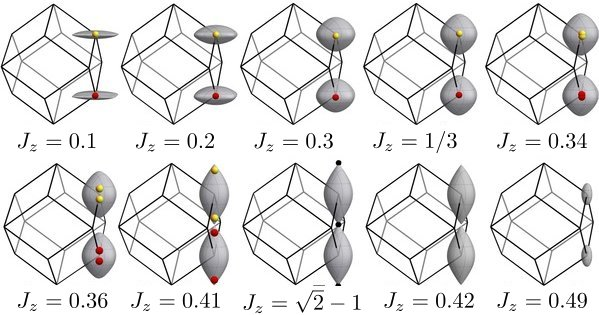
\includegraphics[width=0.55\linewidth]{./chapter05/10_3aFermiSurface.png}
	\caption{
		Evolution of the Majorana Fermi surfaces of lattice (10,3)a for varying exchange couplings $0.1 \leq J_z \leq 0.49$ and $J_x = J_y = (1 - Jz)/2$.
	}
	\label{fig:chapter05_10_3aFermiSurfaces}
\end{figure}
%

The topological Fermi surfaces are protected by Weyl-like degeneracies at finite energy.
There are a total of four such Weyl points, two of which are positively charged and two of which are negatively charged.
The four Weyl points are formed by only three bands and each Fermi surface contains two Weyl points of the same chirality.
At the isotropic point, where the Hamiltonian is highly-symmetric, pairs of Weyl points of the same chirality sit at the same momentum resulting in a threefold degeneracy which has been seen to correspond to a so-called spin-1 Weyl point~\cite{WawrzikPRB2018}.
As the couplings are tuned away from the isotropic point, however, the Weyl points are free to move through the Brillouin zone, deforming the Fermi surfaces as they do so.
Eventually, Weyl points of opposite chirality meet at high-symmetry points and mutually annihilate as the Fermi surfaces touch, thus, removing the topological protection of the Fermi surfaces.
Tuning the couplings further ultimately shrinks the Fermi surfaces to a point before gapping them out entirely (refer to Figure~\ref{fig:chapter05_10_3aFermiSurfaces} for a visualization).

The two Majorana Fermi surfaces can be mapped onto each other by the perfect nesting vector $\bk_0$ as can be seen from Figure~\ref{fig:chapter05_10_3aPanel}~(c).
As a result, the system is susceptible to a BCS-type spin-Peierls instability~\cite{HermannsPRL2015b} driven by interactions between the Majorana fermions, which can be induced by additional spin exchange such as a Heisenberg term.
A short discussion of the spin-Peierls instability occurs in Section~\ref{section:chapter05_SpinPeierls}.

Breaking time-reversal symmetry by applying an external magnetic field does not qualitatively change the nature of the nodal manifold, \ie, they remain Fermi surfaces.
However, they do deform in a non-trivial way as magnetic field strength is varied, destroying the perfect nesting condition (see Figure~\ref{fig:chapter05_10_3aPanel2}).
%
\begin{figure}[tb]
	\centering
	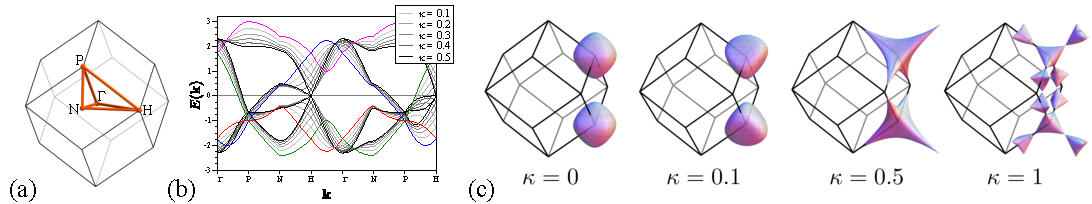
\includegraphics[width=\linewidth]{./chapter05/10_3aPanel2.pdf}
	\caption{
		(a) Brillouin zone of lattice (10,3)a with high-symmetry points.
		(b) Majorana dispersion plotted along the high-symmetry paths for varying $\kappa$.
		(c) Deformation of the Fermi surfaces in the presence of a magnetic field of varying strength $0 \leq \kappa \leq 1$.
	}
	\label{fig:chapter05_10_3aPanel2}
\end{figure}
%


%
%
% LATTICE (10,3)B %%%%%%%%%%%%%%%%%%%%%%%%%%%%%%%%%%%%%%%%%%%%%%%%%%%%%%%%%%%%%%%%%%%%%%
\subsection{Lattice (10,3)b}
\label{section:chapter05_10_3b}
%%%%%%%%%%%%%%%%%%%%%%%%%%%%%%%%%%%%%%%%%%%%%%%%%%%%%%%%%%%%%%%%%%%%%%%%%%%%%%%%%%%%%%%%
%
%
\subsubsection{Lattice information}
%
%
Lattice (10,3)b is probably the best known three-dimensional tricoordinated lattice and is typically referred to in the literature as the hyperhoneycomb lattice~\cite{TakayamaPRL2015}.
The Kitaev model for this lattice has been discussed extensively~\cite{MandalPRB2009,HermannsPRB2014,LeePRB2014,KimchiPRB2014,NasuPRB2014} in the context of the iridate material \betaLithiumIridate~\cite{TakayamaPRL2015}.

The most symmetric form of lattice (10,3)b can best be visualized as parallel $xy$-zigzag chains along two distinct direction which are coupled by $z$-type bonds
It may be viewed as a close relative of lattice (10,3)c which is made up of three parallel $xy$-zigzag chains which are coupled by $z$-type bonds (see Figure~\ref{fig:chapter05_10_3bcComparison} for a comparison).
Formally, lattice (10,3)b is specified by the tetragonal space group $I4_{1}/ambd$ (No. 141) with $c/a = 2\sqrt{3}$ and Wyckoff positions for the unit cell are $8(e)$ with $z = 1/12$.
The concrete choice of four site unit cell used in this work is given by the site positions
%
\begin{equation}
	\begin{matrix*}[l]
		\br_1 = \left(0, 0, 0\right) &
		\br_2 = \left(1, 2, 1\right) \\
		&\\
		\br_3 = \left(1, 1, 0\right) &
		\br_4 = \left(2, 3, 1\right).
	\end{matrix*}
\end{equation}
%
The lattice vectors are chosen to be
%
\begin{equation}
	\begin{matrix*}[l]
		\ba_1 = \left(-1, 1, -2\right) \qquad
		\ba_2 = \left(-1, 1, 2\right) \qquad
		\ba_3 = \left(2, 4, 0\right)
	\end{matrix*}
\end{equation}
%
with the corresponding reciprocal lattice vectors
%
\begin{equation}
	\begin{matrix*}[l]
		\bq_1 = \left(-\frac{2\pi}{3}, \frac{\pi}{3}, -\frac{\pi}{2}\right) \qquad
		\bq_2 = \left(-\frac{2\pi}{3}, \frac{\pi}{3}, \frac{\pi}{2}\right) \qquad
		\bq_3 = \left(\frac{\pi}{3}, \frac{\pi}{3}, 0\right).
	\end{matrix*}
\end{equation}
%

The unit cell and translation vectors are illustrated in Figure~\ref{fig:chapter05_10_3bPanel}~(a).
The bonds in the figure are colored red, green and blue to indicate the assignment of $x$-, $y$- and $z$-type bonds, respectively.
This assignment of bonds is chosen to respect as many of the lattice symmetries as possible.
All $x$- and $y$-bonds are related by a combination of $C_2$ and a two-fold screw symmetry.
All $z$-bonds are related to each other by inversion symmetry, but are not related to any other bond type by lattice symmetries.
The symmetry between $x$- and $y$-bonds is reflected in the ground state phase diagram shown in Figure~\ref{fig:chapter05_10_3bPanel}~(b).
%
\begin{figure}[tb]
	\centering
	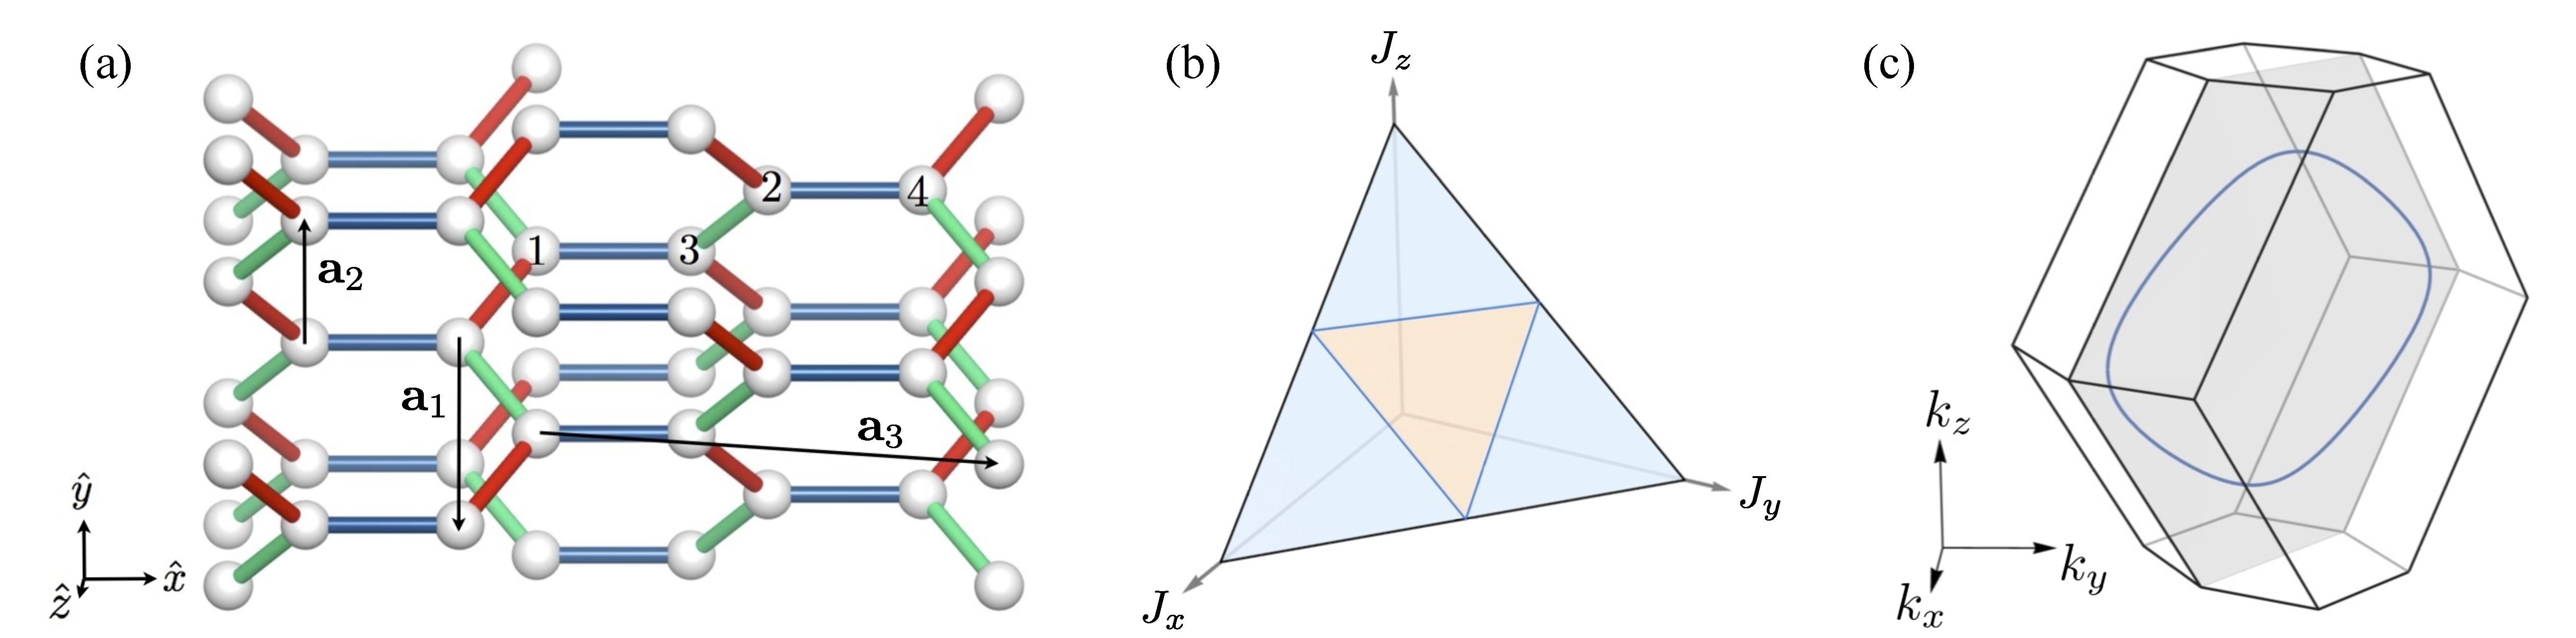
\includegraphics[width=\linewidth]{./chapter05/10_3bPanel.pdf}
	\caption{
		(a) Unit cell and translation vectors for the Kitaev model on lattice (10,3)b.
		(b) Ground state phase diagram for lattice (10,3)b.
		The region shaded orange corresponds to a gapless phase with a nodal line.
		The blue shaded regions are gapped.
		(c) At the isotropic point, the nodal line (marked in blue) is located in the $k_x + k_y = 0$ plane (indicated in gray).
	}
	\label{fig:chapter05_10_3bPanel}
\end{figure}
%


%
%
\subsubsection{Gauge structure}
%
%
Lattice (10,3)b possesses four loop operators of length 10 per unit cell.
These four loop operators can be combined to form two closed volumes, leading to only \textit{two} independent loop operators per unit cell (see Appendix~\ref{appendix:ThreeDimensionalKitaevModels_10_3b} for details).
The canonical flux sector for lattice (10,3)b corresponds to $0$-flux through all elementary loops.
This results in all loop operators $\op{W}_p$ having eigenvalues $+1$.
Additionally, it has been checked numerically that the canonical flux sector is, indeed, the ground state flux sector.
The vison gap for lattice (10,3)b shown in Figure~\ref{fig:chapter05_VisonGaps}~and Table~\ref{table:chapter05_VisonGaps}~has been computed by flipping the value of $u_{jk}$ for a single $z$-bond, resulting in the excitation of six loop operators (further details are given in Appendix~\ref{appendix:ThreeDimensionalKitaevModels_10_3b}).


%
%
\subsubsection{Projective symmetries}
%
%
%
\begin{figure}[tb]
	\centering
	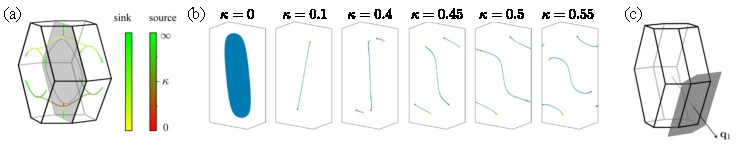
\includegraphics[width=\linewidth]{./chapter05/10_3bPanel2.pdf}
	\caption{
		(a) Evolution of Weyl nodes of lattice (10,3)b in the presence of a magnetic field of varied strength $0 \leq \kappa < \infty$.
		(b) Corresponding Fermi arc evolution.
		(c) Visualization of the surface Brillouin zone for the 100-surface.
	}
	\label{fig:chapter05_10_3bPanel2}
\end{figure}
%
Lattice (10,3)b is bipartite with sublattices having the same translation symmetry as the elementary unit cell.
The resulting projective representation of time-reversal is given by
%
\begin{equation}
	H(\bk) = G\dag_{\mathcal{T}}~H(-\bk)~G_{\mathcal{T}},
\end{equation}
%
where the associated gauge transformation matrix is given by
%
\begin{equation}
	G_{\mathcal{T}} =
		\begin{pmatrix}
			\id & 0 \\
			0	& -\id
		\end{pmatrix}.
\end{equation}
%
Furthermore, the lattice is inversion symmetric with projective representation
%
\begin{equation}
	H(\bk) = G\dag_{\mathcal{P}}~U_{\mathcal{P}}~H(-\bk)~U\dag_{\mathcal{P}}~G_{\mathcal{P}},
\end{equation}
%
where $U_{\mathcal{P}}$ is the matrix representation of the inversion operator acting on the unit cell, and the associated gauge transformation matrix $G_{\mathcal{P}}$ is identical to $G_{\mathcal{T}}$ for the gauge \textit{Ansatz} used here.
The resulting energy relations are given by
%
\begin{equation}
	E_{\alpha}(\bk) = -E_{\beta}(-\bk) \qquad {\rm and } \qquad E_{\alpha}(\bk) = E_{\gamma}(-\bk),
\end{equation}
%
where the first relation is due to particle-hole symmetry and the second is enforced individually by both time-reversal and inversion symmetry.
Due to the fact that the gauge transformation $\op{G}_{\mathcal{T}}$ is constant as a function of unit cell position, the momentum space Hamiltonian matrix has the block off-diagonal form
%
\begin{equation}
	H(\bk) =
		\begin{pmatrix}
			0			& A(\bk) \\
			A\dag(\bk)	& 0
		\end{pmatrix}.
\end{equation}
%
\newpage


%
%
\subsubsection{Majorana band structure}
%
%
As was the case for lattice (8,3)c, a trivially implemented projective time-reversal symmetry leads to nodal lines being the only stable zero energy manifolds for lattice (10,3)b.
These nodal lines are characterized by an integer invariant and are protected by the presence of time-reversal symmetry.

Diagonalizing the concrete Kitaev Hamiltonian for lattice (10,3)b, indeed, reveals an extended gapless phase around the point of isotropic couplings (see Figure~\ref{fig:chapter05_10_3bPanel}~(b)), where the zero modes correspond to a contractible loop in the Brillouin zone.
At the isotropic point, this line lies in the plane defined by $k_x + k_y = 0$.

Breaking time-reversal explicitly by introducing an external magnetic field removes the symmetry protection of the nodal line, gapping it to a pair of Weyl nodes due to the presence of a trivially implemented projective inversion symmetry~\cite{HermannsPRL2015}.
This is precisely the scenario which was seen to occur for lattice (8,3)c, above.
For small values of $\kappa$, the Weyl nodes move along the $z$-axis.
At $\kappa = \frac{1}{2} \sqrt{\frac{3}{5}}$, four more Weyl nodes appear.
The full evolution of the Weyl nodes for $0 \leq \kappa < \infty$ along with the corresponding Fermi arc surfaces states are pictured in Figure~\ref{fig:chapter05_10_3bPanel2}~(a) and (b).
The trajectory of negatively charged Weyl nodes changes colors from yellow to green as $\kappa$ is increased, whereas the trajectory of positively charged Weyl nodes changes from red to green.
While the Weyl nodes which move along the $z$-axis recombine at $\kappa \rightarrow \infty$, the ones on the front/back faces of the Brillouin zone do not.
Instead, the velocity vectors of the isolated Weyl nodes vanish, collapsing the bulk gap to a nodal line.
Additionally, one notes that for the pure Kitaev model, \ie, with $\kappa = 0$, there is an entire puddle of zero modes which appear in the surface Brillouin zone.
These zero modes appear within the area bounded by the projection of the bulk nodal line to the surface Brillouin zone and are associated to the non-vanishing integer invariant due to the presence of time-reversal symmetry.


%
%
% LATTICE (10,3)C %%%%%%%%%%%%%%%%%%%%%%%%%%%%%%%%%%%%%%%%%%%%%%%%%%%%%%%%%%%%%%%%%%%%%%
\subsection{Lattice (10,3)c}
\label{section:chapter05_10_3c}
%%%%%%%%%%%%%%%%%%%%%%%%%%%%%%%%%%%%%%%%%%%%%%%%%%%%%%%%%%%%%%%%%%%%%%%%%%%%%%%%%%%%%%%%
%
%
\subsubsection{Lattice information}
%
%
As mentioned above lattice (10,3)c is in some sense a relative of lattice (10,3)b (see discussion at the beginning of Section~\ref{section:chapter05_10_3b} and Figure~\ref{fig:chapter05_10_3bcComparison}).
One significant distinction between the two lattices is that, whereas lattice (10,3)b is inversion symmetric, lattice (10,3)c is chiral.
%
\begin{figure}[tb]
	\centering
	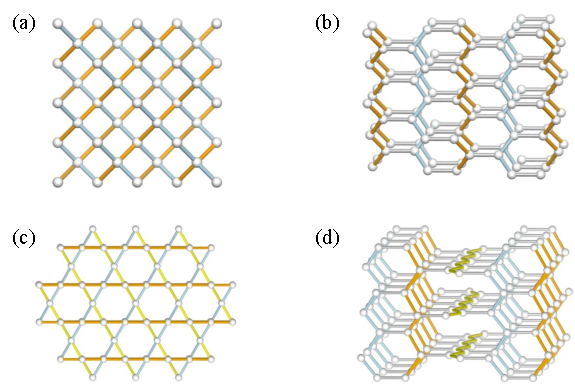
\includegraphics[width=0.6\linewidth]{./chapter05/10_3bcComparison.pdf}
	\caption{
		Comparison of lattice (10,3)b -- shown in (a) and (b) -- and lattice (10,3)c -- shown in (c) and (d).
	}
	\label{fig:chapter05_10_3bcComparison}
\end{figure}
%

More formally, lattice (10,3)c is specified by the trigonal space group $P3_{1}12$ (No. 151) with $c/a = 3\sqrt{3}/2$ and Wyckoff positions for the unit cell are $6(c)$ with $x = 1/3$, $y = 1/6$ and $z = 1/9$.
The concrete choice of unit cell specified in this work has six sites per unit cell at positions
%
\begin{equation}
	\begin{matrix*}[l]
		\br_1 = \left(\frac{1}{4}, \frac{1}{4\sqrt{3}}, \frac{1}{2\sqrt{3}}\right) &
		\br_2 = \left(\frac{3}{4}, \frac{1}{4\sqrt{3}}, \frac{2}{\sqrt{3}}\right) &
		\br_3 = \left(\frac{1}{2}, \frac{1}{\sqrt{3}}, \frac{7}{2\sqrt{3}}\right) \\
		&\\
		\br_4 = \left(\frac{3}{4}, \frac{1}{4\sqrt{3}}, \frac{1}{\sqrt{3}}\right) &
		\br_5 = \left(\frac{1}{2}, \frac{1}{\sqrt{3}}, \frac{5}{2\sqrt{3}}\right) &
		\br_6 = \left(\frac{1}{4}, \frac{1}{4\sqrt{3}}, \frac{4}{\sqrt{3}}\right).
	\end{matrix*}
\end{equation}
%
The lattice vectors are chosen to be
%
\begin{equation}
	\begin{matrix*}[l]
		\ba_1 = \left(1, 0, 0\right) \qquad
		\ba_2 = \left(-\frac{1}{2}, \frac{\sqrt{3}}{2}, 0\right) \qquad
		\ba_3 = \left(0, 0, \frac{3\sqrt{3}}{2}\right)
	\end{matrix*}
\end{equation}
%
with the corresponding reciprocal lattice vectors
%
\begin{equation}
	\begin{matrix*}[l]
		\bq_1 = \left(2\pi, \frac{2\pi}{\sqrt{3}}, 0\right) \qquad
		\bq_2 = \left(0, \frac{4\pi}{\sqrt{3}}, 0\right) \qquad
		\bq_3 = \left(0, 0, \frac{4\pi}{3\sqrt{3}}\right).
	\end{matrix*}
\end{equation}
%
As will be discussed in the following section, this unit cell must be enlarged in order to accommodate the ground state flux sector.

The unit cell and translation vectors are illustrated in Figure~\ref{fig:chapter05_10_3cPanel}~(a).
The bonds in the figure are colored red, green and blue, to indicate the assignment of $x$-, $y$- and $z$-type bonds, respectively.
This assignment of bonds is chosen to respect as many of the lattice symmetries as possible.
All $x$- and $y$-bonds are related by a threefold screw symmetry.
All $z$-bonds are related to each other by the same screw symmetry, but not to any other type of bond.
The symmetry between $x$- and $y$-bonds is reflected in the ground state phase diagram shown in Figure~\ref{fig:chapter05_10_3cPanel}~(b).


%
%
\subsubsection{Gauge structure}
%
%
Lattice (10,3)c possesses three loop operators of length 10 and three of length 12 per unit cell.
These six loop operators can be combined to form three closed volumes, leading to only \textit{three} independent loop operators per unit cell (see Appendix~\ref{appendix:ThreeDimensionalKitaevModels_10_3c} for details).
The canonical flux sector for lattice (10,3)c corresponds to $0$-flux through all loops of length 10 and $\pi$-flux through all loops of length 12.
This results in all loop operators $\op{W}_p$ having eigenvalues $+1$.
Additionally, it has been checked numerically that the canonical flux sector is, indeed, the ground state flux sector.
In order to fix a gauge \textit{Ansatz} compatible with the ground state flux sector, however, the unit cell must be doubled in the 010-direction (see Appendix~\ref{appendix:ThreeDimensionalKitaevModels_10_3c} for definition of the expanded unit cell).
The vison gap for lattice (10,3)c shown in Figure~\ref{fig:chapter05_VisonGaps}~and Table~\ref{table:chapter05_VisonGaps}~has been computed by flipping the value of $u_{jk}$ for a single $z$-bond, resulting in the excitation of fourteen loop operators (further details are given in Appendix~\ref{appendix:ThreeDimensionalKitaevModels_10_3c}).
%
\begin{figure}[tb]
	\centering
	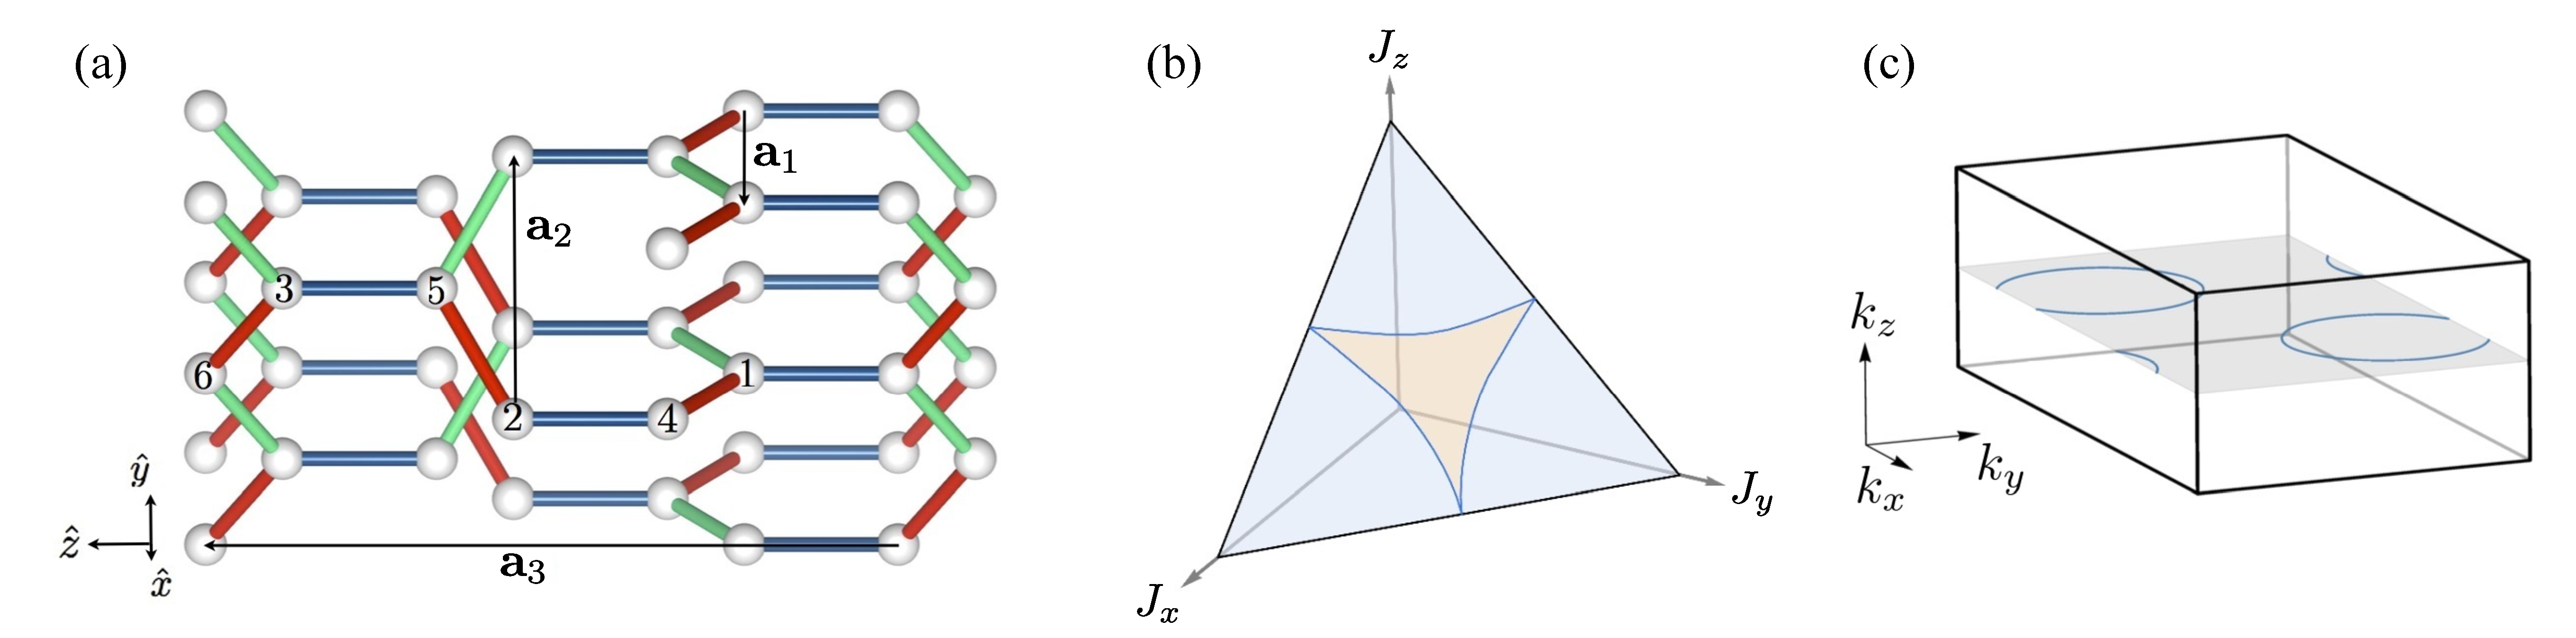
\includegraphics[width=\linewidth]{./chapter05/10_3cPanel.pdf}
	\caption{
		(a) Unit cell and translation vectors for the Kitaev model on lattice (10,3)c.
		(b) Ground state phase diagram for lattice (10,3)c.
		The region shaded orange corresponds to a gapless phase with nodal lines.
		The blue shaded regions are gapped.
		(c) At the isotropic point, the nodal lines (marked in blue) are located in the $k_z = 0$ plane (indicated in gray).
	}
	\label{fig:chapter05_10_3cPanel}
\end{figure}
%


%
%
\subsubsection{Projective symmetries}
%
%
Lattice (10,3)c is bipartite with sublattices having the same translation symmetry as the elementary unit cell.
The resulting projective representation of time-reversal is given by
%
\begin{equation}
	H(\bk) = G\dag_{\mathcal{T}}~H(-\bk)~G_{\mathcal{T}},
\end{equation}
%
where the associated gauge transformation matrix is given by
%
\begin{equation}
	G_{\mathcal{T}} =
		\begin{pmatrix}
			\id & 0 \\
			0	& -\id
		\end{pmatrix}.
\end{equation}
%
As mentioned above, the gauge \textit{Ansatz} in the canonical flux sector necessarily doubles the unit cell in the 010-direction, resulting in a gauge \textit{Ansatz} which is not \textit{invariant} under translations along $\ba_2$.
It is, however, \textit{symmetric} under translations along $\ba_2$ when the corresponding gauge transformation is accounted for.
This gauge transformation alternates in sign as a function of unit cell position $\br$ in the $\ba_1$ direction, \ie,
\begin{align}
	G_{T_2}(\br) &= -G_{T_2}(\br + \ba_1) \nonumber\\
				 &= \exp{(i \bk'_0 \cdot \br)} G_{T_2}(\br),
\end{align}
where $\bk'_0 = \bq_1 / 2$.
As lattice (10,3)c is chiral, the only other restriction to consider is that of particle-hole symmetry.
The resulting energy relations are given by
%
\begin{equation}
	E_{\alpha}(\bk) = - E_{\beta}(-\bk) \qquad E_{\alpha}(\bk) = E_{\gamma}(-\bk) \qquad E_{\alpha}(\bk) = E_{\delta}(\bk + \bk'_0),
\end{equation}
%
due to particle-hole, time-reversal and translation symmetry, respectively.
Due to the fact that the gauge transformations $\op{G}_{\mathcal{T}}$ is constant as a function of unit cell position, the momentum space Hamiltonian matrix has the block off-diagonal form
%
\begin{equation}
	H(\bk) =
		\begin{pmatrix}
			0			& A(\bk) \\
			A\dag(\bk)	& 0
		\end{pmatrix}.
\end{equation}
%


%
%
\subsubsection{Majorana band structure}
%
%
As was the case for lattices (8,3)c and (10,3)b, a trivially implemented projective time-reversal symmetry leads to nodal lines being the only stable zero energy manifolds for lattice (10,3)c.
These nodal lines are characterized by an integer invariant and are protected by the presence of time-reversal symmetry.

Diagonalizing the concrete Kitaev Hamiltonian for lattice (10,3)c, indeed, reveals an extended gapless phase around the point of isotropic couplings (see Figure~\ref{fig:chapter05_10_3cPanel}~(b)), where the zero modes correspond to two closed nodal lines.
These nodal lines are related by the nesting vector $\bk'_0 = \bq_1 / 2$ due to the projective representation of translation symmetry.
For isotropic couplings, these nodal lines lie in the plane defined by $k_z = 0$ (see Figure~\ref{fig:chapter05_10_3cPanel}~(c) -- note that the Brillouin zone is for the expanded unit cell).
Breaking time-reversal symmetry explicitly by introducing an external magnetic field removes the symmetry protection of the nodal lines, gapping each line to six Weyl nodes related by a threefold screw axis, for a total of twelve Weyl nodes.

However, in contrast to lattices (8,3)c and (10,3)b, lattice (10,3)c is chiral.
This lack of inversion symmetry allows the Weyl-degeneracies to move away from zero energy as $\kappa$ is increased, resulting in twelve Fermi surfaces.
As each Fermi surface is generated by a Weyl-like degeneracy, it inherits a topological protection.
For a visualization of the formation of the Fermi surfaces, refer to Figure~\ref{fig:chapter05_10_3cPanel2}.
Note that lattice (10,3)c represents the only example presented in this work for which the breaking of time-reversal symmetry actually \textit{increases} the density of states at zero energy.
%
\begin{figure}[tb]
	\centering
	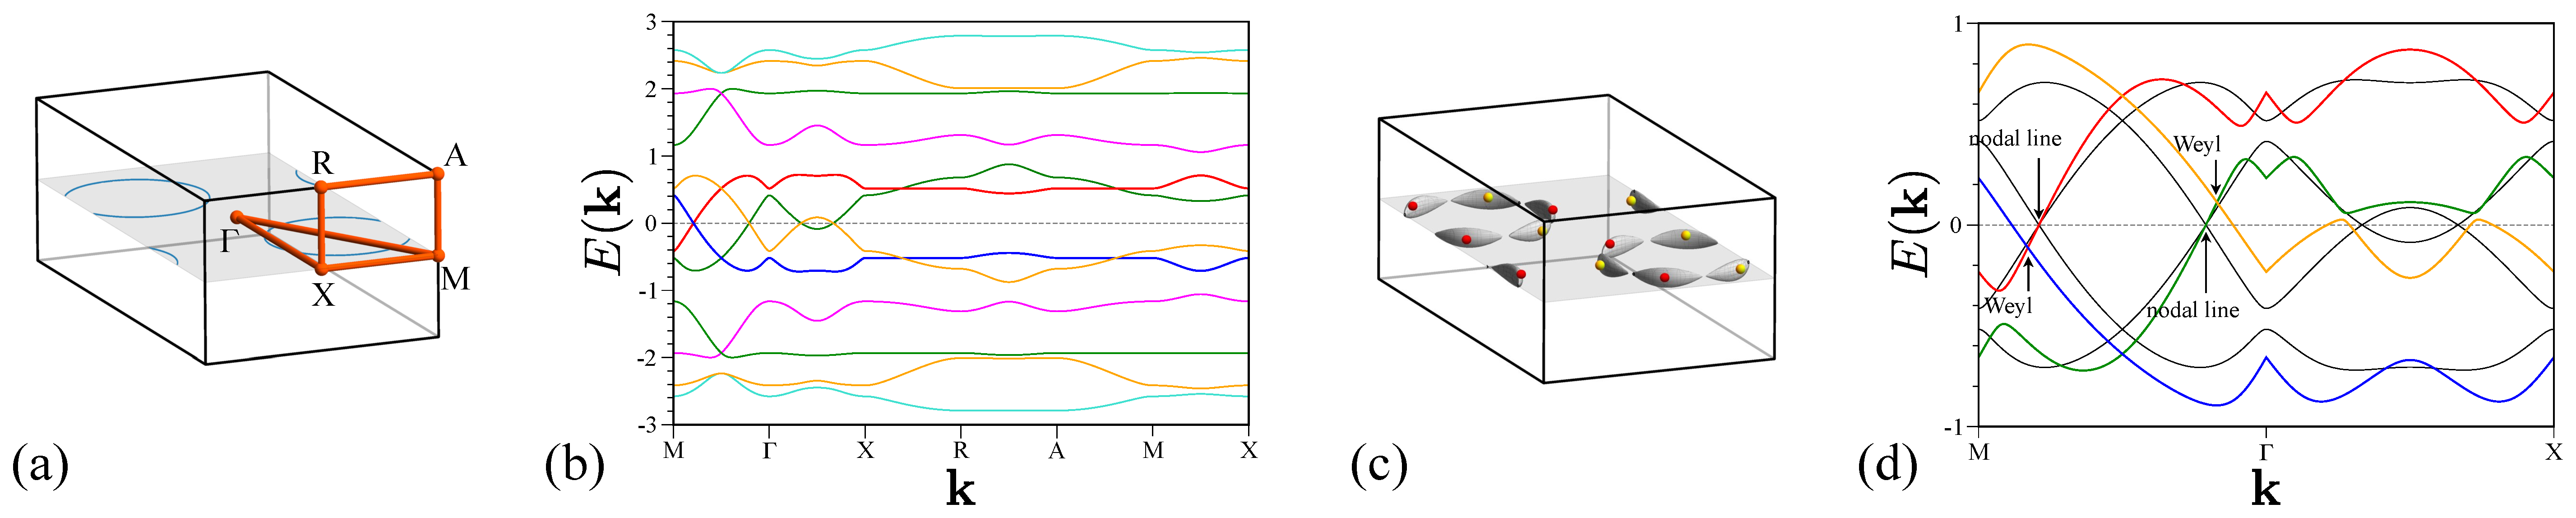
\includegraphics[width=\linewidth]{./chapter05/10_3cPanel2.pdf}
	\caption{
		(a) Brillouin zone of expanded unit cell of lattice (10,3)c with high-symmetry points.
		(b) Majorana dispersion plotted along the high-symmetry paths for $\kappa = 0$.
		(c) Majorana Fermi surfaces for $\kappa = 0.2$ enclosing finite-energy topological degeneracies denoted by red and yellow spheres.
		(d) Majorana dispersion plotted along high-symmetry path.
		The black lines indicates the nodal line dispersion for $\kappa = 0$, whereas, the colored lines indicate the Fermi surface dispersion with topological degeneracies at finite energy for $\kappa = 0.2$.
	}
	\label{fig:chapter05_10_3cPanel2}
\end{figure}
%


%
%
%%%%%%%%%%%%%%%%%%%%%%%%%%%%%%%%%%%%%%%%%%%%%%%%%%%%%%%%%%%%%%%%%%%%%%%%%%%%%%%%%%%%%%%%
\section{Spin-Peierls instabilities}
\label{section:chapter05_SpinPeierls}
%%%%%%%%%%%%%%%%%%%%%%%%%%%%%%%%%%%%%%%%%%%%%%%%%%%%%%%%%%%%%%%%%%%%%%%%%%%%%%%%%%%%%%%%
%
%
While the above discussion focuses solely on the pure Kitaev model, it is necessary to understand the effects of additional interactions, \eg, Heisenberg exchange.
Such additional spin-exchange terms have two generic consequences.
First, they do not commute with the gauge variables, making the gauge field dynamic.
Second, they induce interactions between the itinerant Majorana fermions.
For sufficiently small perturbations, one may ignore the first effect as vison excitations remain gapped.
The effect of interactions, however, depends crucially on the nature of the gapless modes.

For quantum spin liquids with a nodal line or Weyl nodes, a scaling analysis as performed in Reference~\cite{LeePRB2014} shows that the interaction terms are irrelevant in the renormalization group sense.
Thus, such spin liquids are stable against small perturbations.
For quantum spin liquids with a Majorana Fermi surface, however, such interactions are marginal.
A careful analysis~\cite{HermannsPRL2015b} for lattice (10,3)a has shown that time-reversal invariant interactions generically destabilize the Majorana Fermi surfaces even for infinitesimal interaction strength.
In this case, the Fermi surfaces are gapped out with the exception of an odd number of nodal lines.
The following shall serve as a brief review of the underlying mechanism and main features of this instability, which is referred to as a spin-Peierls BCS instability.

As was shown in Section~\ref{section:chapter05_3DKitaevModels}, stable Majorana Fermi surfaces only occur in a pure Kitaev model when the projective time-reversal symmetry is implemented non-trivially, \ie, with non-vanishing $\bk_0$.
Combined with particle-hole symmetry, the result is that the Majorana Fermi surfaces exhibit a perfect nesting, \ie, $E(\bk) = -E(\bk + \bk_0)$.
This perfect nesting is visualized for lattices (10,3)a and (8,3)a in Figure~\ref{fig:chapter05_SpinPeierls}~(a) and (b), respectively.
%
\begin{figure}[tb]
	\centering
	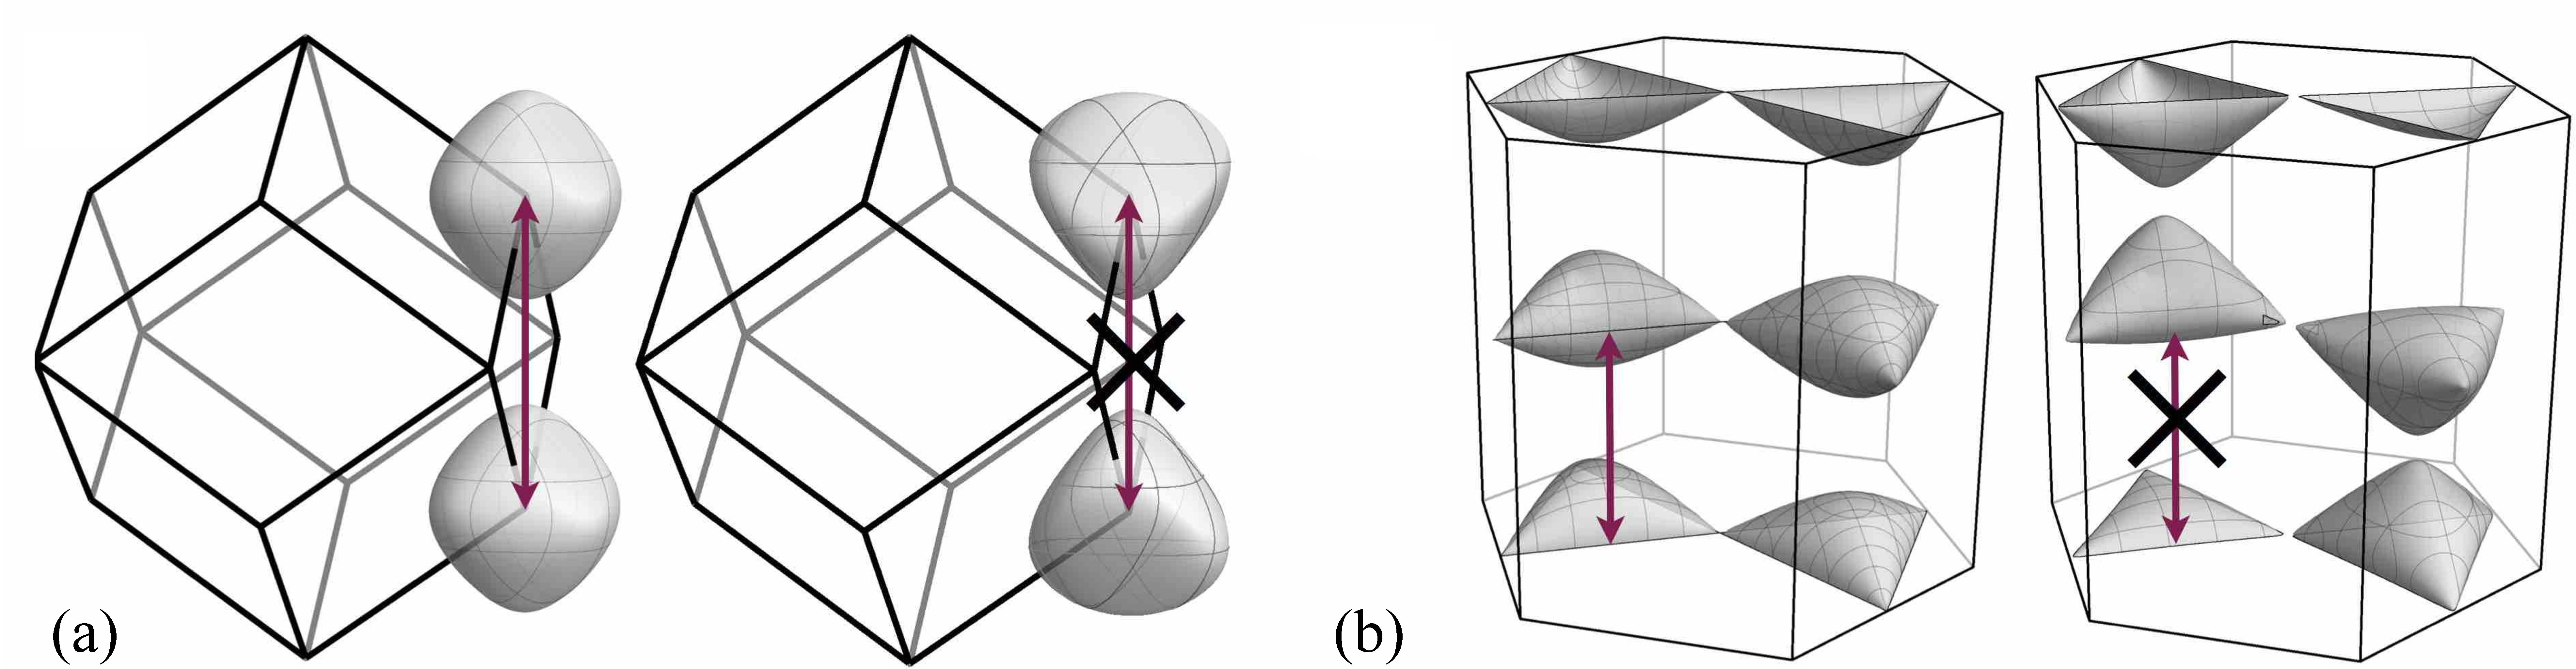
\includegraphics[width=\linewidth]{./chapter05/SpinPeierls.pdf}
	\caption{
		Effects of time-reversal symmetry breaking on (a) lattice (10,3)a and (b) lattice (8,3)a.
		Figures on the left show the time-reversal invariant system, whereas figures on the right show the system with time-reversal symmetry broken for $\kappa = 0.1$.
		Breaking time-reversal symmetry destroys the perfect nesting condition with wave vector $\bk_0$, denoted by the arrow.
	}
	\label{fig:chapter05_SpinPeierls}
\end{figure}
%

It is convenient to express the system in terms of its \textit{complex} fermionic single-particle eigenstates corresponding to the creation/annihilation operators $f_{\alpha}(\bk) = f\dag_{\beta}(-\bk)$.
The $2n$ Majorana Fermi surfaces are then combined into $n$ complex Fermi surfaces and the perfect nesting condition becomes the usual BCS pairing condition $E(\bk_0/2 + \bk) = E(\bk_0/2 - \bk)$ centered around $\bk_0/2$.
Note that there is no $U(1)$ symmetry in this system.
Instead, a non-vanishing pair correlator
%
\begin{equation}
	\avg{f\dag_{\alpha}(\bk_0/2 + \bk) f\dag_{\beta}(\bk_0/2 - \bk)}
\end{equation}
%
breaks translation symmetry spontaneously.
The resulting dimerization is reflected, \eg, in the spin-spin correlations which acquire a staggered component.
Due to the spontaneous breaking of translation symmetry, this BCS-type instability shows similar features to the usual spin-Peierls instability, except that the dimerization occurs for infinitesimal interaction strength.
As shown in Reference~\cite{HermannsPRL2015b}, any time-reversal invariant interaction will, independent of microscopic detail, result in this kind of instability.
For the Kitaev model on lattice (10,3)a, time-reversal symmetry ensures that the Fermi surfaces cannot be gapped out completely and an odd number of nodal lines always remains.
On lattice (8,3)a, however, the presence of \textit{four} rather than two Majorana Fermi surfaces allows, in principle, for interactions to gap the system out entirely.

One way to stabilize the Fermi surfaces is by breaking time-reversal symmetry.
This leads to a deformation of the Fermi surfaces, spoiling the perfect nesting condition (see Figure~\ref{fig:chapter05_SpinPeierls}), \ie, translation by $\bk_0$ in momentum space no longer maps the Fermi surfaces onto each other.
As a result, the BCS instability is cut off at sufficiently low temperatures and the Fermi surface is restored.


%
%
%%%%%%%%%%%%%%%%%%%%%%%%%%%%%%%%%%%%%%%%%%%%%%%%%%%%%%%%%%%%%%%%%%%%%%%%%%%%%%%%%%%%%%%%
\section{Summary and outlook}
\label{section:chapter05_Conclusion}
%%%%%%%%%%%%%%%%%%%%%%%%%%%%%%%%%%%%%%%%%%%%%%%%%%%%%%%%%%%%%%%%%%%%%%%%%%%%%%%%%%%%%%%%
%
%
The work reported in this chapter accomplished several tasks.
First, a number of three-dimensional tricoordinated lattices were considered for the first time in the context of frustrated magnetism.
Second, the Kitaev honeycomb model was investigated for quantum spin-1/2 moments on these lattices with a focus on the gapless spin liquid phase.
Additionally the effects of applying a weak, external magnetic field were considered.
This analysis revealed a rich and varied physics where the low-energy, fermionic quasiparticle excitations formed either full two-dimensional Fermi surfaces, one-dimensional nodal lines or topologically protected Weyl nodes, depending on the lattice under consideration.

Most importantly, this work established a systematic method for classifying and predicting the Fermi surface topology of these Kitaev spin liquids by making use of the projective symmetry group.
The physical symmetry group considered is given by
%
\begin{equation}
SG = \avg{\{ \op{T}_1, \op{T}_2, \op{T}_3, \op{\mathcal{P}}, \op{\mathcal{T}} \}}
\end{equation}
%
and those of its subgroups which include the translation symmetries.
By finding the projective representation of the physical symmetries in a fixed gauge sector, one may identify restrictions that a given projective representation places on the low-energy physics of the model.

The ideas behind this classification, which are scattered throughout the chapter, are now recapitulated below.
With the exception of lattice (10,3)c, the gauge \textit{Ans\"atze} used are all translationally invariant, allowing for the block diagonalization of the Hamiltonian into momentum sectors $H(\bk)$.
Note that such a block diagonalization is also possible for lattice (10,3)c following a doubling of the unit cell.
The projective representations of time-reversal and inversion symmetries lead to the following restrictions of the fermionic quasiparticle spectrum
%
\begin{equation}
	E_{\alpha}(\bk) = E_{\beta}(-\bk + \bk_0) \qquad {\rm and} \qquad E_{\alpha}(\bk) = E_{\gamma}(-\bk + \til{\bk}_0),
\end{equation}
%
where $\bk_0$ and $\til{\bk}_0$ are, in general, distinct superpositions of the reciprocal lattice vectors, \eg, $\bk_0 = (n_1 \bq_1 + n_2 \bq_2 + n_3 \bq_3)/2$ with $n_i \in \{0, 1\}$.
Additionally, the gauge fixed Kitaev Hamiltonian is subject to the particle-hole relation
%
\begin{equation}
	E_{\alpha}(\bk) = -E_{\delta}(-\bk).
\end{equation}
%

For the case that time-reversal symmetry is present \textit{and} its projective representation is trivial, \ie, with $\bk_0 = \bm{0}$, the only stable zero-energy manifolds correspond to one-dimensional nodal lines.
Such nodal lines are seen to be protected by an integer invariant which is well-defined only in the presence of time-reversal symmetry.

When time-reversal symmetry is absent or in the case that its projective representation is \textit{non}-trivial, \ie, with $\bk_0 \neq \bm{0}$, the topology of the nodal manifold depends on the projective representation of inversion symmetry.
If inversion symmetry is absent or its projective representation is non-trivial, \ie, with $\til{\bk}_0 \neq 0$, the only stable zero-energy manifolds correspond to two-dimensional Fermi surfaces.
These Fermi surfaces may be topologically non-trivial in the case that they are a result of topological point-like degeneracies in the spectrum at finite energy or they may be topologically trivial.

When the projective representation of inversion symmetry is trivial, however, such topological point-like degeneracies are fixed to zero energy.
The result is that the only stable zero-energy manifolds correspond to zero-dimensional Weyl nodes, \ie, gapless excitations correspond to massless, chiral fermions.
An interesting consequence of symmetries being represented projectively in the Majorana sector is the possibility of stable Weyl nodes in the presence of \textit{both} time-reversal and inversion symmetries -- a situation which is \textit{not} possible in conventional, electronic Weyl semi-metals.

In the cases that the projective symmetries induce a shift in the momentum space relations, \eg, when $\bk_0 \neq \bm{0}$, the resulting nodal manifold is necessarily doubled and subject to a perfect nesting condition.
This results in an instability for those lattices exhibiting a fully two-dimensional Fermi surface in the presence of interactions.
This so-called spin-Peierls BCS instability may be neutralized, however, by breaking the symmetry which is responsible for the nesting vector.

Finally, it should be repeated that the analyses of lattices (8,3)c and (9,3)a were not performed in the ground state flux sector.
In both cases, subsequent quantum Monte Carlo studies have been undertaken to determine the flux configurations throughout the entire ground state phase diagram.

While Reference~\cite{EschmannPRL2019}, which reports a detailed study of the Kitaev model on lattice (8,3)c, finds that the fermions form nodal lines in the ground state for relatively isotropic couplings as expected from the analysis of this chapter, it also uncovers a richer physics associated to the \ZZ~gauge field.
The lack of a canonical flux sector as described in Section~\ref{section:chapter05_8_3c} is shown to result in a so-called "gauge frustration", wherein the local constraints on the gauge field lead to a residual extensive degeneracy which is only lifted by the itinerant Majorana fermions.
This gauge frustration is maximum for $J_z \leq J_x = J_y$.
Here, the formation of nodal lines by the itinerant Majorana fermions at low temperature partially lifts the degeneracy in the gauge sector, leading to a low-temperature phase transition to a columnar order with staggered fluxes.
This columnar ordered flux phase is shown to retain some of its residual ground state entropy and, furthermore, breaks the rotational symmetry of the lattice on the level of the fluxes.
In contrast, for $J_z \gg J_x = J_y$, it is the energetics of the \textit{gauge field} which is seen to select a unique ground state flux configuration, consistent with the perturbation theory results in Appendix~\ref{appendix:LoopModels_8_3c}.
For intermediate values of $J_z$, the energetics of the gauge field and the itinerant Majorana fermions compete, with the fermions ultimately winning out and selecting yet another unique columnar flux order.

In Reference~\cite{MischenkoPRB2019}, a more realistic analysis of the Kitaev model on lattice (9,3)a was performed, taking into account the effects of the gauge field which were ignored in the analysis of this chapter.
The results of this study are the subject of Chapter~\ref{chapter:HypernonagonLattice}, where they are discussed in detail.
To briefly summarize them here, the gauge field is seen to select a number of distinct ground state configurations throughout the phase diagram, leading to a variety of both gapped and gapless chiral spin liquid ground states.
Whereas most of the gapless spin liquid phases are seen to be Weyl spin liquids as expected, one of them is seen to host stable nodal lines.
While an analytical understanding of the presence of these stable nodal lines goes beyond the presentation of this chapter, such an understanding is developed in Chapter~\ref{chapter:HypernonagonLattice}.	% Classification of Gapless Kitaev Spin Liquids
%%%%%%%%%%%%%%%%%%%%%%%%%%%%%%%%%%%%%%%%%%%%%%%%%%%%%%%%%%%%%%%%%%%%%%%%%%%%%%%%%%%%%%%%
\chapter{Chiral Spin Liquids on the Hypernonagon Lattice (9,3)a}
\label{chapter:HypernonagonLattice}
%%%%%%%%%%%%%%%%%%%%%%%%%%%%%%%%%%%%%%%%%%%%%%%%%%%%%%%%%%%%%%%%%%%%%%%%%%%%%%%%%%%%%%%%
%
%
\footnote{This chapter discusses work which is to be reported in Reference~\cite{MischenkoPRB2019}. P~.A. Mishchenko and Y. Kato are responsible for determining the ground state flux configurations, while the author of this thesis performed the analysis of the fermionic excitations.}The previous chapter introduced a number of three-dimensional, tricoordinated lattices and analyzed the physics of the Kitaev model defined on these lattices.
The end result of this analysis was to provide a method for classifying the stable, gapless quantum spin liquids on these lattices making use of an object called the projective symmetry group.
The detailed analysis of the Kitaev model on these lattices served to illustrate the power of this method for explaining the ground state properties of the gapless quantum spin liquid phases as well as to provide an understanding of the stability of the resulting low-energy features.

In this analysis, two lattices stood out due to the fact that their ground state flux configurations could not be readily inferred from Lieb's theorem.
The first of these was lattice (8,3)c.
Here, the complication arises from a frustration of the gauge field due to flux volume constraints.
As mentioned in the previous chapter, the Kitaev model on this lattice has subsequently been investigated in Reference~\cite{EschmannPRL2019} where it was shown that, although the ground state flux configuration is more complicated than that used in the analysis of Chapter~\ref{chapter:ClassificationOfKSL}, the general statements made therein about the properties of the gapless fermionic excitations remain accurate.
The other such lattice, lattice (9,3)a, is the subject of the present chapter.

The remainder of this chapter is structured as follows.
Section~\ref{section:chapter06_Lattice} provides detailed information on a deformed version of lattice (9,3)a that is used in the analysis presented in this chapter.
Section~\ref{section:chapter06_Fluxes} discusses the \ZZ~fluxes throughout the ground state phase diagram as well as information about the quantum Monte Carlo methods used by collaborators of the present author to investigate them.
In all cases, the ground state flux configuration breaks time-reversal symmetry spontaneously due to the non-bipartiteness of the underlying lattice, resulting in a \textit{chiral} spin liquid ground state.
Section~\ref{section:chapter06_GaplessSpinLiquids} makes use of this flux information to solve for the ground state phase diagram of the fermionic quasiparticles and provides a detailed discussion of the gapless portions of this phase diagram.
In some cases, the analysis follows directly from the classification scheme presented in the previous chapter, however, in one case the results go beyond this classification showing a possibility which was previously overlooked.
Finally, Section~\ref{section:chapter06_Conclusion} provides a brief recapitulation of the results.


%
%
%%%%%%%%%%%%%%%%%%%%%%%%%%%%%%%%%%%%%%%%%%%%%%%%%%%%%%%%%%%%%%%%%%%%%%%%%%%%%%%%%%%%%%%%
\section{Lattice information}
\label{section:chapter06_Lattice}
%%%%%%%%%%%%%%%%%%%%%%%%%%%%%%%%%%%%%%%%%%%%%%%%%%%%%%%%%%%%%%%%%%%%%%%%%%%%%%%%%%%%%%%%
%
%
As mentioned in Section~\ref{section:chapter05_9_3a}, it is possible to define an equivalent, but deformed version of lattice (9,3)a in terms of honeycomb layers joined by mid-bond sites.
The concrete choice of elementary unit cell for this deformed lattice has twelve sites with positions given by
%
\begin{equation}
	\begin{matrix*}[l]
		\br_1 = \left(0, 0, 0\right) &
		\br_2 = \left(-\frac{1}{4\sqrt{3}}, \frac{1}{4}, 0\right) &
		\br_3 = \left(-\frac{1}{2\sqrt{3}}, \frac{1}{2}, 0\right) \\
		&\\
		\br_4 = \left(-\frac{1}{\sqrt{3}}, \frac{1}{2}, 0\right) &
		\br_5 = \left(-\frac{\sqrt{3}}{2}, \frac{1}{2}, 0\right) &
		\br_6 = \left(-\frac{7}{4\sqrt{3}}, \frac{1}{4}, 0\right) \\
		&\\
		\br_7 = \left(-\frac{2}{\sqrt{3}}, 0, 0\right) &
		\br_8 = \left(-\frac{7}{4\sqrt{3}}, -\frac{1}{4}, 0\right) &
		\br_9 = \left(-\frac{\sqrt{3}}{2}, -\frac{1}{2}, 0\right) \\
		&\\
		\br_{10} = \left(-\frac{1}{\sqrt{3}}, -\frac{1}{2}, 0\right) &
		\br_{11} = \left(-\frac{1}{2\sqrt{3}}, -\frac{1}{2}, 0\right) &
		\br_{12} = \left(-\frac{1}{4\sqrt{3}}, -\frac{1}{4}, 0\right).
	\end{matrix*}
\end{equation}
%
The lattice vectors are chosen to be
%
\begin{equation}
	\begin{matrix*}[l]
		\ba_1 = \left(-\frac{\sqrt{3}}{2}, \frac{1}{2}, \frac{1}{\sqrt{3}}\right) \qquad
		\ba_2 = \left(0, -1, \frac{1}{\sqrt{3}}\right) \qquad
		\ba_3 = \left(\frac{\sqrt{3}}{2}, \frac{1}{2}, \frac{1}{\sqrt{3}}\right)
	\end{matrix*}
\end{equation}
%
with corresponding reciprocal lattice vectors
%
\begin{equation}
	\begin{matrix*}[l]
		\bq_1 = \left(-\frac{2\pi}{\sqrt{3}}, \frac{2\pi}{3}, \frac{2\pi}{\sqrt{3}}\right) \qquad
		\bq_2 = \left(0, -\frac{4\pi}{3}, \frac{2\pi}{\sqrt{3}}\right) \qquad
		\bq_3 = \left(\frac{2\pi}{\sqrt{3}}, \frac{2\pi}{3}, \frac{2\pi}{\sqrt{3}}\right).
	\end{matrix*}
\end{equation}
%

The unit cell and translation vectors are illustrated in Figure~\ref{fig:chapter06_9_3aPanel}~(a).
The bonds in the figure are colored red, green and blue to indicate the assignment of $x$-, $y$- and $z$-type bonds, respectively.
Up to permutation of the bond types, this assignment is unique when preserving all lattice symmetries.
All $x$- and $y$-bonds are related by a combination of $C_3$ and mirror symmetries.
There are two distinct sets of $z$-bonds which are not related by lattice symmetries, however, all bonds of a given set may be mapped onto each other by a $C_3$ symmetry.
The symmetry between $x$- and $y$-bonds is reflected in the ground state phase diagrams of Figures~\ref{fig:chapter06_9_3aPanel}~(b) and (c).
%
\begin{figure}[tb]
	\centering
	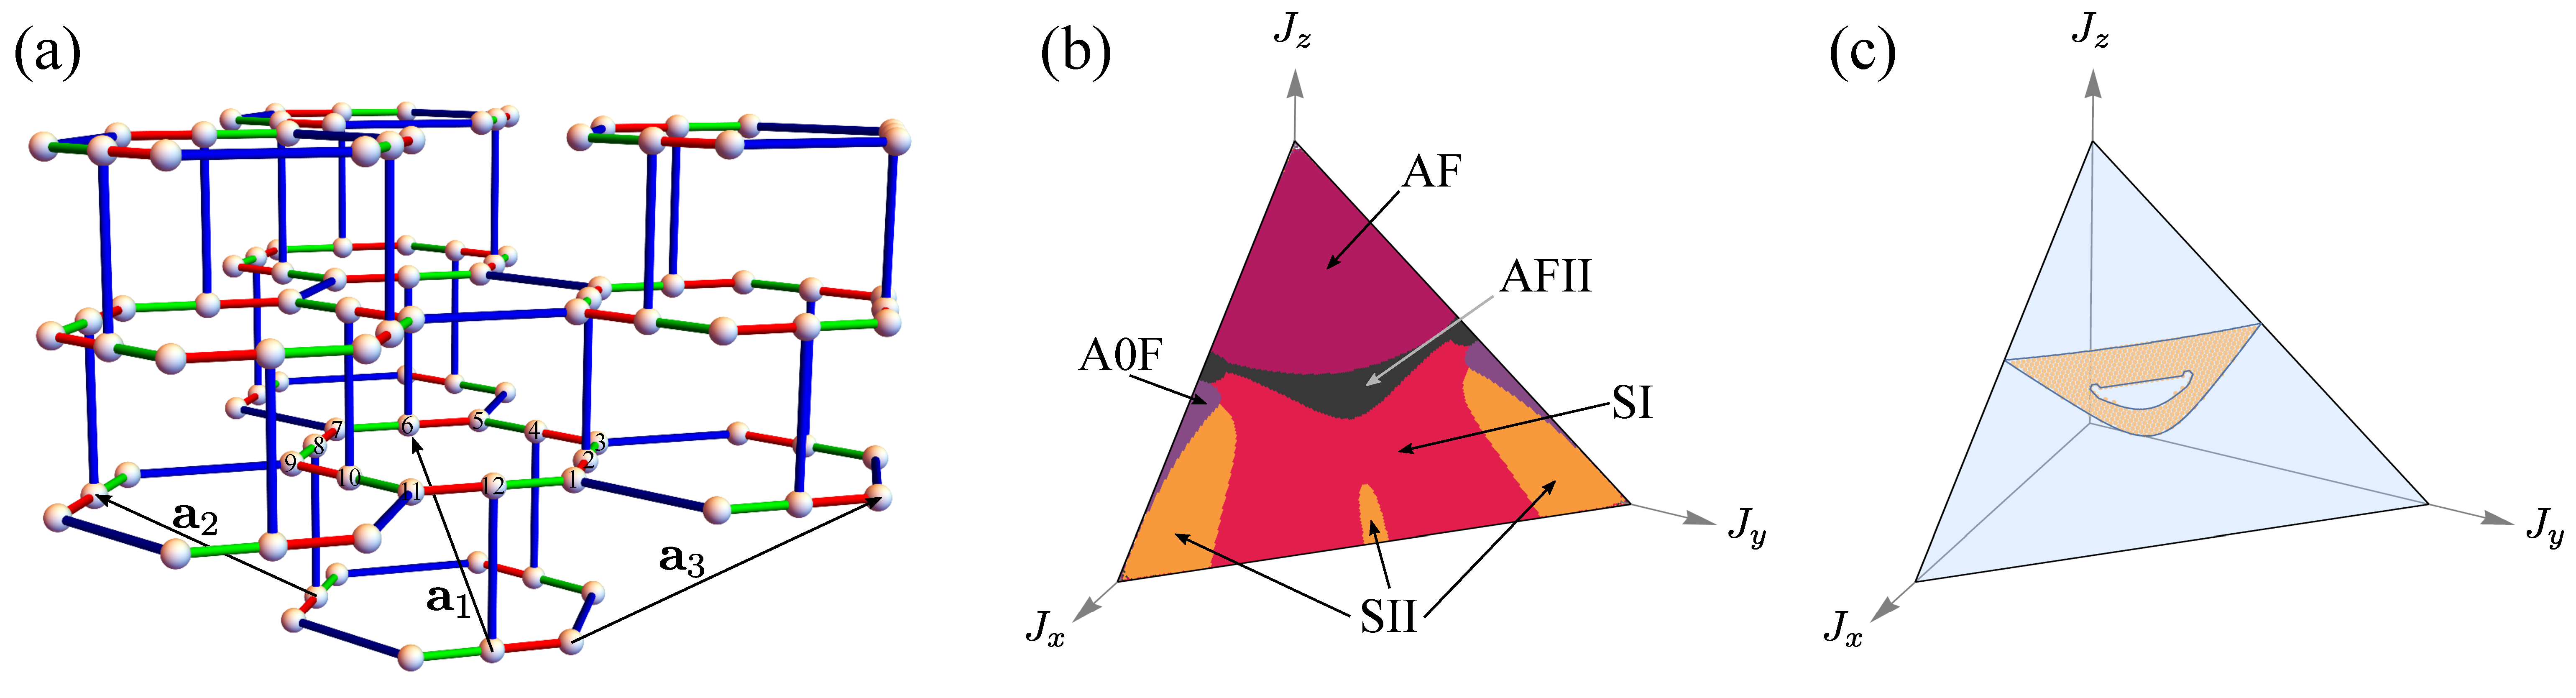
\includegraphics[width=\linewidth]{./chapter06/9_3aPanel.pdf}
	\caption{
		(a) Unit cell and translation vectors for the Kitaev model on the deformed version of lattice (9,3)a.
		(b) Ground state flux phase diagram for lattice (9,3)a.
		(c) Fermionic ground state phase diagram for lattice (9,3)a.
		The orange and blue shaded regions indicate the gapless and gapped spin liquid phases, respectively.
		The data points denoting these two phases were obtained from the corresponding Berry flux calculation.
		The phase boundary is a composite of Berry flux data and gap closing data, as described in the main text.
	}
	\label{fig:chapter06_9_3aPanel}
\end{figure}
%

The lattice is seen to possess a $C_3$ symmetry with rotation axis in the middle of the twelve-site unit cell pointing in the $\hat{e}_z$-direction.
There are three mirror planes which cut through the $z$-type bonds and act to map $x$- and $y$-type bonds onto one another by mapping $\ba_2 \leftrightarrow \ba_3$, $\ba_3 \leftrightarrow \ba_1$ or $\ba_1 \leftrightarrow \ba_2$.
Finally, the lattice is inversion symmetric with multiple, unique inversion centers.
All inversion symmetries map bonds of a given type to the same type of bond.
The first inversion center lies at the center of the twelve-site unit cell, whereas the others are located at the midpoint of the line connecting the aforementioned inversion centers from neighboring unit cells.


%
%
%%%%%%%%%%%%%%%%%%%%%%%%%%%%%%%%%%%%%%%%%%%%%%%%%%%%%%%%%%%%%%%%%%%%%%%%%%%%%%%%%%%%%%%%
\section{Ground state flux configurations}
\label{section:chapter06_Fluxes}
%%%%%%%%%%%%%%%%%%%%%%%%%%%%%%%%%%%%%%%%%%%%%%%%%%%%%%%%%%%%%%%%%%%%%%%%%%%%%%%%%%%%%%%%
%
%
%%%%%%%%%%%%%%%%%%%%%%%%%%%%%%%%%%%%%%%%%%%%%%%%%%%%%%%%%%%%%%%%%%%%%%%%%%%%%%%%%%%%%%%%
\subsection{Quantum Monte Carlo simulations}
\label{section:chapter06_QMC}
%%%%%%%%%%%%%%%%%%%%%%%%%%%%%%%%%%%%%%%%%%%%%%%%%%%%%%%%%%%%%%%%%%%%%%%%%%%%%%%%%%%%%%%%
%
%
As the quantum Monte Carlo (QMC) simulations of the Kitaev model for lattice (9,3)a were not performed by the author of this work, but rather by his collaborators P.~A. Mishchenko and Y. Kato, a detailed explanation of the methods used will not be provided here.
However, in order to frame the remainder of this work, this section will explain the basic ideas behind the simulations.

Due to the bond-dependent interactions of the Kitaev Hamiltonian
%
\begin{equation}
	\op{H}_{\rm Kitaev} = -J_x \sum_{x {\rm -links}} \sigma_j^x \sigma_k^x - J_y \sum_{y {\rm -links}} \sigma_j^y \sigma_k^y - J_z \sum_{z {\rm -links}} \sigma_j^z \sigma_k^z,
\end{equation}
%
the usual spin QMC methods based on the Suzuki-Trotter decomposition suffer from the negative sign problem and cannot be used~\cite{NasuPRL2014}.
However, in Chapter~\ref{chapter:KitaevHoneycombModel} it was seen that the Kitaev Hamiltonian may be reframed as a free Majorana Hamiltonian in the background of a static \ZZ~gauge field.
The fermionic Kitaev Hamiltonian in a fixed gauge sector may be straightforwardly diagonalized and the resulting eigenbasis used in the QMC simulations in order to avoid the sign problem~\cite{NasuPRL2014}.
In practice, rather than using the Majorana representations seen in Chapters~\ref{chapter:KitaevHoneycombModel} and~\ref{chapter:ProjectiveSymmetryGroup}, the model is solved via Jordan-Wigner transformation~\cite{ChenPRB2007,FengPRL2007,ChenJPA2008}, resulting in the free Majorana Hamiltonian
%
\begin{equation}
	\op{H}(\{\eta\}) = i J_x \sum_{x {\rm -links}} \eta_{jk} c_j c_k + i J_y \sum_{y {\rm -links}} c_j c_k + i J_z \sum_{z {\rm -links}} c_j c_k,
	\label{eq:chapter06_JWHamiltonian}
\end{equation}
%
where a convention for the orientation of bonds must be fixed and $\eta_{jk} = \pm 1$ is a \ZZ~degree of freedom living only on the $x$-type bonds.

The QMC simulation may now be performed by sampling the classical, Ising-like variables $\eta_{ij}$, where the Monte Carlo weight for a given configuration of $\{\eta\}$ is obtained by the exact diagonalization of the Majorana fermions in Hamiltonian~\eqref{eq:chapter06_JWHamiltonian}.
In practice, other numerical "tricks" are employed to access larger system sizes and lower temperatures.
For example, the simulations do not use exact diagonalization to determine the Monte Carlo weight of a given configuration of $\{\eta\}$, rather, they employ a kernel polynomial method~\cite{WeisseRMP2006,WeissePRL2009} to approximate the difference in free energy between two configurations, reducing the numerical cost from $\mathcal{O}(N^4)$ to $\mathcal{O}(N^2)$, where $N$ is the total number of spins~\cite{MischenkoPRB2017}.
Additionally, the simulations utilized feedback-optimized parallel tempering methods in order to access lower temperatures~\cite{TrebstPRE2004,KatzgraberJSM2006}.
\begin{figure}[tb]
	\centering
	\includegraphics[width=\linewidth]{./chapter06/9_3aFluxConfigurations.pdf}
	\caption{
		Flux configurations for lattice (9,3)a where the flux loops are represented by colored spheres.
		Loops of length 9 are colored white or black corresponding to $+\pi/2$-flux or $-\pi/2$-flux, respectively.
		Loops of length 12 are colored blue or red corresponding to $\pi$-flux or $0$-flux, respectively.
		(a) Single flux unit cell of lattice (9,3)a.
		(b) Flux configuration A0F.
		(c) Flux configuration SII.
		(d) Flux configuration SI.
		(e) Flux configuration AF.
		(f) Flux configuration AFII.
	}
	\label{fig:chapter06_9_3aFluxConfigurations}
\end{figure}
%


%
%
%%%%%%%%%%%%%%%%%%%%%%%%%%%%%%%%%%%%%%%%%%%%%%%%%%%%%%%%%%%%%%%%%%%%%%%%%%%%%%%%%%%%%%%%
\subsection{Results}
\label{section:chapter06_QMCResults}
%%%%%%%%%%%%%%%%%%%%%%%%%%%%%%%%%%%%%%%%%%%%%%%%%%%%%%%%%%%%%%%%%%%%%%%%%%%%%%%%%%%%%%%%
%
%
%
In addition to the QMC simulations described above, a number of potential ground state flux configurations were found from effective models obtained in the various limits of anisotropic exchange couplings via perturbation theory.
A combination of the QMC results along with a straightforward variational approach using the aforementioned trial flux configurations was used to determine the ground state flux configuration as a function of exchange couplings.
The resulting ground state flux phase diagram is pictured in Figure~\ref{fig:chapter06_9_3aPanel}~(b).
As can be seen from the figure, the ground state of the Kitaev model on lattice (9,3)a exhibits a variety of different flux phases.
It turns out that the SII and A0F flux phases (depicted in Figures~\ref{fig:chapter06_9_3aFluxConfigurations}~(b) and (c), respectively) correspond to fully gapped quantum spin liquid ground states, whereas the SI, AF and AFII flux phases (depicted in Figures~\ref{fig:chapter06_9_3aFluxConfigurations}~(d), (e) and (f), respectively) host both gapped and gapless quantum spin liquid ground states depending on the exact choice of coupling strengths.
The distinction lies in the gapped/gapless nature of the fermionic quasiparticle excitations which are explored in detail in the remainder of this chapter.


%
%
%%%%%%%%%%%%%%%%%%%%%%%%%%%%%%%%%%%%%%%%%%%%%%%%%%%%%%%%%%%%%%%%%%%%%%%%%%%%%%%%%%%%%%%%
\section{Gapless spin liquids}
\label{section:chapter06_GaplessSpinLiquids}
%%%%%%%%%%%%%%%%%%%%%%%%%%%%%%%%%%%%%%%%%%%%%%%%%%%%%%%%%%%%%%%%%%%%%%%%%%%%%%%%%%%%%%%%
%
%
%%%%%%%%%%%%%%%%%%%%%%%%%%%%%%%%%%%%%%%%%%%%%%%%%%%%%%%%%%%%%%%%%%%%%%%%%%%%%%%%%%%%%%%%
\subsection{Fermionic phase diagram}
\label{section:chapter06_GaplessPhaseDiagram}
%%%%%%%%%%%%%%%%%%%%%%%%%%%%%%%%%%%%%%%%%%%%%%%%%%%%%%%%%%%%%%%%%%%%%%%%%%%%%%%%%%%%%%%%
%
%
Given the ground state \textit{flux} phase diagram discussed in Section~\ref{section:chapter06_Fluxes}, the \textit{fermionic} ground state phase diagram may be mapped out by assigning the correct flux configuration for a given choice of exchange couplings and checking the resulting fermionic spectrum.
In order to efficiently determine whether the fermionic quasiparticles are gapped or gapless at a given point in the phase diagram, the non-Abelian Berry curvature is integrated over two-dimensional planes which cut through the three-dimensional Brillouin zone, \ie, by fixing one component of the momentum and integrating over the other two~\cite{FukuiJPS2005}.
This is analogous to what was described in Section~\ref{section:chapter05_8_3b} to calculate the chirality of Weyl nodes.

For those planes on which the fermionic spectrum is gapped, the result is a quantized Chern number.
In a Weyl spin liquid phase, the Chern number jumps discontinuously as the plane passes through a Weyl node by an amount equal to the charge of that Weyl node.
In general, the Berry curvature is ill-defined for a plane on which the fermionic spectrum is gapless.
In the case that there is a one- or two-dimensional nodal manifold, the result is a range of momentum values for which the Berry flux is ill-defined and fluctuates wildly.

With this information, it may be determined whether a given point in the phase diagram corresponds to a gapped or gapless fermionic spectrum.
If the Berry flux is everywhere vanishing, the fermions must be gapped throughout the entire Brillouin zone.
However, if at any point the Berry flux is \textit{non-zero} -- whether it takes a non-vanishing quantized Chern number or fluctuates wildly -- the fermionic spectral gap must close somewhere.
For those regions of the phase diagram where the gap closing occurs at a high-symmetry point, the resolution of the phase diagram data was greatly increased by checking whether or not the gap closes at that point for a given choice of couplings. 
The resulting fermionic ground state phase diagram is pictured in  Figure~\ref{fig:chapter06_9_3aPanel}~(c).

In Figure~\ref{fig:chapter06_9_3aPanel}, the ground state phase diagrams for the \ZZ~gauge field and the fermions are pictured separately for clarity.
Composites of the two phase diagrams appear below, however, in the context of the different gapless spin liquid phases.
Whereas the flux phases A0F and SII are seen to be fully gapped, the flux phases SI, AF and AFII have both gapped and gapless regions.
In the following sections, the nature of the gapless regions are discussed for the flux phases SI, AF and AFII.
In all cases, the elementary unit cell is doubled in all directions to accommodate the gauge \textit{Ansatz}.


%
%
%%%%%%%%%%%%%%%%%%%%%%%%%%%%%%%%%%%%%%%%%%%%%%%%%%%%%%%%%%%%%%%%%%%%%%%%%%%%%%%%%%%%%%%%
\subsection{SI flux phase}
\label{section:chapter06_SIPhase}
%%%%%%%%%%%%%%%%%%%%%%%%%%%%%%%%%%%%%%%%%%%%%%%%%%%%%%%%%%%%%%%%%%%%%%%%%%%%%%%%%%%%%%%%
%
%
\subsubsection{Gauge structure and projective symmetries}
%
%
In the SI flux configuration, all loops of length 12 are assigned $\pi$-flux, whereas the loops of length 9 are assigned $\pm \pi/2$-flux according to their position in the unit cell.
A representation of the SI flux configuration is pictured in Figure~\ref{fig:chapter06_9_3aFluxConfigurations}~(d).
Although the flux configuration has the same translation symmetry as the lattice, the unit cell is doubled in all directions to accommodate the gauge \textit{Ansatz}.

The arrangement of fluxes is seen to respect inversion symmetry for \textit{all} inversion centers, however, it breaks $C_3$ symmetry and two out of three mirror symmetries.
By virtue of lattice (9,3)a being non-bipartite, the flux configuration necessarily breaks time-reversal symmetry (see Section~\ref{section:chapter05_9_3a} for details).

The projective symmetry operators have not been explicitly constructed due to the enormous 96 site unit cell, however, the fermionic spectrum is seen \textit{not} to possess any finite nesting vectors.
The relevant energy relations are, thus, given by
%
\begin{equation}
	E_{\alpha}(\bk) = -E_{\beta}(-\bk) \qquad {\rm and} \qquad E_{\alpha}(\bk) = E_{\gamma}(-\bk),
\end{equation}
%
due to particle-hole and inversion symmetry, respectively.
Due to the lack of a projective time-reversal operator, the momentum space Hamiltonian matrix has the general form
%
\begin{equation}
	H(\bk) = 
		\begin{pmatrix}
			0			&		 & A(\bk) \\
						& \ddots & 		  \\
			A\dag(\bk)	&		 & 0
		\end{pmatrix},
\end{equation}
%
\ie, it is an inversion symmetric band Hamiltonian.


%
%
\subsubsection{Majorana band structure}
%
%
%
\begin{figure}[tb]
	\centering
	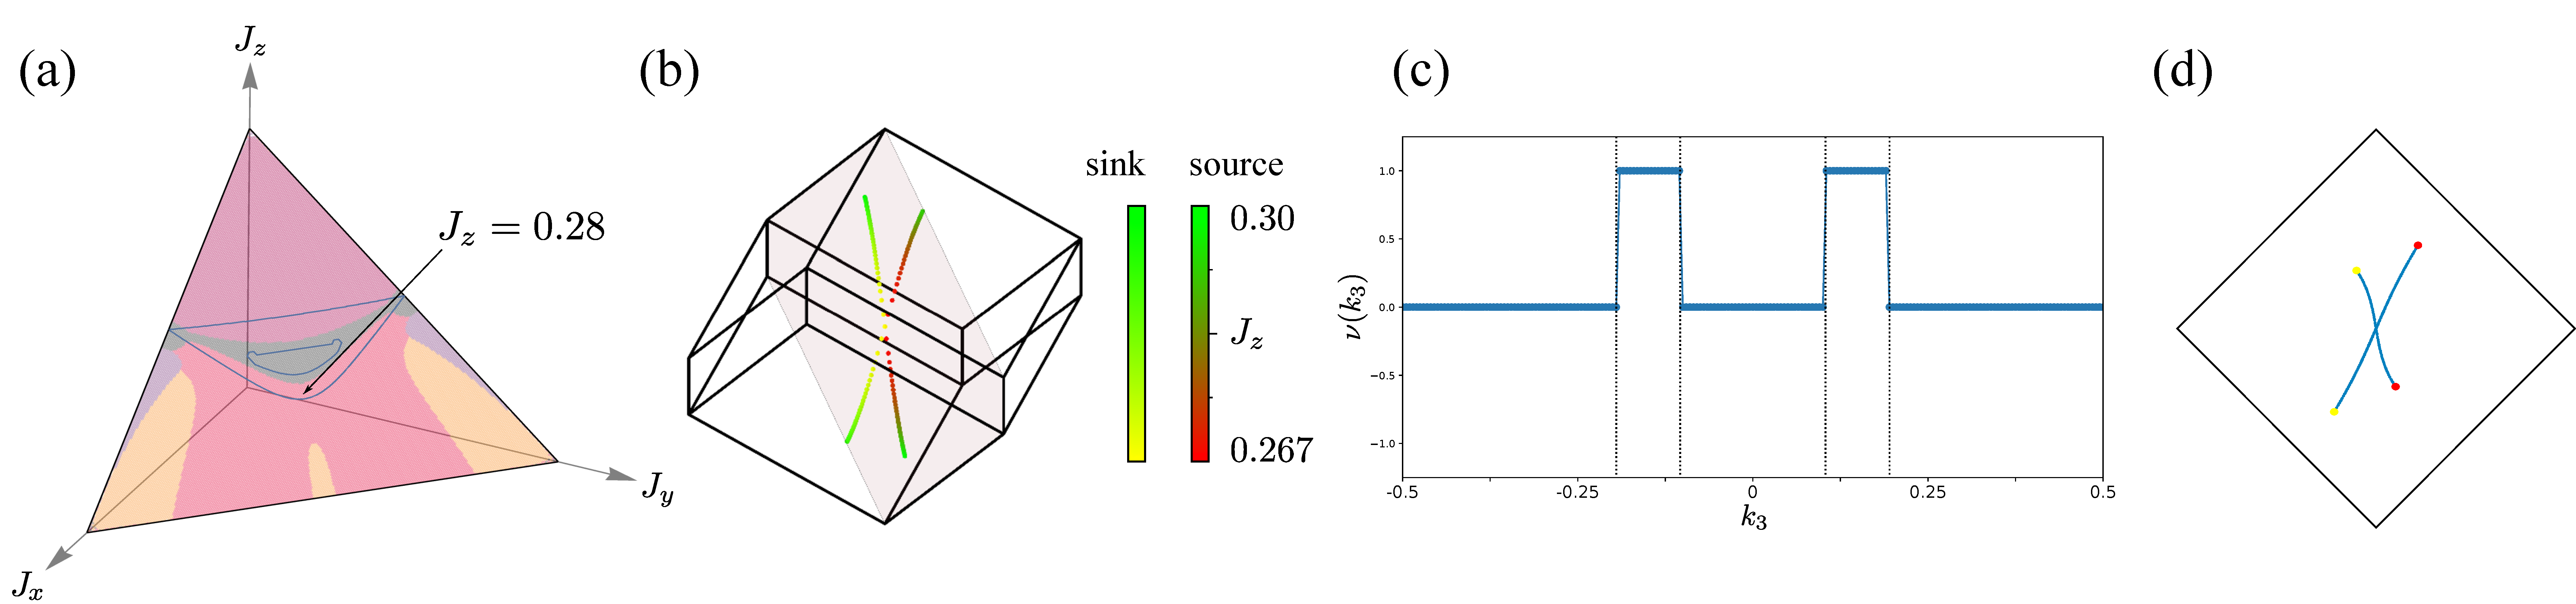
\includegraphics[width=\linewidth]{./chapter06/9_3a_SIPanel.pdf}
	\caption{
		(a) Gapless SI phase for lattice (9,3)a.
		The arrow indicates the point $(J_x, J_y, J_z) = (0.36, 0.36, 0.28)$.
		For fixed $J_x = J_y = (1 - J_z)/2$, the gapless portion of the SI phase begins for $J_z \gtrsim 0.267$ where the gap closes and ends for $J_z \gtrsim 0.3$ where the ground state flux configuration switches from SI to AFII.
		(b) Evolution of Weyl nodes for lattice (9,3)a for varied coupling constants $0.267 \leq J_z \leq 0.30$ with $J_x = J_y = (1 - J_z)/2$.
		The shaded region indicates the remaining mirror plane for the SI flux phase with $J_x = J_y$.
		(c) Chern number as a function of momentum $k_3$ for the choice of couplings $(J_x, J_y, J_z) = (0.36, 0.36, 0.28)$.
		The dashed lines indicate the $k_3$-component of the Weyl node positions.
		(d) Corresponding Fermi arcs in the 001-surface Brillouin zone for $(J_x, J_y, J_z) = (0.36, 0.36, 0.28)$.
	}
	\label{fig:chapter06_SIPanel}
\end{figure}
%
As discussed in Chapter~\ref{chapter:ClassificationOfKSL}, the presence of trivially implemented inversion symmetries, \ie, with vanishing nesting vector, prohibits the formation of stable Fermi surfaces.
Furthermore, the absence of time-reversal symmetry prevents the formation of nodal lines protected by the one-dimensional winding number discussed in Section~\ref{section:chapter05_8_3c}.
However, the combination of particle-hole and inversion symmetries allows for the presence of topologically protected Weyl nodes pinned to zero energy.

Indeed, diagonalizing the concrete Hamiltonian for lattice (9,3)a in the SI flux configuration reveals an extended gapless Weyl spin liquid phase (see Figure~\ref{fig:chapter06_SIPanel}~(a)).
Restricting the exchange couplings to the line $J_x = J_y = (1 - J_z)/2$, the gapless portion of the SI phase runs from $J_z \approx 0.267$, where the gap closes, to $J_z \approx 0.3$, where the ground state flux configuration switches from SI to AFII.
For $J_z \approx 0.267$, two positively charged and two negatively charged Weyl nodes simultaneously appear at the $\Gamma$-point.
As $J_z$ is increased further, the Weyl nodes split apart.
For $J_x = J_y$, the Weyl nodes are pinned to the single mirror plane which is \textit{not} broken by the SI flux configuration.

Figure~\ref{fig:chapter06_SIPanel}~(b) shows the evolution of the Weyl nodes in the 3D Brillouin zone as the exchange couplings are varied for $0.276 \leq J_z \leq 0.30$ with $J_x = J_y = (1 - J_z)/2$, along with the aforementioned mirror plane.
The trajectory of negatively charged Weyl nodes changes color from yellow to green as $J_z$ is increased, whereas the trajectory of positively charged Weyl nodes changes from red to green.
In Figure~\ref{fig:chapter06_SIPanel}~(c) is plotted the Chern number as a function of $k_3 = \bk \cdot \bq_3 / 2\pi$ for $(J_x, J_y, J_z) = (0.36, 0.36, 0.28)$, indicating the charge of the Weyl nodes in the bulk.
The corresponding Fermi arcs in the 001-surface Brillouin zone for the same choice of couplings are plotted in Figure~\ref{fig:chapter06_SIPanel}~(d).


%
%
%%%%%%%%%%%%%%%%%%%%%%%%%%%%%%%%%%%%%%%%%%%%%%%%%%%%%%%%%%%%%%%%%%%%%%%%%%%%%%%%%%%%%%%%
\subsection{AF flux phase}
\label{section:chapter06_AFPhase}
%%%%%%%%%%%%%%%%%%%%%%%%%%%%%%%%%%%%%%%%%%%%%%%%%%%%%%%%%%%%%%%%%%%%%%%%%%%%%%%%%%%%%%%%
%
%
\subsubsection{Gauge structure and projective symmetries}
%
%
In the AF flux configuration, all loops of length 12 are assigned $\pi$-flux, whereas the loops of length 9 are assigned $\pm \pi/2$-flux according to their position in the unit cell.
A representation of the AF flux configuration is pictured in Figure~\ref{fig:chapter06_9_3aFluxConfigurations}~(e).
Although the flux configuration has the same translation symmetry as the lattice, the unit cell is doubled in all directions to accommodate the gauge \textit{Ansatz}.

The arrangement of fluxes is seen to respect inversion symmetry for \textit{all} inversion centers, as well as the $C_3$-rotation symmetry and all mirror symmetries.
By virtue of lattice (9,3)a being non-bipartite, the flux configuration necessarily breaks time-reversal symmetry (see Section~\ref{section:chapter05_9_3a} for details).

The projective symmetry operators have not been explicitly constructed due to the enormous 96 site unit cell, however, the fermionic spectrum is seen \textit{not} to possess any finite nesting vectors.
The relevant energy relations are, thus, given by
%
\begin{equation}
	E_{\alpha}(\bk) = -E_{\beta}(-\bk) \qquad {\rm and} \qquad E_{\alpha}(\bk) = E_{\gamma}(-\bk),
\end{equation}
%
due to particle-hole and inversion symmetry, respectively.
Due to the lack of a projective time-reversal operator, the momentum space Hamiltonian matrix has the general form
%
\begin{equation}
	H(\bk) = 
		\begin{pmatrix}
			0			&		 & A(\bk) \\
			& \ddots & 		  \\
			A\dag(\bk)	&		 & 0
		\end{pmatrix},
\end{equation}
%
\ie, it is an inversion symmetric band Hamiltonian.


%
%
\subsubsection{Majorana band structure}
%
%
%
\begin{figure}[tb]
	\centering
	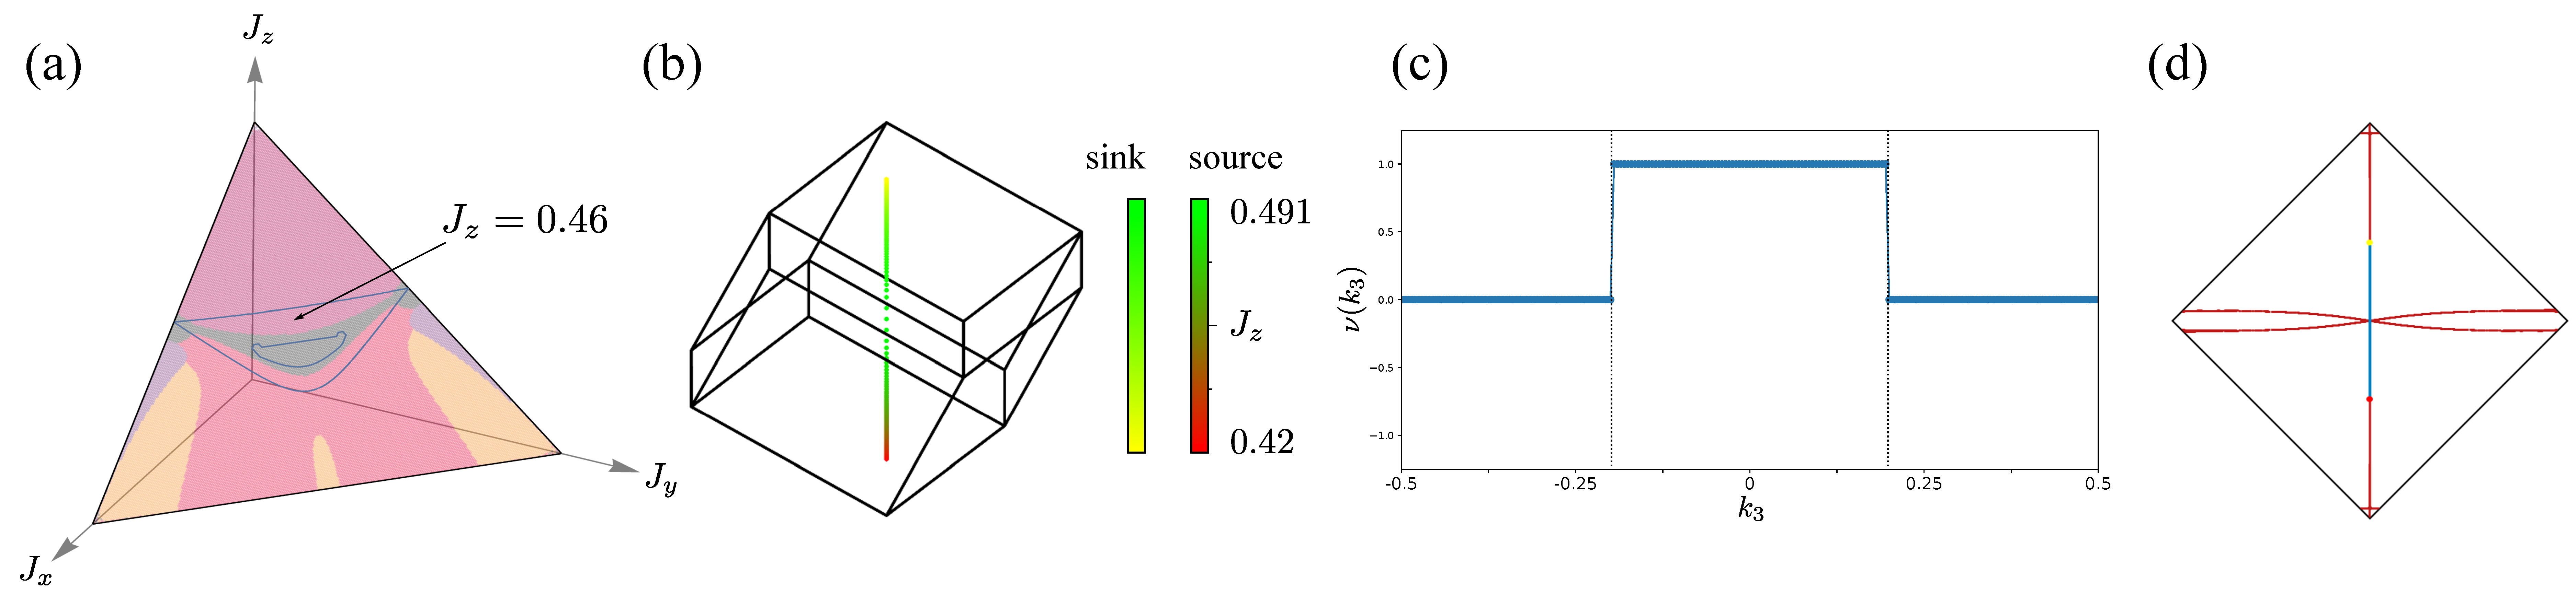
\includegraphics[width=\linewidth]{./chapter06/9_3a_AFPanel.pdf}
	\caption{
		(a) Gapless AF phase for lattice (9,3)a.
		The arrow indicates the point $(J_x, J_y, J_z) = (0.27, 0.27, 0.46)$.
		For fixed $J_x = J_y = (1 - J_z)/2$, the gapless portion of the AF phase begins for $J_z \gtrsim 0.42$, where the ground state flux configuration switches from AFII to AF, and ends for $J_z \gtrsim 0.491$, where the gap reopens.
		(b) Evolution of Weyl nodes for lattice (9,3)a for varied coupling constants $0.42 \leq J_z \leq 0.491$ with $J_x = J_y = (1 - J_z)/2$.
		(c) Chern number as a function of momentum $k_3$ for the choice of couplings $(J_x, J_y, J_z) = (0.27, 0.27, 0.46)$.
		The dashed lines indicate the $k_3$-component of the Weyl node positions.
		(d) Corresponding Fermi arc in the 001-surface Brillouin zone for $(J_x, J_y, J_z) = (0.27, 0.27, 0.46)$ denoted in blue.
		Additional surface states are marked in red and are discussed in the main text.
	}
	\label{fig:chapter06_AFPanel}
\end{figure}
%
As is the case for the SI phase discussed above, the presence of trivially implemented inversion symmetries, \ie, with vanishing nesting vector, prohibits the formation of stable Fermi surfaces.
Furthermore, the absence of time-reversal symmetry prevents the formation of nodal lines protected by the one-dimensional winding number discussed in Section~\ref{section:chapter05_8_3c}.
However, the combination of particle-hole and inversion symmetries allows for the presence of topologically protected Weyl nodes pinned to zero energy.
%
\begin{figure}[tb]
	\centering
	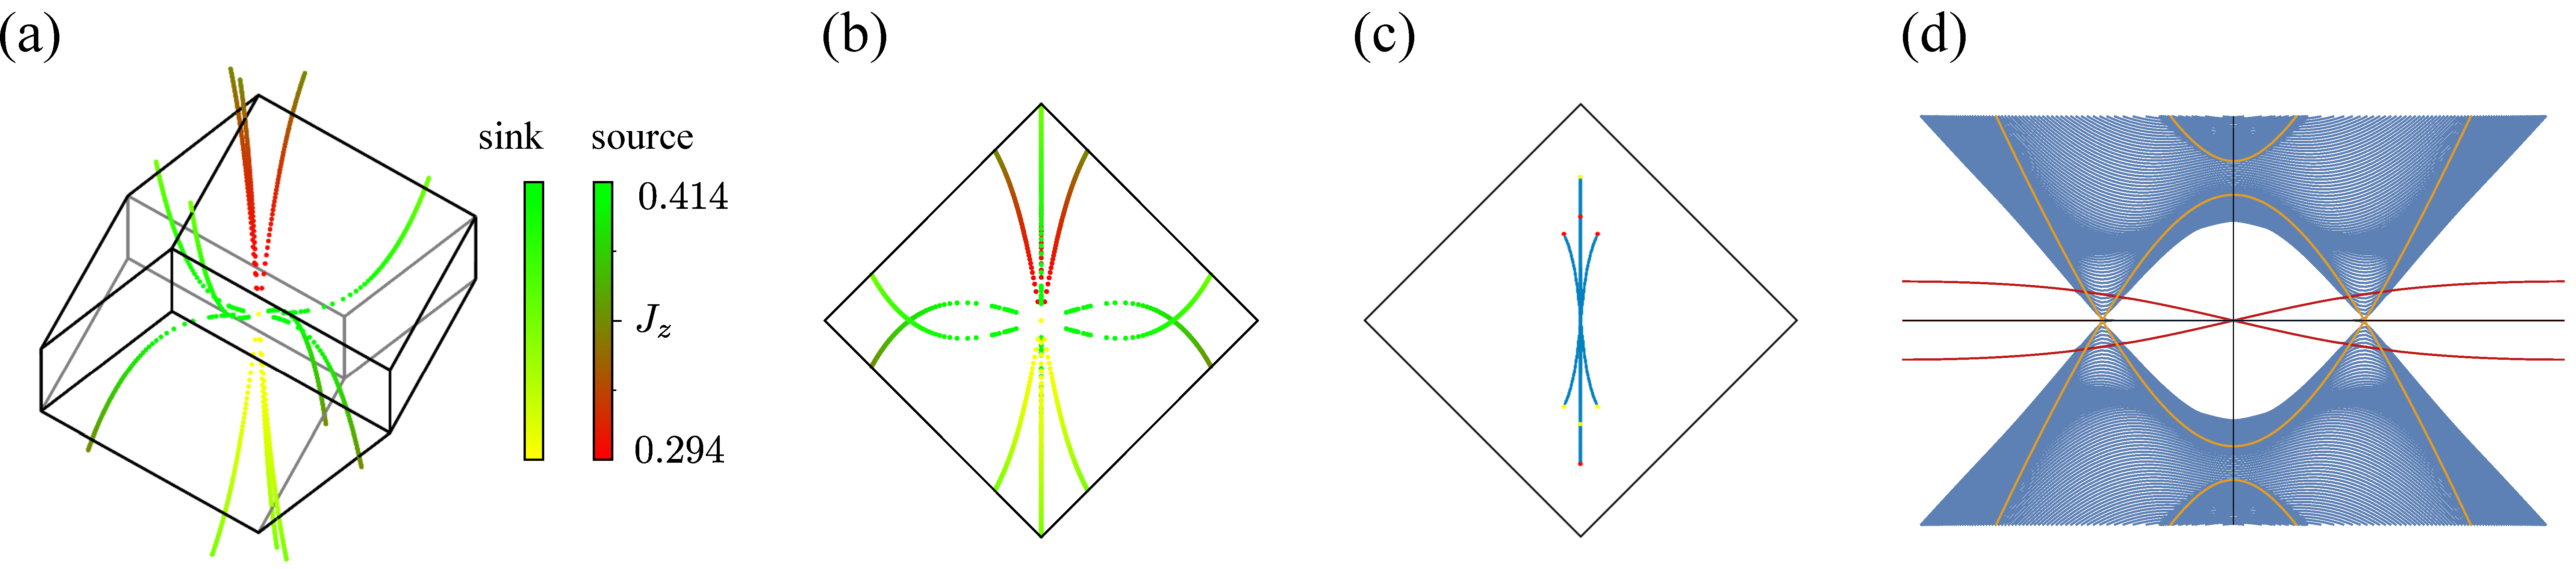
\includegraphics[width=\linewidth]{./chapter06/9_3a_AFPanel2.pdf}
	\caption{
		(a) Evolution of Weyl nodes for lattice (9,3)a for varied coupling constants $0.294 \leq J_z \leq 0.414$ with $J_x = J_y = (1 - J_z)/2$.
		The two Weyl nodes on the $C_3$-invariant axis are not shown for clarity.
		(b) Evolution of Weyl nodes for lattice (9,3)a for varied coupling constants $0.294 \leq J_z \leq 0.414$ with $J_x = J_y = (1 - J_z)/2$ projected down to the 001-surface Brillouin zone.
		The two Weyl nodes on the $C_3$-invariant axis are not shown for clarity.
		(c) Corresponding Fermi arcs in the 001-surface Brillouin zone for $(J_x, J_y, J_z) = (0.345, 0.345, 0.31)$.
		This includes the Weyl nodes which lie on the $C_3$-invariant axis along with their corresponding Fermi arc.
		(d) Band structures for $J_z = 0.46$.
		The bulk band structure along the $C_3$-invariant axis is plotted in yellow showing the two Weyl nodes.
		The band structure for the slab geometry along the projection of the $C_3$ axis to the surface Brillouin zone is plotted in blue and red.
		Here in blue are seen the projection of the two Weyl nodes as well as the Fermi arc which connects them.
		In red are plotted the bands responsible for the remaining surface states left over from the other Weyl nodes which are gapped out for $J_z \approx 0.414$.
	}
	\label{fig:chapter06_AFPanel2}
\end{figure}
%

Indeed, diagonalizing the concrete Hamiltonian for lattice (9,3)a in the AF flux configuration reveals an extended gapless Weyl spin liquid phase (see Figure~\ref{fig:chapter06_AFPanel}~(a)).
Restricting the exchange couplings to the line $J_x = J_y = (1 - J_z)/2$, the gapless portion of the AF phase runs from $J_z \approx 0.42$, where the ground state flux configuration switches from AFII to AF, to $J_z \approx 0.491$, where the Weyl nodes gap out.
For $0.42 < J_z \lesssim 0.491$, two oppositely charged Weyl nodes are pinned to the $C_3$-invariant axis while $J_x = J_y$.
As $J_z$ is increased, the two Weyl nodes move towards each other until they eventually meet at the $\Gamma$-point for $J_z \approx 0.491$ and mutually annihilate.

Figure~\ref{fig:chapter06_AFPanel}~(b) shows the evolution of the Weyl nodes in the 3D Brillouin zone as the exchange couplings are varied for $0.42 \leq J_z \leq 0.491$ with $J_x = J_y = (1 - J_z)/2$.
The trajectory of negatively charged Weyl nodes changes color from yellow to green as $J_z$ is increased, whereas the trajectory of positively charged Weyl nodes changes from red to green.
In Figure~\ref{fig:chapter06_AFPanel}~(c) is plotted the Chern number as a function of $k_3 = \bk \cdot \bq_3 / 2\pi$ for $(J_x, J_y, J_z) = (0.27, 0.27, 0.46)$, indicating the charge of the Weyl nodes in the bulk.
The corresponding Fermi arc in the 001-surface Brillouin zone for the same choice of couplings are plotted in Figure~\ref{fig:chapter06_AFPanel}~(d).

In addition to the Fermi arc which terminates at the projection of the Weyl nodes in the surface Brillouin zone, there appear additional line-like surface states which form incontractible loops.
These can be seen as remnants of Fermi arcs due to Weyl nodes which are gapped out in this part of the phase diagram.
If the AF flux configuration is extended beyond its range of validity, \ie, for $J_z \lesssim 0.42$ with $J_x = J_y$, one finds the existence of an additional six Weyl nodes.
These Weyl nodes emerge from the $\Gamma$-point at $J_z \approx 0.294$ and move away from one another as $J_z$ is increased, always pinned to the three mirror planes.
At $J_z \approx 0.414$, the six Weyl nodes once again meet and annihilate at the $\Gamma$-point.
However, as they do so, they trace out incontractible loops across the Brillouin zone.
In Figure~\ref{fig:chapter06_AFPanel2}~(a) and (b) are pictured the evolution of these six additional Weyl nodes (excluding the two Weyl nodes on the $C_3$-invariant axis mentioned in the previous paragraph) in the bulk Brillouin zone and projected down to the 001-surface Brillouin zone, respectively.
Here can be seen the incontractible loops along which they travel before gapping out.

A consequence of their trajectories through the Brillouin zone is that their corresponding Fermi arcs (pictured in Figure~\ref{fig:chapter06_AFPanel2}~(c)), rather than shrinking to a point and gapping out with the Weyl nodes, are stretched out along similar incontractible loops.
The result is that, while the Weyl nodes responsible for the surface states gap out, the surface states themselves remain behind (as can be seen in Figure~\ref{fig:chapter06_AFPanel}~(d) pictured in red).
Pictured in Figure~\ref{fig:chapter06_AFPanel2}~(d) is a composite of the bulk and slab geometry band structures for $J_z = 0.46$ computed along the $C_3$-invariant axis and its projection to the 001-surface Brillouin zone, respectively.
Here can be seen the Fermi arcs in blue which terminate at the projection of the Weyl nodes to the surface Brillouin zone at which point they dive back into the bulk.
In red, however, are pictured the remnant surface bands from the Weyl nodes which have been gapped out.
These bands are seen to be entirely disconnected from the bulk band structure.


%
%
%%%%%%%%%%%%%%%%%%%%%%%%%%%%%%%%%%%%%%%%%%%%%%%%%%%%%%%%%%%%%%%%%%%%%%%%%%%%%%%%%%%%%%%%
\subsection{AFII flux phase}
\label{section:chapter06_AFIIPhase}
%%%%%%%%%%%%%%%%%%%%%%%%%%%%%%%%%%%%%%%%%%%%%%%%%%%%%%%%%%%%%%%%%%%%%%%%%%%%%%%%%%%%%%%%
%
%
\subsubsection{Gauge structure and projective symmetries}
%
%
In the AFII flux configuration, all loops of length 12 are assigned $\pi$-flux, whereas the loops of length 9 are assigned $\pm \pi/2$-flux according to their position in the unit cell.
A representation of the AFII flux configuration is pictured in Figure~\ref{fig:chapter06_9_3aFluxConfigurations}~(f).
The AFII flux configuration requires a doubling of the unit cell in all directions.

The arrangement of fluxes is seen to respect $C_3$-rotation symmetry, all mirror symmetries and inversion symmetry through the point at the center of the unit cell, however, it breaks all other inversion symmetries.
By virtue of lattice (9,3)a being non-bipartite, the flux configuration necessarily breaks time-reversal symmetry (see Section~\ref{section:chapter05_9_3a} for details).
Note, however, that the combination of broken time-reversal with the broken inversion symmetry is indeed a symmetry of the AFII flux configuration.

The projective symmetry operators have not been explicitly constructed due to the enormous 96 site unit cell, however, the fermionic spectrum is seen \textit{not} to possess any finite nesting vectors.
The relevant energy relations are, thus, given by
%
\begin{equation}
	E_{\alpha}(\bk) = -E_{\beta}(-\bk) \qquad {\rm and} \qquad E_{\alpha}(\bk) = E_{\gamma}(-\bk),
\end{equation}
%
due to particle-hole and inversion symmetry, respectively.
Due to the lack of a projective time-reversal operator, the momentum space Hamiltonian matrix has the general form
%
\begin{equation}
	H(\bk) = 
		\begin{pmatrix}
			0			&		 & A(\bk) \\
			& \ddots & 		  \\
			A\dag(\bk)	&		 & 0
		\end{pmatrix},
\end{equation}
%
\ie, it is an inversion symmetric band Hamiltonian.


%
%
\subsubsection{Majorana band structure}
%
%
%
\begin{figure}[tb]
	\centering
	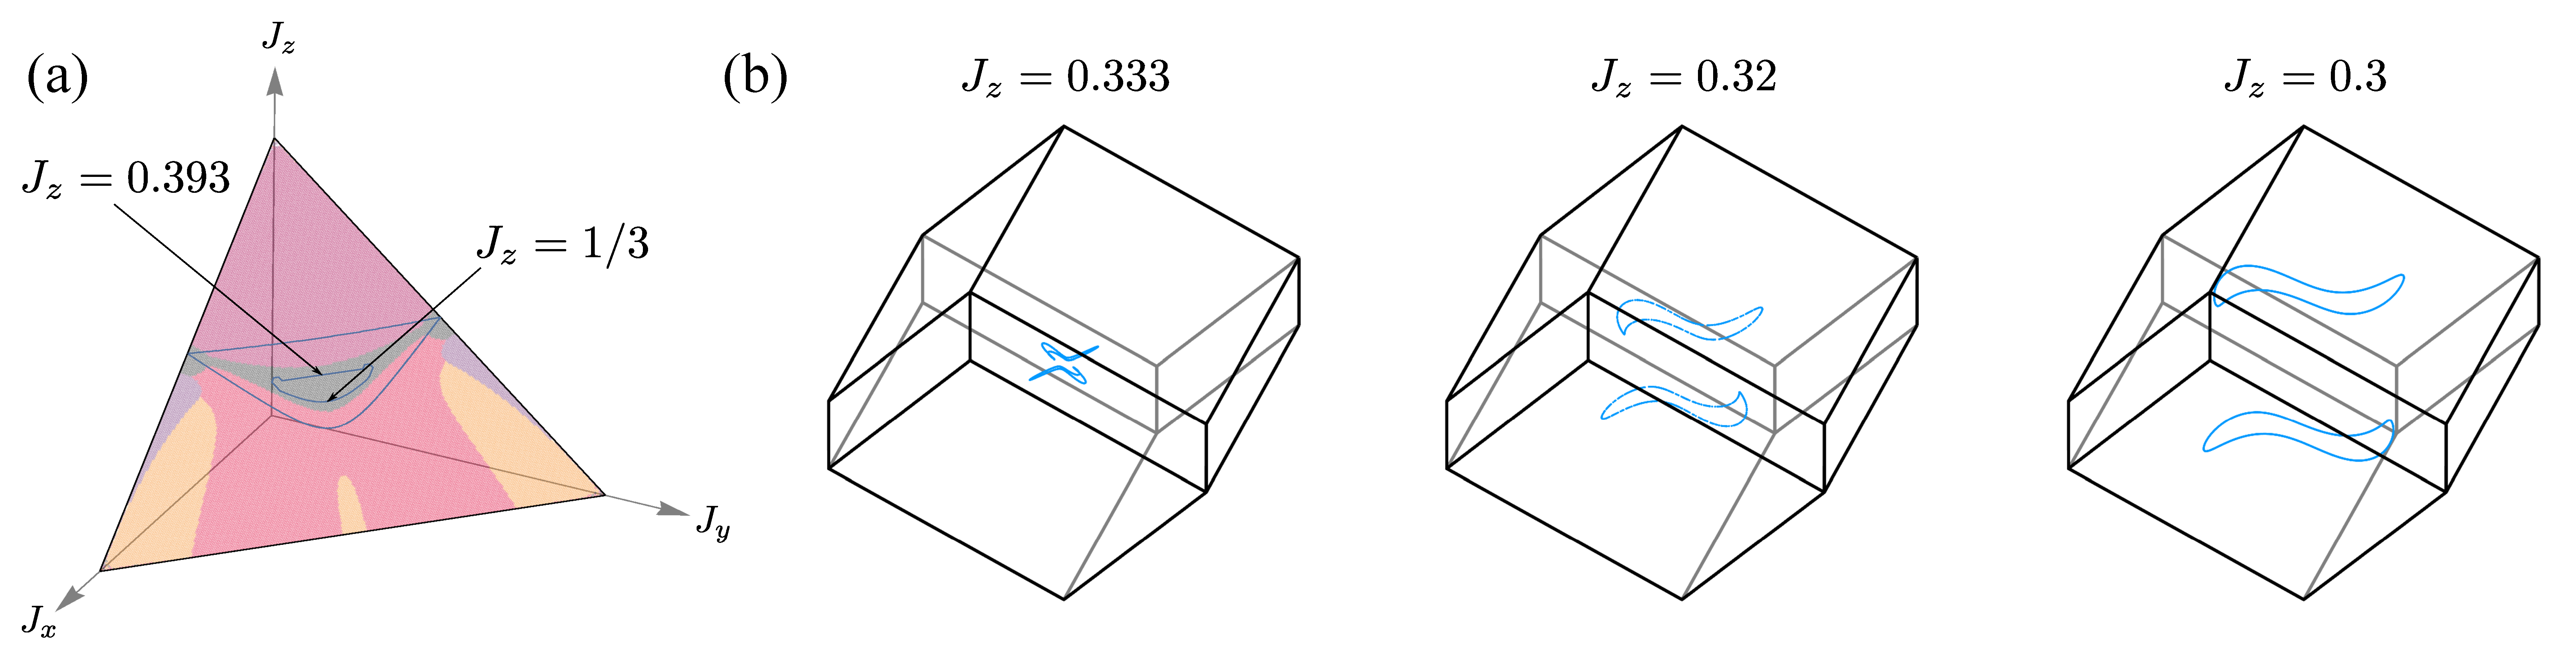
\includegraphics[width=\linewidth]{./chapter06/9_3a_AFIIPanel1.pdf}
	\caption{
		(a) Gapless AF phase for lattice (9,3)a.
		The arrows indicates the points $(J_x, J_y, J_z) = (1/3, 1/3, 1/3)$ and $(J_x, J_y, J_z) \approx (0.304, 0.304, 0.393)$.
		For fixed $J_x = J_y = (1 - J_z)/2$, the gapless portion of the AFII phase runs from $J_z \approx 0.3$, where the ground state flux configuration switches from SI to AFII, to $J_z \approx 0.42$, where the  ground state flux configuration switches from AFII to AF, with a region in between $1/3 < J_z \lesssim 0.392$ for which the spectrum is fully gapped.
		(b) Evolution of nodal lines for several values of $J_z < 1/3$.
	}
	\label{fig:chapter06_AFIIPanel}
\end{figure}
%
As already discussed above, the presence of trivially implemented inversion symmetry, \ie, with vanishing nesting vector, prohibits the formation of stable Fermi surfaces.
Furthermore, the absence of time-reversal symmetry prevents the formation of nodal lines protected by the one-dimensional winding number discussed in Section~\ref{section:chapter05_8_3c}.
%
%
%
However, it has been shown that in a system where the combination of inversion and time-reversal is a symmetry, one may define both one- and two-dimensional \ZZ~winding numbers~\cite{KimPRL2015,FangPRB2015}.
The one-dimensional winding number corresponds to a Berry phase of either 0 or $\pi$ acquired upon traversal of a one-dimensional loop and may stabilize nodal lines similarly to what was seen above for the time-reversal invariant spin liquids.
Additionally, pairs of nodal lines can be stabilized by the presence of a \textit{two}-dimensional \ZZ~winding number, \ie, a nodal line may carry a \ZZ~monopole charge defined on a two-dimensional surface which encloses it.
Due to their monopole charge, such nodal lines must always be created and annihilated in pairs rather than being continuously deformed to a point and gapped out in isolation.
Crucially, inversion and time-reversal operations need not individually be symmetries of the system, rather, only the combination of the two.
For lattice (9,3)a, any fixed flux sector breaks time-reversal symmetry spontaneously, however, in the AFII phase where one of the inversion symmetries is broken, the combination of the corresponding inversion operation with time-reversal indeed yields a symmetry of the Hamiltonian.
In this case, such line nodes can be stable.

Diagonalizing the concrete Hamiltonian for lattice (9,3)a in the AFII flux configuration reveals an extended gapless spin liquid phase with gapless excitations corresponding to nodal lines (see Figure~\ref{fig:chapter06_AFIIPanel}~(a)).
Restricting the exchange couplings to the line $J_x = J_y = (1 - J_z)/2$, the gapless portion of the AFII phase runs from $J_z \approx 0.3$, where the ground state flux configuration switches from SI to AFII, to $J_z \approx 0.42$, where the  ground state flux configuration switches from AFII to AF, with a region in between $1/3 < J_z \lesssim 0.392$ for which the spectrum is fully gapped.

At the isotropic point $J_z = 1/3$ there is a fourfold zero energy degeneracy at the $\Gamma$-point which is gapped out as soon as $J_z$ is increased.
However, for $J_z < 1/3$, this fourfold degeneracy is split into two nodal lines which grow larger and move away from each other as $J_z$ is increased further (see Figure~\ref{fig:chapter06_AFIIPanel}~(b)).
Extending the analysis of the AFII flux configuration for $J_z \lesssim 0.3$ where there is a phase transition to the SI flux phase, the nodal lines can be seen to wrap around the Brillouin zone before meeting once more and mutually annihilating at $J_z \approx 0.22$.
Putting the system on a slab geometry, one finds both "drumhead" surface states filling the projection of the nodal lines to the surface Brillouin zone~\cite{ChenNatComm2015,MullenPRL2015} as well as Fermi arc surface states connecting the two projections (see Figure~\ref{fig:chapter06_AFIIPanel3}~(a)) as a result of the \ZZ~monopole charges of the nodal lines~\cite{GorbarPRB2015a,GorbarPRB2015b}.
%
\begin{figure}[tb]
	\centering
	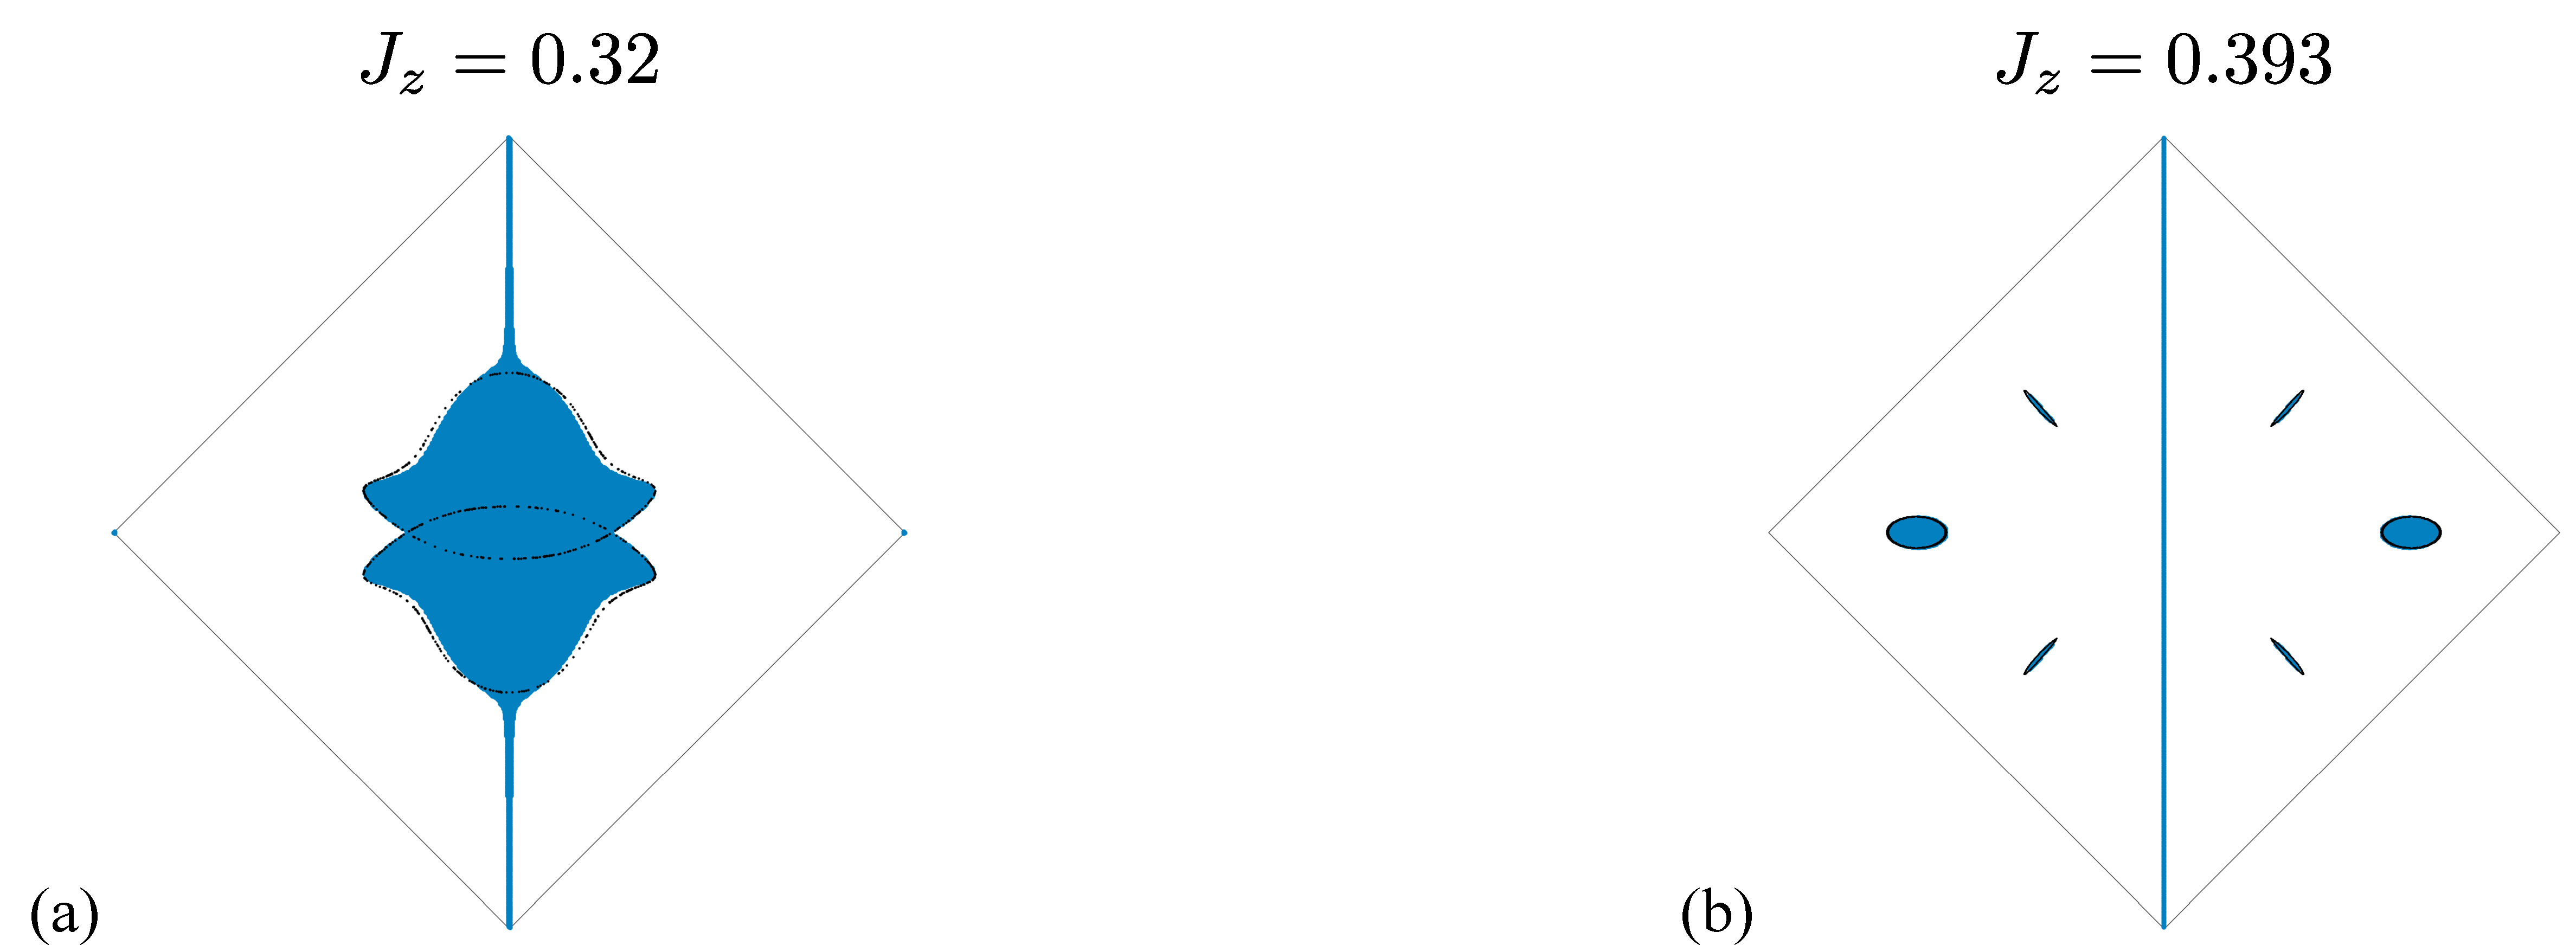
\includegraphics[width=0.8\linewidth]{./chapter06/9_3a_AFIIPanel3.pdf}
	\caption{
		(a) Surface states for $J_z = 0.32$ depicted in blue along with projection of bulk nodal lines depicted in black for the 001-surface Brillouin zone of lattice (9,3)a.
		(b) Surface states for $J_z = 0.393$ depicted in blue along with projection of bulk nodal lines depicted in black for the 001-surface Brillouin zone of lattice (9,3)a.
	}
	\label{fig:chapter06_AFIIPanel3}
\end{figure}
%

For the gapless region corresponding to $J_z \gtrsim 0.392$, a number of nodal lines are stabilized by a one-dimensional \ZZ~winding number.
For $J_z \approx 0.392$, a total of six nodal points appear along high-symmetry lines related to one another by inversion and mirror symmetries or, equivalently, by $C_3$ and inversion symmetries.
The high-symmetry lines themselves correspond to momenta invariant under the combination of mirror and inversion symmetries -- one such line for each of the three mirror planes (see Figure~\ref{fig:chapter06_AFIIPanel2}).
As $J_z$ is increased, the point nodes immediately expand to nodal lines which move through the Brillouin zone and are heavily deformed.
Figure~\ref{fig:chapter06_AFIIPanel2} shows the evolution of the nodal lines for several values of $J_z$.
Due to the severe deformation of the nodal lines which occurs, the figure shows a "top" view from which the deformation is significantly less evident in order to give an overview of their evolution.

From the figure it can already be seen that as $J_z$ is increased slightly, the nodal lines touch before splitting once more to a different total number of nodal lines.
For $J_z \gtrsim 0.42$, there is a transition from the AFII flux phase to the SI flux phase, however, if the analysis is carried out further in the AFII flux configuration, the nodal lines are all seen to combine and shrink to the $\Gamma$-point before gapping out entirely at $J_z \approx 0.45$.
%
\begin{figure}[tb]
	\centering
	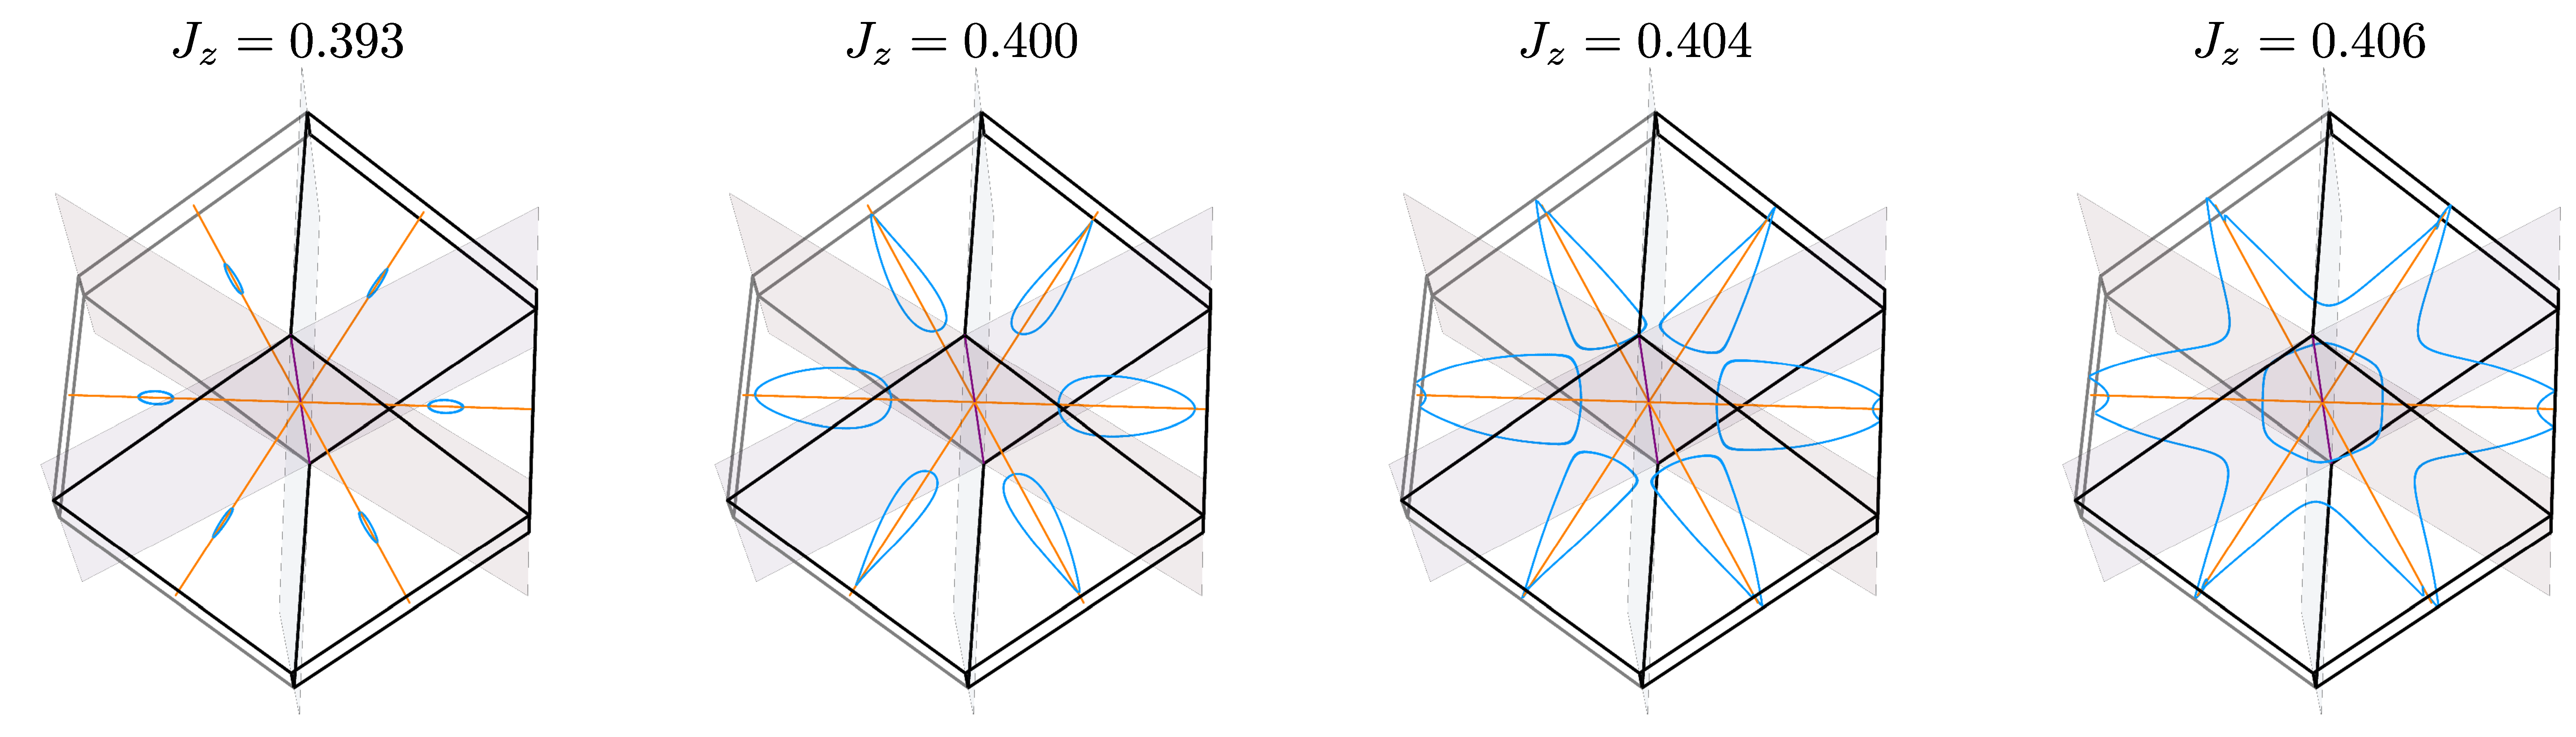
\includegraphics[width=\linewidth]{./chapter06/9_3a_AFIIPanel2.pdf}
	\caption{
		Evolution of nodal lines for several values of $J_z \geq 0.393$ shown in blue.
		The shaded planes denote the three mirror invariant planes, whereas the orange lines denote the $k$-points invariant under a combination of mirror and inversion symmetries.
	}
	\label{fig:chapter06_AFIIPanel2}
\end{figure}
%

Putting the model on a slab geometry (see Figure~\ref{fig:chapter06_AFIIPanel2}~(b)), there are seen to be "drumhead"-type surface states filling the projection of the nodal lines to the surface Brillouin zone as well as the remnant of a Fermi arc from the \ZZ~monopole nodal lines which appear in another part of the phase diagram as discussed above.
However, no Fermi arc like states are observed connecting the disjoint projections of the bulk nodal lines.
The lack of such Fermi arc surface states along with the fact that the bulk nodal lines are not created and destroyed in pairs, rather they appear individually at arbitrary points in the Brillouin zone, indicates that they carry a one-dimensional winding number rather than the two-dimensional monopole charge.


%
%
%%%%%%%%%%%%%%%%%%%%%%%%%%%%%%%%%%%%%%%%%%%%%%%%%%%%%%%%%%%%%%%%%%%%%%%%%%%%%%%%%%%%%%%%
\section{Summary and outlook}
\label{section:chapter06_Conclusion}
%%%%%%%%%%%%%%%%%%%%%%%%%%%%%%%%%%%%%%%%%%%%%%%%%%%%%%%%%%%%%%%%%%%%%%%%%%%%%%%%%%%%%%%%
%
%
This chapter served as a reexamination of the Kitaev model defined on the hypernonagon lattice (9,3)a originally discussed in the work of Reference~\cite{OBrienPRB2016}.
Due to the lattice being non-bipartite, the ground state flux configuration is known to break time-reversal symmetry spontaneously, resulting in a chiral spin liquid ground state.
As mentioned already in Chapter~\ref{chapter:ClassificationOfKSL}, however, the previous analysis of the Kitaev model on this lattice mapped out the fermionic phase diagram using a simple flux configuration which was known not to correspond to the ground state.

In the work reported on in the present chapter, the chiral spin liquids in the entire parameter regime were studied using a combination of finite temperature quantum Monte Carlo simulations, variational calculations and analytic techniques.
The numerics indicate that the phase diagram hosts a variety of chiral spin liquid ground states whose flux sectors depend on the values of the exchange couplings.
A total of five distinct ground state flux configurations were found for different portions of the phase diagram.
While two of these chiral spin liquid ground states are found to be fully gapped, the remaining three ground state flux configurations are seen to correspond to both fully gapped \textit{and} gapless regions in parameter space.

The gapless fermionic excitations in the flux sectors denoted SI and AF are the same Weyl nodes predicted by the classification scheme detailed in Chapter~\ref{chapter:ClassificationOfKSL} which makes use of the projective symmetries of the gauge \textit{Ansatz}.
The analysis of the so-called AFII flux phase, however, sheds light on the possibility of symmetry protected nodal manifolds which were overlooked by the aforementioned classification scheme.
According to this scheme, chiral Kitaev spin liquids cannot host stable nodal lines.
This determination was made based on the inability to define a certain one-dimensional winding number for systems lacking projective time-reversal symmetry~\cite{ZhaoPRL2013,MatsuuraNJP2013}.
However, it has been shown that nodal lines in a three-dimensional system may also be protected by one- or two-dimensional \ZZ~winding numbers in the presence of combined inversion and time-reversal symmetries~\cite{KimPRL2015,FangPRB2015}.
Nodal lines with a \ZZ~monopole charge are seen to exist for a range of exchange couplings in the AFII flux phase.
In yet another parameter regime, this flux phase hosts nodal lines which instead are stabilized by the one-dimensional variant of the \ZZ~winding number.

While much of the results in this chapter are in line with the predictions of the classification scheme detailed in Chapter~\ref{chapter:ClassificationOfKSL}, some results indicate an even richer Kitaev spin liquid physics than previously understood.
The existence of stable monopole nodal lines is possible in principle for any Kitaev spin liquid possessing both inversion and time-reversal symmetries so long as the corresponding projective symmetries are implemented without a finite nesting vector  -- note that this combination of symmetries prevents the formation of stable Weyl nodes.
As seen in this chapter, such nodal lines are also stable for a chiral spin liquid with a broken inversion symmetry, where the combination of time-reversal and inversion operations \textit{does} yield a symmetry.	% Chiral Spin Liquids on the Hypernonagon Lattice (9,3)a
%%%%%%%%%%%%%%%%%%%%%%%%%%%%%%%%%%%%%%%%%%%%%%%%%%%%%%%%%%%%%%%%%%%%%%%%%%%%%%%%%%%%%%%%
\chapter[Correlations in Kitaev Spin Liquids]{Correlations in\linebreak Kitaev Spin Liquids}
\label{chapter:SpinCorrelationsOfKSL}
%%%%%%%%%%%%%%%%%%%%%%%%%%%%%%%%%%%%%%%%%%%%%%%%%%%%%%%%%%%%%%%%%%%%%%%%%%%%%%%%%%%%%%%%
%
%
The last two chapters demonstrated that Kitaev's honeycomb model hosts a broad diversity of gapless quantum spin liquid states when extended to various two- and three-dimensional tricoordinated lattices.
This chapter will explore the consequences which the corresponding gapless modes have on certain equal-time correlation functions of spins.
The focus will be on the spin-spin correlation functions briefly mentioned in Chapter~\ref{chapter:KitaevHoneycombModel} as well as a certain four-spin correlation function, referred to here as the bond-bond correlation function.

While the spin-spin correlations vanish beyond nearest-neighbors, at finite temperature the buildup of these correlations signals a thermodynamic crossover associated to the itinerant Majorana fermions.
The bond-bond correlations, however, intimately reflect the gapless nature of the spin liquids.
Whereas bond-bond correlations are short-ranged in the gapped spin liquid phases, in the \textit{gapless} spin liquid phases the correlation function decays algebraically in a way that depends both on the dimension of the lattice \textit{and} on the character of the gapless modes.
Recently, these bond-bond correlations between pairs of bonds in distinct bipartitions of a honeycomb lattice have been shown to be related to the entanglement entropy~\cite{YangARXIV2019}.
In particular, the quantity obtained by integrating the bond-bond correlation function $\avg{Q_A Q_B} - \avg{Q_A} \avg{Q_B}$ over all bonds $Q$ in the respective bipartitions $A$ and $B$ exhibits the same scaling law as the fermionic contribution to the entanglement entropy for the same bipartition.

It has long been known that the Kitaev honeycomb model defined for \textit{classical} Heisenberg spins hosts a classical spin liquid ground state which can be mapped to a hardcore dimer model.
The classical Kitaev spin liquid also boasts extremely short-ranged spin-spin correlations as well as algebraically decaying bond-bond correlations.
The origin of these algebraic correlations, however, is very different as classical Kitaev spin liquids obviously do not host gapless fermions.
Instead, these correlations are seen to decay in a manner which depends only on the dimension of the underlying lattice.
In Section~\ref{section:chapter07_ClassicalCorrelations}, a very brief introduction to the classical Kitaev model is given along with a discussion of the origins of short-ranged spin-spin correlations and algebraic bond-bond correlations in order to contrast the results of the quantum model.

The rest of this chapter reports on an ongoing study of correlation functions of spins in the \textit{quantum} Kitaev spin liquids.
Section~\ref{section:chapter07_SpinSpinCorrelations} explores the short-ranged spin-spin correlations at both zero temperature and finite temperature, comparing both analytic and numeric results.
Section~\ref{section:chapter07_BondBondCorrelationsZeroTemperature} gives a rather lengthy analysis of the bond-bond correlation functions at zero temperature.
Numerical calculations of bond-bond correlations are presented for a number of two- and three-dimensional lattices for spin liquids hosting Dirac nodes, Fermi lines in two- and three-dimensions, fully two-dimensional Fermi surfaces and Weyl nodes.
A long wavelength analysis is carried out in detail for the two-dimensional lattices to extract the algebraic decay and accompanying Friedel oscillations of the bond-bond correlation function, providing quantitative agreement with the numerics.
Some general remarks and speculations are made for the three-dimensional lattices.
In Section~\ref{section:chapter07_BondBondCorrelationsFiniteTemperature}, expressions for the bond-bond correlation function at finite temperature are derived and briefly discussed.
Section~\ref{section:chapter07_Summary} provides a summary of results and an outlook on some of the unanswered questions in this ongoing work.


%
%
%%%%%%%%%%%%%%%%%%%%%%%%%%%%%%%%%%%%%%%%%%%%%%%%%%%%%%%%%%%%%%%%%%%%%%%%%%%%%%%%%%%%%%%%
\section{A brief introduction to classical Kitaev spin liquids}
\label{section:chapter07_ClassicalCorrelations}
%%%%%%%%%%%%%%%%%%%%%%%%%%%%%%%%%%%%%%%%%%%%%%%%%%%%%%%%%%%%%%%%%%%%%%%%%%%%%%%%%%%%%%%%
%
%
The classical Kitaev honeycomb model, given by the Hamiltonian
%
\begin{equation}
	H = -J_x \sum_{x {\rm -links}} S_j^x S_k^x - J_y \sum_{y {\rm -links}} S_j^y S_k^y - J_z \sum_{z {\rm -links}} S_j^z S_k^z,
\end{equation}
%
where $\bS_j \in O(3)$ correspond to classical Heisenberg spins, was first studied in the context of a \textit{quantum} spin-$S$ Kitaev model~\cite{BaskaranPRB2008}.
It was shown that the classical ground states at the isotropic point correspond to an extensively degenerate manifold wherein each spin perfectly satisfies the local Ising constraint with exactly one of its nearest-neighbors~\cite{BaskaranPRB2008,ChandraPRE2010} (see Figure~\ref{fig:chapter07_DimerPanel}~(a)).
These so-called \textit{dimer} coverings are inherently disordered and spin-spin correlations are non-zero only for nearest-neighbor pairs of dimerized spins~\cite{Ghannad2019}, \ie,
%
\begin{equation}
	\avg{S_j^{\alpha} S_k^{\beta}} = \delta_{\alpha\beta} \delta_{\avg{j,k}_\alpha}.
\end{equation}
%

%
\begin{figure}[tb]
	\centering
	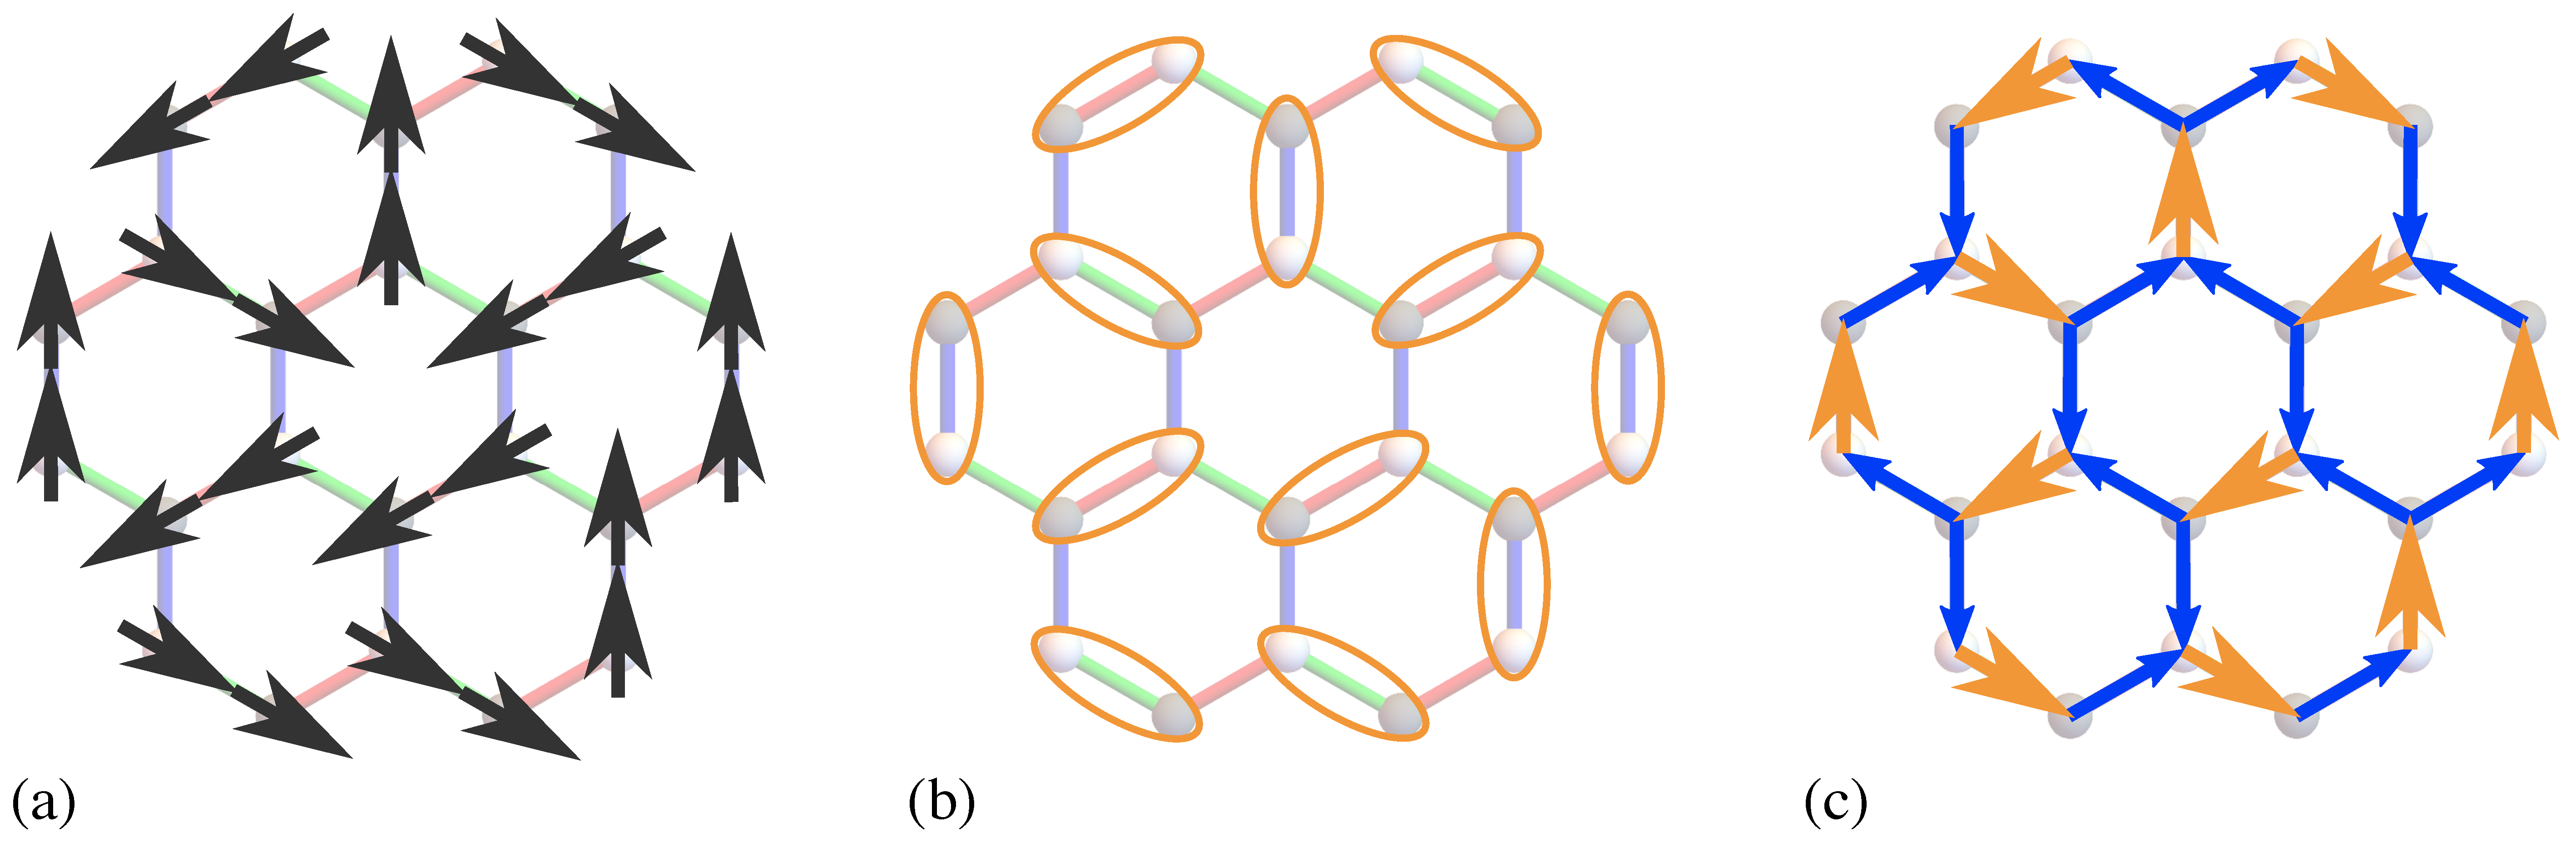
\includegraphics[width=\linewidth]{./chapter07/DimerPanel.pdf}
	\caption{
		One possible ground state of the classical Kitaev honeycomb model represented as (a) a configuration of classical Heisenberg spins, (b) a hardcore dimer covering and (c) a divergence-free polarization field (Figure recreated from Reference~\cite{SelaPRB2014}).
	}
	\label{fig:chapter07_DimerPanel}
\end{figure}
%
Within the ground state manifold, the spin model may be replaced by a model of hardcore dimers which occupy the bonds of the honeycomb lattice (see Figure~\ref{fig:chapter07_DimerPanel}~(b)).
On each $\gamma$-type link one may define a discrete polarization field $\bP(\bR_j, \gamma) = P(\bR_j, \gamma) \hat{\bm{u}}_{\gamma}$ as
%
\begin{equation}
	P(\bR_j, \gamma) = \left\{\begin{matrix*}[l]
		-\frac{1}{3} 				& \text{for non-dimerized links} \\
		\\
		\phantom{-}\frac{2}{3}		& \text{for dimerized links}
	\end{matrix*}\right.
\end{equation}
%
with $\hat{\bm{u}}_{\gamma}$ being the vector connecting the two sites of the link and pointing from sublattice A to sublattice B (see Figure~\ref{fig:chapter07_DimerPanel}~(c)).
This polarization field automatically satisfies a discrete divergence-free condition corresponding to the fact that no dimers may overlap.
The discrete polarization field $\bP(\bR_j, \gamma)$ can be coarse-grained to yield a \textit{continuous} divergence-free polarization field $\bP(\br)$.
It can be argued that the number of dimer covering ground states corresponding to a specific value of the polarization is governed by a Gaussian distribution centered around $\bP = \bz$~\cite{HenleyARCMP2010}.
Defining a free-energy functional for the continuous polarization in terms of the corresponding entropy $S(\{\bP(\br)\})$ as $F(\{\bP(\br)\}) = -T S$, one has that the polarization field satisfies
%
\begin{equation}
	\begin{matrix*}[c]
		F(\{\bP(\br)\})/T = {\rm const} + \frac{1}{2} K \int d^Dr~ \abs{\bP(\br)}^2 \\
		\\
		\bm{\nabla} \cdot \bP(\br) = 0,
	\end{matrix*}
\end{equation}
%
where $D$ is the spatial dimension ($D=2$ for the honeycomb lattice) and $K$ is a constant related to the variance of the Gaussian distribution function for $\bP(\br)$.
As this looks just like the field energy of a magnetic field and its divergence constraint in the absence of monopoles, this state was dubbed a Coulomb phase~\cite{HenleyARCMP2010}.

Dimer-dimer correlations or, equivalently, bond-bond correlations of spins of the form
%
\begin{equation}
	C(\br) = \avg{(S_i^{\gamma}(\bz) S_j^{\gamma}(\bz))(S_k^{\gamma}(\br) S_l^{\gamma}(\br))} - \avg{S_i^{\gamma}(\bz) S_j^{\gamma}(\bz)}\avg{S_k^{\gamma}(\br) S_l^{\gamma}(\br)},
\end{equation}
%
where $i,j$ and $k,l$ are pairs of nearest-neighbor spins connected by a $\gamma$-link, correspond to polarization-polarization correlations which have the spatial dependence of a dipole-dipole interaction at long distances~\cite{HenleyARCMP2010,ChandraPRE2010,SelaPRB2014}, \ie,
%
\begin{equation}
	\avg{P_{\mu}(\bz) P_{\nu}(\br)} \sim \frac{c_D}{K} \frac{(\delta_{\mu\nu} - D \hat{r}_{\mu} \hat{r}_{\nu})}{r^D},
\end{equation}
%
where $c_D$ is a constant which depends on the spatial dimension $D$ and $\hat{\br} = \br/\abs{\br}$.
Thus, despite the disordered nature of the classical spin liquid ground state, the bond-bond correlation function is seen to decay algebraically as $C(\br) \sim 1/r^D$ in a manner which depends only on the dimension of the underlying lattice.


%
%
%%%%%%%%%%%%%%%%%%%%%%%%%%%%%%%%%%%%%%%%%%%%%%%%%%%%%%%%%%%%%%%%%%%%%%%%%%%%%%%%%%%%%%%%
\section{Spin-spin correlations in quantum Kitaev spin liquids}
\label{section:chapter07_SpinSpinCorrelations}
%%%%%%%%%%%%%%%%%%%%%%%%%%%%%%%%%%%%%%%%%%%%%%%%%%%%%%%%%%%%%%%%%%%%%%%%%%%%%%%%%%%%%%%%
%
%
%
%
%%%%%%%%%%%%%%%%%%%%%%%%%%%%%%%%%%%%%%%%%%%%%%%%%%%%%%%%%%%%%%%%%%%%%%%%%%%%%%%%%%%%%%%%
\subsection{Spin-spin correlations at zero temperature}
\label{section:chapter07_SpinSpinCorrelationsZeroTemperature}
%%%%%%%%%%%%%%%%%%%%%%%%%%%%%%%%%%%%%%%%%%%%%%%%%%%%%%%%%%%%%%%%%%%%%%%%%%%%%%%%%%%%%%%%
%
%
As discussed in Section~\ref{section:chapter02_Definition}, all equal-time spin-spin correlation functions of the form
%
\begin{equation}
	S^{\alpha \beta}_{AB}(\bR) = \frac{1}{V} \sum_{\bR'} \avg{\sigma^\alpha_A(\bR') \sigma^\beta_B(\bR'+\bR)}
\end{equation}
%
vanish identically beyond nearest-neighbor spins and for $\alpha \neq \beta \neq \gamma$ as a consequence of flux conservation~\cite{BaskaranPRL2007}, where $\gamma$ denotes the type of bond connecting the two spins, the summation is over all unit cells, $V$ is the system size and $A, B$ denote sites within the unit cell.
The example of a non-vanishing spin-spin correlation function investigated here involves two spins within the same unit cell connected by a z-bond.
Making use of the Majorana representation of Chapter~\ref{chapter:KitaevHoneycombModel}, \ie, $\sigma^{\gamma} = i c^{\gamma} c$, the spin-spin correlation function may be written in terms of two-point functions of Majorana fermions as
%
\begin{align}
	S^{z z}	&= \frac{1}{V} \sum_{\bR'} \avg{\sigma^z_A(\bR') \sigma^z_B(\bR')} \nonumber\\
			&= -\frac{i}{V} \sum_{\bR'} u_{AB}(\bR') \avg{c_A(\bR') c_B(\bR')},
\end{align}
%
where $u_{AB}(\bR')$ is the eigenvalue of the link operator between sites $A$ and $B$ in unit cell $\bR'$.

Having reduced the spin-spin correlation function to a two-point function of Majorana fermions, one may proceed by diagonalizing the fermionic Hamiltonian in a fixed gauge and evaluating the correlation functions with respect to the corresponding fermion vacuum.
Defining complex fermionic operators
%
\begin{equation}
	\begin{matrix*}[l]
		f\dag_{\alpha}	= \frac{1}{\sqrt{2}} \sum_j \psi_{\alpha}^j c_j &
		{\rm and} &
		f_{\alpha}		= \frac{1}{\sqrt{2}} \sum_j \cc{\psi}_{\alpha}^j c_j
	\end{matrix*}
\end{equation}
%
one may express the Majorana operator at site $j$ as
%
\begin{equation}
	c_j = \sqrt{2} \sum_{\alpha} (\cc{\psi}_{\alpha}^j f\dag_{\alpha} + \psi_{\alpha}^j f_{\alpha}),
\end{equation}
%
where $\psi_{\alpha}^j$ is the $j^{\rm th}$ component of the normalized complex eigenvector of the Kitaev Hamiltonian in a fixed gauge corresponding to the eigenenergy $\epsilon_{\alpha}$ and the bar is used to denote complex conjugation.
Due to the inherent particle-hole symmetry of the Majorana representation, only half of the eigenstates of the Hamiltonian correspond to independent complex fermionic states.
In the following, the convention will be used that creation operators all correspond to non-negative eigenenergies.
While this convention suffices for the following and is most convenient in the context of numerical calculations, other conventions will be seen in subsequent sections to be more suitable for analytic calculations.

Using this convention, the Majorana two-point functions $\avg{c_j c_k}$ may be evaluated as
%
\begin{align}
	\avg{c_j c_k}	&= 2 \sum_{\alpha, \beta} \avg{ \left( \overline{\psi}^j_\alpha ~f\dag_\alpha + \psi^j_\alpha ~f_\alpha \right) \left( \overline{\psi}^k_\beta ~f\dag_\beta + \psi^k_\beta ~f_\beta \right) } \nonumber\\
					&= 2 \sum_{\alpha, \beta} \psi^j_\alpha ~\overline{\psi}^k_\beta \avg{ f_\alpha f\dag_\beta } \nonumber\\
					&= 2 \sum_\alpha \psi^j_\alpha ~\overline{\psi}^k_\alpha.
	\label{eq:chapter07_TwoPointFermionZeroT}
\end{align}
%
Although the above expectation values are taken with respect to the fermion vacuum, expectation values may easily be taken with respect to any arbitrary many-fermion state (in a fixed gauge) simply by swapping the particle and hole wave functions for the occupied single-particle states.
From the anti-commutativity of the Majorana operators, it is straightforward to see that the contribution to the two-point function due to the occupied single-particle state will differ from its ground state counterpart only by a minus sign, \ie,
%
\begin{equation}
	\avg{c_j c_k}_{\{n_\alpha\}} = 2 \sum_{\alpha=1}^N (-1)^{n_\alpha} \psi^j_\alpha ~\overline{\psi}^k_\alpha,
\end{equation}
%
where $\avg{\ldots}_{\{n_\alpha\}}$ denotes an expectation value with respect to the many-fermion state with occupation numbers $\{n_\alpha\}$.
As a result, a Majorana two-point function evaluated with respect to two different many-fermion states which have opposite single-particle occupation numbers will be identical in magnitude, but opposite in sign.

Putting everything together, the spin-spin correlation function may be evaluated in terms of the complex fermionic wave functions as
%
\begin{equation}
	S^{z z}	= -\frac{2i}{V} \sum_{\bR', \alpha} u_{AB}(\bR')~\psi_{\alpha}^A(\bR') \cc{\psi}_{\alpha}^B(\bR'),
	\label{eq:chapter07_TwoSpinZeroT}
\end{equation}
%
where $\psi_{\alpha}^{A/B}(\bR')$ corresponds to the component of the wave function $\psi_{\alpha}$ at site $A/B$ in unit cell $\bR'$.


%
%
%%%%%%%%%%%%%%%%%%%%%%%%%%%%%%%%%%%%%%%%%%%%%%%%%%%%%%%%%%%%%%%%%%%%%%%%%%%%%%%%%%%%%%%%
\subsection{Spin-spin correlations at finite temperature}
\label{section:chapter07_SpinSpinCorrelationsFiniteTemperature}
%%%%%%%%%%%%%%%%%%%%%%%%%%%%%%%%%%%%%%%%%%%%%%%%%%%%%%%%%%%%%%%%%%%%%%%%%%%%%%%%%%%%%%%%
%
%
Given Eq.~\eqref{eq:chapter07_TwoSpinZeroT} in the last section, one may simply diagonalize the Kitaev Hamiltonian in a gauge configuration compatible with the ground state flux sector and use the resulting eigenvectors to calculate the zero temperature spin-spin correlation functions.
Other than it being extremely short-ranged, this quantity is not very interesting on its own.
What may be interesting, however, is the way these correlations behave in the presence of thermal fluctuations.

A number of quantum Monte Carlo studies have been performed on Kitaev spin liquids in both two- and three-dimensions~\cite{NasuPRB2014,NasuPRL2014,NasuJoP2015,NasuPRB2015,NasuPRL2015,NasuJoP2016,MischenkoPRB2017,EschmannPRL2019} revealing \textit{nearly} universal behavior, namely, an ordering of the gauge field at low temperature ($T \sim 10^{-2}$ times the exchange couplings) in a crossover or transition in two- and three-dimensions, respectively, and a higher-temperature crossover (on the order of the exchange couplings) typically attributed to the itinerant Majorana fermions (see Figure~\ref{fig:chapter07_6_3SpinSpinCorrelations}).
Each of the two features in the specific heat curve correspond to a release of one half the total entropy of the system.
Furthermore, the high-temperature crossover is seen to coincide with the onset of nearest-neighbor spin-spin correlations.

In order to investigate the nature of this crossover further, analytic expressions for the spin-spin correlation function at \textit{finite temperature} are derived here.
In a fixed gauge configuration, the thermal expectation value of a Majorana two-point function at temperature $T=1/\beta$ is given by
%
\begin{equation}
	\avg{\avg{c_j c_k}}_{T} = \frac{1}{Z} \sum_{\{n_\alpha\}_{\alpha=1}^N} \avg{c_j c_k}_{\{n_\alpha\}} \exp{\left[ -\beta\sum_{\lambda=1}^N \epsilon_\lambda (n_\lambda-1/2) \right]},
\end{equation}
%
where $N$ is the number of single-particle states, $\epsilon_{\lambda}$ are the single-particle energies, $n_\alpha \in \{ 0, 1\}$ is the occupation number of the single-particle state $\psi_\alpha$, the bracketed expression $\avg{\ldots}_{\{n_\alpha\}}$ denotes an expectation value with respect to the many-fermion state with occupation numbers $\{n_\alpha\}$, and the fermionic partition function $Z$ for the fixed gauge is given by
%
\begin{equation}
	Z = \sum_{\{n_\alpha\}_{\alpha=1}^N} \exp{\left[ -\beta \sum_{\lambda=1}^N \epsilon_\lambda (n_\lambda - 1/2) \right]}.
\end{equation}
%

%
\begin{figure}[tb]
	\centering
	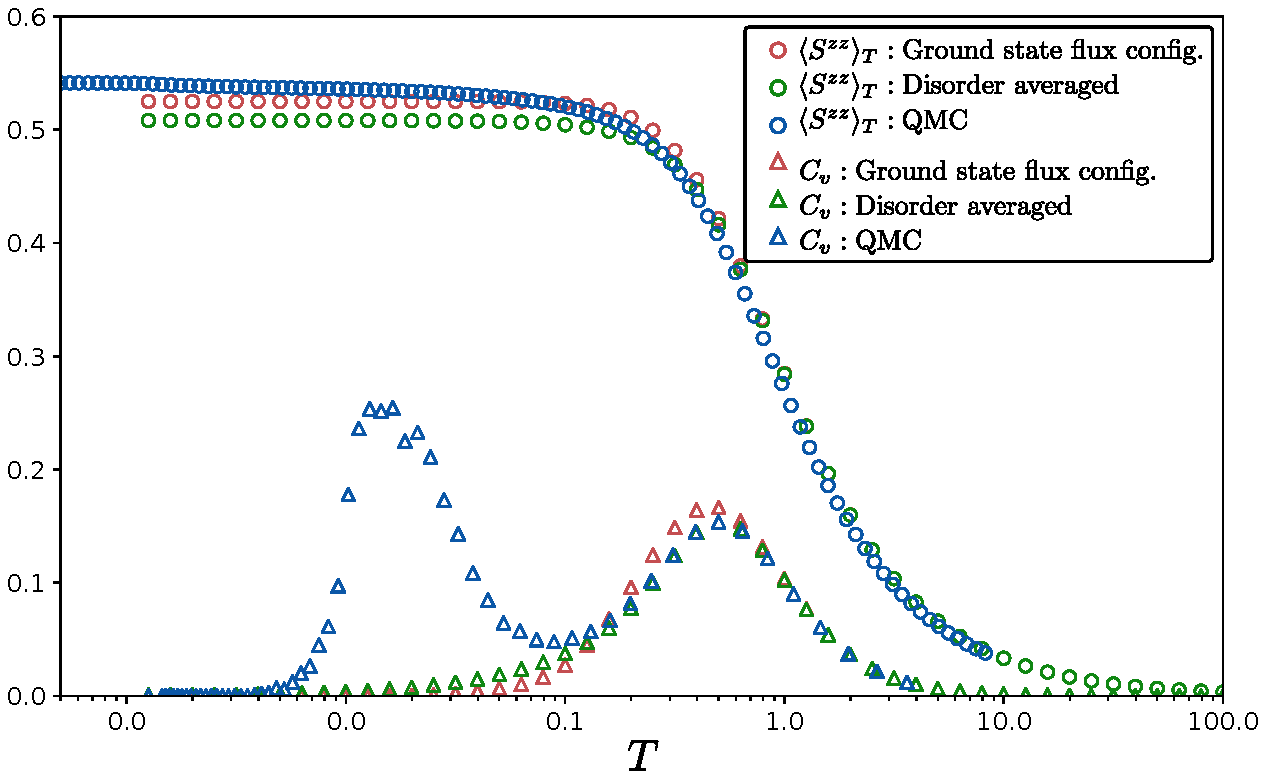
\includegraphics[width=0.8\linewidth]{./chapter07/HoneycombFiniteTempSpinSpinCorrelations.pdf}
	\caption{
		Nearest neighbor spin-spin correlations $S^{zz}$ and specific heat $C_v$ as a function of temperature for the Kitaev model on the honeycomb lattice.
		Comparison of a fixed ground state flux configuration (blue), averaging over random flux configurations (orange), and quantum Monte Carlo simulation (green).
	}
	\label{fig:chapter07_6_3SpinSpinCorrelations}
\end{figure}
%
To avoid explicitly performing the trace over all many-particle states, the above expressions are simplified as follows
(for notational simplicity, let $\Theta_\lambda = \beta \epsilon_\lambda/2$ and $\chi^{jk}_\mu = \psi^j_\mu \overline{\psi}^k_\mu$ in the following).
The fermionic partition function may be evaluated as
%
\begin{align}
	Z 	&= \sum_{\{n_\alpha\}_{\alpha=1}^N} \prod_{\lambda=1}^N \exp{\Big[(-1)^{n_\lambda} \Theta_\lambda\Big]} \nonumber\\
		&= \sum_{\{n_\alpha\}_{\alpha=2}^N} \sum_{n_1=0,1} \exp{[(-1)^{n_1} \Theta_1]} \prod_{\lambda=2}^N \exp{\Big[(-1)^{n_\lambda} \Theta_\lambda\Big]} \nonumber\\
%		&= 2\cosh{[\Theta_1]} \sum_{\{n_\alpha\}_{\alpha=2}^N} \prod_{\lambda=2}^N \exp{\Big[(-1)^{n_\lambda} \Theta_\lambda\Big]} \nonumber\\
		&= \prod_{\lambda=1}^N 2\cosh{[\Theta_\lambda]}.
\end{align}
%
The thermal Majorana two-point function can be simplified in an analogous manipulation as
%
\begin{align}
	\avg{\avg{c_j c_k}}_{T} &= \frac{1}{Z} \sum_{\{n_\alpha\}_{\alpha=1}^N} \avg{c_j c_k}_{\{n_\alpha\}} \exp{\Big[ -\beta \sum_{\lambda=1}^N \epsilon_\lambda (n_\lambda - 1/2) \Big]} \nonumber\\
							&= \frac{2}{Z} \sum_{\{n_\alpha\}_{\alpha=1}^N} \sum_{\mu=1}^N (-1)^{n_\mu} \chi^{jk}_\mu \prod_{\lambda=1}^N \exp{\Big[ (-1)^{n_\lambda} \Theta_\lambda \Big]} \nonumber\\
							&~~\vdots \nonumber\\
							&= \frac{2}{Z} \sum_{\mu=1}^N \chi^{jk}_\mu \tanh{[\Theta_\mu]} \prod_{\lambda=1}^N 2 \cosh{[\Theta_\lambda]} \nonumber\\
							&= 2 \sum_{\mu=1}^N \chi^{jk}_\mu \tanh{[\Theta_\mu]}.
\end{align}
Finally, the thermal spin-spin correlation function may be written in a fixed gauge as
\begin{align}
	\avg{S^{z z}}_T &= -\frac{i}{V} \sum_{\bR'} u_{AB}(\bR') \avg{\avg{c_A(\bR') c_B(\bR')}}_{T} \nonumber\\
					&= -\frac{2i}{V} \sum_{\bR'} u_{AB}(\bR') \sum_{\mu=1}^N \psi_\mu^A(\bR') \overline{\psi}_\mu^B(\bR') \tanh{[\beta \epsilon_\mu / 2]}.
	\label{eq:chapter07_ThermalSpinSpin}
\end{align}
%

Assuming a ground state gauge \textit{Ansatz}, the ground state expectation value is recovered as $T\rightarrow 0$.
Regardless of the gauge or flux configuration chosen, for $T\rightarrow \infty$ the spin-spin correlations vanish due to $\lim_{x\rightarrow 0} \left[\tanh{x}\right] = 0$.
For a more physical picture, recall from the last section that many-fermion states with complementary single-particle occupation numbers result in an equal but opposite contribution to a Majorana two-point function.
At high temperature where all states are weighted equally, contributions from such pairs of states will cancel each other, resulting in a vanishing of spin-spin correlations.
While the above analysis ignored thermal fluctuations of the gauge field by assuming a static configuration, the qualitative results are independent of this fact.
Moreover, for temperatures far enough above the gauge-field-disordering-crossover/transition, a simple averaging over random flux configurations may substitute the full-blown quantum Monte Carlo simulation.
%
\begin{figure}[tb]
	\centering
	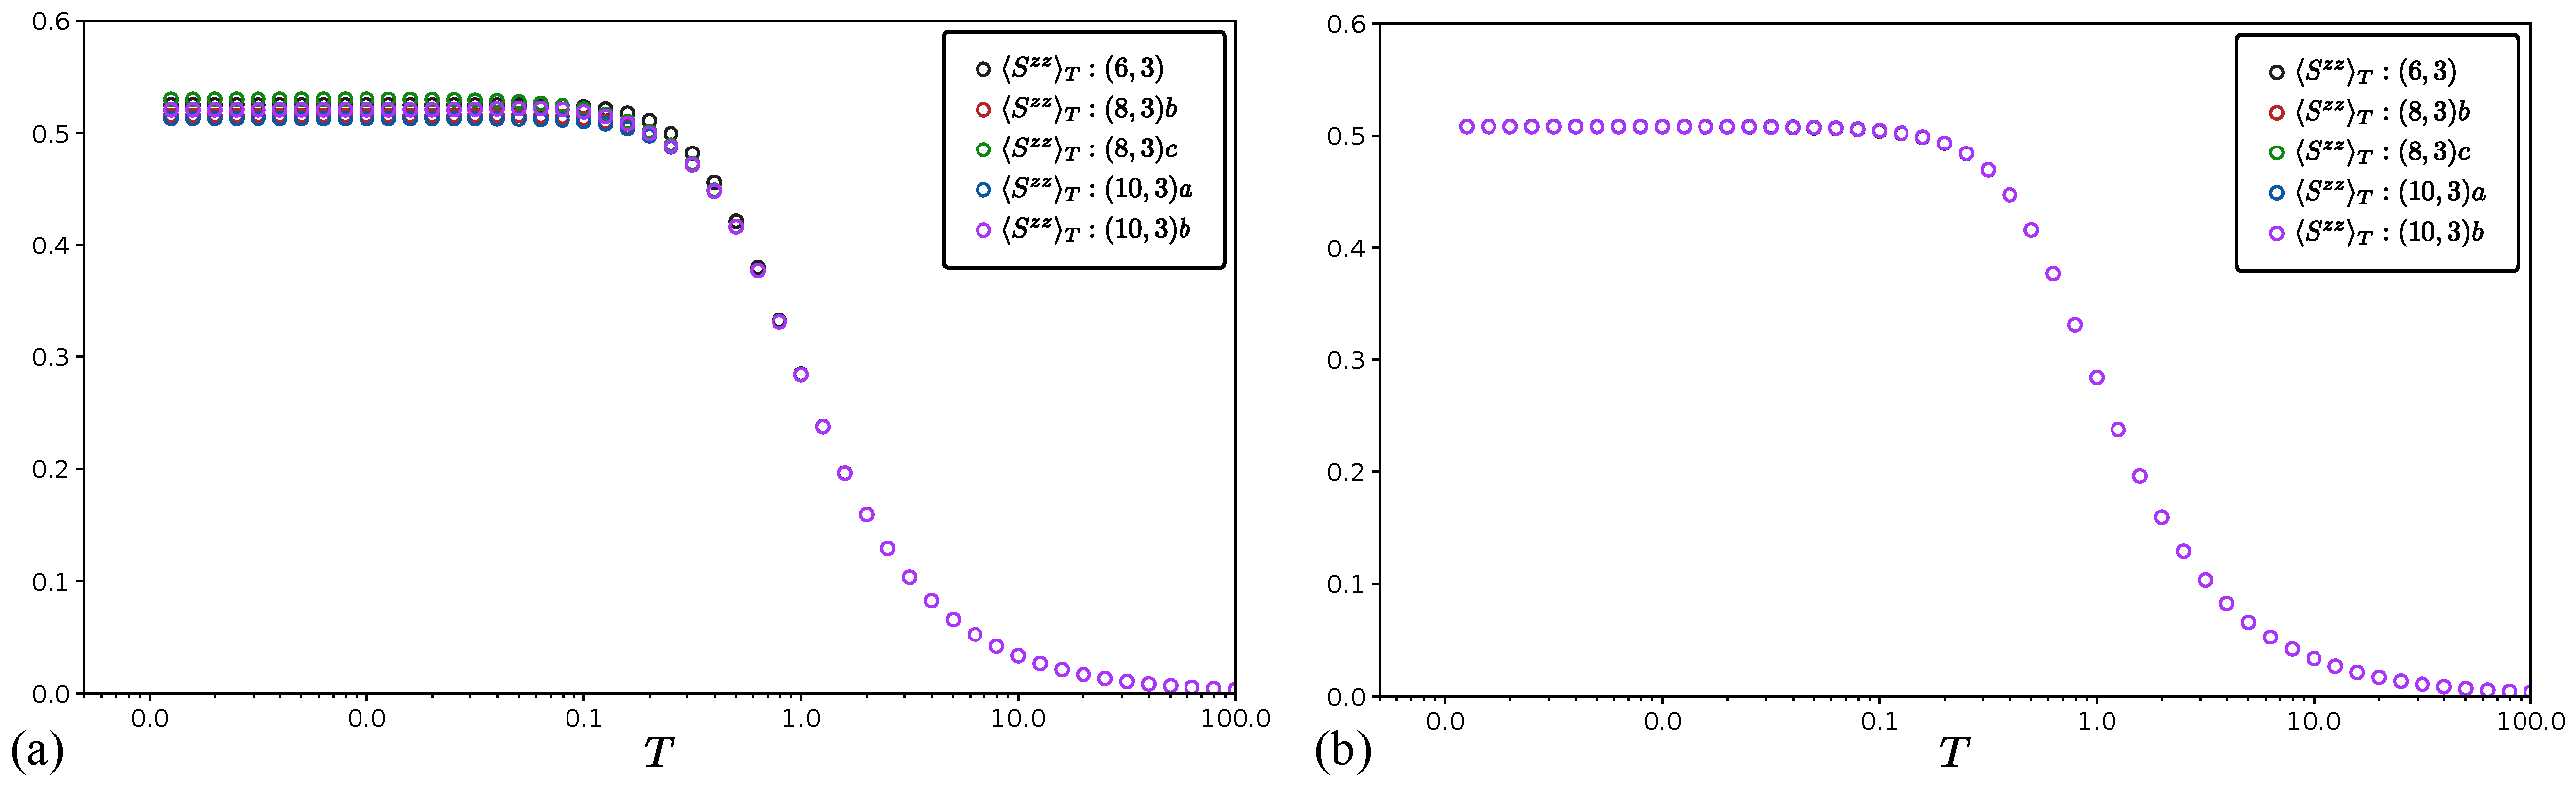
\includegraphics[width=\linewidth]{./chapter07/LatticesFiniteTempSpinSpinCorrelations.pdf}
	\caption{
		Nearest neighbor spin-spin correlations $S^{zz}$ and specific heat $C_v$ as a function of temperature for the Kitaev model on lattices (6,3), (8,3)b, (8,3)c, (10,3)a and (10,3)b.
		(a) Observables calculated in a fixed, ground state flux configuration.
		(b) Observables averaged over random flux configurations.
	}
	\label{fig:chapter07_LatticesSpinSpinCorrelations}
\end{figure}
%

In Figure~\ref{fig:chapter07_6_3SpinSpinCorrelations} are plotted three different data sets for the nearest-neighbor spin-spin correlation function $\avg{S^{zz}}_T$ and the specific heat $C_v$ for the honeycomb lattice as functions of temperature.
For the data set colored in blue, Eq.~\eqref{eq:chapter07_ThermalSpinSpin} was used to calculate the correlation function $\avg{S^{zz}}_T$ using a fixed gauge corresponding to the ground state flux configuration.
The specific heat was calculated directly from the single-particle spectrum.
The orange colored data set was similarly calculated from Eq.~\eqref{eq:chapter07_ThermalSpinSpin}, but this time the data was averaged over a large number of \textit{random} flux configurations.
Finally, the green data is taken from a quantum Monte Carlo simulation.

Although the correlations at very low temperature measured via quantum Monte Carlo are a little too large due to finite size effects, one can see from the figure that the data smoothly interpolates between the ground state flux sector data and the random flux sector data as temperature is increased.
Above the low-temperature crossover, the disorder-averaged data fits extremely well to the Monte Carlo simulation data.
In fact, the difference between the data calculated for the ground state flux sector differs very little from the disorder averaged data.
The disordering of the fluxes does not appear to shift the high-temperature crossover and, in general, only seems to suppress the value of the correlations slightly.
It was pointed out in Reference~\cite{NasuPRB2015} that as the fluxes become disordered, the linear scaling of the density of states near zero energy from the clean system is replaced by a finite density of states at zero energy. 
It may be that this large spectral weight at low energy is responsible for the suppression of correlations due to it being easier to excite many-fermion states at lower temperatures.

For a fixed density of \ZZ~fluxes -- whether that of the ground state flux sector or the maximally disordered flux configurations -- the spin-spin correlations are nearly constant up until the crossover temperature where excited many-fermion states destroy the correlations.
Coupled with the simultaneous release of fermionic entropy, this suggests that below the crossover temperature the only substantial contributions come from the fermionic ground state.

Finally, in Figure~\ref{fig:chapter07_LatticesSpinSpinCorrelations} are plotted the nearest neighbor spin-spin correlations $S^{zz}$ and specific heat $C_v$ as a function of temperature for the honeycomb lattice as well as a number of three-dimensional lattices -- both for a fixed ground state flux configuration and averaged over random flux configurations.
From Figure~\ref{fig:chapter07_LatticesSpinSpinCorrelations}~(a) the ground state value of the spin-spin correlations is seen to vary slightly from lattice to lattice, although the decay of correlations occurs at the same temperature.
However, when averaged over random flux configurations, the data is indistinguishable for the different lattices, as seen in Figure~\ref{fig:chapter07_LatticesSpinSpinCorrelations}~(b).
This is not so surprising as the low-energy density of states governing the low-temperature correlations for the disordered systems is in all cases governed by random matrix theory for the symmetry class BDI, and the center of mass of the single-particle density of states likely to control the position of the crossover is only slightly affected by disorder.
%
\begin{table}[tb]
	\centering
	\resizebox{\textwidth}{!}
	{\begin{tabular}{llrr}
		\hline
		\textbf{Lattice}             & \textbf{Gapless modes}	&	& \textbf{Exponent ($\alpha \approx d + d_c$)}     	\\ \hline
		\textbf{2D}                  & 							&	&							\\
		Square-octagon				 & Fermi line 				&	& 3.06 $\pm$ 0.08~~ 			$\approx~ 2 + 1$ \\
		Honeycomb					 & Dirac nodes        		&	& 3.995 $\pm$ 0.002~~ 		$\approx~ 2 + 2$ \\
		\textbf{3D}                  & 							&	&							\\
		(10,3)a 					 & Fermi surface     		&	& 3.93 $\pm$ 0.46~~ 			$\approx~ 3 + 1$ \\
		(10,3)b						 & Fermi line        		& In-plane:		& 5.15 $\pm$ 0.50~~	 $\approx~ 3 + 2$		\\
		& 							& Out-of-plane:	& 4.06 $\pm$ 0.01~~ 	 $\approx~ 4\;\,\phantom{+ 1}$			\\
		(10,3)c						 & Fermi line        		& In-plane: 	& 4.99 $\pm$ 0.30~~	 $\approx~ 3 + 2$		\\
		& 							& Out-of-plane:	& 3.96 $\pm$ 0.29~~	 $\approx~ 4\;\, \phantom{+ 1}$	 		\\
		(8,3)b 						 & Weyl nodes        		&	& 6.00 $\pm$ 0.06~~	 $\approx~ 3 + 3$ 		\\
	\end{tabular}}
	\caption{
		Overview of algebraic bond-bond correlations in gapless Kitaev spin liquids.
		The leading order long-wavelength behavior is seen to be given by $C(\br) \sim 1/\abs{\br}^{d + d_c}$, where $d$ is the spatial dimension and $d_c$ is the codimension of the nodal manifold.
	}
	\label{table:chapter07_BondBondCorrelations}
\end{table}
%
\newpage


%
%
%%%%%%%%%%%%%%%%%%%%%%%%%%%%%%%%%%%%%%%%%%%%%%%%%%%%%%%%%%%%%%%%%%%%%%%%%%%%%%%%%%%%%%%%
\section[Bond-bond correlations at zero temperature]{Bond-bond correlations at zero temperature}
\label{section:chapter07_BondBondCorrelationsZeroTemperature}
%%%%%%%%%%%%%%%%%%%%%%%%%%%%%%%%%%%%%%%%%%%%%%%%%%%%%%%%%%%%%%%%%%%%%%%%%%%%%%%%%%%%%%%%
%
%
%%%%%%%%%%%%%%%%%%%%%%%%%%%%%%%%%%%%%%%%%%%%%%%%%%%%%%%%%%%%%%%%%%%%%%%%%%%%%%%%%%%%%%%%
\subsection{General considerations and numerics}
\label{section:chapter07_BondBondGeneral}
%%%%%%%%%%%%%%%%%%%%%%%%%%%%%%%%%%%%%%%%%%%%%%%%%%%%%%%%%%%%%%%%%%%%%%%%%%%%%%%%%%%%%%%%
%
%
%%
%\begin{table}[tb]
%	\centering
%	\label{my-label}
%	\begin{tabular}{llrrr}
%		\hline
%		\textbf{Lattice}             & \textbf{Gapless modes}	&	& \textbf{Exponent ($\alpha \approx d + d_c$)}     	\\ \hline
%		\textbf{2D}                  & 							&	&							\\
%		Square-octagon				 & Fermi line 				&	& 3.06 $\pm$ 0.08~~ 			$\approx~ 3$	& $= 2 + 1$ \\
%		Honeycomb					 & Dirac nodes        		&	& 3.995 $\pm$ 0.002~~ 		$\approx~ 4$	& $= 2 + 2$ \\
%		\textbf{3D}                  & 							&	&							\\
%		(10,3)a 					 & Fermi surface     		&	& 3.93 $\pm$ 0.46~~ 			$\approx~ 4$	& $= 3 + 1$ \\
%		(10,3)b						 & Fermi line        		& In-plane:		& 5.15 $\pm$ 0.50~~	 $\approx~ 5$	& $= 3 + 2$		\\
%		& 							& Out-of-plane:	& 4.06 $\pm$ 0.01~~ 	 $\approx~ 4$	&		\\
%		(10,3)c						 & Fermi line        		& In-plane: 	& 4.99 $\pm$ 0.30~~	 $\approx~ 5$	& $= 3 + 2$		\\
%		& 							& Out-of-plane:	& 3.96 $\pm$ 0.29~~	 $\approx~ 4$	& 		\\
%		(8,3)b 						 & Weyl nodes        		&	& 6.00 $\pm$ 0.06~~	 $\approx~ 6$	& $= 3 + 3$ 		\\
%	\end{tabular}
%	\caption{
%		Overview of algebraic bond-bond correlations in gapless Kitaev spin liquids.
%		The leading order long-wavelength behavior is seen to be given by $C(\br) \sim 1/\abs{\br}^{d + d_c}$, where $d$ is the spatial dimension and $d_c$ is the codimension of the nodal manifold.
%	}
%	\label{table:chapter07_BondBondCorrelations}
%\end{table}
%%
In order to compute bond-bond correlations of the form
%
\begin{align}
	C(\bR) 	&= \frac{1}{V} \sum_{\bR'} \Big( \avg{\big(\sigma^z_A(\bR') \sigma^z_B(\bR')\big) \big(\sigma^z_A(\bR'+\bR) \sigma^z_B(\bR'+\bR)\big)}\nonumber\\
			&\qquad- \avg{\sigma^z_A(\bR') \sigma^z_B(\bR')} \avg{\sigma^z_A(\bR'+\bR) \sigma^z_B(\bR'+\bR)} \Big),
\end{align}
%
the spin operators should be expressed in the Majorana representation and the resulting Majorana four-point functions may be evaluated in terms of the Majorana two-point functions of the last section using Wick's theorem as
%
\begin{align}
	C(\bR) 	&= -\frac{4}{V} \sum_{\bR'} u_{AB}(\bR') u_{AB}(\bR' + \bR)~\times \nonumber\\
			&\qquad\sum_{\mu,\nu} \Bigg[\Big(\psi_{\mu}^A(\bR') \overline{\psi}_{\mu}^A(\bR' + \bR)\Big) \Big(\psi_{\nu}^B(\bR' + \bR) \overline{\psi}_{\nu}^B(\bR') \Big) \nonumber\\
			&\qquad\qquad+ \Big(\psi_{\mu}^A(\bR') \overline{\psi}_{\nu}^A(\bR' + \bR)\Big) \Big(\psi_{\nu}^B(\bR') \overline{\psi}_{\mu}^B(\bR' + \bR) \Big)\Bigg],
\end{align}
%
where the Greek indices are summed over single-particle states with non-negative energies as before.
For a translationally invariant system, \eg, at zero temperature, bond-bond correlations may be expressed particularly simply in terms of their Fourier components as
%
\begin{equation}
	C(\bR) = \frac{1}{\sqrt{V}} \sum_{\bk} e^{\-i \bk\cdot\bR} \tilde{C}(\bk)
	\label{eq:chapter07_BondBondInverseFourier}
\end{equation}
%
with
%
\begin{align}
	\tilde{C}(\bk) =	&-\frac{4}{V^{3/2}} \sum_{\bq} \sum_{\alpha,\beta} \Bigg[ \left|\psi_{\alpha}^A(\bk + \bq)\right|^2 \left|\psi_{\beta}^B(\bq)\right|^2 \nonumber\\
						&\qquad\qquad+ \left(\psi_{\alpha}^A(\bk + \bq) \overline{\psi}_{\beta}^A(\bq)\right) \left(\psi_{\beta}^B(\bq) \overline{\psi}_{\alpha}^B(\bk + \bq)\right) \Bigg],
	\label{eq:chapter07_BondBondZeroTFourier}
\end{align}
%
where the momenta are summed over the entire first Brillouin zone and $\alpha,\beta$ are band indices summed over non-negative energies at each momentum.

Eq.~\eqref{eq:chapter07_BondBondZeroTFourier} was used to numerically calculate bond-bond correlations in momentum space for the Kitaev model at the isotropic point ($J_x = J_y = J_z$) on a number of two- and three-dimensional lattices.
The real space data pictured in Figure~\ref{fig:chapter07_6_3BondBondPanel} was then arrived at by inverse Fourier transformation according to Eq.~\eqref{eq:chapter07_BondBondInverseFourier}.
While bond-bond correlations decay exponentially in the gapped spin liquid phases~\cite{YangPRA2008}, from Figure~\ref{fig:chapter07_6_3BondBondPanel} one may see that the gapless spin liquid phases exhibit algebraically decaying bond-bond correlations $C(\br) \sim 1/r^{\alpha}$, where the integer exponent $\alpha$ depends on the character of the gapless spin liquid.

The observation directions $\br$ shown in the plots of Figure~\ref{fig:chapter07_6_3BondBondPanel} were chosen to minimize the Friedel oscillations wherever possible.
The exponents $\alpha$ were found by fitting the log-log scaled data to a linear curve, ignoring the Friedel oscillations.
Table~\ref{table:chapter07_BondBondCorrelations} displays the different lattices along with the type of gapless modes it exhibits and the corresponding decay exponent $\alpha$.
Note that calculations for the square-octagon lattice are performed in the zero flux sector rather than in the ground state $\pi$-flux sector due to the ground state sector being gapless~\cite{YangPRB2007}.
From the data it can be seen that the decay exponent depends on both the dimension of the lattice \textit{and} the dimension of the nodal manifold.
Additionally, it can be seen in the case of Fermi lines in a three-dimensional Kitaev spin liquid that the value of the exponent depends on the observation direction $\br$.
While the power law fits to the data do not explain the presence of Friedel oscillations and yield approximately integer exponents, the next section provides a more detailed asymptotic analysis of the bond-bond correlation functions thereby demonstrating the origins of both.
%
\begin{figure}[p]
	\centering
	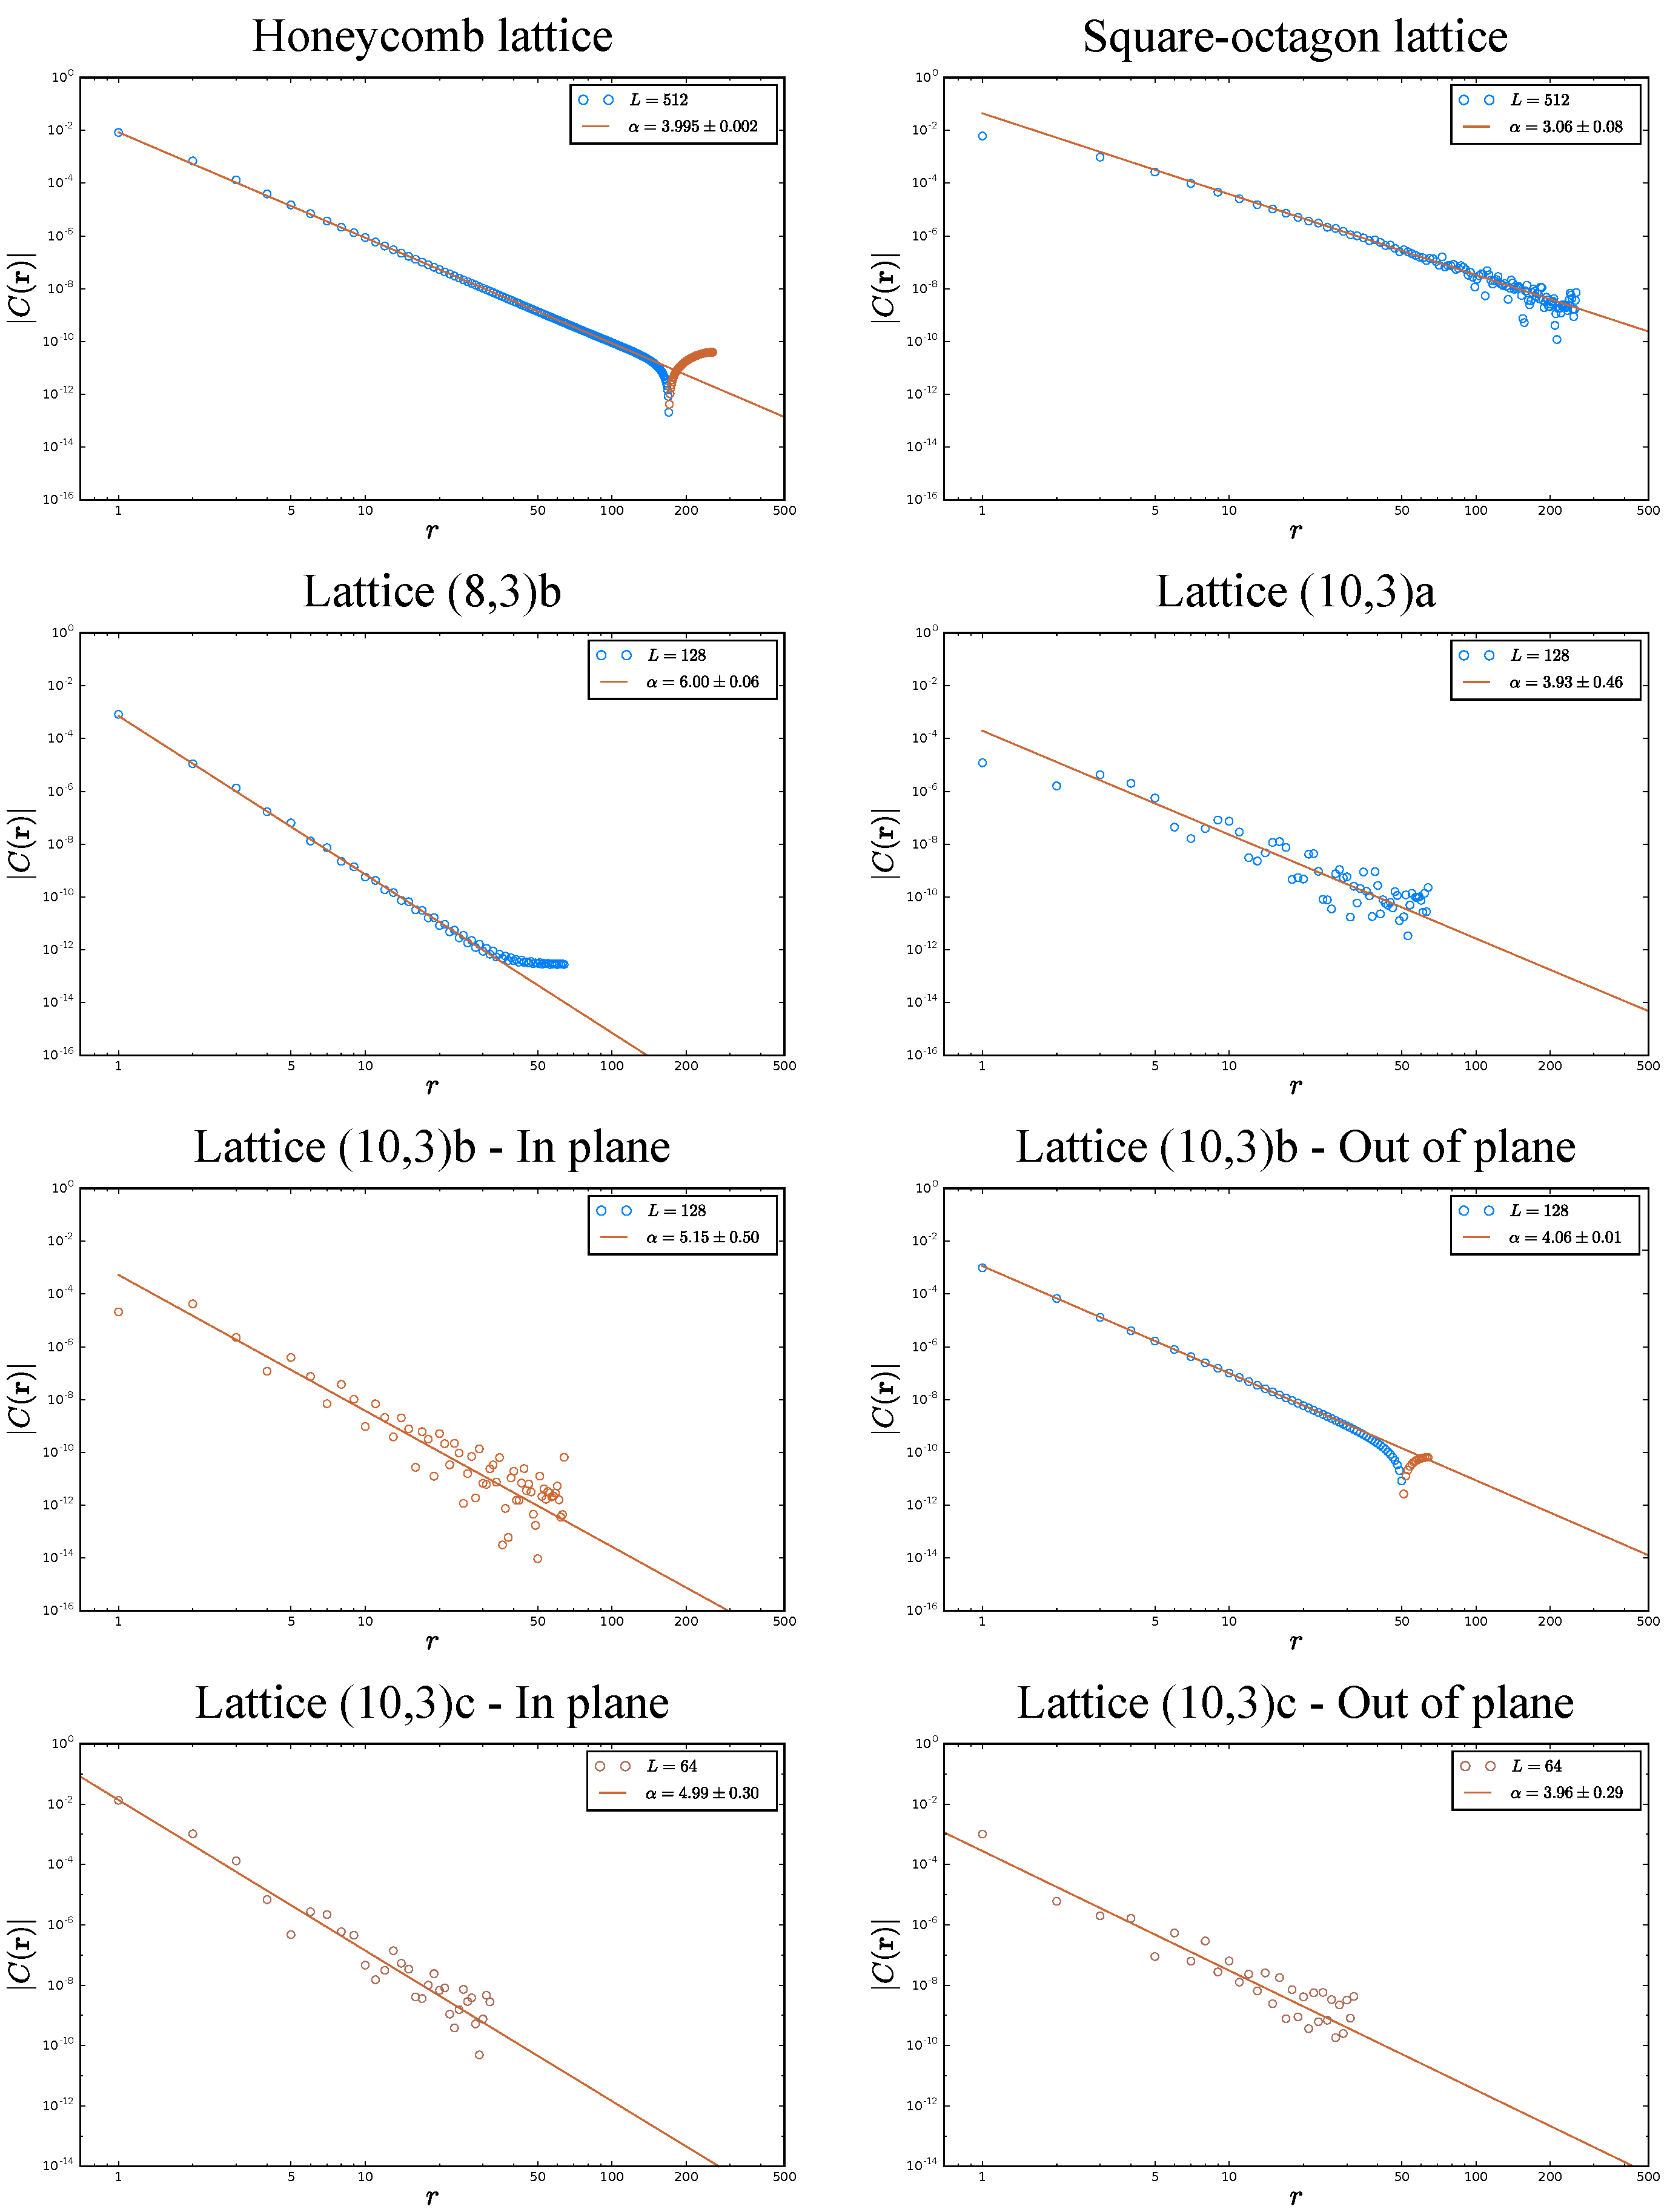
\includegraphics[width=\linewidth]{./chapter07/BondBondPanel.pdf}
	\caption{
		Bond-bond correlations $\abs{C(\br)}$ plotted on a log-log scale for gapless Kitaev spin liquids on a number of two- and three-dimensional lattices with $J_x = J_y = J_z$.
		Circles correspond to numerical data, whereas lines correspond to a linear fit through the data.
		The data is color coded blue and orange corresponding to positive and negative values of $C(\br)$, respectively.
		The two-dimensional honeycomb and square-octagon lattices host Dirac nodes and Fermi lines, respectively.
		The three-dimensional (8,3)b and (10,3)a lattices host Weyl nodes and Fermi surfaces, respectively, while lattices (10,3)b and (10,3)c host Fermi lines.
		Two directions are shown for lattices (10,3)b and (10,3)c corresponding to observation directions $\br$ both parallel (in plane) and perpendicular (out of plane) to the plane in which the Fermi line lies.
	}
	\label{fig:chapter07_6_3BondBondPanel}
\end{figure}
%


%
%
%%%%%%%%%%%%%%%%%%%%%%%%%%%%%%%%%%%%%%%%%%%%%%%%%%%%%%%%%%%%%%%%%%%%%%%%%%%%%%%%%%%%%%%%
\subsection{Asymptotic evaluation of correlation functions}
\label{section:chapter07_BondBondNumerics}
%%%%%%%%%%%%%%%%%%%%%%%%%%%%%%%%%%%%%%%%%%%%%%%%%%%%%%%%%%%%%%%%%%%%%%%%%%%%%%%%%%%%%%%%
%
%
In exploring the asymptotic behavior of the ground state bond-bond correlation functions, a translationally invariant gauge is assumed in order to yield
%
\begin{align}
	C(\br)	&= \avg{\sigma_A^z(\bz) \sigma_B^z(\bz) \sigma_A^z(\br) \sigma_B(\br)} - \avg{\sigma_A^z(\bz) \sigma_B^z(\bz)} \avg{\sigma_A^z(\br) \sigma_B^z(\br)} \nonumber\\
			&= \avg{c_A(\bz) c_A(\br)} \avg{c_B(\bz) c_B(\br)} - \avg{c_A(\bz) c_B(\br)} \avg{c_B(\bz) c_A(\br)}.
\end{align}
%
Whereas in previous sections creation operators $f\dag_{\alpha}$ were taken to correspond only to non-negative energy states, it is more convenient here to express the correlation functions in a way that allows the freedom to choose a specific polarization of creation and annihilation operators later, depending on the nature of the band structure at hand.
To this end, the Majorana two-point functions are expressed as
%
\begin{align}
	\avg{c_A(\bz) c_B(\br)} &= \frac{2}{V} \sum_{\alpha} \sum_{\bp} \Big[ e^{i \bp \cdot \br} \psi_{\alpha}^A(\bp) \bar{\psi}_{\alpha}^B(\bp) \avg{f_{\alpha, \bp} f\dag_{\alpha, \bp}} \nonumber\\
							&\qquad\qquad\qquad+ e^{-i \bp \cdot \br} \psi_{\alpha}^B(\bp) \bar{\psi}_{\alpha}^A(\bp) \avg{f\dag_{\alpha, \bp} f_{\alpha, \bp}} \Big],
\end{align}
%
where $\psi_{\alpha}(\bp)$ is a complex wave function of band $\alpha$ with momentum $\bp$ which is summed over the entire first Brillouin zone.
Given that there are $2n$ sites in a unit cell, the $\alpha$ summation is over $n$ energy bands.
Substituting this into the expression for the bond-bond correlations and defining $\chi_{\alpha}^{AB}(\bp) = \psi_{\alpha}^A(\bp) \overline{\psi}_{\alpha}^B(\bp) = \overline{\chi}_{\alpha}^{BA}(\bp)$ for notational convenience,
%
\begin{align}
	C(\br)	&= \frac{4}{V^2} \sum_{\alpha, \beta} \sum_{\bp, \bq} \Bigg[ \Bigg(e^{i (\bp + \bq) \cdot \br} \chi_{\alpha}^{AA}(\bp) \chi_{\beta}^{BB}(\bq) \avg{f_{\alpha, \bp} f\dag_{\alpha, \bp}} \avg{f_{\beta, \bq} f\dag_{\beta, \bq}} \nonumber \\
			&\qquad+ e^{i (\bp - \bq) \cdot \br} \chi_{\alpha}^{AA}(\bp) \chi_{\beta}^{BB}(\bq) \avg{f_{\alpha, \bp} f\dag_{\alpha, \bp}} \avg{f\dag_{\beta, \bq} f_{\beta, \bq}} + h.c. \Bigg) \nonumber \\
			&\qquad- \Bigg(e^{i (\bp + \bq) \cdot \br} \chi_{\alpha}^{AB}(\bp) \chi_{\beta}^{BA}(\bq) \avg{f_{\alpha, \bp} f\dag_{\alpha, \bp}} \avg{f_{\beta, \bq} f\dag_{\beta, \bq}} \nonumber \\
			&\qquad+ e^{i (\bp - \bq) \cdot \br} \chi_{\alpha}^{AB}(\bp) \chi_{\beta}^{AB}(\bq) \avg{f_{\alpha, \bp} f\dag_{\alpha, \bp}} \avg{f\dag_{\beta, \bq} f_{\beta, \bq}} + h.c. \Bigg) \Bigg].
	\label{eq:chapter07_BondBondFull}
\end{align}
%

In the following, only the asymptotic behavior of Eq.~\eqref{eq:chapter07_BondBondFull} will be of interest and a few approximations may be made.
Terms such as
%
\begin{equation}
	\sum_{\alpha} \sum_{\bp} e^{i \bp \cdot \br} \chi_{\alpha}^{AA}(\bp) \avg{f_{\alpha, \bp} f\dag_{\alpha, \bp}} 
\end{equation}
%
are replaced by
%
\begin{equation}
	\frac{V}{(2\pi)^D} \sum_{\bp^*} e^{i \bp^* \cdot \br} \int d\bp~e^{i \bp \cdot \br} \chi_{FS}^{AA}(\bp^* + \bp) \avg{f_{FS}(\bp^* + \bp) f\dag_{FS}(\bp^* + \bp)},
	\label{eq:chapter07_TwoPointAsymptotic}
\end{equation}
%
where $\bp^*$ are the points on the nodal manifold at which $\br$ is orthogonal to the tangent to the nodal manifold and $\bp$ is the momentum relative to that point.
For point nodes, $\bp^*$ is just the position of the node regardless of the choice of $\br$.
Only the band $\alpha \equiv FS$ which crosses the Fermi energy is considered.
Finally, the wave functions and fermion Green's functions are evaluated using a low-energy approximation near the respective points $\bp^*$.
Terms similar in form are evaluated analogously.
From Eq.~\eqref{eq:chapter07_TwoPointAsymptotic} it can be seen that the points $\bp^*, \bq^*$ determine the wavevectors of the Friedel oscillations, whereas the approximate low-energy wave functions and fermion Green's functions determine how these oscillations decay.
The rest of this section is dedicated to a detailed analysis of the asymptotic bond-bond correlation function for the two-dimensional honeycomb and square-octagon lattices.
After the basic machinery is introduced for these two cases, some remarks about the remaining three-dimensional lattices are made.


%
%
%%%%%%%%%%%%%%%%%%%%%%%%%%%%%%%%%%%%%%%%%%%%%%%%%%%%%%%%%%%%%%%%%%%%%%%%%%%%%%%%%%%%%%%%
\subsubsection{Square-octagon lattice}
\label{section:chapter07_BondBondSquareOctagon}
%%%%%%%%%%%%%%%%%%%%%%%%%%%%%%%%%%%%%%%%%%%%%%%%%%%%%%%%%%%%%%%%%%%%%%%%%%%%%%%%%%%%%%%%
%
%
Working in the zero-flux sector, the two-dimensional square-octagon lattice hosts a pair of nodal lines separated by a perfect nesting vector $\bk_0 = (\bq_1 + \bq_2)/2$ due to a non-trivially implemented projective time-reversal operator, where $\bq_1, \bq_2$ are the reciprocal lattice vectors for the lattice.
The gapless band structure along with the nodal lines at the isotropic point are pictured in Figure~\ref{fig:chapter07_SquareOctagonPanel1}.
In the following, only the bands which cross the Fermi level are of concern.
In fact, here will be used the convention that the fermionic creation operators $f\dag$ correspond to the band which is colored blue in Figure~\ref{fig:chapter07_SquareOctagonPanel1}~(a) which generates the blue Fermi line in Figure~\ref{fig:chapter07_SquareOctagonPanel1}~(b).
By particle-hole symmetry, the analogous annihilation operators correspond to the orange colored band.
Therefore, in this picture there is only a single nodal line.
%
\begin{figure}[tb]
	\centering
	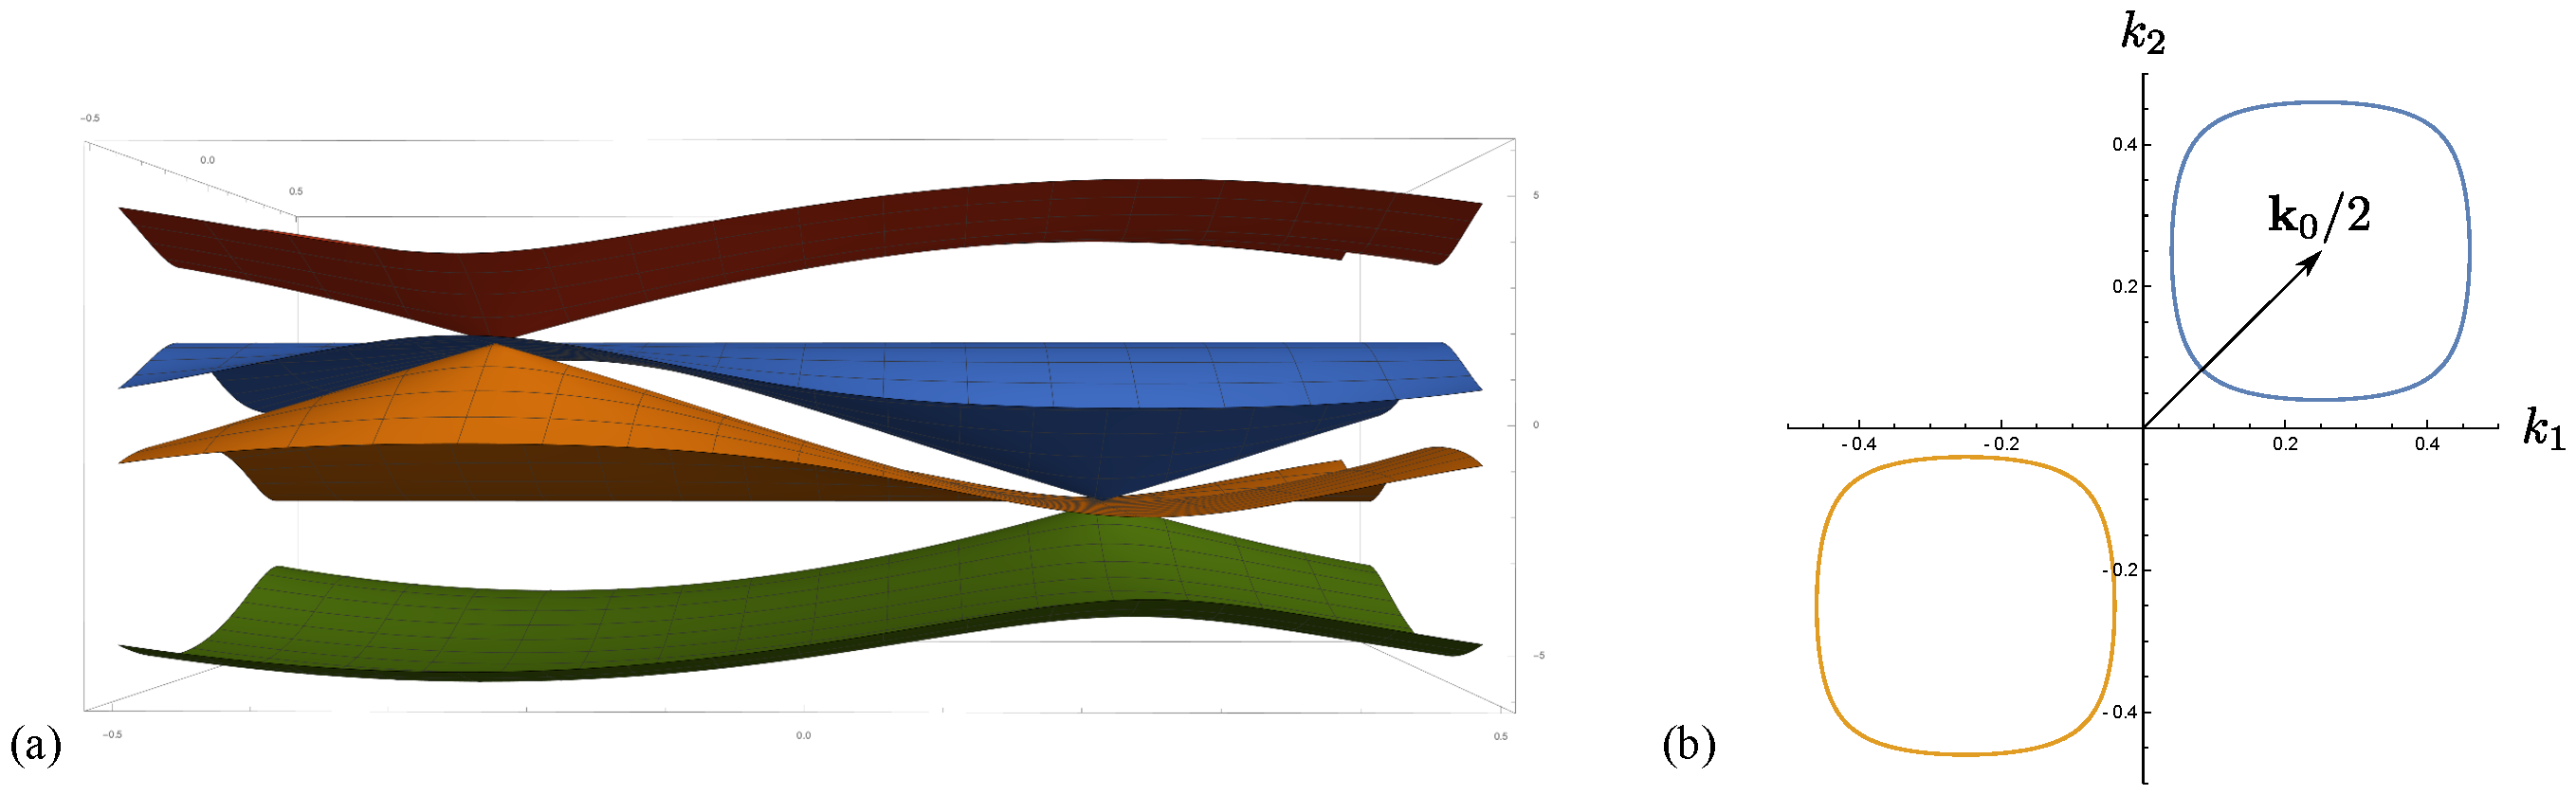
\includegraphics[width=\linewidth]{./chapter07/SquareOctagonPanel1.pdf}
	\caption{
		(a) Gapless band structure of the Kitaev model on the square-octagon lattice.
		(b) Nodal lines of the Kitaev model on the square-octagon lattice.
	}
	\label{fig:chapter07_SquareOctagonPanel1}
\end{figure}
%

There are essentially two types of terms to calculate: those for which both fermions come from either above or below the Fermi level (referred to below as particle-particle or hole-hole terms, respectively), \ie,
%
\begin{equation}
	\propto e^{i (\bp^* + \bq^*) \cdot \br} \avg{f_{FS}(\bp^* + \bp) f\dag_{FS}(\bp^* + \bp)} \avg{f_{FS}(\bq^* + \bq) f\dag_{FS}(\bq^* + \bq)},
\end{equation}
%
and those for which one fermion comes from above (below) the Fermi level while the other comes from below (above) the Fermi level (referred to below as particle-hole or hole-particle terms, respectively), \ie,
%
\begin{equation}
	\propto e^{i (\bp^* - \bq^*) \cdot \br} \avg{f_{FS}(\bp^* + \bp) f\dag_{FS}(\bp^* + \bp)} \avg{f\dag_{FS}(\bq^* + \bq) f_{FS}(\bq^* + \bq)}.
\end{equation}
%

For the determination of Friedel oscillations one additionally needs the values of $\bp^*$ and $\bq^*$.
The first case to consider is $\bp^* = \bq^*$.
For particle-hole terms which have prefactor $e^{i(\bp^* - \bq^*)\cdot\br}$, there are no oscillations.
However, particle-particle terms which have prefactor $e^{i(\bp^* + \bq^*)\cdot\br}$ generate oscillations with wavevector $\bk = 2\bk_F(\bp^*) + \bk_0$, where $\bk_F(\bp^*) = \bp^* - \bk_0/2$ (refer to Figure~\ref{fig:chapter07_SquareOctagonPanel1}~(b)).
Friedel oscillations for hole-particle or hole-hole terms are determined in the same manner.

Next consider the role of time-reversal symmetry which maps $\bq \mapsto -\bq + \bk_0$ and take $\bp^*, \bq^*$ to be time-reversal pairs, \ie, $\bq^* = -\bp^* + \bk_0$.
For particle-hole terms which have prefactor $e^{i(\bp^* - \bq^*)\cdot\br}$, there will be oscillations with wavevector $\bk = 2\bk_F(\bp^*)$.
Particle-particle terms which have prefactor $e^{i(\bp^* + \bq^*)\cdot\br}$ generate oscillations with wavevector $\bk = \bk_0$.
Again, the Friedel oscillations for hole-particle or hole-hole terms are determined in the same manner.

At these wavevectors one can expect singular behavior in the Fourier transform of the bond-bond correlation function resulting in an algebraic decay in real space.
In order to determine the manner in which the correlation function decays, one must calculate the asymptotic behavior of the integrals of Eq.~\eqref{eq:chapter07_TwoPointAsymptotic}.
Since the wave function terms $\chi_{FS}$ are smooth and non-vanishing at the Fermi level, they will be approximated as constants and replaced by their value at the corresponding points $\bp^*, \bq^*$.
The long distance behavior then comes from the sharp cutoff of the Green's functions at the Fermi level.

To calculate this, the quasiparticle energy is expanded about the points $\bp^*, \bq^*$ as, \eg,
%
\begin{equation}
	\epsilon(\bp^* + \bp) = v_F \left( \zeta p_{\parallel} + \frac{\alpha}{2} p_{\bot}^2 \right),
\end{equation}
%
where $p_{\parallel}$ and $p_{\bot}$ are the components of $\bp$ parallel and perpendicular to $\br$, respectively, $v_F$ and $\alpha$ are the Fermi velocity and curvature of the Fermi surface at the point $\bp^*$, respectively, and $\zeta = \pm 1$ depending on whether the fermion is right or left moving at the point $\bp^*$.
Using this approximation, the real-space Green's functions may be calculated, \eg, for a right-moving fermion as
%
\begin{align}
	&\int d^2p~ e^{i\bp\cdot\br} \avg{f_{FS}(\bp) f\dag_{FS}(\bp)} = \int dp_{\parallel} e^{i p_{\parallel} r} \int dp_{\bot}~ H(\epsilon(\bp^* + \bp)) \nonumber\\
	&\qquad\approx \int_{-\infty}^{\infty} dp_{\parallel} e^{i p_{\parallel} r} H(-p_{\parallel})\Bigg[\int_{-\Lambda}^{-\sqrt{-2p_{\parallel}/\alpha}} dp_{\bot} + \int_{\sqrt{-2p_{\parallel}/\alpha}}^{\Lambda} dp_{\bot}\Bigg] \nonumber\\
	&\qquad\qquad+ \int_{-\infty}^{\infty} dp_{\parallel}~ e^{i p_{\parallel} r} H(p_{\parallel}) \int_{-\Lambda}^{\Lambda} dp_{\bot},
\end{align}
%
where $H(x)$ is the Heaviside step function and $\Lambda$ is an arbitrary momentum cutoff which does not affect the final result.
Only the first two terms contribute to the long-wavelength behavior of the correlation function and may be evaluated as~\cite{Lighthill1958}
%
\begin{align}
	\int d^2p~ e^{i\bp\cdot\br} \avg{f_{FS}(\bp) f\dag_{FS}(\bp)} &\approx -2\sqrt{\frac{2}{\alpha}} \int_{-\infty}^{\infty} dp_{\parallel} e^{i p_{\parallel} r} \abs{p_{\parallel}}^{1/2} H(-p_{\parallel}) \nonumber\\
	&= -\sqrt{\frac{2\pi}{\alpha}} \frac{e^{-i 3\pi/4}}{r^{3/2}}.
\end{align}
%
The remainder of the real-space Green's functions may be evaluated similarly yielding
%
\begin{align}
	\int d^2p~ e^{i\bp\cdot\br} \avg{f_{FS}(\bp) f\dag_{FS}(\bp)} &\approx -\sqrt{\frac{2\pi}{\alpha}} \frac{e^{-\zeta i 3\pi/4}}{r^{3/2}} \nonumber\\
	\int d^2p~ e^{-i\bp\cdot\br} \avg{f\dag_{FS}(\bp) f_{FS}(\bp)} &\approx \sqrt{\frac{2\pi}{\alpha}} \frac{e^{\zeta i 3\pi/4}}{r^{3/2}},
\end{align}
%
where $\zeta = \pm 1$ for $\bp^*$ corresponding to right- and left-moving fermions, respectively.
%
\begin{figure}[tb]
	\centering
	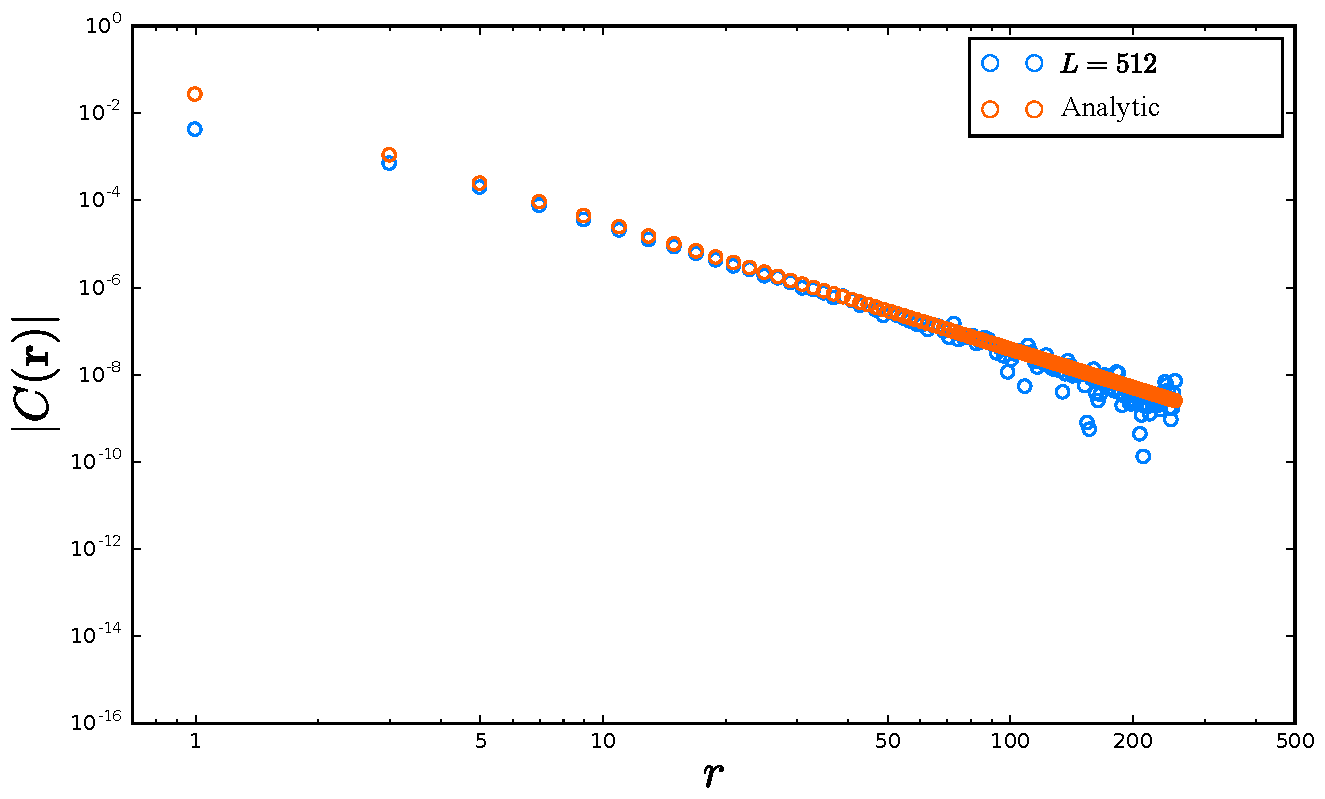
\includegraphics[width=0.8\linewidth]{./chapter07/SquareOctagonPanel2.pdf}
	\caption{
		Comparison of numerics and analytics for bond-bond correlations on the square-octagon lattice for $\br = r \ba_1$.
	}
	\label{fig:chapter07_SquareOctagonPanel2}
\end{figure}
%

The final analytic expression for the bond-bond correlation function must contain terms from all combinations of $\bp^*$ and $\bq^*$ and is rather lengthy, however, it can already be seen from here that the correlations will decay as a power law $C(\br) \sim 1/r^3$.
Using numerically obtained values for $\alpha$, $\bp^*$, $\bq^*$ and the wave functions, Figure~\ref{fig:chapter07_SquareOctagonPanel2} shows a comparison of the asymptotic expression derived above to the numerically obtained data discussed in Section~\ref{section:chapter07_BondBondGeneral} for $\br = r \ba_1$, where $\ba_1$ is a lattice vector of the square-octagon lattice.
Other than finite size effects for larger values of $r$, the asymptotic expression yields a very good fit to the data.
One can see in the figure that bond-bond correlations vanish entirely for even values of $r$ due to the perfect nesting vector $\bk_0$, as the bond-bond correlation function in the $\ba_1$-direction takes the general form
%
\begin{equation}
	C(\br) \propto \frac{1 - \cos{(\bk_0 \cdot \br)}}{r^3} = \frac{1 - \cos{(\pi r)}}{r^3}.
\end{equation}
%


%
%
%%%%%%%%%%%%%%%%%%%%%%%%%%%%%%%%%%%%%%%%%%%%%%%%%%%%%%%%%%%%%%%%%%%%%%%%%%%%%%%%%%%%%%%%
\subsubsection{Honeycomb lattice}
\label{section:chapter07_BondBondHoneycomb}
%%%%%%%%%%%%%%%%%%%%%%%%%%%%%%%%%%%%%%%%%%%%%%%%%%%%%%%%%%%%%%%%%%%%%%%%%%%%%%%%%%%%%%%%
%
%
As already mentioned in this thesis, the gapless Kitaev spin liquid on the honeycomb lattice hosts two Dirac nodes corresponding to two linearly-dispersing bands as pictured in Figure~\ref{fig:chapter07_HoneycombDispersion}.
In the following, the convention is used such that fermionic creation operators $f\dag$ correspond to the band which is colored blue in the figure.
This band touches the Fermi level at two Dirac nodes located at $\pm \bk_{\rm Dirac} = \pm (\bq_1 - \bq_2)/3$.
As all states lie below the Fermi level, the only non-vanishing terms contributing to the bond-bond correlation functions are the hole-hole terms, \ie,
%
\begin{equation}
	\propto e^{-i (\bp^* + \bq^*) \cdot \br} \avg{f\dag_{FS}(\bp^* + \bp) f_{FS}(\bp^* + \bp)} \avg{f\dag_{FS}(\bq^* + \bq) f_{FS}(\bq^* + \bq)}.
\end{equation}
%
%
\begin{figure}[tb]
	\centering
	\includegraphics[width=0.9\linewidth]{./chapter07/HoneycombDispersion.pdf}
	\caption{
		Gapless Dirac cone band structure of the Kitaev model on the honeycomb lattice.
	}
	\label{fig:chapter07_HoneycombDispersion}
\end{figure}
%

For the determination of Friedel oscillations one additionally needs the values of $\bp^*$ and $\bq^*$.
For the honeycomb lattice there are only two such points, \ie, the locations of the Dirac nodes.
The first case to consider is $\bp^* = \bq^*$.
Hole-hole terms which have prefactor $e^{-i(\bp^* + \bq^*)\cdot\br}$ will generate oscillations with wavevector $\bk = \pm 2\bk_{\rm Dirac}$.
Next, consider the role of time-reversal symmetry which maps $\bq \mapsto -\bq$.
For time-reversal pairs $\bq^* = -\bp^*$, hole-hole terms with prefactor $e^{-i(\bp^* + \bq^*)\cdot\br}$ do not result in Friedel oscillations, \ie, $\bk = \bz$.

At these wavevectors one can expect singular behavior in the Fourier transform of the bond-bond correlation function resulting in an algebraic decay in real space.
The Green's functions are equal to unity for all momenta due to the semi-metallic nature of the fermion dispersion, therefore, the algebraic correlations come from the non-analyticity of the wave functions at the Dirac nodes.
Terms such as $\chi_{FS}^{AA}$ and $\chi_{FS}^{BB}$ are constant for all momenta and, thus, do not contribute to the long-wavelength behavior of the correlation function.
In this case, the relevant expression for the asymptotic bond-bond correlation function is given by
%
\begin{equation}
	C(\br) \sim -\frac{4}{(2\pi)^4} \sum_{\bp^*, \bq^*} e^{-i(\bp^* + \bq^*)\cdot\br} \int d^2p~d^2q~ e^{-i(\bp + \bq)\cdot\br} \chi_{FS}^{AB}(\bp^* + \bp) \chi_{FS}^{BA}(\bq^* + \bq).
\end{equation}
%
Setting $J_x = J_y = (1 - J_z)/2$, expanding the wave functions about the Dirac nodes and summing over $\bp^*$ and $\bq^*$, one arrives at an expression for the correlation function
%
\begin{align}
	C(\br) &\sim -\frac{4}{(2\pi)^4} \int d^2p~d^2q~ e^{-i(\bp + \bq)\cdot\br}~\times \nonumber\\
	&\qquad\Bigg\{ 2\cos{(2\bk_{\rm Dirac}\cdot\br)}\left[A^2 - B^2 + C^2 - D^2 + 2CE + E^2 - 2DF - F^2\right] \nonumber\\
	&\qquad\phantom{\Bigg\{}+ 4i\sin{(2\bk_{\rm Dirac}\cdot\br)}\left[-AC + BD - AE + BF\right] \nonumber\\
	&\qquad\phantom{\Bigg\{}+ 2\left[A^2 + B^2 - C^2 - D^2 - 2CE - E^2 - 2DF - F^2\right]\Bigg\},
\end{align}
%
where
%
\begin{equation}
	\begin{matrix*}[l]
		A = -\dfrac{v_y p_y}{2\sqrt{v_x^2 p_x^2 + v_y^2 p_y^2}}, &
		B = i\dfrac{v_x p_x}{2\sqrt{v_x^2 p_x^2 + v_y^2 p_y^2}}, \\
		&\\
		C = -\dfrac{3 \alpha J_z v_x^3 v_y p_x^3 p_y}{8(v_x^2 p_x^2 + v_y^2 p_y^2)^{3/2}}, &
		D = -i\dfrac{3 \alpha J_z v_x^2 v_y^2 p_x^2 p_y^2}{8(v_x^2 p_x^2 + v_y^2 p_y^2)^{3/2}}, \\
		&\\
		E = -\dfrac{v_x v_y^3 p_x p_y^3}{8 J_z (v_x^2 p_x^2 + v_y^2 p_y^2)^{3/2}}, &
		F = -i\dfrac{v_y^4 p_y^4}{8 J_z (v_x^2 p_x^2 + v_y^2 p_y^2)^{3/2}},
	\end{matrix*}
\end{equation}
%
and with
%
\begin{equation}
	\begin{matrix*}[l]
		v_x = \sqrt{1 - 2J_z},	& \qquad\qquad	& v_y = \sqrt{3} J_z,	\\
		\\
		\alpha = J_z \left(\frac{1}{3 v_x^2} + \frac{2}{v_y^2}\right),	& \qquad\qquad	& \bk_{\rm Dirac} = \frac{1}{2\pi} \arccos{\left(-\frac{J_z}{1 - J_z}\right)} (\bq_1 - \bq_2).
	\end{matrix*}
\end{equation}
%

One may now choose a direction for $\br$ and evaluate the integrals analogously to what was done for the square-octagon lattice above~\cite{Lighthill1958}.
For $\br = r(\ba_1 + \ba_2)$ there are no Friedel oscillations due to $2\bk_{\rm Dirac}\cdot\br = 0$.
The bond-bond correlations for the $(\ba_1 + \ba_2)$-direction may be evaluated as
%
\begin{equation}
	C(\br) \sim \frac{v_y^2}{v_x^2}\frac{1}{9\pi^2 r^4}.
\end{equation}
%
Comparing to the numerical data in Figure~\ref{fig:chapter07_HoneycombPanel}, the asymptotic expression above provides a good fit, reproducing the $1/r^4$ behavior seen in Section~\ref{section:chapter07_BondBondGeneral}.
As the exchange couplings are tuned within the gapless phase, only the overall prefactor of the correlations changes.

The bond-bond correlations are more complicated for $\br = r(\ba_1 - \ba_2)$.
In this case the correlation function may be evaluated as
%
\begin{align}
	C(\br) \sim &-\frac{v_x^2}{2\pi^2 v_y^2} \left[1 - \cos{(2\bk_{\rm Dirac}\cdot\br)}\right] \frac{1}{r^4} \nonumber\\
	&-\frac{3 v_x^3 (1 - 2\alpha J_z)}{4\pi^2 J_z v_y^2} \sin{(2\bk_{\rm Dirac}\cdot\br)} \frac{1}{r^5} \nonumber\\
	&-\frac{9 v_x^4 (1 - 2\alpha J_z)^2}{32 \pi^2 J_z^2 v_y^2} \left[1 + \cos{(2\bk_{\rm Dirac}\cdot\br)}\right] \frac{1}{r^6}.
\end{align}
%
Comparing to the numerical data in Figure~\ref{fig:chapter07_HoneycombPanel}, the asymptotic expression above provides a good fit.
At the isotropic point one sees that the $1/r^4$ term dominates for $r \neq 0~({\rm mod}~3)$, whereas the $1/r^6$ term dominates for $r = 0~({\rm mod}~3)$ due to an exact cancellation of the leading order term from Friedel oscillations.
Away from the isotropic point where $2\bk_{\rm Dirac}\cdot\br \neq 0~({\rm mod}~2\pi)$ for integer $r$, there is a complex interplay of all three terms.
Using the asymptotic analysis here, even this more complex behavior is captured.
%
\begin{figure}[tb]
	\centering
	\includegraphics[width=\linewidth]{./chapter07/HoneycombPanel.pdf}
	\caption{
		Comparison of numerics and analytics for bond-bond correlations on the honeycomb lattice for (left) $\br = r (\ba_1 + \ba_2)$ and (right) $\br = r (\ba_1 - \ba_2)$ with $J_x = J_y = (1 - J_z)/2$ for (top) $J_z > J_x, J_y$, (middle) $J_z = J_x = J_y$ and (bottom) $J_z < J_x, J_y$.
	}
	\label{fig:chapter07_HoneycombPanel}
\end{figure}
%


%
%
%%%%%%%%%%%%%%%%%%%%%%%%%%%%%%%%%%%%%%%%%%%%%%%%%%%%%%%%%%%%%%%%%%%%%%%%%%%%%%%%%%%%%%%%
\subsubsection{Three-dimensional lattices}
\label{section:chapter07_BondBondThreeDimensions}
%%%%%%%%%%%%%%%%%%%%%%%%%%%%%%%%%%%%%%%%%%%%%%%%%%%%%%%%%%%%%%%%%%%%%%%%%%%%%%%%%%%%%%%%
%
%
While a thorough investigation of the asymptotic behavior of the bond-bond correlation function has not been performed for the three-dimensional lattices, some general remarks may be made.
The simplest case to study is for fully two-dimensional Fermi surfaces as in lattice (10,3)a.
Similar to the nodal line in \textit{two}-dimensions, the algebraic decay comes from the sharp cutoff of the momentum-space fermion Green's functions at the Fermi level.
For the Fermi surface in three-dimensions, the fermion Green's functions take the form~\cite{Lighthill1958}, \eg,
%
\begin{align}
	\int d^3p~ e^{i\bp\cdot\br} \avg{f_{FS}(\bp) f\dag_{FS}(\bp)} &\sim \frac{2}{\sqrt{\alpha}} \int_{-\infty}^{\infty} dp_{\parallel}~ e^{i p_{\parallel} r} \abs{p_{\parallel}} H(-p_{\parallel}) \nonumber\\
	&\sim \frac{1}{r^2},
\end{align}
%
yielding a bond-bond correlation function which decays as $C(\br) \sim 1/r^4$, as is seen in the numerical data of Section~\ref{section:chapter07_BondBondGeneral}.

The semi-metallic cases of Fermi lines and Weyl nodes in three-dimensions are more complicated as the algebraic correlations come from the non-analyticity of the fermion wave functions rather than from the Green's functions.
As one does not have access to an analytic expression for the wave functions here as opposed to the case of the two-dimensional Dirac nodes, one must resort to idealized wave functions for the two cases.
This analysis has not been performed, but some general remarks and speculation will be made.

For the Fermi line in three-dimensions, one might assume a wave function of the same form as the Dirac nodes in the last section, where $p_x$ and $p_y$ now correspond to two directions orthogonal to the Fermi line.
For the direction tangent to the Fermi line, the wave function should be well-behaved and not contribute anything additional to the long-wavelength behavior of the correlation functions.
In this idealized case, one would expect correlations to decay as $C(\br) \sim 1/r^4$ just as for the Dirac nodes in two-dimensions.
For observation directions $\br$ \textit{orthogonal} to the plane in which the Fermi line lies and where all points on the Fermi line contribute, this is indeed the behavior seen in the numerics presented in Section~\ref{section:chapter07_BondBondGeneral}.
The author speculates that for the observation directions $\br$ \textit{parallel} to the plane in which the Fermi line lies, the observed $1/r^5$ decay is due to a cancellation of the leading order $1/r^4$ term similar to what was seen to occur for the Dirac nodes.

Finally, the author has not performed an analysis for the case of the Weyl nodes in three-dimensions, but imagines that the calculation of the decay envelope may be performed straightforwardly by assuming an idealized wave function for a Weyl node similar to what was described for the Fermi line above.


%
%
%%%%%%%%%%%%%%%%%%%%%%%%%%%%%%%%%%%%%%%%%%%%%%%%%%%%%%%%%%%%%%%%%%%%%%%%%%%%%%%%%%%%%%%%
\section{Bond-bond correlations at finite temperature}
\label{section:chapter07_BondBondCorrelationsFiniteTemperature}
%%%%%%%%%%%%%%%%%%%%%%%%%%%%%%%%%%%%%%%%%%%%%%%%%%%%%%%%%%%%%%%%%%%%%%%%%%%%%%%%%%%%%%%%
%
%
As was done for the nearest-neighbor spin-spin correlations in Section~\ref{section:chapter07_SpinSpinCorrelationsFiniteTemperature}, one may similarly ask what is the fate of the bond-bond correlation function at finite temperature.
In order to calculate the thermal bond-bond correlation function, one needs to evaluate thermal expectation values of products of Majorana two-point functions of the form
%
\begin{equation}
	\avg{\avg{c_i c_j}\avg{c_k c_l}}_{T} = \frac{1}{Z} \sum_{\{n_\alpha\}_{\alpha=1}^N} \avg{c_i c_j}_{\{n_\alpha\}} \avg{c_k c_l}_{\{n_\alpha\}} \exp{\left[-\beta \sum_{\lambda=1}^N \epsilon_\lambda (n_\lambda - 1/2)\right]},
\end{equation}
%
where, once again, fermionic creation operators $f\dag$ are chosen to correspond to the single-particle states with non-negative energy.
The many-particle trace may be simplified as
%
\begin{align}
	\avg{\avg{c_i c_j}\avg{c_k c_l}}_{T} 	&= \frac{4}{Z} \sum_{\{n_\alpha\}_{\alpha=1}^N} \sum_{\mu,\nu=1}^N (-1)^{n_\mu+n_\nu} \chi^{ij}_\mu \chi^{kl}_\nu \prod_{\lambda=1}^N \exp{\Big[(-1)^{n_\lambda} \Theta_\lambda \Big]} \nonumber\\
	&= 4 \sum_{\mu,\nu=1}^N \chi^{ij}_\mu \chi^{kl}_\nu \Big[ (1-\delta_{\mu,\nu}) \tanh{[\Theta_\mu]} \tanh{[\Theta_\nu]} + \delta_{\mu,\nu} \Big].
\end{align}
%
Using the above expression, the bond-bond correlation function at finite temperature may be expressed in a fixed gauge as
%
\begin{align}
	\avg{C(\bR)}_T	&= -\frac{4}{V} \sum_{\bR'} u_{AB}(\bR') u_{AB}(\bR' + \bR)~\times \nonumber\\
	&\qquad\sum_{\mu,\nu} \Bigg[\Big(\psi_{\mu}^A(\bR') \overline{\psi}_{\mu}^A(\bR' + \bR)\Big) \Big(\psi_{\nu}^B(\bR' + \bR) \overline{\psi}_{\nu}^B(\bR') \Big) \nonumber\\
	&\qquad\qquad+ \Big(\psi_{\mu}^A(\bR') \overline{\psi}_{\nu}^A(\bR' + \bR)\Big) \Big(\psi_{\nu}^B(\bR') \overline{\psi}_{\mu}^B(\bR' + \bR) \Big)\Bigg]~\times \nonumber\\
	&\qquad\Big[(1-\delta_{\mu,\nu})\tanh{[\beta \epsilon_\mu/2]}\tanh{[\beta \epsilon_\nu/2]} + \delta_{\mu,\nu} \Big].
\end{align}
%
For a translationally invariant gauge configuration this may be evaluated in momentum space as
%
\begin{align}
	\tilde{C}(\bk, T) &= -\frac{4}{V^{3/2}} \sum_{\bq} \sum_{\alpha,\beta} \Bigg[ \left|\psi_{\alpha}^A(\bk + \bq)\right|^2 \left|\psi_{\beta}^B(\bq)\right|^2 \nonumber\\
	&\qquad\qquad\qquad+ \left(\psi_{\alpha}^A(\bk + \bq) \overline{\psi}_{\beta}^A(\bq)\right) \left(\psi_{\beta}^B(\bq) \overline{\psi}_{\alpha}^B(\bk + \bq)\right) \Bigg]~\times \nonumber\\
								&\qquad\Bigg[ (1 - \delta_{\bk,\bm{0}}\delta_{\alpha,\beta}) \tanh{\left(\beta \epsilon_\alpha(\bk+\bq)/2\right)} \tanh{\left(\beta \epsilon_\beta(\bq)/2\right)} + \delta_{\bk,\bm{0}}\delta_{\alpha,\beta} \Bigg],
\end{align}
%
where $\alpha,\beta$ are band indices.

For $T\rightarrow 0$ one recovers the ground state bond-bond correlation function from the previous section, whereas for $T\rightarrow \infty$ the correlation function becomes
%
\begin{align}
	\avg{C(\bR)}_T	&= -\frac{4}{V} \sum_{\bR'} u_{AB}(\bR') u_{AB}(\bR' + \bR)~\times \nonumber\\
					&\qquad\sum_{\mu} \Bigg[\Big(\psi_{\mu}^A(\bR') \overline{\psi}_{\mu}^A(\bR' + \bR)\Big) \Big(\psi_{\mu}^B(\bR' + \bR) \overline{\psi}_{\mu}^B(\bR') \Big) \nonumber\\
					&\qquad\qquad+ \Big(\psi_{\mu}^A(\bR') \overline{\psi}_{\mu}^A(\bR' + \bR)\Big) \Big(\psi_{\mu}^B(\bR') \overline{\psi}_{\mu}^B(\bR' + \bR) \Big)\Bigg].
\end{align}
%
For a translationally invariant gauge configuration this may be evaluated in momentum space as

%
\begin{equation}
	C(\bR, T\rightarrow\infty) = -\frac{8}{V^2} \sum_{\bq} \sum_{\alpha} \left|\psi_{\alpha}^A(\bq) \right|^2 \left|\psi_{\alpha}^B(\bq) \right|^2.
\end{equation}
%
From here it is obvious that for any translationally invariant gauge, bond-bond correlations should vanish as $1/V^2$.
Figure~\ref{fig:chapter07_6_3BondBondHighTemp} shows the bond-bond correlation function times squared system size calculated numerically for a number of system sizes on the honeycomb lattice in the ground state flux sector and at a temperature roughly ten times the exchange couplings.
Here it can be seen that the bond-bond correlation function indeed vanishes as $1/V^2$.
%
\begin{figure}[tb]
	\centering
	\includegraphics[width=0.8\linewidth]{./chapter07/HoneycombBondBondT=10.pdf}
	\caption{
		High-temperature bond-bond correlation function times squared system size calculated numerically for a number of system sizes on the honeycomb lattice in the ground state flux sector.
	}
	\label{fig:chapter07_6_3BondBondHighTemp}
\end{figure}
%

This analysis, of course, has ignored the thermal fluctuations of the gauge field for simplicity.
The author speculates that the $T \rightarrow \infty$ limit still holds for an arbitrary gauge configuration, however, in order to properly investigate the fate of bond-bond correlations at finite temperatures, one must include these fluctuations.


%
%
%%%%%%%%%%%%%%%%%%%%%%%%%%%%%%%%%%%%%%%%%%%%%%%%%%%%%%%%%%%%%%%%%%%%%%%%%%%%%%%%%%%%%%%%
\section{Summary and outlook}
\label{section:chapter07_Summary}
%%%%%%%%%%%%%%%%%%%%%%%%%%%%%%%%%%%%%%%%%%%%%%%%%%%%%%%%%%%%%%%%%%%%%%%%%%%%%%%%%%%%%%%%
%
%
The work reported in this chapter is the subject of ongoing study and, thus, leaves several questions open without unequivocal answers.
There are, however, a number of successes reported here as well.
This chapter began with a recapitulation of some well-known results about the Kitaev model for classical $O(3)$ spins.
In the classical model, the ground state manifold corresponds to an extensively degenerate number of dimer configurations where each spin is perfectly aligned with one of its nearest-neighbors.
The resulting classical spin liquid phase yields spin-spin correlations which vanish beyond nearest-neighbor spins due to the disordered nature of the dimer configurations.
By mapping to a hardcore dimer model and then to a coarse-grained field theory, the ground state manifold has been shown to be in a so-called Coulomb phase.
Thus it is argued on rather general grounds that bond-bond correlations in the classical Kitaev model should decay as a power law $C(\br) \sim 1/r^D$, where $D$ is the dimension of the lattice.

In the quantum model, spin-spin correlations similarly vanish beyond nearest-neighbors due to the conservation of \ZZ~fluxes.
Furthermore, the bond-bond correlation function also decays algebraically so long as the system is in a gapless spin liquid phase, otherwise it decays exponentially.
Rather than depending only on the dimension of the underlying lattice as is the case for the classical model, the decay exponent of the quantum model also depends intimately on the nature of the gapless excitations of the spin liquid.
A general trend is observed that the greater the dimension of the nodal manifold, the slower the decay of correlations.

Bond-bond correlations were calculated numerically for a number of both two- and three-dimensional lattices.
Additionally, the bond-bond correlation function was evaluated analytically in the long-wavelength limit for both the square-octagon and honeycomb lattices, showing good agreement with the numerics.
Although a detailed analysis has not yet been performed for the three-dimensional lattices, knowledge from the analysis of the two-dimensional lattices allowed for some general remarks to be made which are in qualitative agreement with the numerical data.	% Correlations in Kitaev Spin Liquids
%%%%%%%%%%%%%%%%%%%%%%%%%%%%%%%%%%%%%%%%%%%%%%%%%%%%%%%%%%%%%%%%%%%%%%%%%%%%%%%%%%%%%%%%
\chapter{Summary and Outlook}
\label{chapter:Conclusion}
%%%%%%%%%%%%%%%%%%%%%%%%%%%%%%%%%%%%%%%%%%%%%%%%%%%%%%%%%%%%%%%%%%%%%%%%%%%%%%%%%%%%%%%%
%
%
In this thesis a number of three-dimensional tricoordinated lattices were introduced for which the Kitaev honeycomb model could be defined while retaining its exact solvability.
In doing so, a variety of novel gapless \ZZ~spin liquid states were revealed.
The gapless fermionic quasiparticle excitations occurring in these spin liquids vary greatly depending on the underlying lattice, ranging from fully two-dimensional Fermi surfaces and nodal lines protected by winding numbers of different dimension, to point-like topological degeneracies analogous to the Weyl fermion of high-energy theory.

Alongside a detailed analysis of the various three-dimensional gapless spin liquid phases, the concepts of quantum order and the projective symmetry group were utilized to deduce general constraints on the gapless excitations, thereby providing a classification scheme for the gapless Kitaev spin liquids.
A further investigation was undertaken to map the significantly more complicated ground state phase diagram for the non-bipartite lattice (9,3)a which was seen to host a number of both gapped and gapless \textit{chiral} spin liquid phases.
Finally, first results from a study of correlations in Kitaev spin liquids were reported.
Here it was seen how the various Fermi surface topologies of the gapless quasiparticles influence the algebraic correlations of certain four-spin correlation functions.

Beyond the obvious conclusion of the work on algebraic correlations in the Kitaev spin liquids, there are a number of interesting avenues for further study one might consider.
Already, the Kitaev model for several of the lattices introduced in this work have been studied via quantum Monte Carlo simulation~\cite{YasuyukiPRB2017,EschmannPRL2019} as well as in the context of potential experimental signatures via Raman spectroscopy~\cite{PerreaultPRB2016a,PerreaultPRB2016b} and resonant inelastic x-ray scattering~\cite{HalaszPRL2017}.

Whereas the work presented in this thesis focuses heavily on the gapless Kitaev spin liquids, a thorough investigation of the \textit{gapped} spin liquids might also be promising.
It has long been known that the gapped spin liquid phase of Kitaev's original model on the honeycomb lattice is equivalent to the toric code model and hosts exotic Abelian anyon quasiparticles~\cite{KitaevAoP2006}.
A study of the gapped spin liquid phase for the hyperhoneycomb lattice~\cite{MandalPRB2014} uncovered loop-like excitations obeying fermionic statistics.
Furthermore, it was shown that a fermionic loop braided through a larger loop excitation acquires a non-trivial phase.
In Appendix~\ref{appendix:LoopModels} a number of effective loop models were derived for the gapped three-dimensional Kitaev spin liquids, however, the nature of their excitations remains an open question.

Finally, one might investigate the role of disorder in three-dimensional Kitaev spin liquids.
One potential source of disorder is the inclusion of vacancies.
In fact, isolated (and pairs of) vacancies have been studied before for Kitaev spin liquids on the honeycomb~\cite{WillansPRL2010,WillansPRB2011,SanthoshPRB2012,HalaszPRB2014} and hyperhoneycomb~\cite{SreejithPRB2016} lattices.
On the two-dimensional honeycomb lattice it was shown that a single vacancy binds a flux and induces a local moment.
In the gapped phase this moment is free, whereas in the gapless phase the low-field vacancy magnetization is given by $m(h) \sim h \ln{(1/h)}$, where $h$ is a weak, applied magnetic field.
For the three-dimensional hyperhoneycomb lattice it was found that, while a vacancy does not bind a \ZZ~flux, it similarly induces a local moment.
The local moment is again free in the gapped phase, however, in the gapless phase the low-field vacancy magnetization is now given by $m(h) \sim 1/\sqrt{\ln{(1/h)}}$.
As it is the interaction of the vacancy moment with the surrounding gapless spin liquid which suppresses the magnetization, it would be interesting to explore this problem on other three-dimensional lattices which host qualitatively different nodal manifolds.

Another particularly interesting line of investigation is on the effects of Gaussian spatially-correlated disorder of the exchange couplings in the Weyl spin liquids.
A similar situation has been explored in the Weyl \textit{semi-metals} with a correlated on-site disorder potential.
The resulting physics is seen to be a function of both disorder strength and the correlation length $\xi$ of the disorder potential.
The natural length scale $\lambda$ determined by the momentum-space distance between Weyl nodes allows one to distinguish between disorder with and without substantial backscattering, corresponding to $\xi \ll \lambda$ and $\xi \gtrsim \lambda$, respectively.

For disordered Weyl semi-metals without backscattering and a sufficiently short-ranged random potential, renormalization group calculations~\cite{SyzranovPRB2015} indicate a phase transition from the Weyl semi-metal to a diffusive metal occurs at a finite critical disorder strength.
In this case, the disorder-averaged density of states may be used as an order-parameter for the transition.
Weak disorder is seen to be irrelevant and only renormalizes the Fermi velocity, leaving the quadratic scaling of the density of states intact.
In the vicinity of the transition, the density of states scales linearly with the absolute value of the energy before the system is driven into the diffusive metal phase with a finite density of states.
Missing from the above analysis, however, are the effects of rare-regions in the disorder potential.
Quasilocalized states due to rare, but strong fluctuations of the disorder potential lead to an exponentially small density of states resulting in an avoided quantum critical point~\cite{NandkishorePRB2014,PixleyPRX2016}.
Although these rare-region effects round out the non-analyticity for the smallest energies, the critical scaling can still be observed for sufficiently large energies.

For systems without backscattering and an extremely slowly-varying Gaussian random potential, the system undergoes a transition from a Weyl semi-metal to a diffusive metal at a finite disorder strength and the criticality is controlled by a long-ranged fixed point~\cite{LouvetPRB2017}.
The physical consequences of this fixed point have yet to be explored, however, it is likely that the critical behavior of the density of states is rounded out by rare-region effects as in the case of short-ranged disorder.

For the case of ultra-short-ranged disorder where significant backscattering couples different Weyl nodes, it has been argued that the same results from the analysis of \textit{decoupled} Weyl points with a short-ranged potential still apply for sufficiently weak disorder strengths, \ie, the system undergoes a transition from a Weyl semi-metal to a diffusive metal at some finite critical disorder strength~\cite{PixleyPRB2017}.
However, for even stronger disorder, strong backscattering between Weyl points drives the system through an Anderson localization transition~\cite{PixleyPRL2015}.

An interesting question is how the physics of disordered Weyl \textit{spin liquids} might differ.
As the Weyl spin liquids fall into different Altland-Zirnbauer symmetry classes than the Weyl semi-metals, it is not unreasonable to expect the spin liquids to be affected differently by disorder.
There are also the effects of the \ZZ~gauge field to consider.
On the one hand, sign changes in hopping strengths of the Majoranas may be gauged away for sufficiently weak disorder.
On the other hand, strong disorder may drive the ground state into more complex flux sectors, significantly complicating such a study.	% Summary and Outlook


%%%%%%%%%%%%%%%%%%%%%%%%%%%%%%%%%%%%%%%%%%%%%%%%%%%%%%%%%%%%%%%%%
% BACK MATTER
%%%%%%%%%%%%%%%%%%%%%%%%%%%%%%%%%%%%%%%%%%%%%%%%%%%%%%%%%%%%%%%%%
%
%
\newpage
\mbox{}
\newpage
\appendix
\part*{Appendices}
\addcontentsline{toc}{part}{Appendices}
\pagestyle{empty}
\pagestyle{fancy}
\fancyhead{}
\setlength{\headheight}{13.6pt}
\fancyhead[RE]{\nouppercase\leftmark}
\fancyhead[LE]{\textbf{\thepage}}
\fancyhead[LO]{\nouppercase\rightmark}
\fancyhead[RO]{\textbf{\thepage}}
\cfoot{}


%%%%%%%%%%%%%%%%%%%%%%%%%%%%%%%%%%%%%%%%%%%%%%%%%%%%%%%%%%%%%%%%%%%%%%%%%%%%%%%%%%%%%%%%
\chapter{Loop models: A perturbation theory study of Kitaev models}
\label{appendix:LoopModels}

\newcommand{\note}[1]{\textbf{#1}}

%%%%%%%%%%%%%%%%%%%%%%%%%%%%%%%%%%%%%%%%%%%%%%%%%%%%%%%%%%%%%%%%%%%%%%%%%%%%%%%%%%%%%%%%
%
%
In this appendix are reported the results of a study of the Kitaev Hamiltonian deep in the gapped phase on a number of lattices.
For each lattice an effective loop model is derived via a perturbative expansion in the exchange couplings $J_x,~J_y \ll J_z$.
As this study was never finished, the level of detail varies for each lattice.
This appendix should be thought of as reference point for anyone wishing to further explore this topic.

Following the approach of Reference~\cite{KitaevAoP2006}, the Kitaev Hamiltonian is rewritten as
%
\begin{equation}
	H = H_0 + V,
\end{equation}
%
where
%
\begin{equation}
	H_0 = -J_z \sum_{z \rm-bonds} \sigma_j^z \sigma_k^z
\end{equation}
%
and
%
\begin{equation}
	V = -J_x \sum_{x \rm-bonds} \sigma_j^x \sigma_k^x - J_y \sum_{y \rm-bonds} \sigma_j^y \sigma_k^y.
	\label{eq:appendix1_PotentialTerm}
\end{equation}
%
For concreteness, consider $J_z > 0$ in the following.
The ground state of $H_0$ is given by a configuration for which all pairs of spins connected by a $z$-link are aligned.
There remains, however, an extensive ground state degeneracy as their common direction is not fixed by $H_0$.
The ground state energy is $E_0 = -N J_z$, where $N$ is the number of $z$-bonds, \ie, half the number of spins.

In this degenerate ground state subspace, one may define a lattice of effective spins by regarding each pair of physical spins which are connected by a $z$-bond as a single effective spin.
The operator $\Upsilon:\mathcal{L}_{\rm eff} \rightarrow \mathcal{L}$ which maps the Hilbert space of effective spins onto the ground state subspace of $H_0$ is defined by $\Upsilon:\ket{m} \mapsto \ket{m m}$, where $m =\, \uparrow$ or $m =\, \downarrow$.

The goal is to find an effective Hamiltonian which acts in the space of effective spins $\mathcal{L}_{\rm eff}$.
Writing the Green's function $\Upsilon\dag (E - H)^{-1} \Upsilon$ in terms of the self-energy as $(E - E_0 - \Sigma(E))^{-1}$ and neglecting the dependence of the self-energy $\Sigma(E)$ on $E$ for $E \approx E_0$, one may define an effective Hamiltonian as $H_{\rm eff} = E_0 + \Sigma(E_0)$.

The task now is to solve for the self-energy
%
\begin{equation}
	\Sigma(E) = \Upsilon\dag (V + V G'_0(E) V + V G'_0(E) V G'_0(E) V + \dots) \Upsilon,
	\label{eq:self-energy}
\end{equation}
%
where $G'_0(E)$ is the Green's function of the unperturbed Hamiltonian $H_0$, with the prime indicating that it vanishes when acting on ground states.
Setting $E = E_0$, one may now compute $H_{\rm eff} = E_0 + \Sigma(E_0)$ order by order.

In the following sections, this effective Hamiltonian is found for a number of tricoordinated lattices.
Some of the general ideas are first explored in the simplest case of the honeycomb lattice (6,3) before being applied to the three-dimensional lattices in the latter sections.


%
%
%%%%%%%%%%%%%%%%%%%%%%%%%%%%%%%%%%%%%%%%%%%%%%%%%%%%%%%%%%%%%%%%%%%%%%%%%%%%%%%%%%%%%%%%
\section{Lattice (6,3)}
\label{appendix:LoopModels_6_3}
%%%%%%%%%%%%%%%%%%%%%%%%%%%%%%%%%%%%%%%%%%%%%%%%%%%%%%%%%%%%%%%%%%%%%%%%%%%%%%%%%%%%%%%%
%
%
It is clear that all odd-order contributions to the self-energy must vanish as they map to states outside of the ground state subspace.
The first non-vanishing contribution arrives at second order as
%
\begin{equation}
	\Sigma^{(2)}(E_0) = -\sum_{x \rm-links} \frac{J_x^2}{4 J_z} - \sum_{y \rm-links} \frac{J_y^2}{4 J_z} = -N \frac{J_x^2 + J_y^2}{4 J_z}.
\end{equation}
%
One can see that each term $\sigma_j^x \sigma_k^x$ or $\sigma_j^y \sigma_k^y$ in the first $V$ acts to flip a pair of spins with an energy cost of $4 J_z$.
The second $V$ then acts to flip those spins back, leaving the state unaltered and resulting in a term proportional to the identity operator.

The first \textit{non}-constant terms arrive at fourth order.
The honeycomb lattice is comprised of hexagonal plaquettes, each of which includes four effective spins connected by two $x$- and two $y$-bonds (see Figure~\ref{fig:appendix1_Honeycomb}).
Thus, at fourth order, it is possible to act on all $x$- and $y$-bonds in the plaquette, resulting in an operator which maps from one degenerate ground state to another.
There are $4! = 24$ such terms, each of which is proportional to the loop operator $\tau_4^z \tau_3^y \tau_2^z \tau_1^y$, where $\tau_j^\gamma$ are Pauli matrices acting on the effective spins (see Figure~\ref{fig:appendix1_Honeycomb}~(b)).
The structure of the loop operator can be surmised from the way products of two physical spin operators act in the space of effective spins,
%
\begin{align}
	\Upsilon\dag \sigma_{j,\mu}^x \sigma_{j,\mu}^y \Upsilon \ket{m_j} &= i m_j \ket{m_j} = i \tau_j^z \ket{m_j} \nonumber\\
	\Upsilon\dag \sigma_{j,\mu}^x \sigma_{j,\nu}^y \Upsilon \ket{m_j} &= i m_j \ket{-m_j} = \tau_j^y \ket{m_j} \nonumber\\
	\Upsilon\dag \sigma_{j,\mu}^x \sigma_{j,\nu}^x \Upsilon \ket{m_j} &= \ket{-m_j} = \tau_j^x \ket{m_j} \nonumber\\
	\Upsilon\dag \sigma_{j,\mu}^y \sigma_{j,\nu}^y \Upsilon \ket{m_j} &= -\ket{-m_j} = -\tau_j^x \ket{m_j},
	\label{eq:appendix1_SpinRules}
\end{align}
%
where $j$ indexes the effective spin (or $z$-bond), while $\mu$ and $\nu$ index the physical spins connected by $z$-bond $j$ (see Figure~\ref{fig:appendix1_Honeycomb}~(a)) and are understood to be strictly not equal.

The numerical prefactor for each of these loop operator terms corresponds to how many $z$-bonds are virtually excited after each successive application of the operator $V$.
This, as well as the overall sign of the individual term, depends on the order in which the link operators $\sigma_j^\gamma \sigma_k^\gamma$ are applied.
Of the 24 total terms, twelve have prefactor $-\frac{J_x^2 J_y^2}{64 J_z^3}$, four have prefactor $+\frac{J_x^2 J_y^2}{64 J_z^3}$ and eight have prefactor $+\frac{J_x^2 J_y^2}{128 J_z^3}$ yielding a fourth-order contribution to the self-energy of
%
\begin{equation}
	\Sigma^{(4)}(E_0) = {\rm const} - \frac{J_x^2 J_y^2}{16 J_z^3} \sum_{p} \tau_1^z \tau_2^y \tau_3^z \tau_4^y,
	\label{eq:honeycomb-loop-term}
\end{equation}
%
where the summation runs over all plaquettes and the effective spin operators are understood to act on the effective spins of plaquette $p$ (as pictured in Figure~\ref{fig:appendix1_Honeycomb}).
All plaquettes in the honeycomb lattice are equivalent in the sense that all terms in the summation in Eq.~\eqref{eq:honeycomb-loop-term} are of the same form.
At this stage, one may apply a unitary transformation to the effective Hamiltonian to yield the well known toric code model~\cite{KitaevAoP2003,KitaevAoP2006}.
%
\begin{figure}[tb]
	\centering
	\includegraphics[width=\linewidth]{./appendixLoopModels/honeycomb.pdf}
	\caption{(a) Numbering scheme for the physical spin operators of a plaquette $p$. (b) Example of how a loop operator acts on the effective spins of a plaquette $p$.}
	\label{fig:appendix1_Honeycomb}
\end{figure}
%


%
%
%%%%%%%%%%%%%%%%%%%%%%%%%%%%%%%%%%%%%%%%%%%%%%%%%%%%%%%%%%%%%%%%%%%%%%%%%%%%%%%%%%%%%%%%
\section{Lattice (10,3)b}
\label{appendix:LoopModels_10_3b}
%%%%%%%%%%%%%%%%%%%%%%%%%%%%%%%%%%%%%%%%%%%%%%%%%%%%%%%%%%%%%%%%%%%%%%%%%%%%%%%%%%%%%%%%
%
%
%%%%%%%%%%%%%%%%%%%%%%%%%%%%%%%%%%%%%%%%%%%%%%%%%%%%%%%%%%%%%%%%%%%%%%%%%%%%%%%%%%%%%%%%
\subsubsection{Effective Hamiltonian}
%%%%%%%%%%%%%%%%%%%%%%%%%%%%%%%%%%%%%%%%%%%%%%%%%%%%%%%%%%%%%%%%%%%%%%%%%%%%%%%%%%%%%%%%
%
%
As before, all odd-order contributions to the self-energy vanish as they map to states outside of the ground state subspace.
While there are non-zero contributions to the self-energy which are proportional to the identity operator at second and fourth order, the first non-trivial contribution arrives at sixth order in perturbation theory.

The lattice (10,3)b is composed entirely of loops of length 10.
There are four such loops per unit cell, each of which involves six effective spins and either four $x$-bonds and two $y$-bonds (see Figures~\ref{fig:appendix1_10_3b}~(a) and (b)) or two $x$-bonds and four $y$-bonds (see Figures~\ref{fig:appendix1_10_3b}~(c) and (d)).

Each plaquette corresponds to $6! = 720$ terms, each of which is proportional to a loop operator which acts on the effective spins as described in Eq.~\eqref{eq:appendix1_SpinRules}.
The sixth-order contribution to the self-energy is
%
\begin{align}
	\Sigma^{(6)}(E_0) = &{\,\rm const} - \frac{7 J_x^4 J_y^2}{256 J_z^5} \left( \sum_{p_a} \tau_1^z \tau_2^y \tau_3^x \tau_4^z \tau_4^y \tau_6^x + \sum_{p_b} \tau_1^y \tau_6^x \tau_5^z \tau_7^y \tau_8^x \tau_{10}^z \right) \nonumber\\
	&- \frac{7 J_x^2 J_y^4}{256 J_z^5} \left( \sum_{p_c} \tau_1^x \tau_2^y \tau_3^z \tau_9^x \tau_8^y \tau_{10}^z + \sum_{p_d} \tau_3^y \tau_4^z \tau_5^x \tau_7^y \tau_8^z \tau_9^x \right),
\end{align}
%
where each summation is over all plaquettes of a given type, \ie, $p_a$ corresponds to the plaquette type shown in Figure~\ref{fig:appendix1_10_3b}~(a) and similarly for the remaining three summations.
%
\begin{figure}[tb]
	\centering
	\includegraphics[width=\linewidth]{./appendixLoopModels/hyperhoneycomb.pdf}
	\caption{Four loops of length 10 in lattice (10,3)b become loops of length 6 in the lattice of effective spins.}
	\label{fig:appendix1_10_3b}
\end{figure}
%

Following the work of Reference~\cite{MandalPRB2014}, the effective Hamiltonian will now be rewritten in a more succinct form.
There are two effective spins per unit cell at positions
%
\begin{equation}
	\br_1 = \left( \frac{1}{2}, \frac{1}{2}, 0 \right) \qquad{\rm and}\qquad \br_2 = \left( \frac{3}{2}, \frac{5}{2}, 1 \right)
\end{equation}
%
with lattice vectors
%
\begin{equation}
	\ba_1 = \left( -1, 1, -2 \right), \qquad \ba_2 = \left( -1, 1, 2 \right) \qquad{\rm and}\qquad \ba_3 = \left( 2, 4, 0 \right).
\end{equation}
%
The effective lattice has coordination number four and consists only of the $x$- and $y$-bonds of the original lattice connecting the effective spins.
In order to facilitate a set of simple rules for defining loop operators in the effective Hamiltonian, one should consider the bonds to be of four distinct types.
In the original lattice, the pairs of $x$- or $y$-bonds on opposite ends of a $z$-bond appearing in a loop operator resulted in an effective spin operator $\tau^x$, whereas $x$- and $y$-bonds connected to each other across a $z$-bond resulted in a $\tau^y$ operator, and $x$- and $y$-bonds which shared a site resulted in a $\tau^z$ operator.
One may introduce bonds of type $a$, $b$, $c$ and $d$ (see Figure~\ref{fig:appendix1_HyperhoneycombEffectiveLattice}) and define loop operators as
%
\begin{equation}
	B_p = \prod_{k \in p} \tau_k^{\alpha^p_k},
\end{equation}
%
where $\alpha^p_k$ is determined by the labels of the links $\gamma_{k-1}$ and $\gamma_k$ as follows:
%
\begin{align}
	\alpha^p_k = x \qquad &\text{for labels $(a,b)$ and $(c,d)$,} \nonumber\\
	\alpha^p_k = y \qquad &\text{for $(a,c)$ and $(b,d)$,} \nonumber\\
	\alpha^p_k = z \qquad &\text{for $(a,d)$ and $(b,c)$.}
	\label{eq:appendix1_LoopRules}
\end{align}
%
One can see from these rules that all loop operators commute with each other.
Furthermore, all loop operators square to the identity and, thus, have eigenvalues $\pm 1$.

With these definitions in place, the effective Hamiltonian at sixth order of perturbation theory may be written succinctly as
%
\begin{equation}
	H_{\rm eff} = {\rm const} - \frac{7 J_x^4 J_y^2}{256 J_z^5} \sum_{p} B_p - \frac{7 J_x^2 J_y^4}{256 J_z^5} \sum_{p'} B_{p'},
	\label{eq:10_3b_Heff}
\end{equation}
%
where the first summation is over plaquettes of type $B_1$ and $B_2$ and the latter summation is over plaquettes of type $B_3$ and $B_4$ (see Figure~\ref{fig:appendix1_HyperhoneycombEffectiveLattice}).
Since all loop operators commute with each other, they must also commute with $H_{\rm eff}$ and, thus, eigenstates $\ket{\psi}$ of the effective Hamiltonian must satisfy $B_p \ket{\psi} = \pm \ket{\psi}$.


%
%
%%%%%%%%%%%%%%%%%%%%%%%%%%%%%%%%%%%%%%%%%%%%%%%%%%%%%%%%%%%%%%%%%%%%%%%%%%%%%%%%%%%%%%%%
\subsubsection{Constraints and the ground state}
%%%%%%%%%%%%%%%%%%%%%%%%%%%%%%%%%%%%%%%%%%%%%%%%%%%%%%%%%%%%%%%%%%%%%%%%%%%%%%%%%%%%%%%%
%
%
%
\begin{figure}[tb]
	\centering
	\includegraphics[width=\linewidth]{./appendixLoopModels/hyperhoneycombeffective.pdf}
	\caption{Transition from lattice (10,3)b to effective lattice.}
	\label{fig:appendix1_HyperhoneycombEffectiveLattice}
\end{figure}
%
In the lattice of effective spins, there are four distinct loops of length 6 per unit cell (see Figure~\ref{fig:appendix1_10_3b}).
These four loops taken together form two closed surfaces.
One can show that, for each surface, the product of the four corresponding loop operators is the identity operator, leading to a so-called {\it surface constraint}.
Since the product of these four operators must be the identity, the product of their eigenvalues must be unity.
Thus, there can only be an even number of such loop operators taking eigenvalue $-1$.

From Eq.~\eqref{eq:10_3b_Heff}, one sees that each term in the effective Hamiltonian may be minimized individually by all loop operators taking eigenvalues $+1$.
Since this configuration of loop-operator eigenvalues satisfies all other constraints, one can see that the ground state $\ket{\Psi}$ satisfies $B_p \ket{\Psi} = + \ket{\Psi}$, for all plaquettes $p$.
Furthermore, since
%
\begin{equation}
	B_p = \Upsilon\dag W_p \Upsilon
\end{equation}
%
for all plaquettes $p$, where $W_p$ corresponds to the loop operators defined for the original lattice in the main text, this assignment corresponds to the flux-free sector given by Lieb's theorem~\cite{LiebHPA1992,LiebDMJ1993,LiebPRL1994}.


%
%
%%%%%%%%%%%%%%%%%%%%%%%%%%%%%%%%%%%%%%%%%%%%%%%%%%%%%%%%%%%%%%%%%%%%%%%%%%%%%%%%%%%%%%%%
\section{Lattice (10,3)a}
\label{appendix:LoopModels_10_3a}
%%%%%%%%%%%%%%%%%%%%%%%%%%%%%%%%%%%%%%%%%%%%%%%%%%%%%%%%%%%%%%%%%%%%%%%%%%%%%%%%%%%%%%%%
%
%
%%%%%%%%%%%%%%%%%%%%%%%%%%%%%%%%%%%%%%%%%%%%%%%%%%%%%%%%%%%%%%%%%%%%%%%%%%%%%%%%%%%%%%%%
\subsubsection{Effective Hamiltonian}
%%%%%%%%%%%%%%%%%%%%%%%%%%%%%%%%%%%%%%%%%%%%%%%%%%%%%%%%%%%%%%%%%%%%%%%%%%%%%%%%%%%%%%%%
%
%
As before, all odd-order contributions to the self-energy vanish as they map to states outside of the ground state subspace.
While there are non-zero contributions to the self-energy which are proportional to the identity operator at second and fourth order, the first non-trivial contribution arrives at sixth order in perturbation theory.

The lattice (10,3)a is composed entirely of loops of length 10.
There are four such loops per unit cell which involve six effective spins and either four $x$-bonds and two $y$-bonds (see Figure~\ref{fig:appendix1_10_3a}~(a)) or two $x$-bonds and four $y$-bonds (see Figure~\ref{fig:appendix1_10_3a}~(b)).
Additionally, there are two more loops of length 10 per unit cell which involve \textit{eight} effective spins, four $x$-bonds and four $y$-bonds (see Figure~\ref{fig:appendix1_10_3a}~(c)).

Each of the four plaquettes with six effective spins corresponds to $6! = 720$ terms, each of which is proportional to a loop operator which acts on the effective spins as described in Eq.~\eqref{eq:appendix1_SpinRules}.
The effective Hamiltonian at sixth order in perturbation theory is
%
\begin{equation}
	H_{\rm eff} = {\rm const} + \frac{7 J_x^4 J_y^2}{256 J_z^5} \sum_{p} B^6_p + \frac{7 J_x^2 J_y^4}{256 J_z^5} \sum_{p'} B_{p'}^6,
	\label{eq:10_3a_Heff}
\end{equation}
%
where the first summation is over plaquettes of type $B_1^6$ and $B_2^6$ (see Figure~\ref{fig:appendix1_10_3a}~(a)) and the latter summation is over plaquettes of type $B_3^6$ and $B_4^6$ (see Figure~\ref{fig:appendix1_10_3a}~(b)).
At eighth order, one finds a contribution of
%
\begin{equation}
	\Sigma^{(8)} = {\rm const} + C_6^{(8)} \sum_p B_p^6 + C_6'^{(8)} \sum_{p'} B_{p'}^6 - \frac{5 J_x^4 J_y^4}{2048 J_z^7} \sum_p B_p^8,
	\label{eq:10_3a_SE8}
\end{equation}
%
where $C_6^{(8)}$ and $C_6'^{(8)}$ are eighth-order corrections to the energies of loops of length 6.
%
\begin{figure}[tb]
	\centering
	\includegraphics[width=\linewidth]{./appendixLoopModels/10_3a.pdf}
	\caption{Six loops of length 10 in lattice (10,3)a become (a)-(b) four loops of length 6 and (c) two loops of length 8 in the lattice of effective spins.}
	\label{fig:appendix1_10_3a}
\end{figure}
%


%
%
%%%%%%%%%%%%%%%%%%%%%%%%%%%%%%%%%%%%%%%%%%%%%%%%%%%%%%%%%%%%%%%%%%%%%%%%%%%%%%%%%%%%%%%%
\subsubsection{Constraints and the ground state}
%%%%%%%%%%%%%%%%%%%%%%%%%%%%%%%%%%%%%%%%%%%%%%%%%%%%%%%%%%%%%%%%%%%%%%%%%%%%%%%%%%%%%%%%
%
%
In the lattice of effective spins, there are four distinct loops of length 6 per unit cell.
These four loops taken together form two closed surfaces.
One can show that, for each of these surfaces, the product of the four corresponding loop operators is the identity operator, leading to a surface constraint.
Since the product of these four operators must be the identity, the product of their eigenvalues must be unity.
Thus, there can only be an even number of such loop operators taking eigenvalue $-1$.

Additionally, one may consider closed surfaces composed of two loops of length 6 and one of length 8.
Such a product of loop operators again leads to the constraint that the product of all eigenvalues must be unity.
However, since these loop operators of length 8 can be constructed as the product of two loops operators of length 6, this is identical to the surface constraint involving four loop operators of length 6.

From Eqs.~\eqref{eq:10_3a_Heff} and~\eqref{eq:10_3a_SE8}, one sees that each term in the effective Hamiltonian may be minimized individually by all loop operators of length 6 taking eigenvalues $-1$ and all loop operators of length 8 taking eigenvalues $+1$.
Since this configuration of loop-operator eigenvalues satisfies all other constraints, one can see that the ground state $\ket{\Psi}$ satisfies $B_p^6 \ket{\Psi} = -\ket{\Psi}$ for all plaquettes of length 6.
Note that this automatically means $B_p^8 \ket{\Psi} = +\ket{\Psi}$.
Furthermore, since
%
\begin{equation}
	B_p^6 = -\Upsilon\dag W_p^{10} \Upsilon \qquad{\rm and}\qquad B_p^8 = \Upsilon\dag W_p^{10} \Upsilon,
\end{equation}
%
this assignment corresponds to the flux-free sector corresponding to Lieb's theorem of the original model.


%
%
%%%%%%%%%%%%%%%%%%%%%%%%%%%%%%%%%%%%%%%%%%%%%%%%%%%%%%%%%%%%%%%%%%%%%%%%%%%%%%%%%%%%%%%%
\section{Lattice (8,3)b}
\label{appendix:LoopModels_8_3b}
%%%%%%%%%%%%%%%%%%%%%%%%%%%%%%%%%%%%%%%%%%%%%%%%%%%%%%%%%%%%%%%%%%%%%%%%%%%%%%%%%%%%%%%%
%
%
%%%%%%%%%%%%%%%%%%%%%%%%%%%%%%%%%%%%%%%%%%%%%%%%%%%%%%%%%%%%%%%%%%%%%%%%%%%%%%%%%%%%%%%%
\subsubsection{Effective Hamiltonian}
%%%%%%%%%%%%%%%%%%%%%%%%%%%%%%%%%%%%%%%%%%%%%%%%%%%%%%%%%%%%%%%%%%%%%%%%%%%%%%%%%%%%%%%%
%
%
For the lattice (8,3)b, all odd-order contributions to the self-energy vanish while second-order contributions are proportional to the identity.
Non-trivial terms appear at fourth-, sixth- and eighth-orders of perturbation theory.
The lattice (8,3)b contains three loops of length 8 and one loop of length 12 per unit cell (see Figure~\ref{fig:8_3b}).
One of the loops of length 8 involves four effective spins, two $x$-bonds and two $y$-bonds.
The remaining two loops of length 8 involve six effective spins and either two $x$-bonds and four $y$-bonds or four $x$-bonds and two $y$-bonds.
The loop of length 12 involves eight effective spins, four $x$-bonds and four $y$-bonds.

The effective Hamiltonian at fourth-, sixth- and eighth-orders are given by
%
\begin{equation}
\begin{matrix*}[l]
H^{(4)}_{\rm eff} = {\rm const} - \frac{5 J_x^2 J_y^2}{16 J_z^3} \sum_{p} B^4_p, \\
\\
H^{(6)}_{\rm eff} = {\rm const} + \left(-\frac{5 J_x^2 J_y^2}{16 J_z^3} + C_4^{(6)}\right) \sum_{p} B^4_p - \frac{3 J_x^2 J_y^4}{256 J_z^5} \sum_{p} B^6_p - \frac{3 J_x^4 J_y^2}{256 J_z^5} \sum_{p'} B^6_{p'} \\
\\
H^{(8)}_{\rm eff} = {\rm const} + \left(-\frac{5 J_x^2 J_y^2}{16 J_z^3} + C_4^{(6)} + C_4^{(8)}\right) \sum_{p} B^4_p + \left(-\frac{3 J_x^2 J_y^4}{256 J_z^5} + C_{6}^{(8)}\right) \sum_{p} B^6_p + \\
\\
\qquad \left(-\frac{3 J_x^4 J_y^2}{256 J_z^5} + C_{6}'^{(8)}\right) \sum_{p'} B^6_{p'} - \frac{9 J_x^4 J_y^4}{2048 J_z^7} \sum_p B^8_{p},
\end{matrix*}
\label{eq:8_3b_Heff}
\end{equation}
%
where the $C$'s correspond to higher-order corrections to the leading-order loop energies.
%
\begin{figure}[tb]
	\centering
	\includegraphics[width=\linewidth]{./appendixLoopModels/8_3b.pdf}
	\caption{Three loops of length 8 in lattice (8,3)b become (a) one loop of length 4, (b)-(c) and two loops of length 6 in the lattice of effective spins. (c) One loop of length 12 becomes a loop of length 8 in the lattice of effective spins.}
	\label{fig:8_3b}
\end{figure}
%


%
%
%%%%%%%%%%%%%%%%%%%%%%%%%%%%%%%%%%%%%%%%%%%%%%%%%%%%%%%%%%%%%%%%%%%%%%%%%%%%%%%%%%%%%%%%
\subsubsection{Constraints and the ground state}
%%%%%%%%%%%%%%%%%%%%%%%%%%%%%%%%%%%%%%%%%%%%%%%%%%%%%%%%%%%%%%%%%%%%%%%%%%%%%%%%%%%%%%%%
%
%
In the lattice of effective spins, there is one loop of length 4, two loops of length 6, and one loop of length 8 per unit cell.
One can form a single closed surface by combining two copies of each loop, where the copies are separated by lattice vectors.
The product of the corresponding loop operators equals the identity operator, leading to a surface constraint.
Since the product of these loop operators must be the identity, the product of their eigenvalues must be unity.
Thus, there can only be an even number of such loop operators taking eigenvalues $-1$.

From Eq.~\eqref{eq:8_3b_Heff}, one sees that each term in the effective Hamiltonian may be minimized by all loop operators taking eigenvalues $+1$.
Since this configuration of loop-operator eigenvalues satisfies all other constraints, one can see that the ground state $\ket{\Psi}$ satisfies $B_p \ket{\Psi} = +\ket{\Psi}$ for all plaquettes $p$.
Furthermore, since 
%
\begin{equation}
	B_p = -\Upsilon\dag W_p \Upsilon
\end{equation}
%
for all plaquettes $p$, this assignment corresponds to the $\pi$-flux sector corresponding to Lieb's theorem of the original model.


%
%
%%%%%%%%%%%%%%%%%%%%%%%%%%%%%%%%%%%%%%%%%%%%%%%%%%%%%%%%%%%%%%%%%%%%%%%%%%%%%%%%%%%%%%%%
\section{Lattice (8,3)c}
\label{appendix:LoopModels_8_3c}
%%%%%%%%%%%%%%%%%%%%%%%%%%%%%%%%%%%%%%%%%%%%%%%%%%%%%%%%%%%%%%%%%%%%%%%%%%%%%%%%%%%%%%%%
%
%
%%%%%%%%%%%%%%%%%%%%%%%%%%%%%%%%%%%%%%%%%%%%%%%%%%%%%%%%%%%%%%%%%%%%%%%%%%%%%%%%%%%%%%%%
\subsubsection{Effective Hamiltonian}
%%%%%%%%%%%%%%%%%%%%%%%%%%%%%%%%%%%%%%%%%%%%%%%%%%%%%%%%%%%%%%%%%%%%%%%%%%%%%%%%%%%%%%%%
%
%
For the lattice (8,3)c, first- and third-order contributions to the self-energy vanish while second- and fourth-order contributions are proportional to the identity.
Non-trivial terms appear at fifth and sixth order in perturbation theory.
The lattice (8,3)c contains six loops of length 8 per unit cell.
Four of these loops contain five effective spins (see Figures~\ref{fig:appendix1_8_3c}~(a)-(d)).
The first two contain three $x$-bonds and two $y$-bonds while the other two contain two $x$-bonds and three $y$-bonds.
The remaining two loops contain six effective spins, three $x$-bonds and three $y$-bonds (see Figures~\ref{fig:appendix1_8_3c}~(e) and (f)).
At sixth order, the effective Hamiltonian reads
%
\begin{equation}
H_{\rm eff} = {\rm const} + \frac{5 J_x^3 J_y^2}{128 J_z^4} \sum_{p} B^5_p - \frac{5 J_x^2 J_y^3}{128 J_z^4} \sum_{p'} B^5_{p'} - \frac{3 J_x^3 J_y^3}{256 J_z^5} \sum_{p} B^6_{p},
\label{eq:8_3c_Heff}
\end{equation}
%
where the first summation is over plaquettes of type $B^5_1$ and $B^5_2$, the second summation is over plaquettes of type $B^5_3$ and $B^5_4$, and the third summation is over plaquettes of type $B^6_1$ and $B^6_2$ (see Figure~\ref{fig:appendix1_8_3c}).

%
\begin{figure}[tb]
	\centering
	\includegraphics[width=\linewidth]{./appendixLoopModels/8_3c.pdf}
	\caption{Six loops of length 8 in lattice (8,3)c become (a)-(d) four loops of length 5 and (e)-(f) two loops of length 6 in the lattice of effective spins.}
	\label{fig:appendix1_8_3c}
\end{figure}
%


%
%
\subsubsection{Constraints and the ground state}
%
%
In the lattice of effective spins, there are four distinct loops of length 5 per unit cell and two of length 6 per unit cell.
One can form two closed surfaces by combining either the loops corresponding to $B_1^5$, $B_3^5$ and $B_1^6$ or the loops corresponding to $B_2^5$, $B_4^5$ and $B_2^6$.
The product of the corresponding loop operators equals the identity operator for both surfaces, leading to two surface constraints.
Since the product of these loop operators must be the identity, the product of their eigenvalues must be unity.
Thus, there can only be an even number of such loop operators taking eigenvalue $-1$.

From Eq.~\eqref{eq:8_3c_Heff}, one sees that each term in the effective Hamiltonian may be minimized by all loop operators of the form $B_1^5$ or $B_2^5$ taking eigenvalues $-1$, all loop operators of the form $B_3^5$ or $B_4^5$ taking eigenvalues $+1$, and all loop operators of length 6 taking eigenvalues $+1$.
However, such an assignment of loop-operator eigenvalues is incompatible with the surface constraints described above.
The least energetically costly move is to take the loop operators of length 6 to have eigenvalues $-1$ rather than $+1$.
Thus, the ground state $\ket{\Psi}$ satisfies $B_p^5 \ket{\Psi} = -\ket{\Psi}$ for $p=1$ or $2$, $B_p^5 \ket{\Psi} = +\ket{\Psi}$ for $p=3$ or $4$, and $B_p^6 \ket{\Psi} = -\ket{\Psi}$.
Furthermore, since
%
\begin{align}
B_{1,2}^5 = \Upsilon\dag W_{1,2}^8 \Upsilon, \qquad
B_{3,4}^5 = -\Upsilon\dag W_{3,4}^8 \Upsilon, \qquad{\rm and}\qquad
B_{1,2}^6 = - \Upsilon\dag W_{5,6}^8 \Upsilon,
\end{align}
%
this assignment corresponds to $W_{1,2}^8 = -1$, $W_{3,4}^8 = -1$ and $W_{5,6}^8 = +1$.
Indeed, this flux sector was found to be the ground state for sufficiently strong $J_z$ in a subsequent quantum Monte Carlo study~\cite{EschmannPRL2019}.						% Loop Models: A Perturbation Theory Study of Kitaev Models
%%%%%%%%%%%%%%%%%%%%%%%%%%%%%%%%%%%%%%%%%%%%%%%%%%%%%%%%%%%%%%%%%%%%%%%%%%%%%%%%%%%%%%%%
\chapter{Three-Dimensional Kitaev Models}
\label{appendix:ThreeDimensionalKitaevModels}
%%%%%%%%%%%%%%%%%%%%%%%%%%%%%%%%%%%%%%%%%%%%%%%%%%%%%%%%%%%%%%%%%%%%%%%%%%%%%%%%%%%%%%%%
%
%
%%%%%%%%%%%%%%%%%%%%%%%%%%%%%%%%%%%%%%%%%%%%%%%%%%%%%%%%%%%%%%%%%%%%%%%%%%%%%%%%%%%%%%%%
\section{Lattice (8,3)a}
\label{appendix:ThreeDimensionalKitaevModels_8_3a}
%%%%%%%%%%%%%%%%%%%%%%%%%%%%%%%%%%%%%%%%%%%%%%%%%%%%%%%%%%%%%%%%%%%%%%%%%%%%%%%%%%%%%%%%
%
%
Lattice (8,3)a possesses three loop operators of length 8 and three of length 14 per unit cell.
These six loop operators may be combined to form three closed volumes leading to only \textit{three} independent loop operators per unit cell.
One of these closed volumes is illustrated in Figure~\ref{fig:appendix_8_3aVolume}.
The remaining two volumes are related by a threefold screw rotation.
The smallest vison loop in this lattice threads two plaquettes of length 8 as well as several plaquettes of length 14, as visualized in Figure~\ref{fig:appendix_8_3aVison}.
%
\begin{figure}[ht!]
	\centering
	\includegraphics[width=0.8\linewidth]{./appendixThreeDimensionalKitaevModels/8_3aVolume.png}
	\caption{
		Loop operators of lattice (8,3)a forming a volume constraint.
	}
	\label{fig:appendix_8_3aVolume}
\end{figure}
%
%
\begin{figure}[ht!]
	\centering
	\includegraphics[width=0.8\linewidth]{./appendixThreeDimensionalKitaevModels/8_3aVison.png}
	\caption{
		Vison excitation of lattice (8,3)a threading two plaquettes of length 8.
		In addition, it threads several plaquettes of length 14, two examples of which are depicted on the right, shaded in magenta.
		The flipped bond operator is pictured in red.
	}
	\label{fig:appendix_8_3aVison}
\end{figure}
%


%
%
%%%%%%%%%%%%%%%%%%%%%%%%%%%%%%%%%%%%%%%%%%%%%%%%%%%%%%%%%%%%%%%%%%%%%%%%%%%%%%%%%%%%%%%%
\section{Lattice (8,3)b}
\label{appendix:ThreeDimensionalKitaevModels_8_3b}
%%%%%%%%%%%%%%%%%%%%%%%%%%%%%%%%%%%%%%%%%%%%%%%%%%%%%%%%%%%%%%%%%%%%%%%%%%%%%%%%%%%%%%%%
%
%
Lattice (8,3)b possesses three loop operators of length 8 and one of length 12 per unit cell.
These four loop operators may be combined to form a closed volume leading to only \textit{three} independent loop operators per unit cell.
This closed volume is illustrated in Figure~\ref{fig:appendix_8_3bVolume}.
The smallest vison loop in this lattice threads two plaquettes of length 8 and two of length 12 and is visualized in Figure~\ref{fig:appendix_8_3bVison}.
%
\begin{figure}[ht!]
	\centering
	\includegraphics[width=0.8\linewidth]{./appendixThreeDimensionalKitaevModels/8_3bVolume.png}
	\caption{
		Loop operators of lattice (8,3)b forming a volume constraint.
		The loop operators in the bottom row are related to those in the top row by lattice translation vectors.
	}
	\label{fig:appendix_8_3bVolume}
\end{figure}
%
%
\begin{figure}[ht!]
	\centering
	\includegraphics[width=0.8\linewidth]{./appendixThreeDimensionalKitaevModels/8_3bVison.png}
	\caption{
		Vison excitation of lattice (8,3)b threading four plaquettes -- two of length 8 and two of length 12, shaded in yellow and magenta, respectively.
		The flipped bond operator is pictured in red.
	}
	\label{fig:appendix_8_3bVison}
\end{figure}
%


%
%
%%%%%%%%%%%%%%%%%%%%%%%%%%%%%%%%%%%%%%%%%%%%%%%%%%%%%%%%%%%%%%%%%%%%%%%%%%%%%%%%%%%%%%%%
\section{Lattice (8,3)c}
\label{appendix:ThreeDimensionalKitaevModels_8_3c}
%%%%%%%%%%%%%%%%%%%%%%%%%%%%%%%%%%%%%%%%%%%%%%%%%%%%%%%%%%%%%%%%%%%%%%%%%%%%%%%%%%%%%%%%
%
%
Lattice (8,3)c possesses six loop operators of length 8 and one of length 18 per unit cell.
These seven loop operators may be combined to form three closed volumes leading to only \textit{four} independent loop operators per unit cell.
Two of these closed volumes are constructed only from loops of length 8 and are related to each other by a sixfold screw rotation.
The remaining volume is constructed from six loops of length 8 and two of length 18.
This larger closed volume and one of the smaller closed volumes are illustrated in Figure~\ref{fig:appendix_8_3cVolume}.
The smallest vison loop in this lattice threads four plaquettes of length 8 and several plaquettes of length 18 as visualized in Figure~\ref{fig:appendix_8_3cVison}.
%
\begin{figure}[ht!]
	\centering
	\includegraphics[width=0.8\linewidth]{./appendixThreeDimensionalKitaevModels/8_3cVolume.pdf}
	\caption{
		Loop operators of lattice (8,3)c forming two unique volume constraints in (a) and (b).
	}
	\label{fig:appendix_8_3cVolume}
\end{figure}
%
%
\begin{figure}[ht!]
	\centering
	\includegraphics[width=0.8\linewidth]{./appendixThreeDimensionalKitaevModels/8_3cVison.png}
	\caption{
		Vison excitation of lattice (8,3)c threading four plaquettes of length 8, shaded in magenta.
		In addition, it threads several plaquettes of length 18, two examples of which are depicted here, shaded in magenta.
		The flipped bond operator is pictured in red.
	}
	\label{fig:appendix_8_3cVison}
\end{figure}
%


%
%
%%%%%%%%%%%%%%%%%%%%%%%%%%%%%%%%%%%%%%%%%%%%%%%%%%%%%%%%%%%%%%%%%%%%%%%%%%%%%%%%%%%%%%%%
\section{Lattice (8,3)n}
\label{appendix:ThreeDimensionalKitaevModels_8_3n}
%%%%%%%%%%%%%%%%%%%%%%%%%%%%%%%%%%%%%%%%%%%%%%%%%%%%%%%%%%%%%%%%%%%%%%%%%%%%%%%%%%%%%%%%
%
%
Lattice (8,3)n possesses six loop operators of length 8, four of length 10, and two of length 12 per unit cell.
These twelve loop operators may be combined to form four closed volumes leading to only \textit{eight} independent loop operators per unit cell.
These closed volumes are illustrated in Figure~\ref{fig:appendix_8_3nVolume}.
The smallest vison loop in this lattice threads two plaquettes of length 8 and two of length 10 and is visualized in Figure~\ref{fig:appendix_8_3nVison}.
%
\begin{figure}[ht!]
	\centering
	\includegraphics[width=0.8\linewidth]{./appendixThreeDimensionalKitaevModels/8_3nVolume.pdf}
	\caption{
		Loop operators of lattice (8,3)n forming four unique volume constraints in (a), (b), (c) and (d).
	}
	\label{fig:appendix_8_3nVolume}
\end{figure}
%
%
\begin{figure}[ht!]
	\centering
	\includegraphics[width=0.8\linewidth]{./appendixThreeDimensionalKitaevModels/8_3nVison.png}
	\caption{
		Vison excitation of lattice (8,3)n threading two plaquettes of length 8 and two plaquettes of length 10, shaded in yellow and magenta, respectively.
		The flipped bond operator is pictured in red.
	}
	\label{fig:appendix_8_3nVison}
\end{figure}
%


%
%
%%%%%%%%%%%%%%%%%%%%%%%%%%%%%%%%%%%%%%%%%%%%%%%%%%%%%%%%%%%%%%%%%%%%%%%%%%%%%%%%%%%%%%%%
\section{Lattice (9,3)a}
\label{appendix:ThreeDimensionalKitaevModels_9_3a}
%%%%%%%%%%%%%%%%%%%%%%%%%%%%%%%%%%%%%%%%%%%%%%%%%%%%%%%%%%%%%%%%%%%%%%%%%%%%%%%%%%%%%%%%
%
%
Lattice (9,3)a has eight loops of length 9 and one loop of length 12 per unit cell.
These nine loop operators may be combined to form two closed volumes, each of which shares a loop of length 12, leading to only \textit{six} independent loop operators of length 9 per unit cell.
These closed volumes are illustrated in Figure~\ref{fig:appendix_9_3aVolume}.
The smallest vison loop in this lattice threads four plaquettes of length 9 and is visualized in Figure~\ref{fig:appendix_9_3aVison}.
%
\begin{figure}[ht!]
	\centering
	\includegraphics[width=0.8\linewidth]{./appendixThreeDimensionalKitaevModels/9_3aVolume.pdf}
	\caption{
		Loop operators of lattice (9,3)a forming two unique volume constraints in (a) and (b).
	}
	\label{fig:appendix_9_3aVolume}
\end{figure}
%
%
\begin{figure}[ht!]
	\centering
	\includegraphics[width=0.8\linewidth]{./appendixThreeDimensionalKitaevModels/9_3aVison.png}
	\caption{
		Vison excitation of lattice (9,3)a threading four plaquettes of length 9.
		The flipped bond operator is pictured in red.
	}
	\label{fig:appendix_9_3aVison}
\end{figure}
%


%
%
%%%%%%%%%%%%%%%%%%%%%%%%%%%%%%%%%%%%%%%%%%%%%%%%%%%%%%%%%%%%%%%%%%%%%%%%%%%%%%%%%%%%%%%%
\section{Lattice (10,3)a}
\label{appendix:ThreeDimensionalKitaevModels_10_3a}
%%%%%%%%%%%%%%%%%%%%%%%%%%%%%%%%%%%%%%%%%%%%%%%%%%%%%%%%%%%%%%%%%%%%%%%%%%%%%%%%%%%%%%%%
%
%
Lattice (10,3)a possesses six loop operators of length 10 per unit cell.
These six loop operators may be combined to form four closed volumes leading to only \textit{two} independent loop operators per unit cell.
One of these closed volumes is illustrated in Figure~\ref{fig:appendix_10_3aVolume}.
The smallest vison loop in this lattice threads ten plaquettes of length 10 and is visualized in Figure~\ref{fig:appendix_10_3aVison}.
%
\begin{figure}[ht!]
	\centering
	\includegraphics[width=0.8\linewidth]{./appendixThreeDimensionalKitaevModels/10_3aVolume.png}
	\caption{
		Loop operators of lattice (10,3)a forming a volume constraint.
	}
	\label{fig:appendix_10_3aVolume}
\end{figure}
%
%
\begin{figure}[ht!]
	\centering
	\includegraphics[width=0.8\linewidth]{./appendixThreeDimensionalKitaevModels/10_3aVison.png}
	\caption{
		Vison excitation of lattice (10,3)a threading ten plaquettes of length 10.
		The flipped bond operator is pictured in red.
	}
	\label{fig:appendix_10_3aVison}
\end{figure}
%


\pagebreak
%
%
%%%%%%%%%%%%%%%%%%%%%%%%%%%%%%%%%%%%%%%%%%%%%%%%%%%%%%%%%%%%%%%%%%%%%%%%%%%%%%%%%%%%%%%%
\section{Lattice (10,3)b}
\label{appendix:ThreeDimensionalKitaevModels_10_3b}
%%%%%%%%%%%%%%%%%%%%%%%%%%%%%%%%%%%%%%%%%%%%%%%%%%%%%%%%%%%%%%%%%%%%%%%%%%%%%%%%%%%%%%%%
%
%
Lattice (10,3)b possesses four loop operators of length 10 per unit cell.
These four loop operators can be combined to form two closed volumes, leading to only \textit{two} independent loop operators per unit cell.
One of these closed volumes is illustrated in Figure~\ref{fig:appendix_10_3bVolume}.
The remaining volume is related by a twofold screw rotation.
The smallest vison loop in this lattice threads six plaquettes of length 10 and is visualized in Figure~\ref{fig:appendix_10_3bVison}.
%
\begin{figure}[ht!]
	\centering
	\includegraphics[width=0.8\linewidth]{./appendixThreeDimensionalKitaevModels/10_3bVolume.png}
	\caption{
		Loop operators of lattice (10,3)b forming a volume constraint.
	}
	\label{fig:appendix_10_3bVolume}
\end{figure}
%
%
\begin{figure}[ht!]
	\centering
	\includegraphics[width=0.8\linewidth]{./appendixThreeDimensionalKitaevModels/10_3bVison.png}
	\caption{
		Vison excitation of lattice (10,3)b threading six plaquettes of length 10.
		The flipped bond operator is pictured in red.
	}
	\label{fig:appendix_10_3bVison}
\end{figure}
%


\pagebreak
%
%
%%%%%%%%%%%%%%%%%%%%%%%%%%%%%%%%%%%%%%%%%%%%%%%%%%%%%%%%%%%%%%%%%%%%%%%%%%%%%%%%%%%%%%%%
\section{Lattice (10,3)c}
\label{appendix:ThreeDimensionalKitaevModels_10_3c}
%%%%%%%%%%%%%%%%%%%%%%%%%%%%%%%%%%%%%%%%%%%%%%%%%%%%%%%%%%%%%%%%%%%%%%%%%%%%%%%%%%%%%%%%
%
%
Lattice (10,3)c possesses three loop operators of length 10 and three of length 12 per unit cell.
These six loop operators can be combined to form three closed volumes, leading to only \textit{three} independent loop operators per unit cell.
One of these closed volumes is illustrated in Figure~\ref{fig:appendix_10_3cVolume}.
Note that this particular visualization obscures the fact that different loop operators of length 12 are symmetry related.
The remaining two volumes are related by a threefold screw rotation.
The smallest vison loop in this lattice threads three plaquettes of length 10 and eleven of length 12 and is visualized in Figure~\ref{fig:appendix_10_3cVison}.
%
\begin{figure}[ht!]
	\centering
	\includegraphics[width=0.8\linewidth]{./appendixThreeDimensionalKitaevModels/10_3cVolume.png}
	\caption{
		Loop operators of lattice (10,3)c forming a volume constraint.
	}
	\label{fig:appendix_10_3cVolume}
\end{figure}
%
%
\begin{figure}[ht!]
	\centering
	\includegraphics[width=0.8\linewidth]{./appendixThreeDimensionalKitaevModels/10_3cVison.png}
	\caption{
		Vison excitation of lattice (10,3)c threading three plaquettes of length 10, shaded in yellow.
		In addition, eleven plaquettes of length 12 are excited -- four examples of such plaquettes are shown in the bottom row, shaded in magenta.
		The flipped bond operator is pictured in red.
	}
	\label{fig:appendix_10_3cVison}
\end{figure}
%

As mentioned in Section~\ref{section:chapter05_10_3c}, in order to accommodate a gauge \textit{Ansatz} compatible with the ground state flux sector, the unit cell must be enlarged in the 010-direction to a 12 site unit cell.
The sites have been relabeled for the enlarged unit cell, which is depicted in Figure~\ref{fig:appendix_10_3cEnlargedUnitCell}.
%
\begin{figure}[tb]
	\centering
	\includegraphics[width=0.6\linewidth]{./appendixThreeDimensionalKitaevModels/10_3cEnlargedUnitCell.pdf}
	\caption{
		Visualization of the Kitaev couplings, unit cell and translation vectors for the enlarged unit cell of lattice (10,3)c.
	}
	\label{fig:appendix_10_3cEnlargedUnitCell}
\end{figure}
%
	% Three-Dimensional Kitaev Models


%
%
%%%%%%%%%%%%%%%%%%%%%%%%%%%%%%%%%%%%%%%%%%%%%%%%%%%%%%%%%%%%%%%%%
\newpage
\mbox{}
\newpage
\addcontentsline{toc}{part}{References}
\printbibliography
%%%%%%%%%%%%%%%%%%%%%%%%%%%%%%%%%%%%%%%%%%%%%%%%%%%%%%%%%%%%%%%%%
%
%
%%%%%%%%%%%%%%%%%%%%%%%%%%%%%%%%%%%%%%%%%%%%%%%%%%%%%%%%%%%%%%%%%
\newpage
\mbox{}
\newpage
%%%%%%%%%%%%%%%%%%%%%%%%%%%%%%%%%%%%%%%%%%%%%%%%%%%%%%%%%%%%%%%%%%%%%%%%%%%%%%%%%%%%%%%%
\chapter*{Acknowledgements}
%
%%%%%%%%%%%%%%%%%%%%%%%%%%%%%%%%%%%%%%%%%%%%%%%%%%%%%%%%%%%%%%%%%%%%%%%%%%%%%%%%%%%%%%%%
%
%
Finally.
I have been waiting sooooo long to write in the first person.
These acknowledgements would sound \textit{pretty} hollow coming from "the author".
I might even use a couple contractions\ldots

I would like to begin by thanking my advisor, Simon Trebst.
Obviously, you gave me the opportunity to do this work in the first place, but you've also always given me the support to complete it.
Without your leadership this thesis would never have come to fruition.

Next I would like to thank Achim Rosch and Markus Gr\"uninger for taking the time to evaluate my work and for agreeing to act as secondary advisor and chairman of my thesis committee, respectively.

I owe a huuuuuuge "thank-you" to Petra Neubauer-Guenther for the countless times she has been of indispensable help to me, guided me through the often Vogonic levels of bureaucracy and served as a friend and confidante during both the good and the trying times.

Thank you to Peter Br\"ocker, Max Gerlach and Johannes Helmes for the office atmosphere I enjoyed for the bulk of my time here until you all went and graduated on me.
\textit{Special} thanks goes to Peter, Tim, Finn and Henry for the fruitful discussions we somewhat occasionally had.
Even more specialer thanks goes to Tim, Finn and Henry for proofreading parts of this thesis.

I would like to extend a very \textit{extra} special "thank-you" to my girlfriend, Bahar.
Thank you for loving and supporting me and for keeping me grounded during these final stages of my studies.
Thank you for proofreading \textit{huge} chunks of my thesis and for discussing physics with me when you likely didn't want to, but also for not letting me forget that there is a life outside of my thesis.
Thank you for the khoresh bademjan :P

And finally, thank you to my family.
You all have always supported me in everything I do (for better or for worse\ldots) and I can't begin to express how much it means to me.
So I won't.
Just use your imagination\ldots (It's ok, they're my \textit{family}. They know me.)
\pagestyle{empty}
%%%%%%%%%%%%%%%%%%%%%%%%%%%%%%%%%%%%%%%%%%%%%%%%%%%%%%%%%%%%%%%%%
%
%
%%%%%%%%%%%%%%%%%%%%%%%%%%%%%%%%%%%%%%%%%%%%%%%%%%%%%%%%%%%%%%%%%
\chapter*{Erkl\"{a}rung zur Dissertation}
\singlespacing
Ich versichere, dass ich die von mir vorgelegte Dissertation selbst\"{a}ndig angefertigt, die benutzten Quellen und Hilfsmittel vollst\"{a}ndig angegeben und die Stellen der Arbeit -- einschlie\ss lich Tabellen, Karten und Abbildungen --, die anderen Werken im Wortlaut oder dem Sinn nach entnommen sind, in jedem Einzelfall als Entlehnung kenntlich gemacht habe; dass diese Dissertation noch keiner anderen Fakult\"{a}t oder Universit\"{a}t zur Pr\"{u}fung vorgelegen hat; dass sie -- abgesehen von unten angegebenen Teilpublikationen -- noch nicht ver\"{o}ffentlicht worden ist sowie, dass ich eine solche Ver\"{o}ffentlichung vor Abschluss des Promotionsverfahrens nicht vornehmen werde. Die Bestimmungen der Promotionsordnung sind mir bekannt. Die von mir vorgelegte Dissertation ist von Prof. Dr. Simon Trebst betreut worden.
\vspace{2cm}\newline
K\"oln, 11. M\"{a}rz 2019
\hspace{3.2cm}
...........................................................\newline
\phantom{K\"oln, 11. M\"{a}rz 2019}
\hspace{3.2cm}
Kevin O'Brien


\vspace{2cm}
\noindent
{\huge\textbf{Publikationen}}
\newline
%
%
\begin{itemize}
	\item
		P.~A.~Mishchenko, Y.~Kato, K.~O'Brien, T.~A. Bojesen, T. Eschmann, M.~Hermanns, S. Trebst, and Y.~Motome, "Chiral spin liquids with nonuniform flux configurations in a three-dimensional Kitaev model", In preparation.
		
	\item
		K.~O'Brien, M.~Hermanns, and S.~Trebst, "Classification of gapless $\mathbf{Z}_2$ spin liquids in three-dimensional Kitaev models", Phys. Rev. B \textbf{93}, 085101 (2016).
		
	\item
		M.~Hermanns, K.~O'Brien, and S.~Trebst, "Weyl spin liquids", Phys. Rev. Lett. \textbf{114}, 157202 (2015).
\end{itemize}
\pagestyle{empty}
%%%%%%%%%%%%%%%%%%%%%%%%%%%%%%%%%%%%%%%%%%%%%%%%%%%%%%%%%%%%%%%%%
%
%
%\newpage
%\mbox{}
%\newpage
%\includepdf[fitpaper=true, pages=-]{../figures/CV.pdf}
%
%
\end{document}
%
%
%%%%%%%%%%%%%%%%%%%%%%%%%%%%%%%%%%%%%%%%%%%%%%%%%%%%%%%%%%%%%%%%%%%%%%%%%%%%%%%%%%%%%%%%